\chapter{Additional Evaluation Plots}
\label{ch:eval}

\section{Confusion Matrix}
\label{sec:app_confusion}

\begin{figure}[!htb]
	\centering
	\begin{subfigure}[t]{0.38\textwidth}
		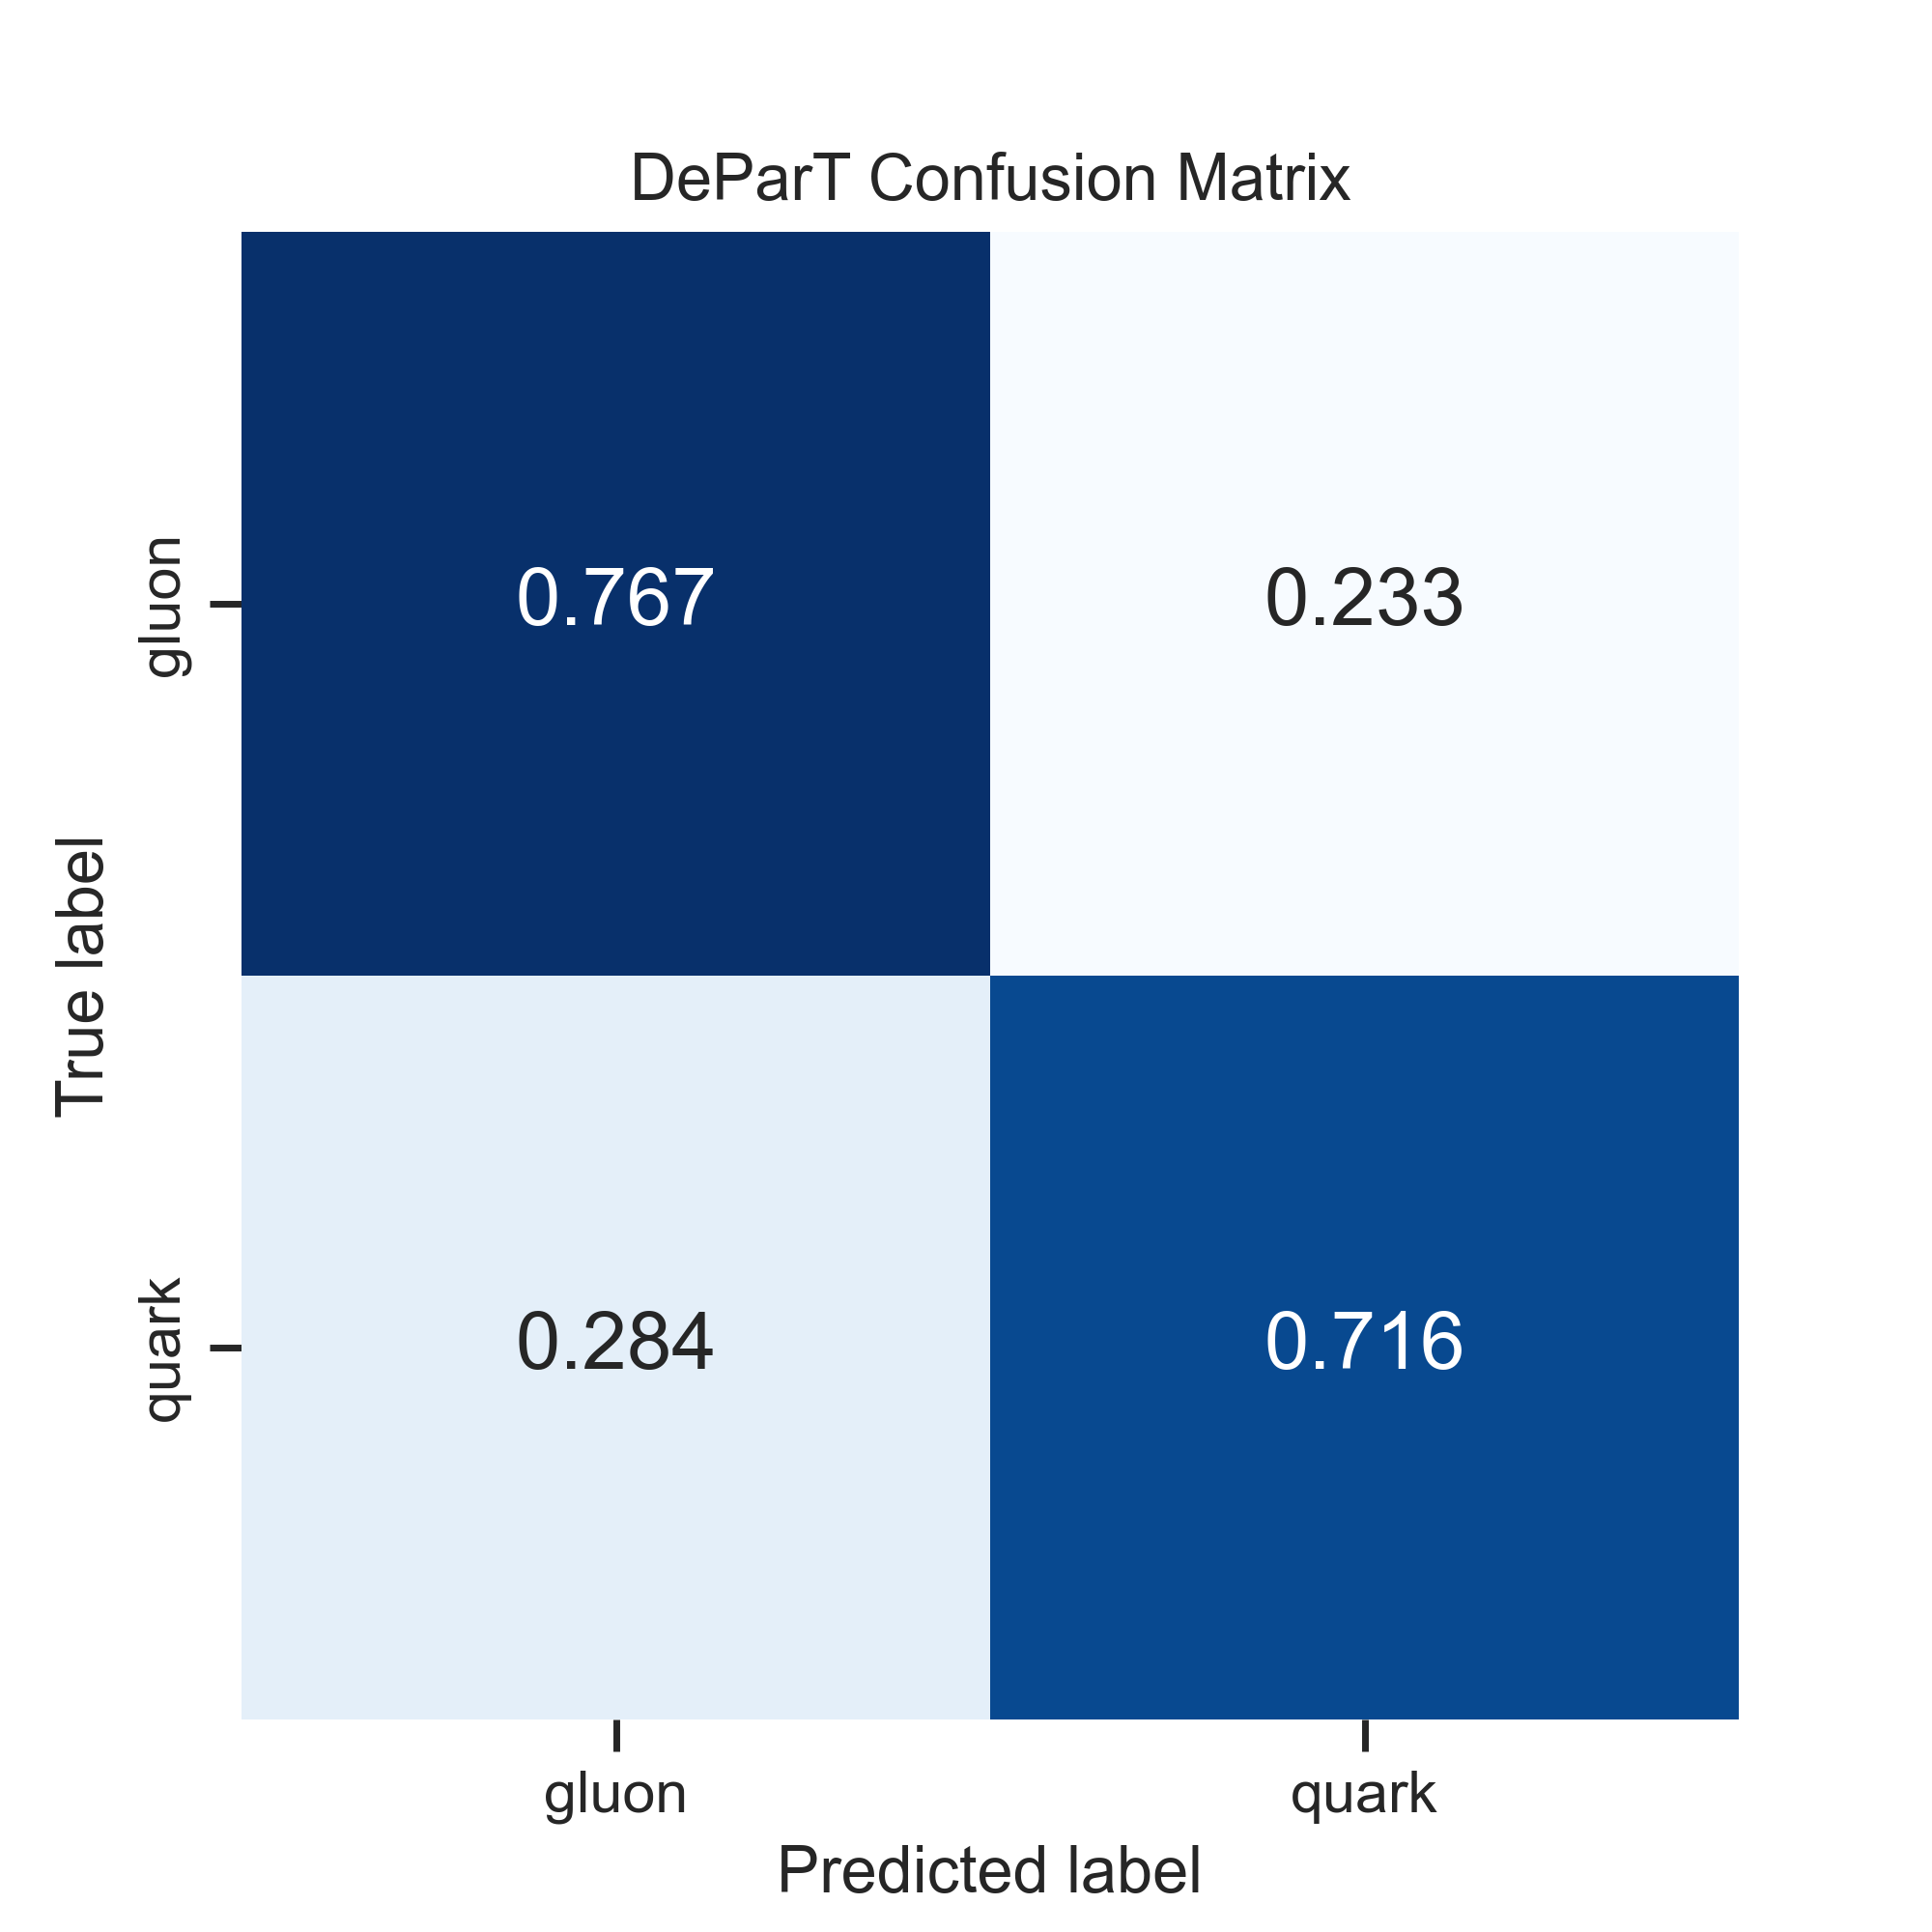
\includegraphics[width=1\textwidth]{src/plots/results/cm/depart.png}
		\caption{DeParT}
		\label{fig:app_cm_depart}
	\end{subfigure}
	\begin{subfigure}[t]{0.38\textwidth}
		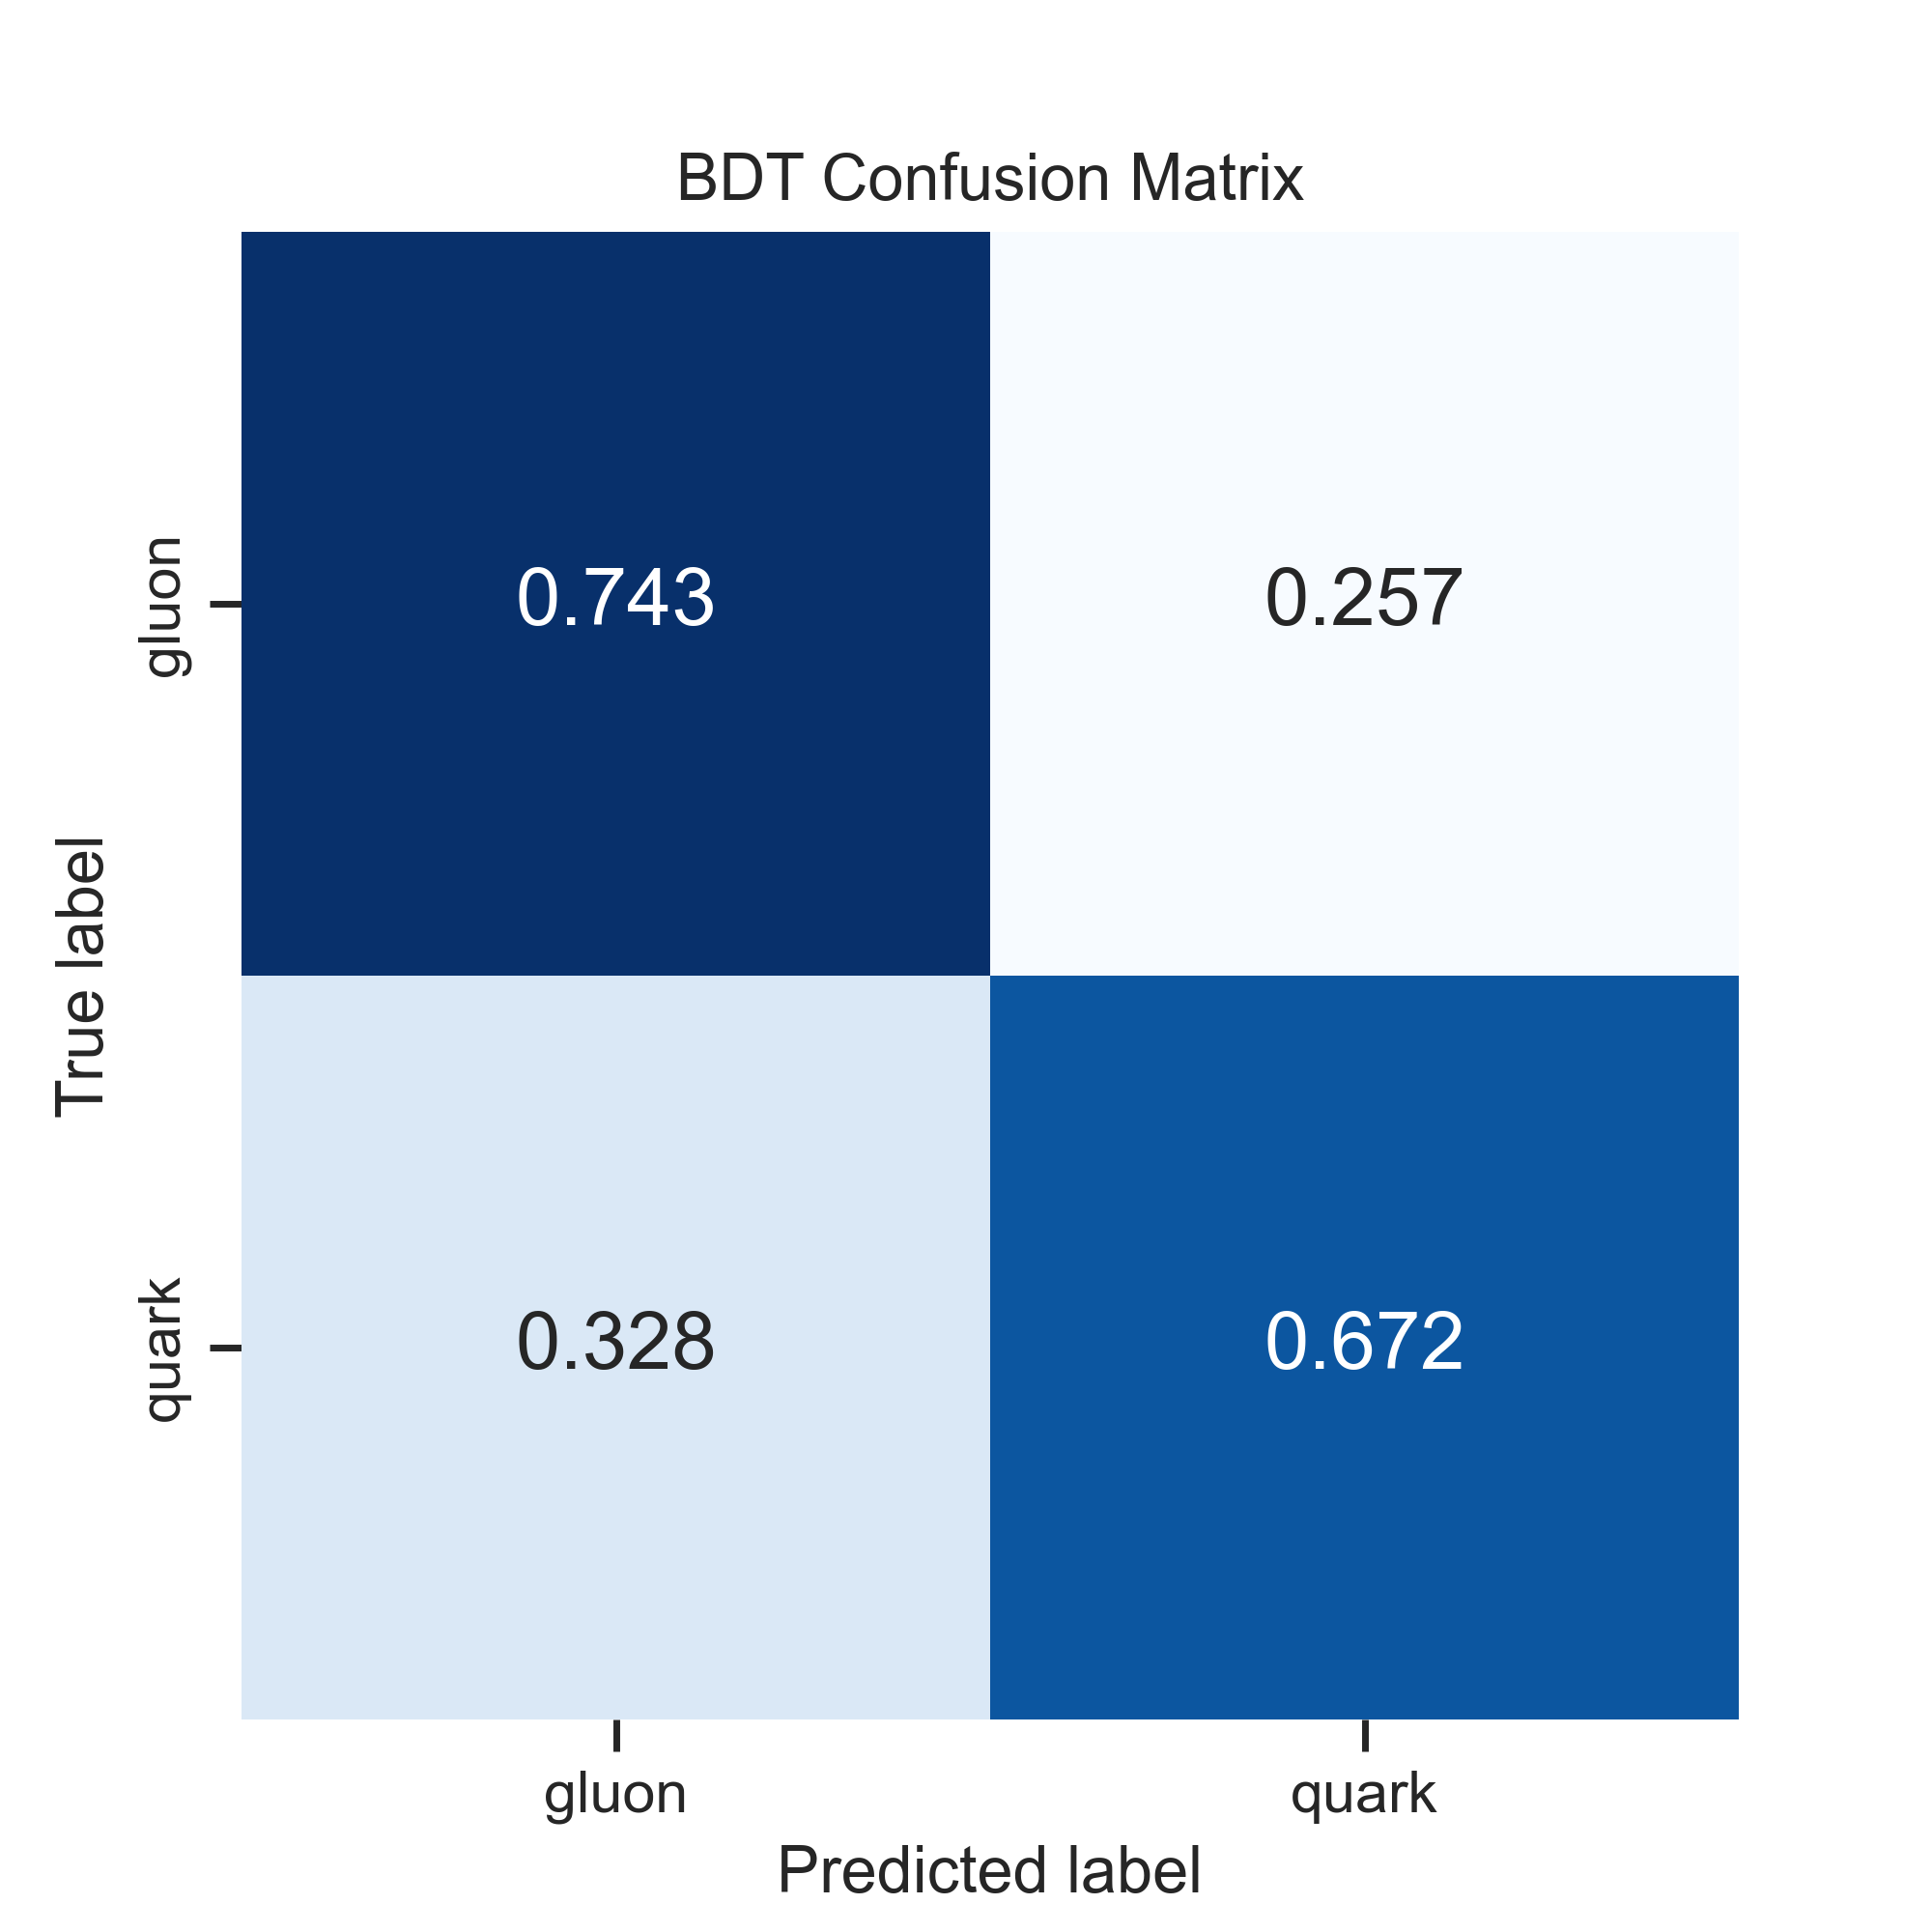
\includegraphics[width=1\textwidth]{src/plots/results/cm/bdt.png}
		\caption{BDT}
		\label{fig:app_cm_bdt}
	\end{subfigure}
	\begin{subfigure}[t]{0.38\textwidth}
		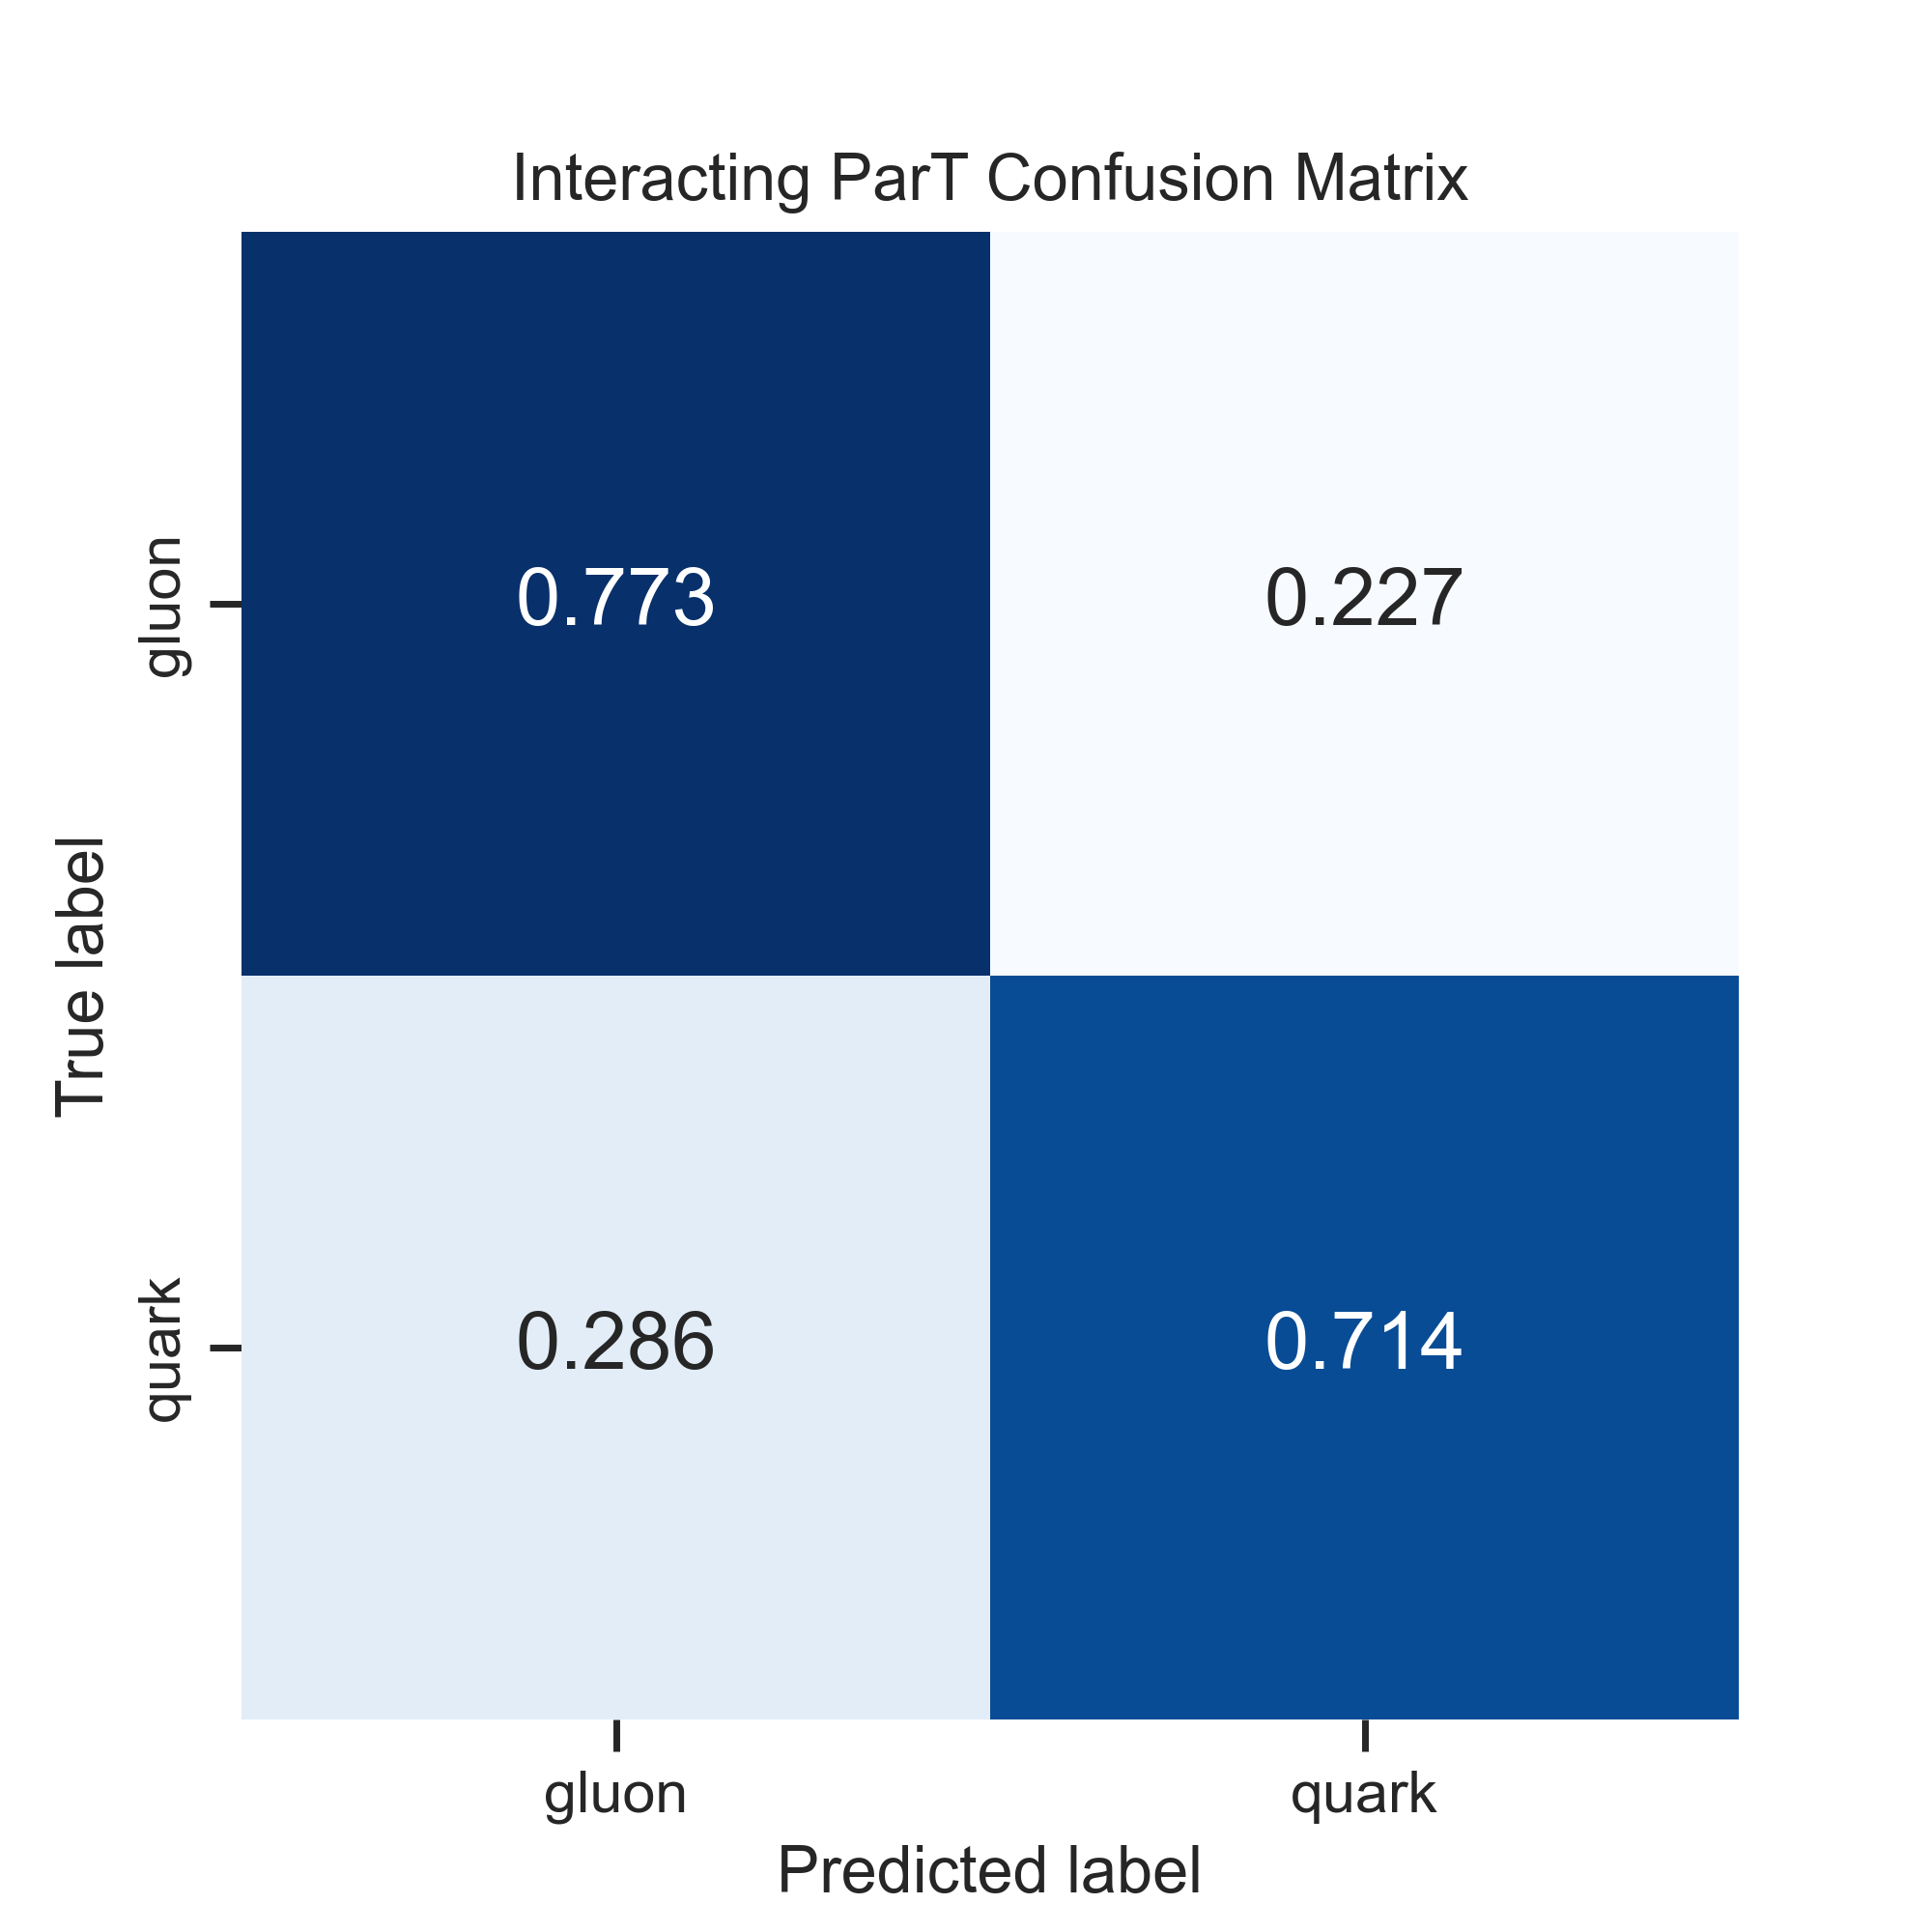
\includegraphics[width=1\textwidth]{src/plots/results/cm/interacting_part.png}
		\caption{Interacting ParT}
		\label{fig:app_cm_interacting_part}
	\end{subfigure}
	\begin{subfigure}[t]{0.38\textwidth}
		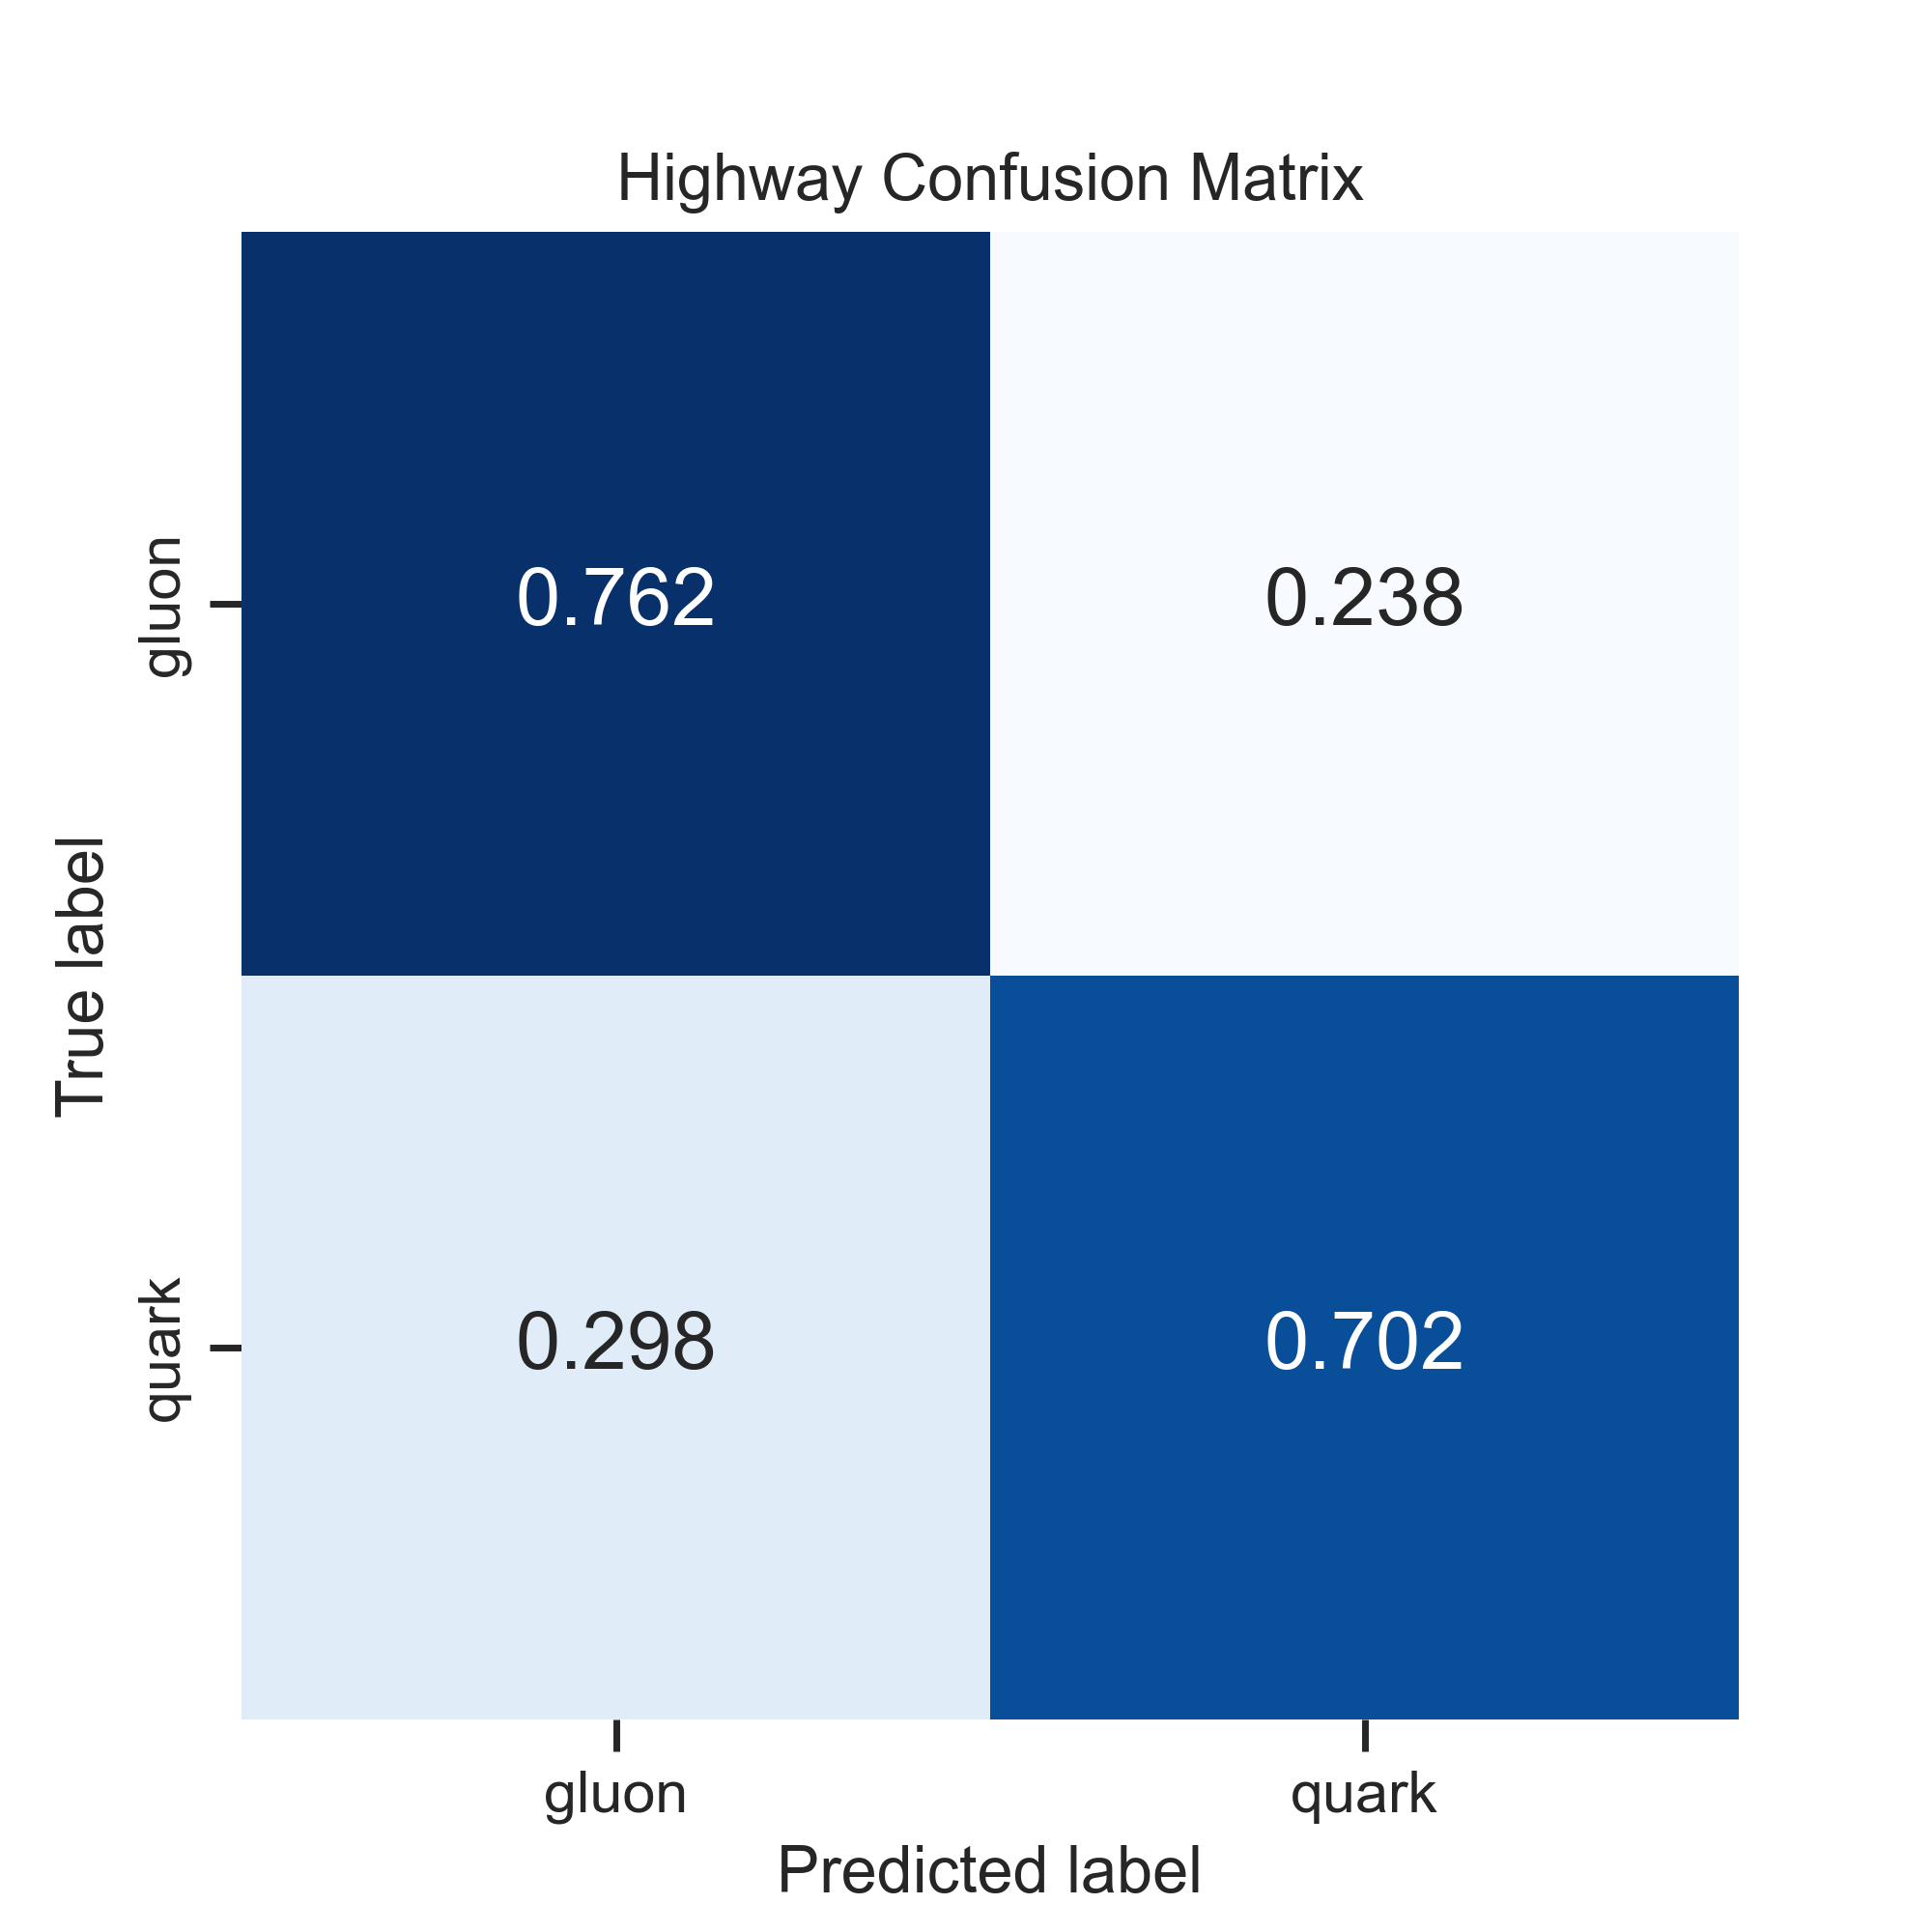
\includegraphics[width=1\textwidth]{src/plots/results/cm/highway.png}
		\caption{Highway}
		\label{fig:app_cm_highway}
	\end{subfigure}
\caption{Confusion Matricies}
\label{fig:app_cm_-1-3}
\end{figure}

\begin{figure}[!htb]
	\centering
	\begin{subfigure}[t]{0.38\textwidth}
		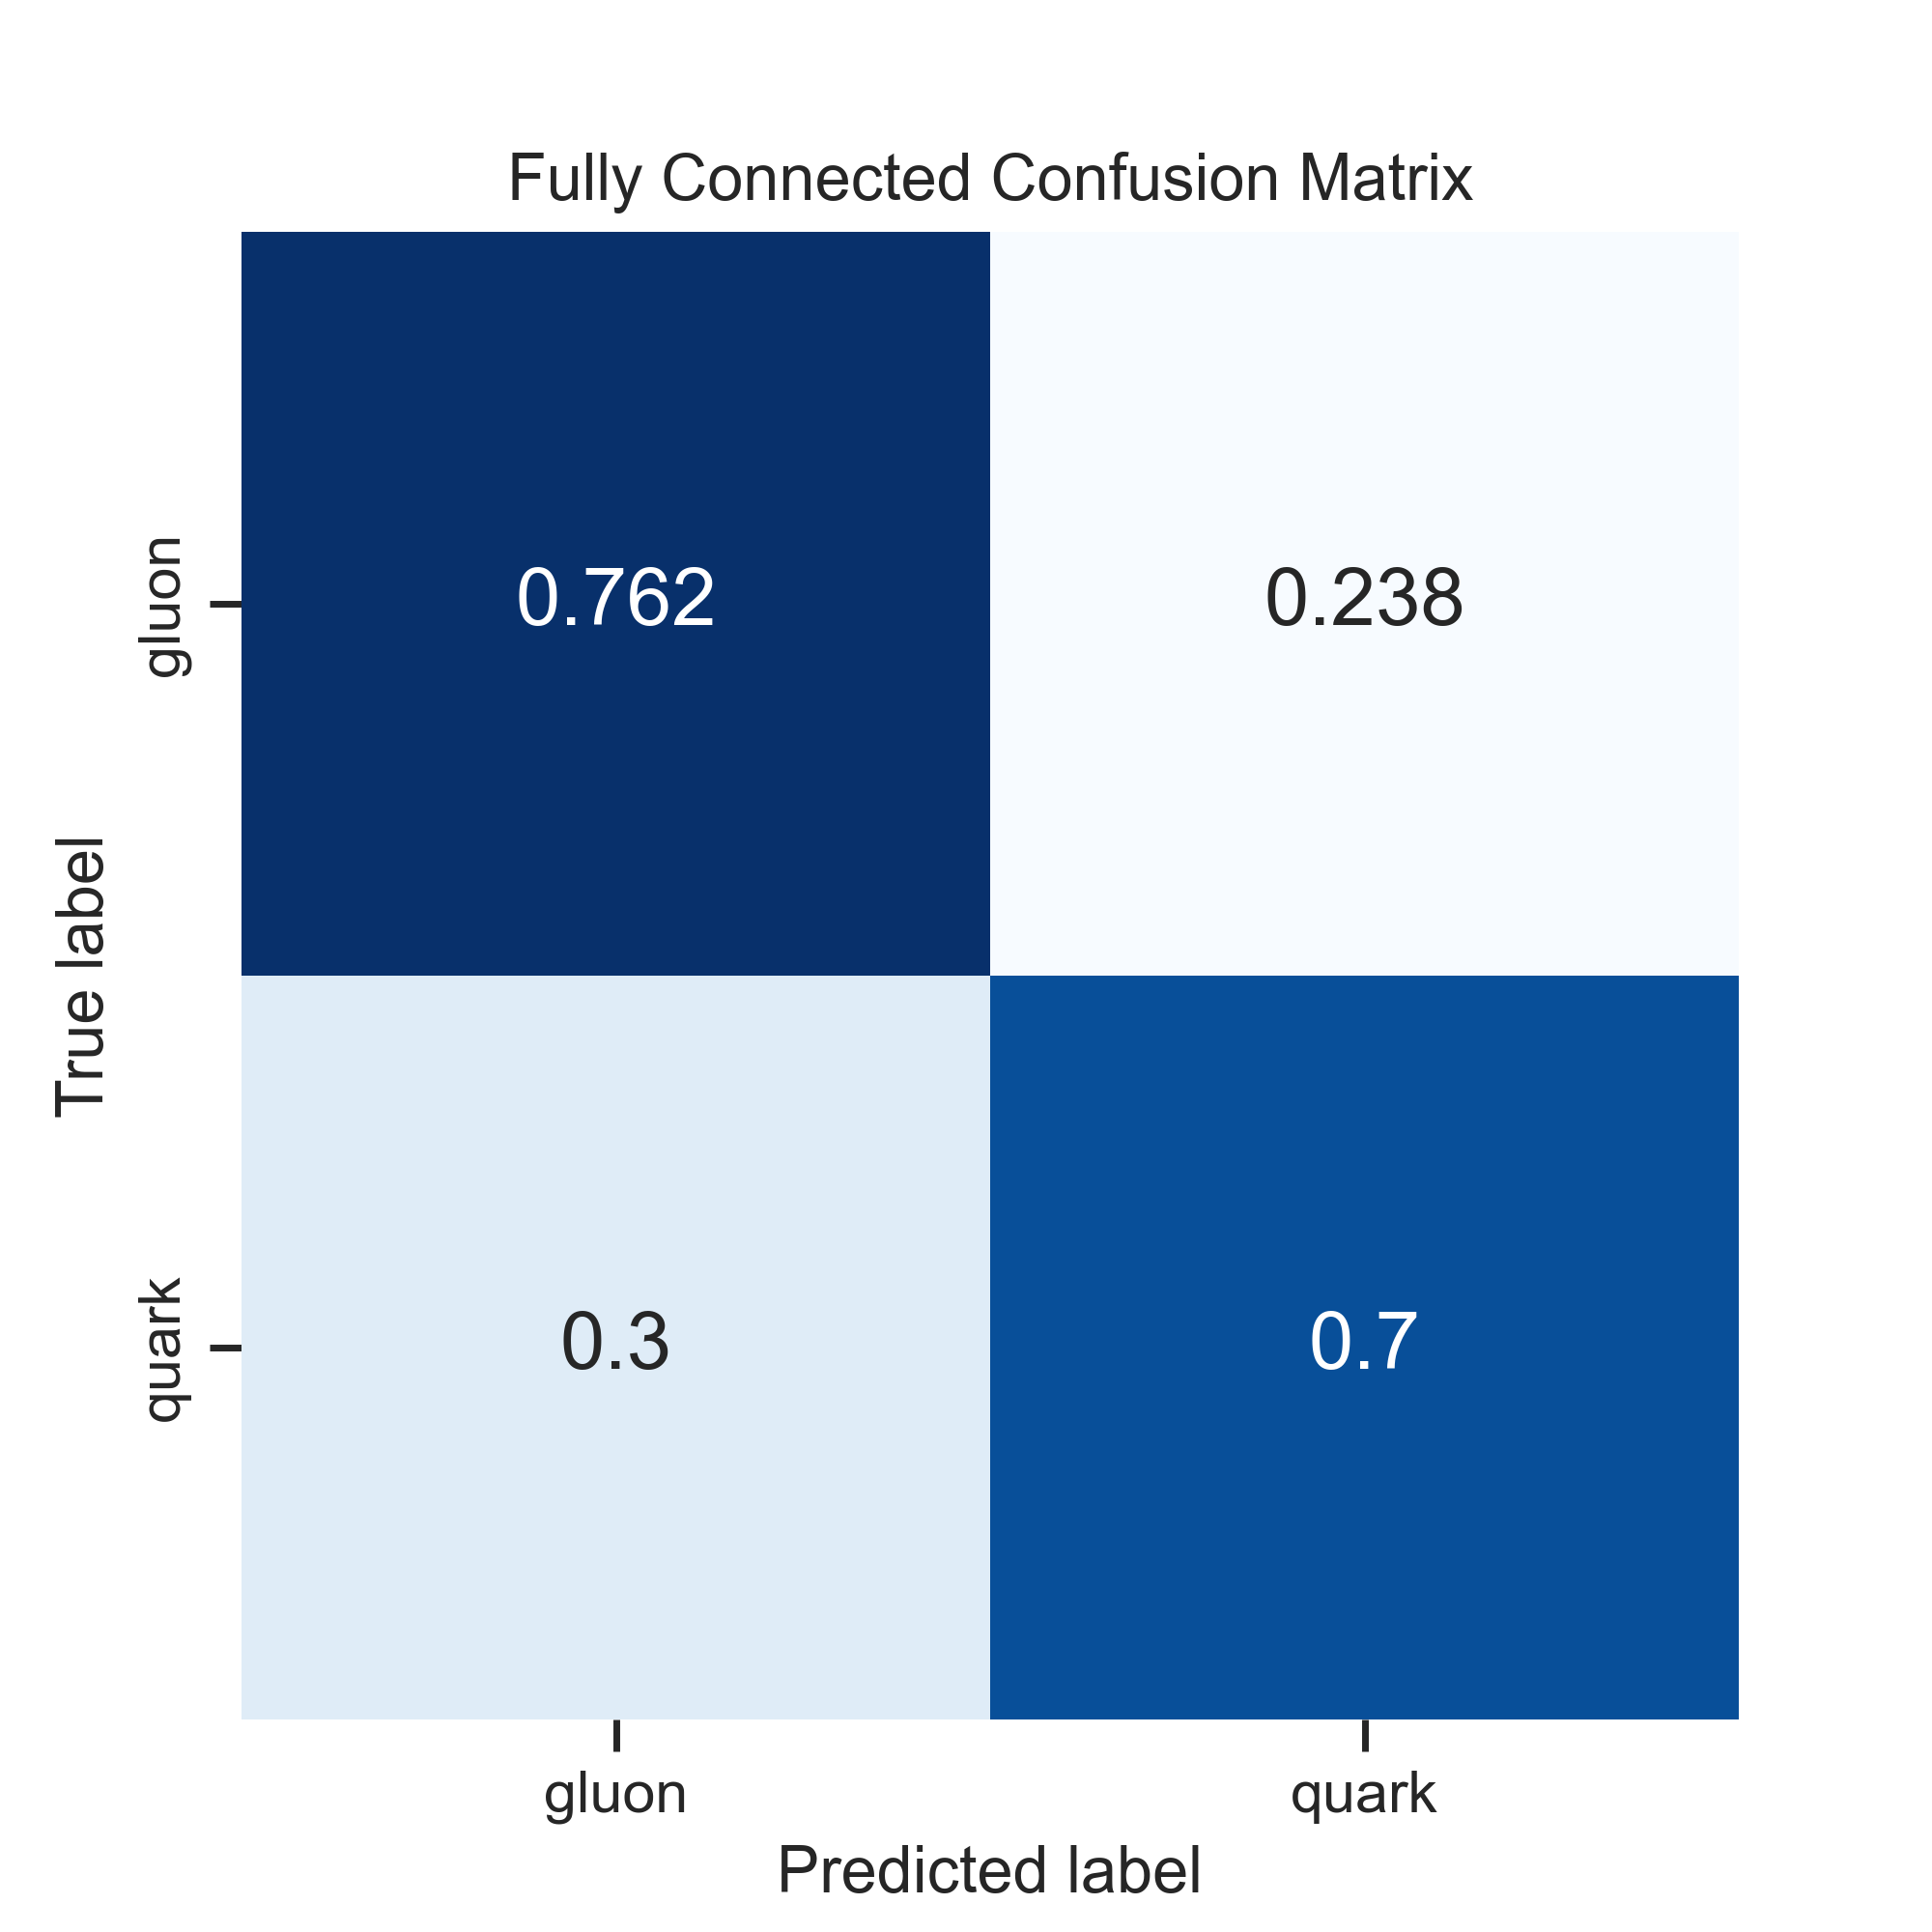
\includegraphics[width=1\textwidth]{src/plots/results/cm/fc.png}
		\caption{Fully Connected}
		\label{fig:app_cm_fc}
	\end{subfigure}
	\begin{subfigure}[t]{0.38\textwidth}
		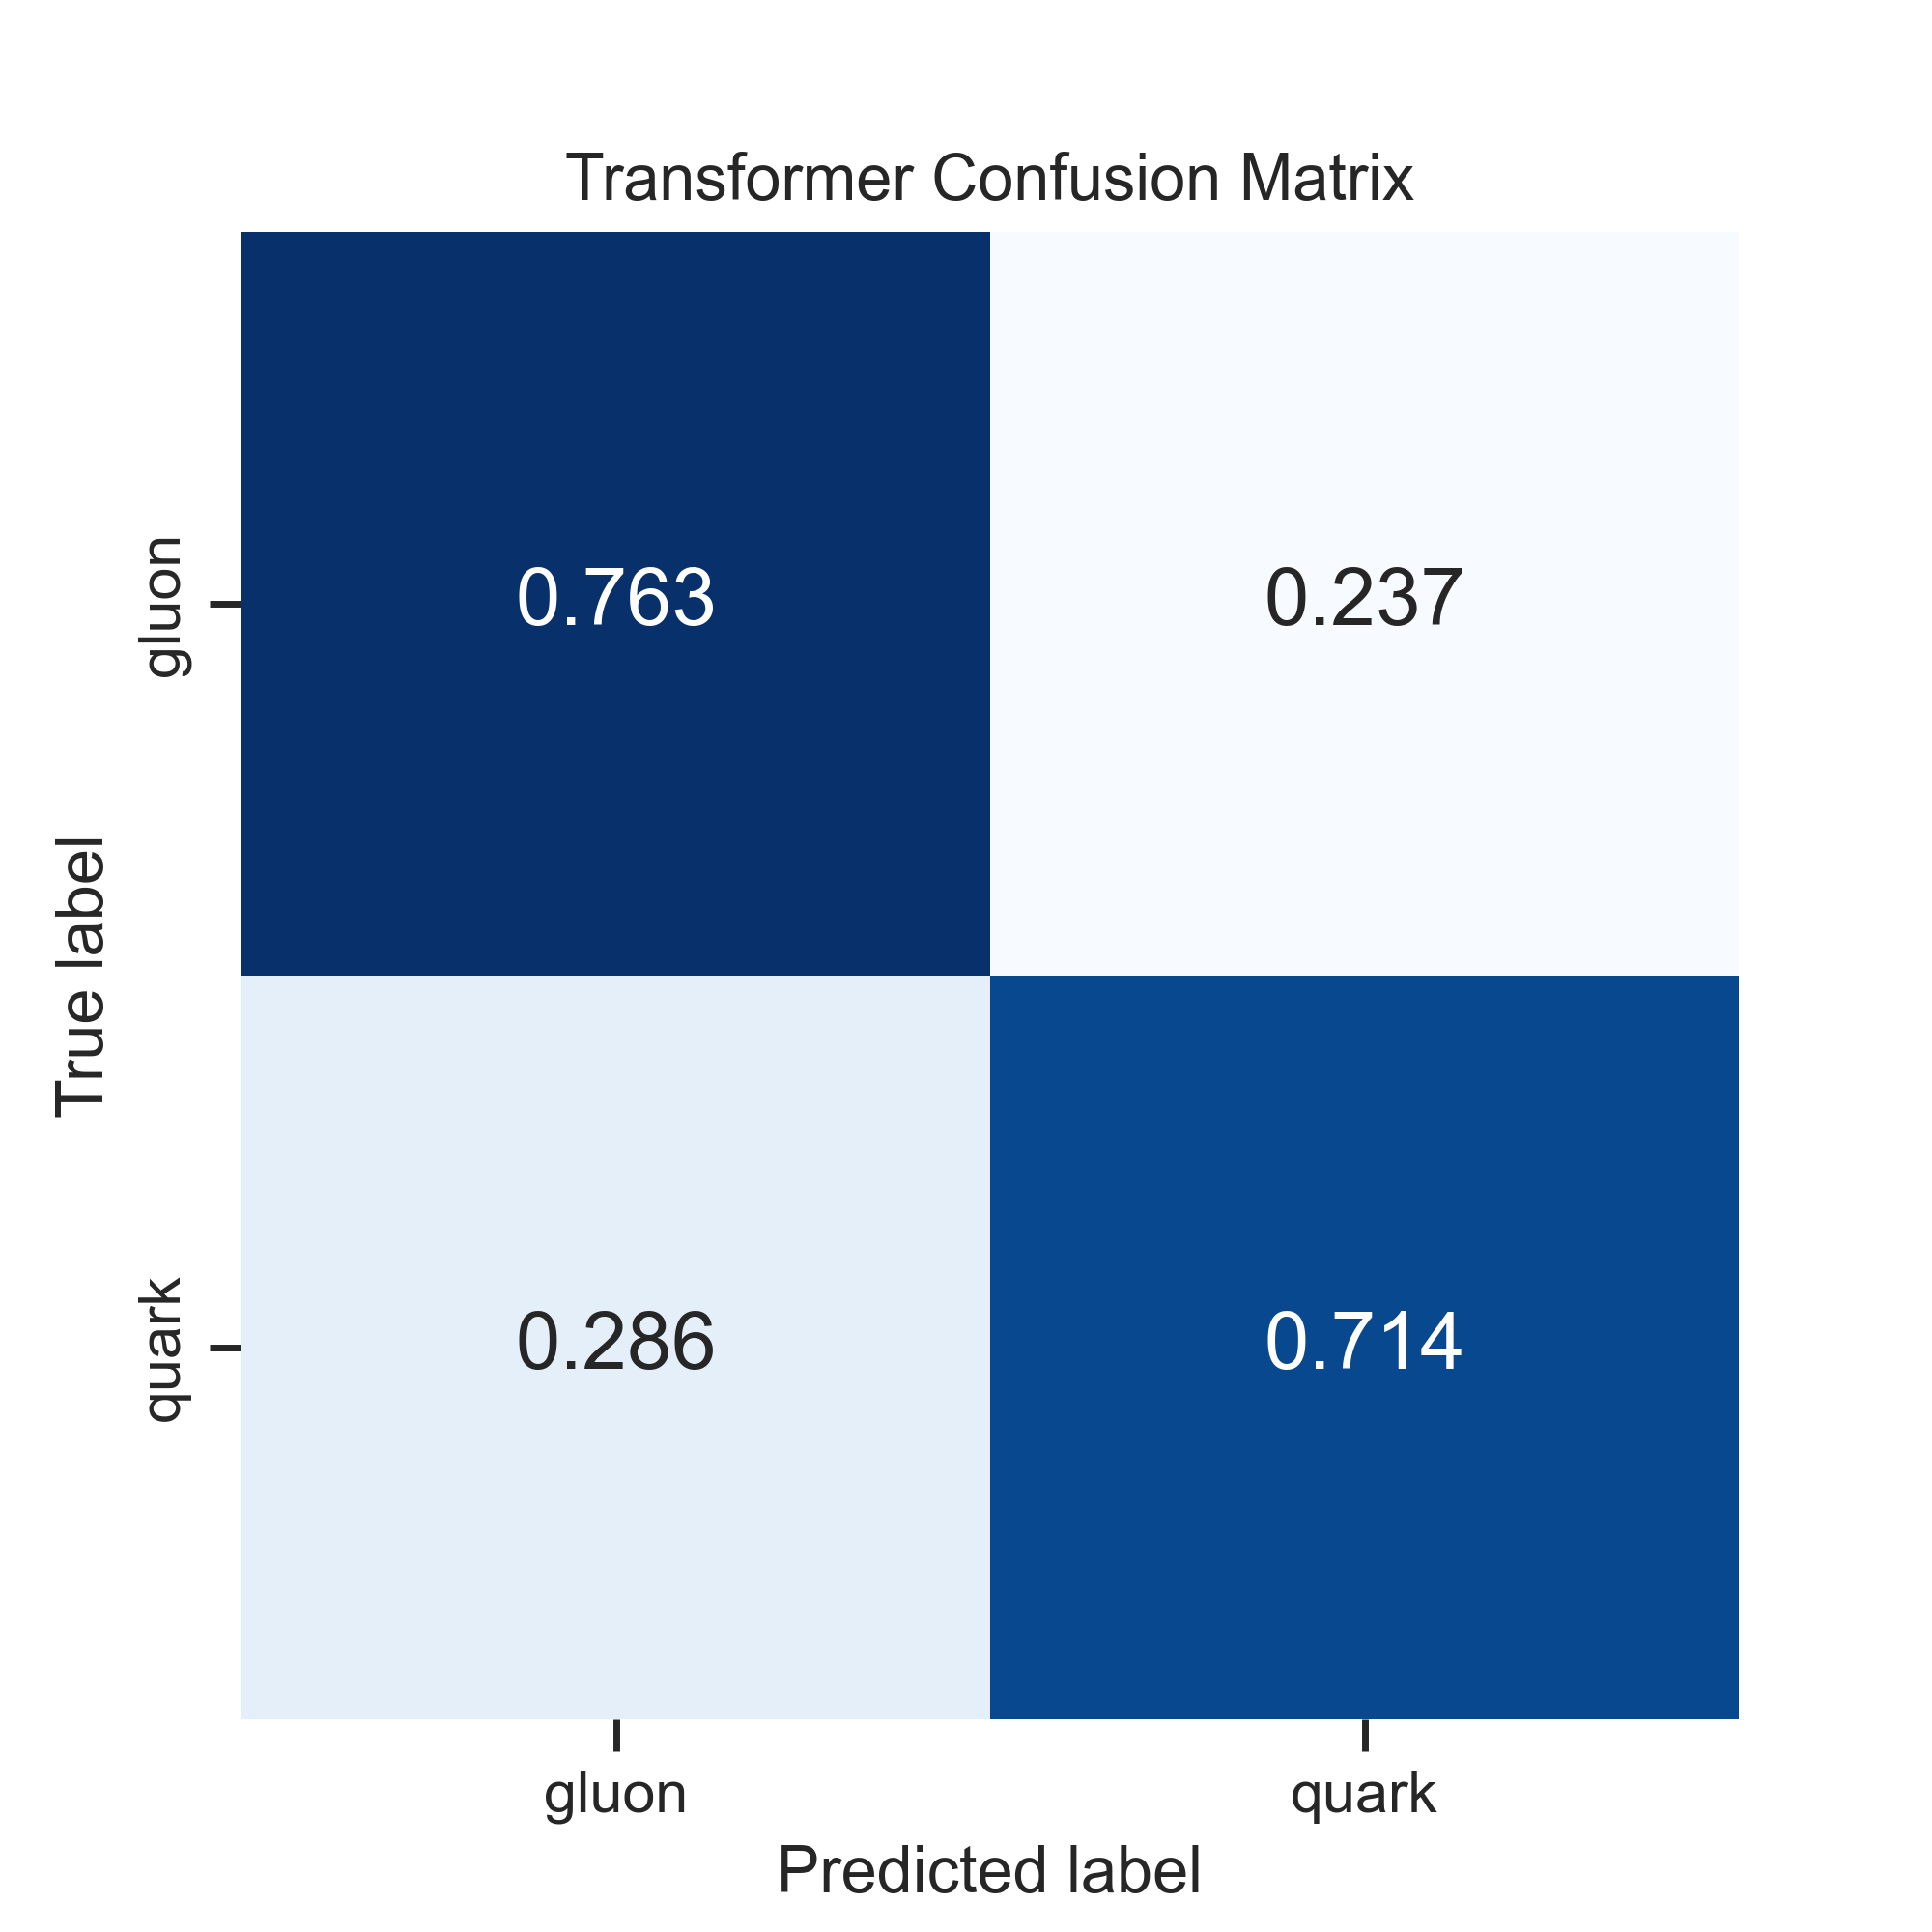
\includegraphics[width=1\textwidth]{src/plots/results/cm/transformer.png}
		\caption{Transformer}
		\label{fig:app_cm_transformer}
	\end{subfigure}
	\begin{subfigure}[t]{0.38\textwidth}
		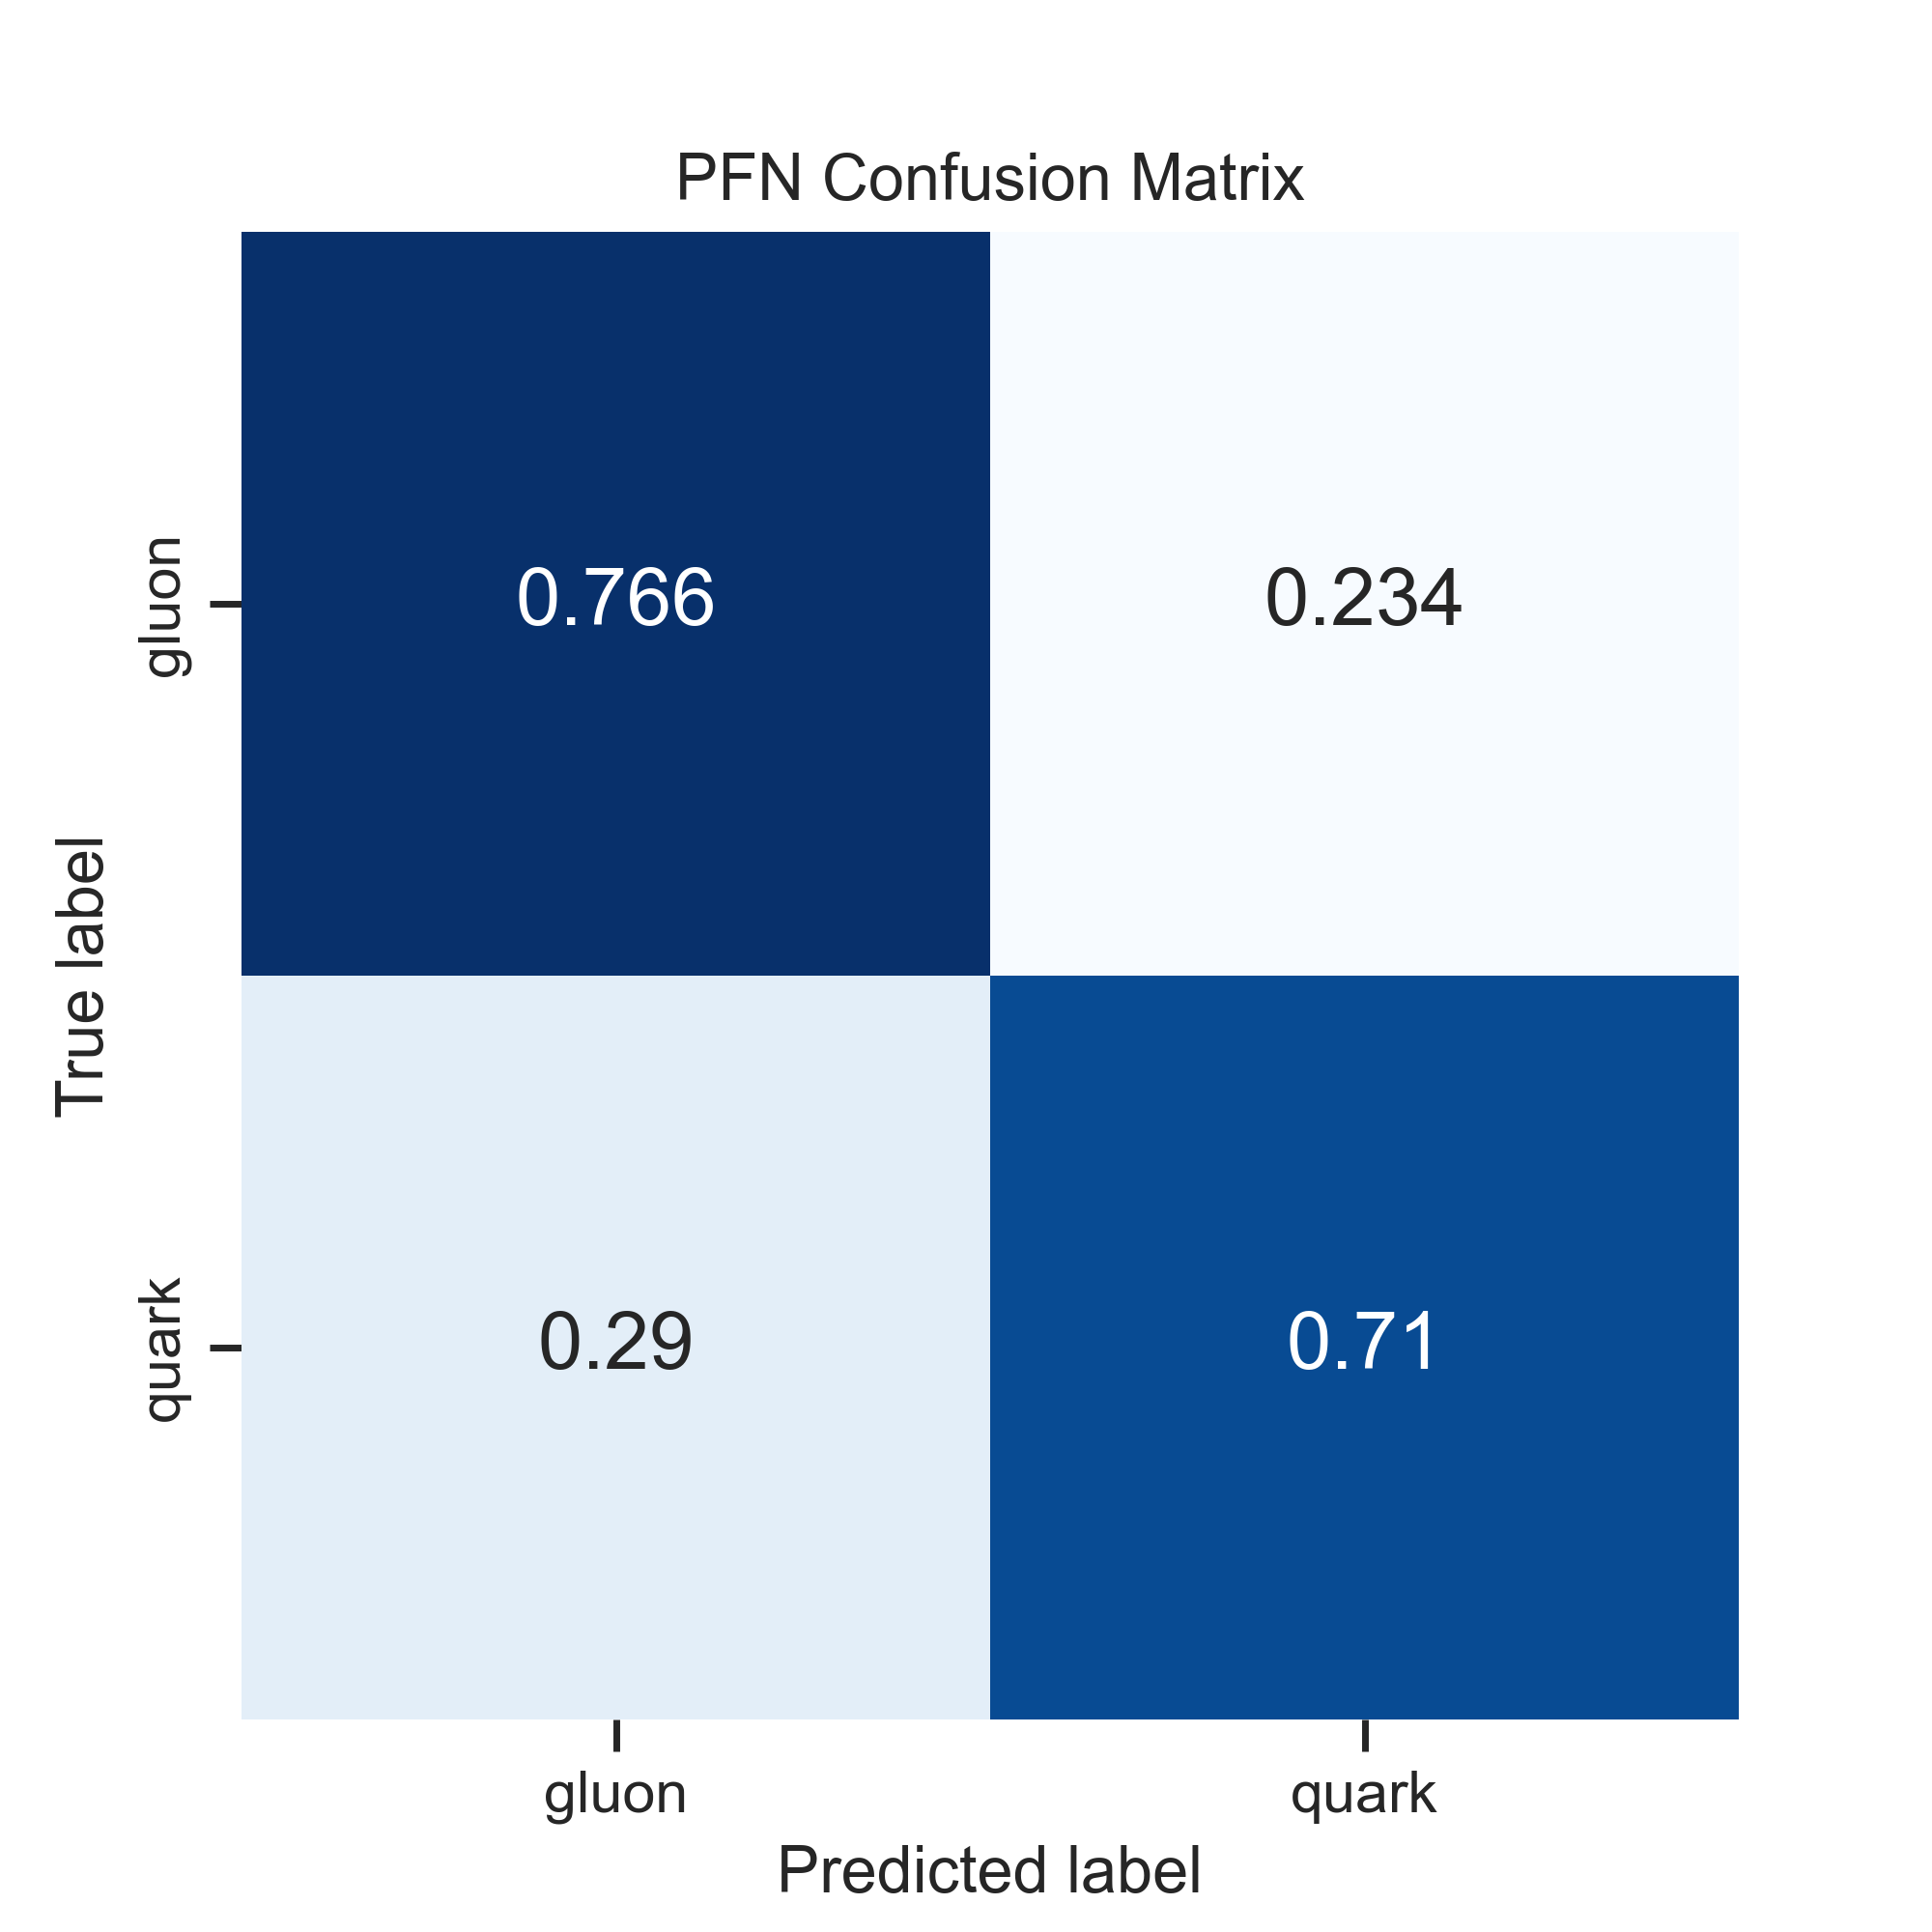
\includegraphics[width=1\textwidth]{src/plots/results/cm/pfn.png}
		\caption{PFN}
		\label{fig:app_cm_pfn}
	\end{subfigure}
	\begin{subfigure}[t]{0.38\textwidth}
		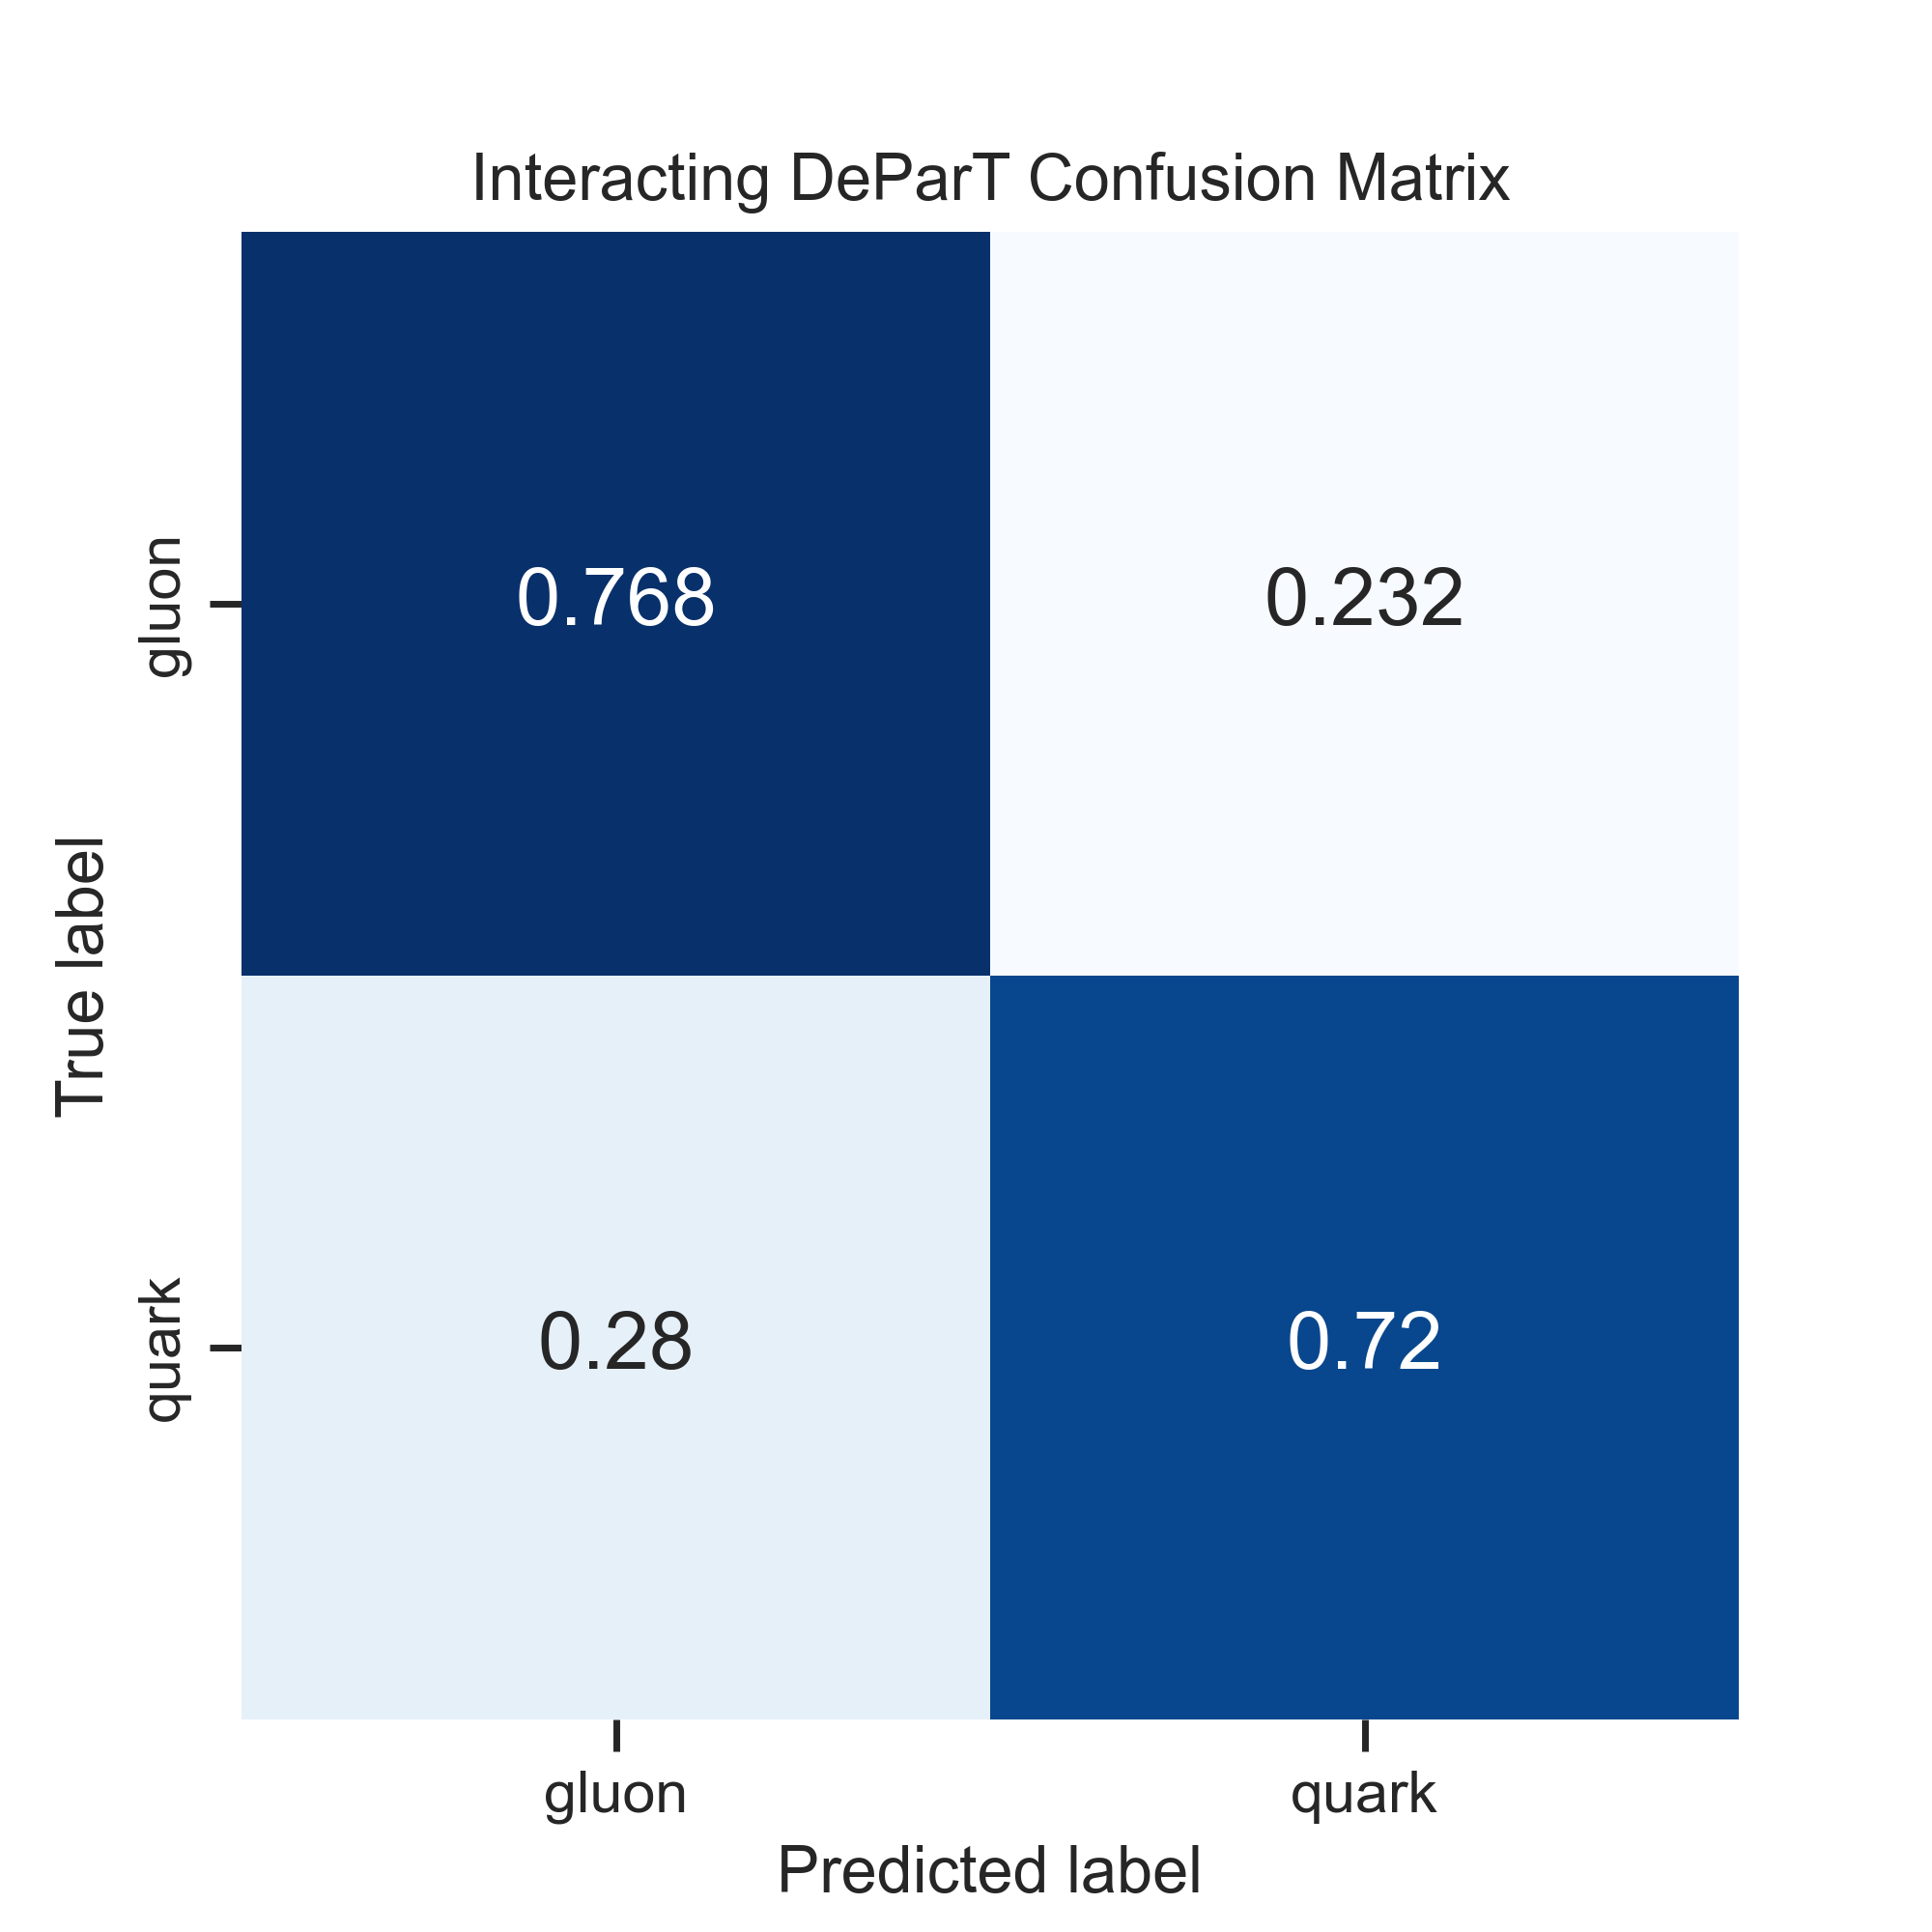
\includegraphics[width=1\textwidth]{src/plots/results/cm/interacting_depart.png}
		\caption{Interacting DeParT}
		\label{fig:app_cm_interacting_depart}
	\end{subfigure}
	\begin{subfigure}[t]{0.38\textwidth}
		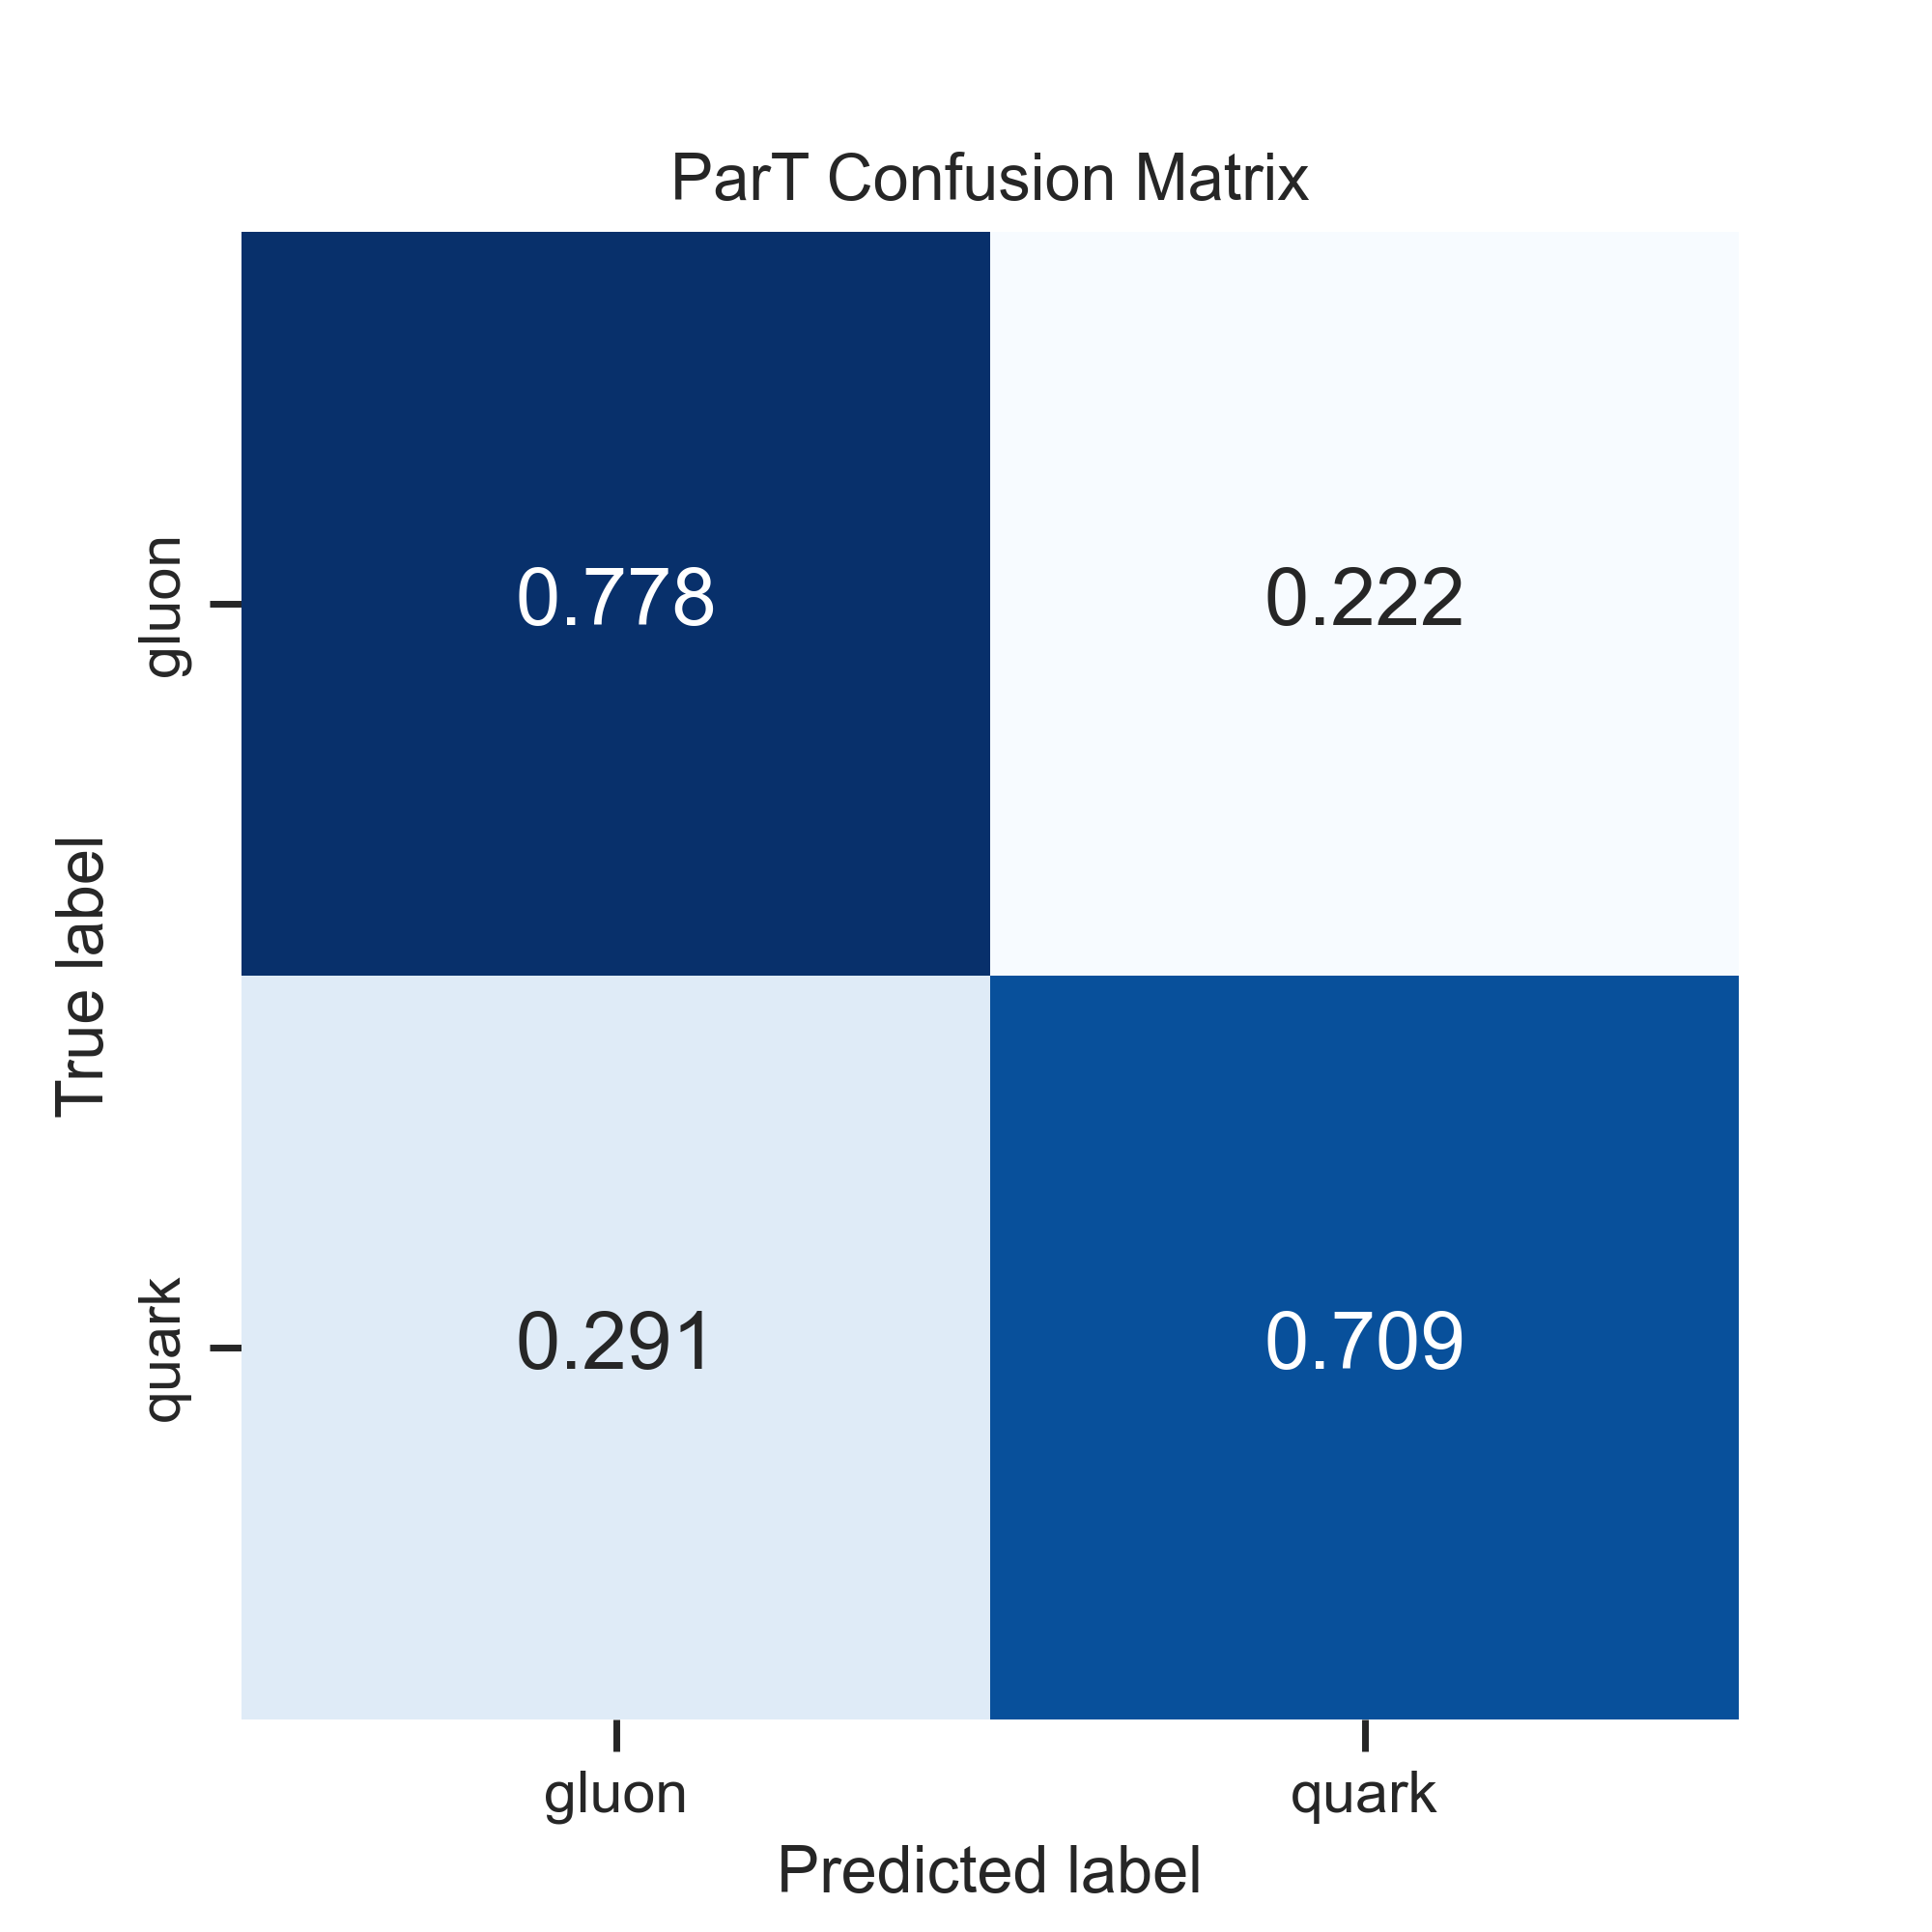
\includegraphics[width=1\textwidth]{src/plots/results/cm/part.png}
		\caption{ParT}
		\label{fig:app_cm_part}
	\end{subfigure}
	\begin{subfigure}[t]{0.38\textwidth}
		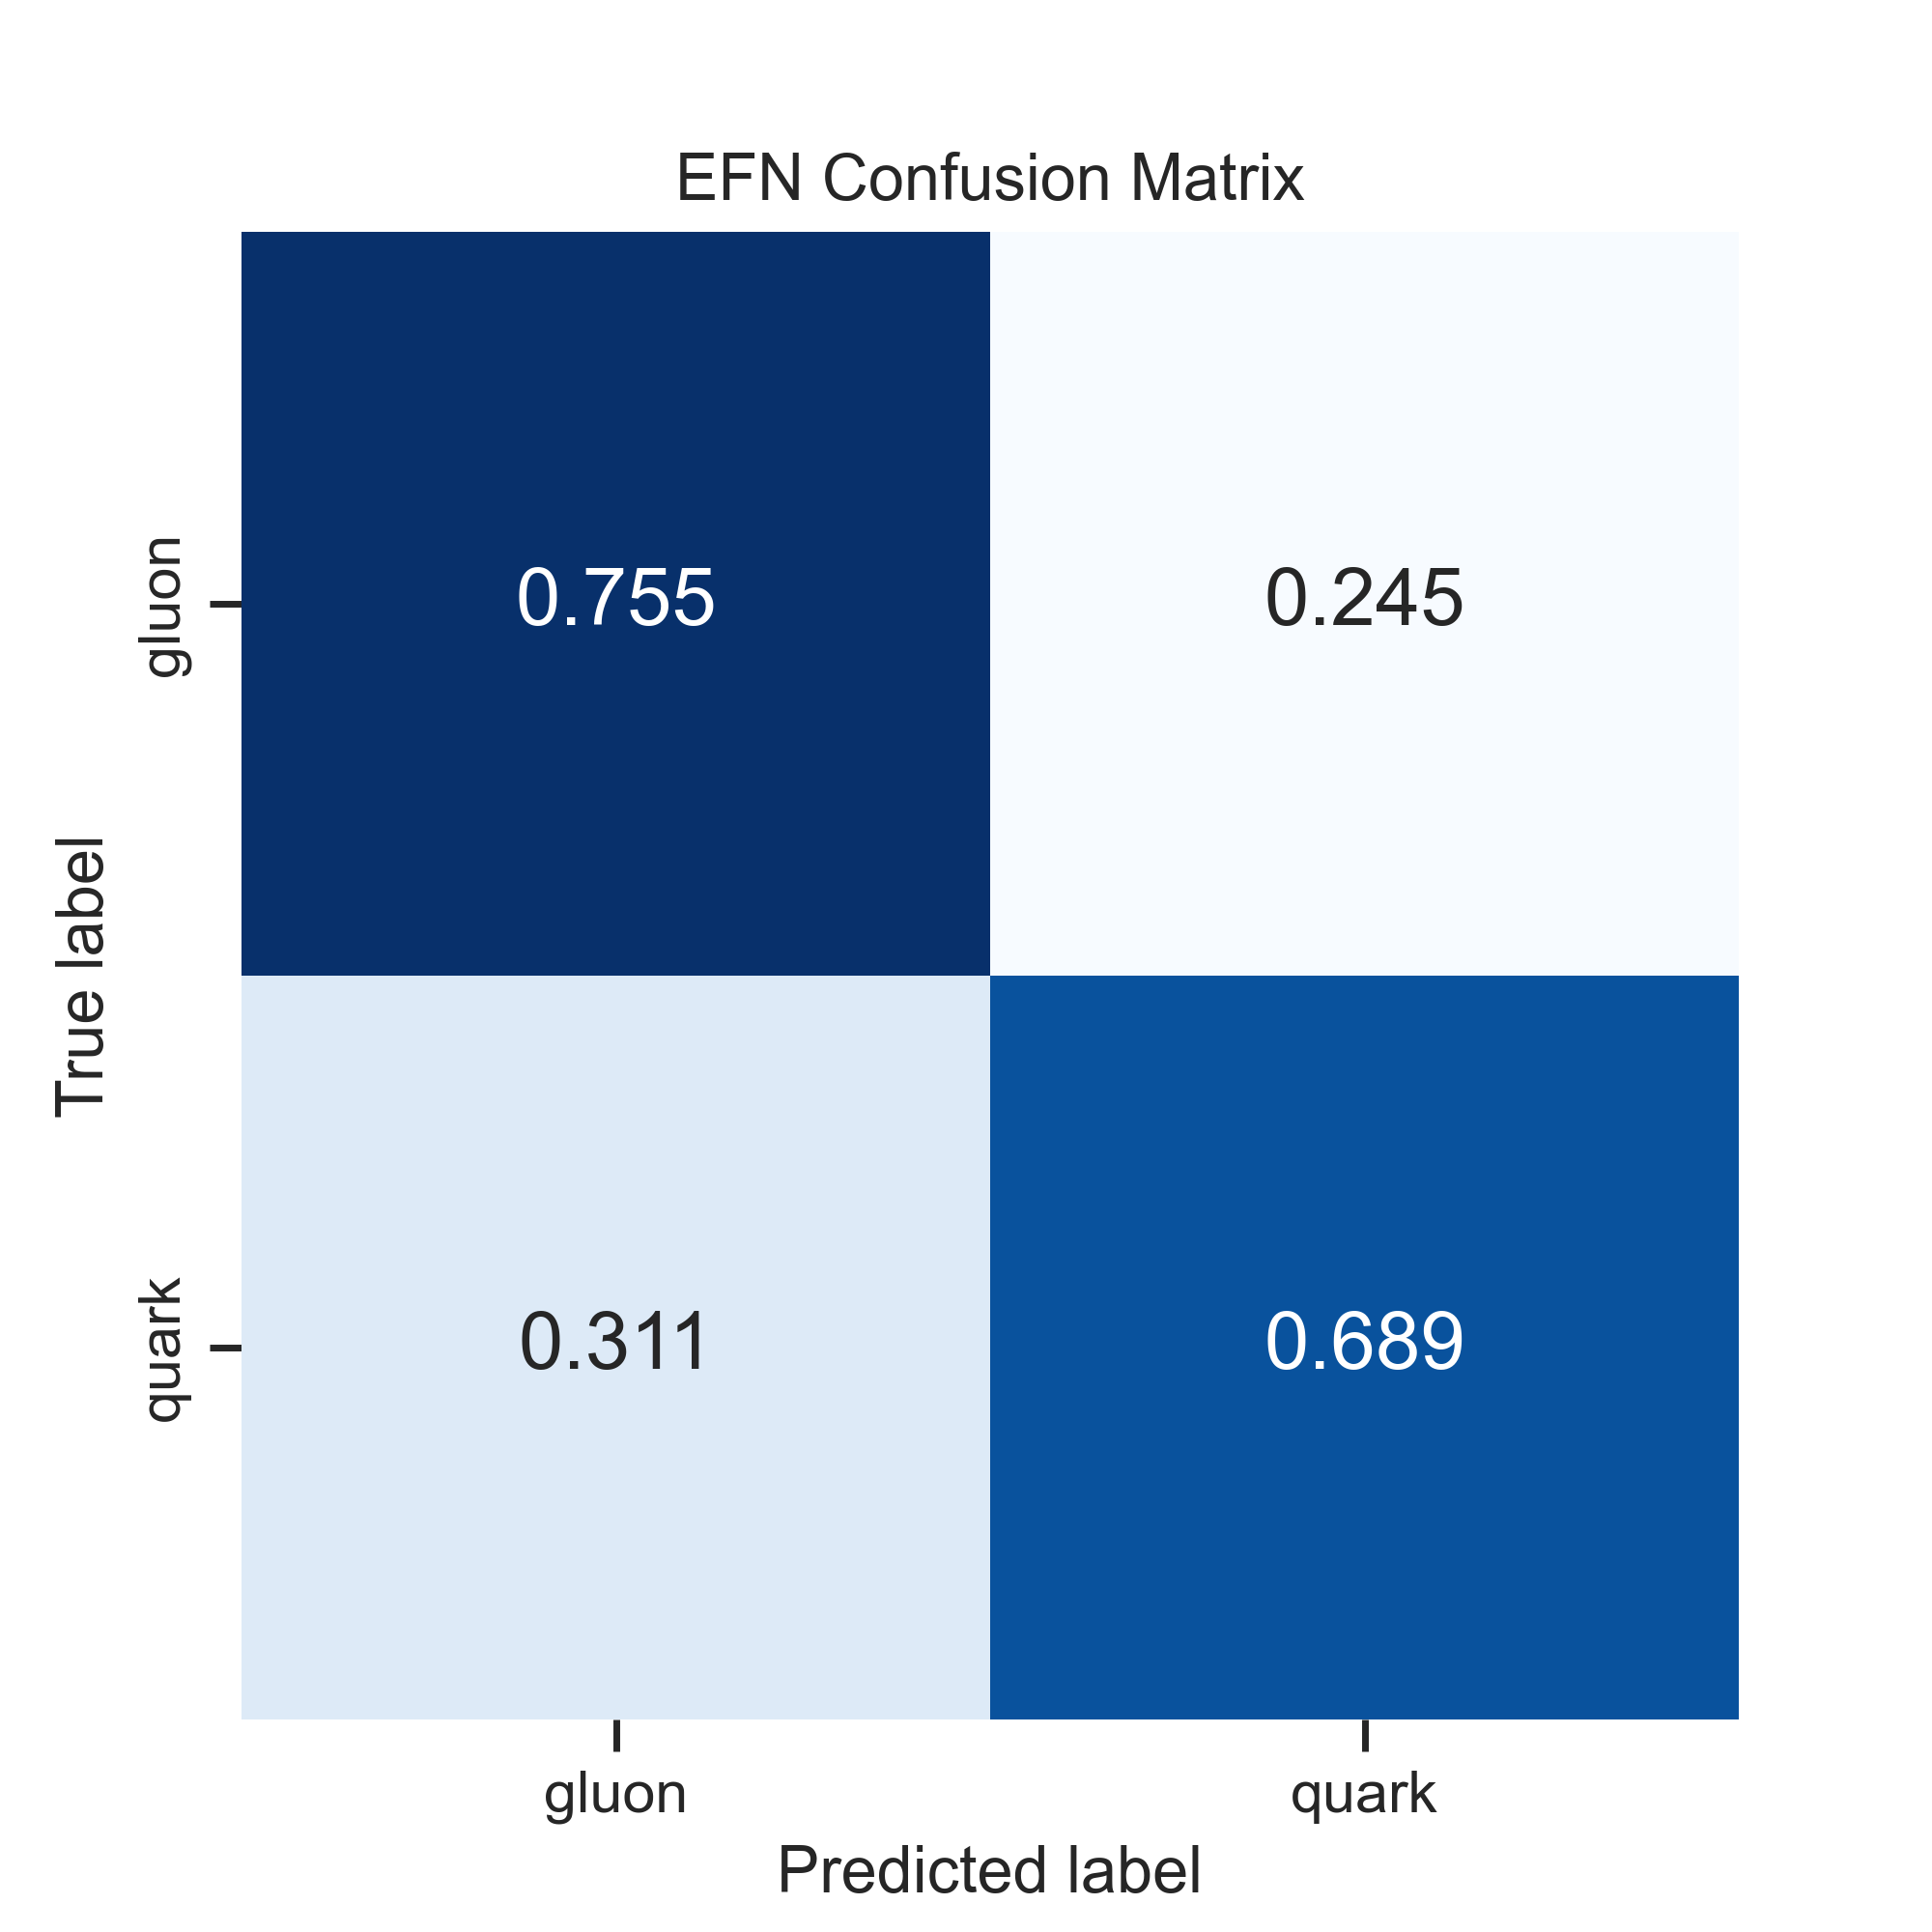
\includegraphics[width=1\textwidth]{src/plots/results/cm/efn.png}
		\caption{EFN}
		\label{fig:app_cm_efn}
	\end{subfigure}
\caption{Confusion Matricies}
\label{fig:app_cm_5-9}
\end{figure}



\FloatBarrier
\newpage

\section{Score Histograms}
\label{sec:app_scorehist}

\begin{figure}[!htb]
	\centering
	\begin{subfigure}[t]{0.49\textwidth}
		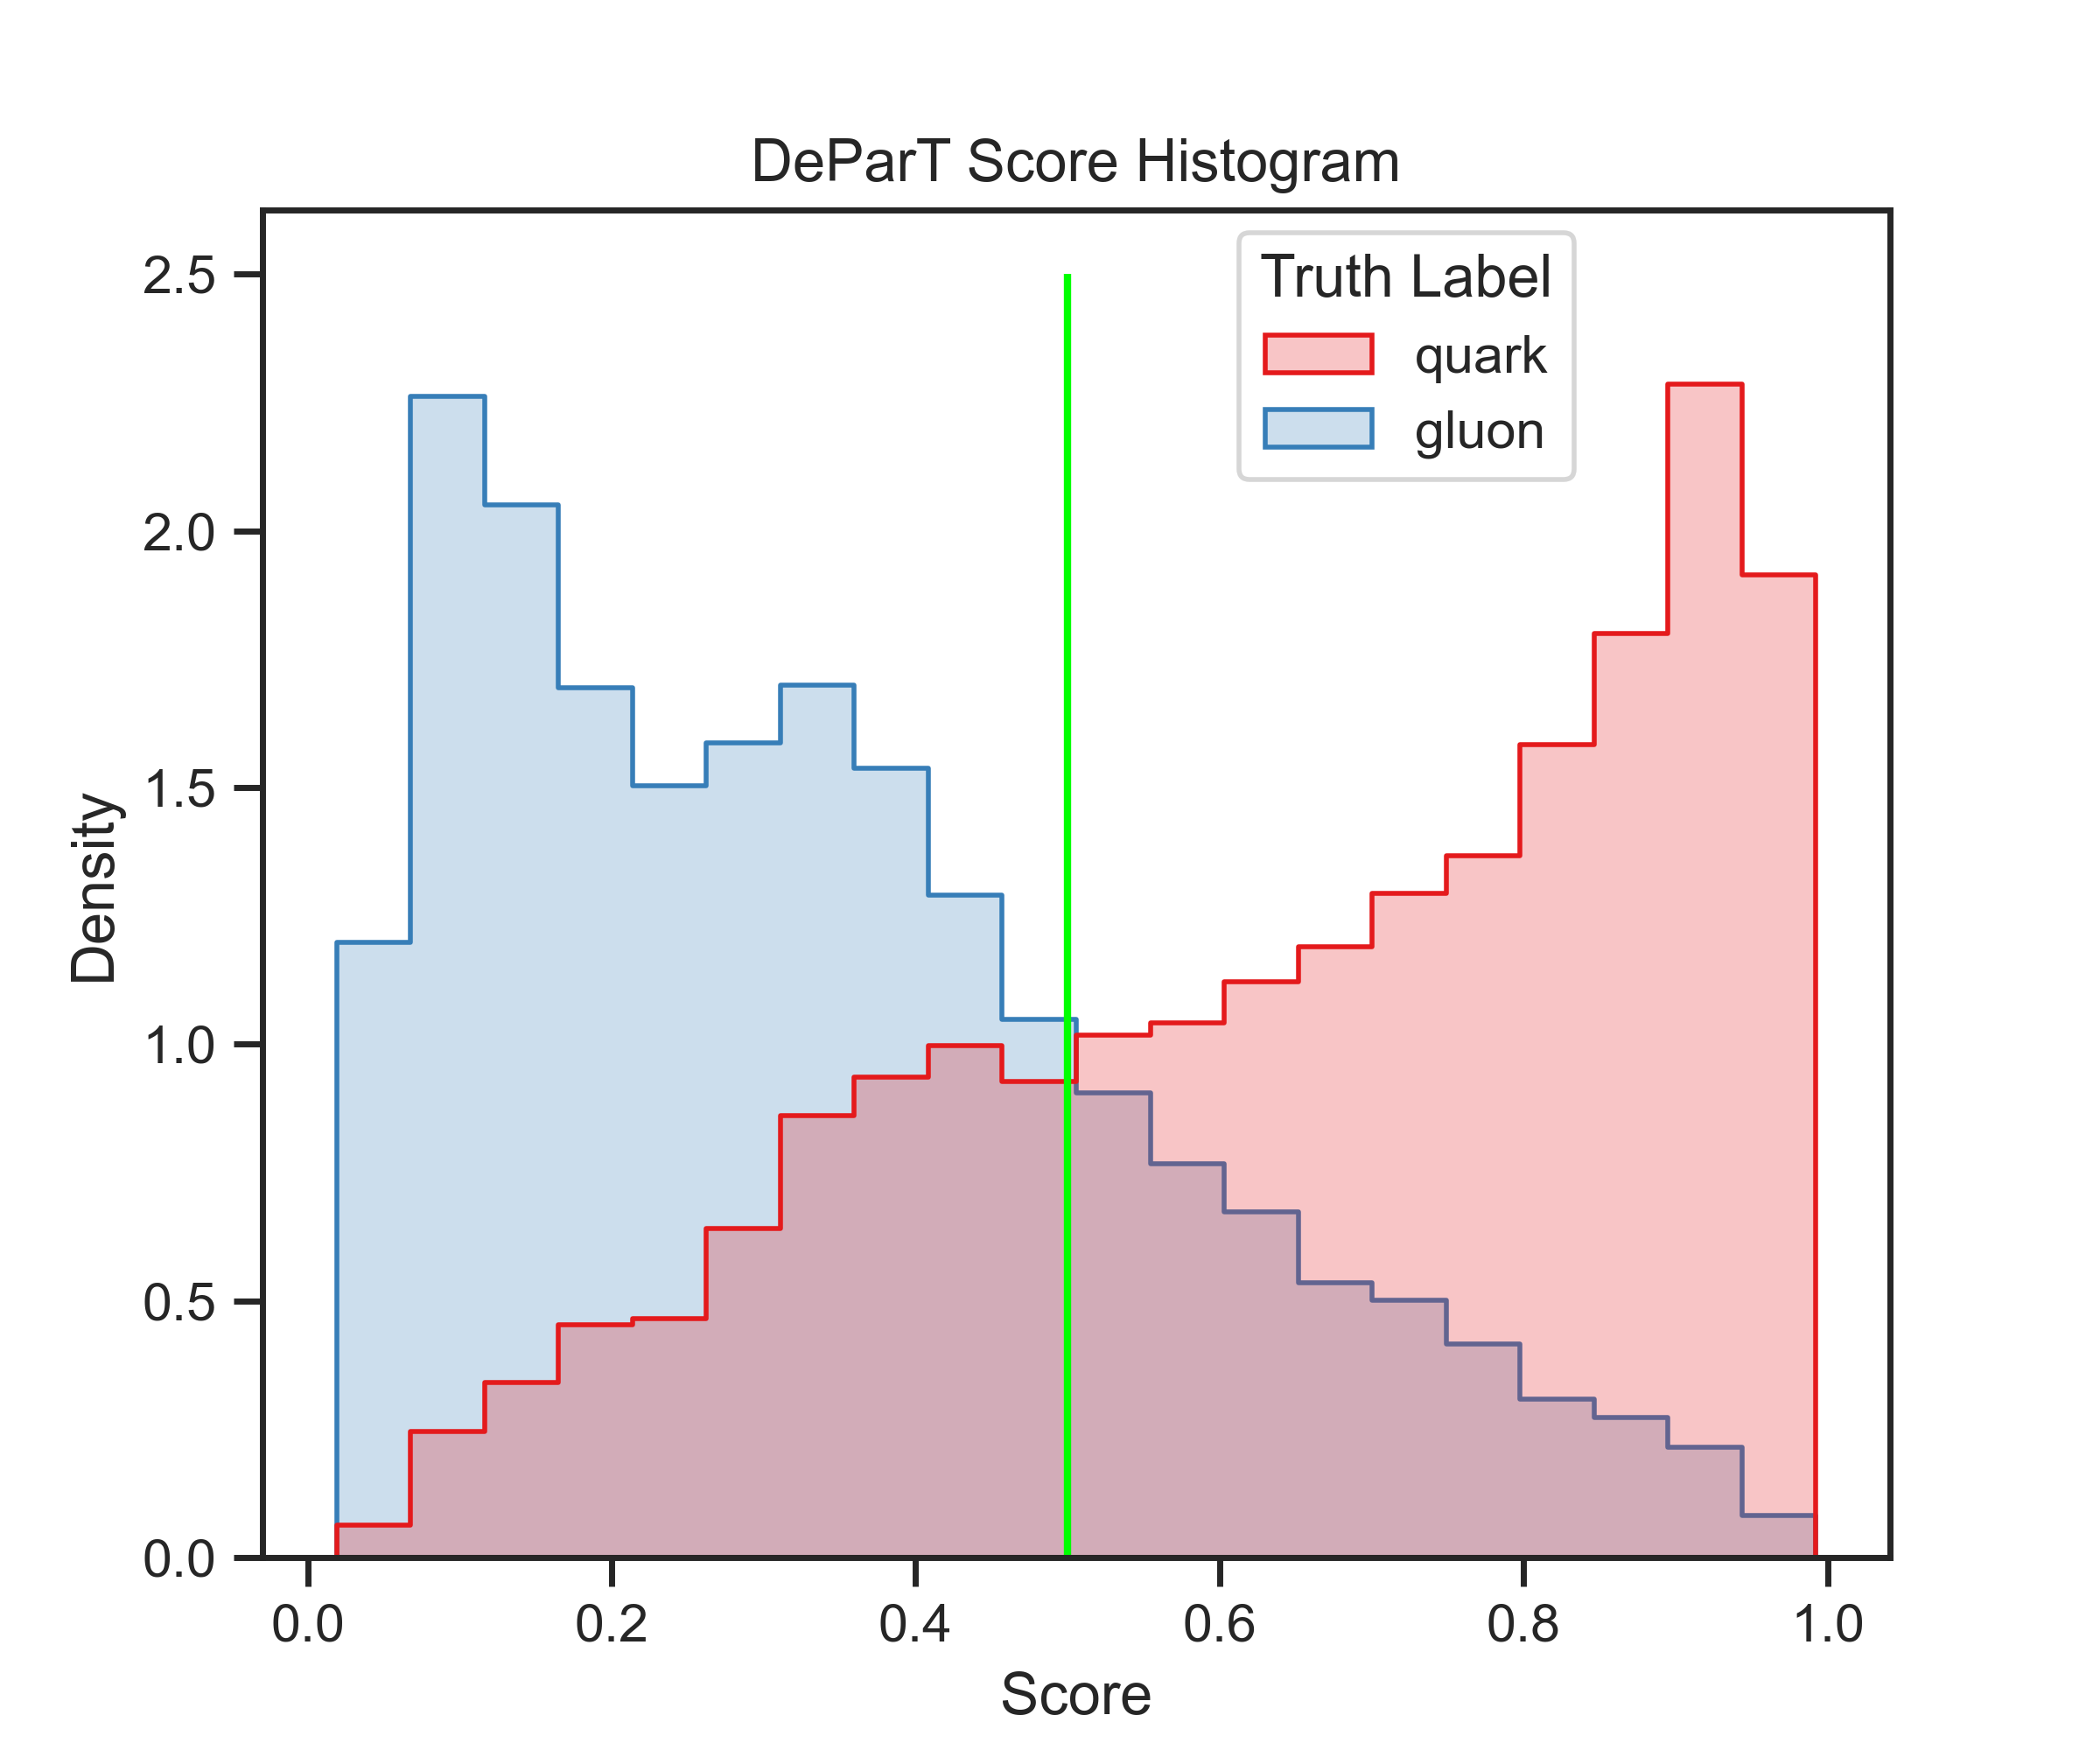
\includegraphics[width=1\textwidth]{src/plots/results/score/depart.png}
		\caption{DeParT}
		\label{fig:app_score_depart}
	\end{subfigure}
	\begin{subfigure}[t]{0.49\textwidth}
		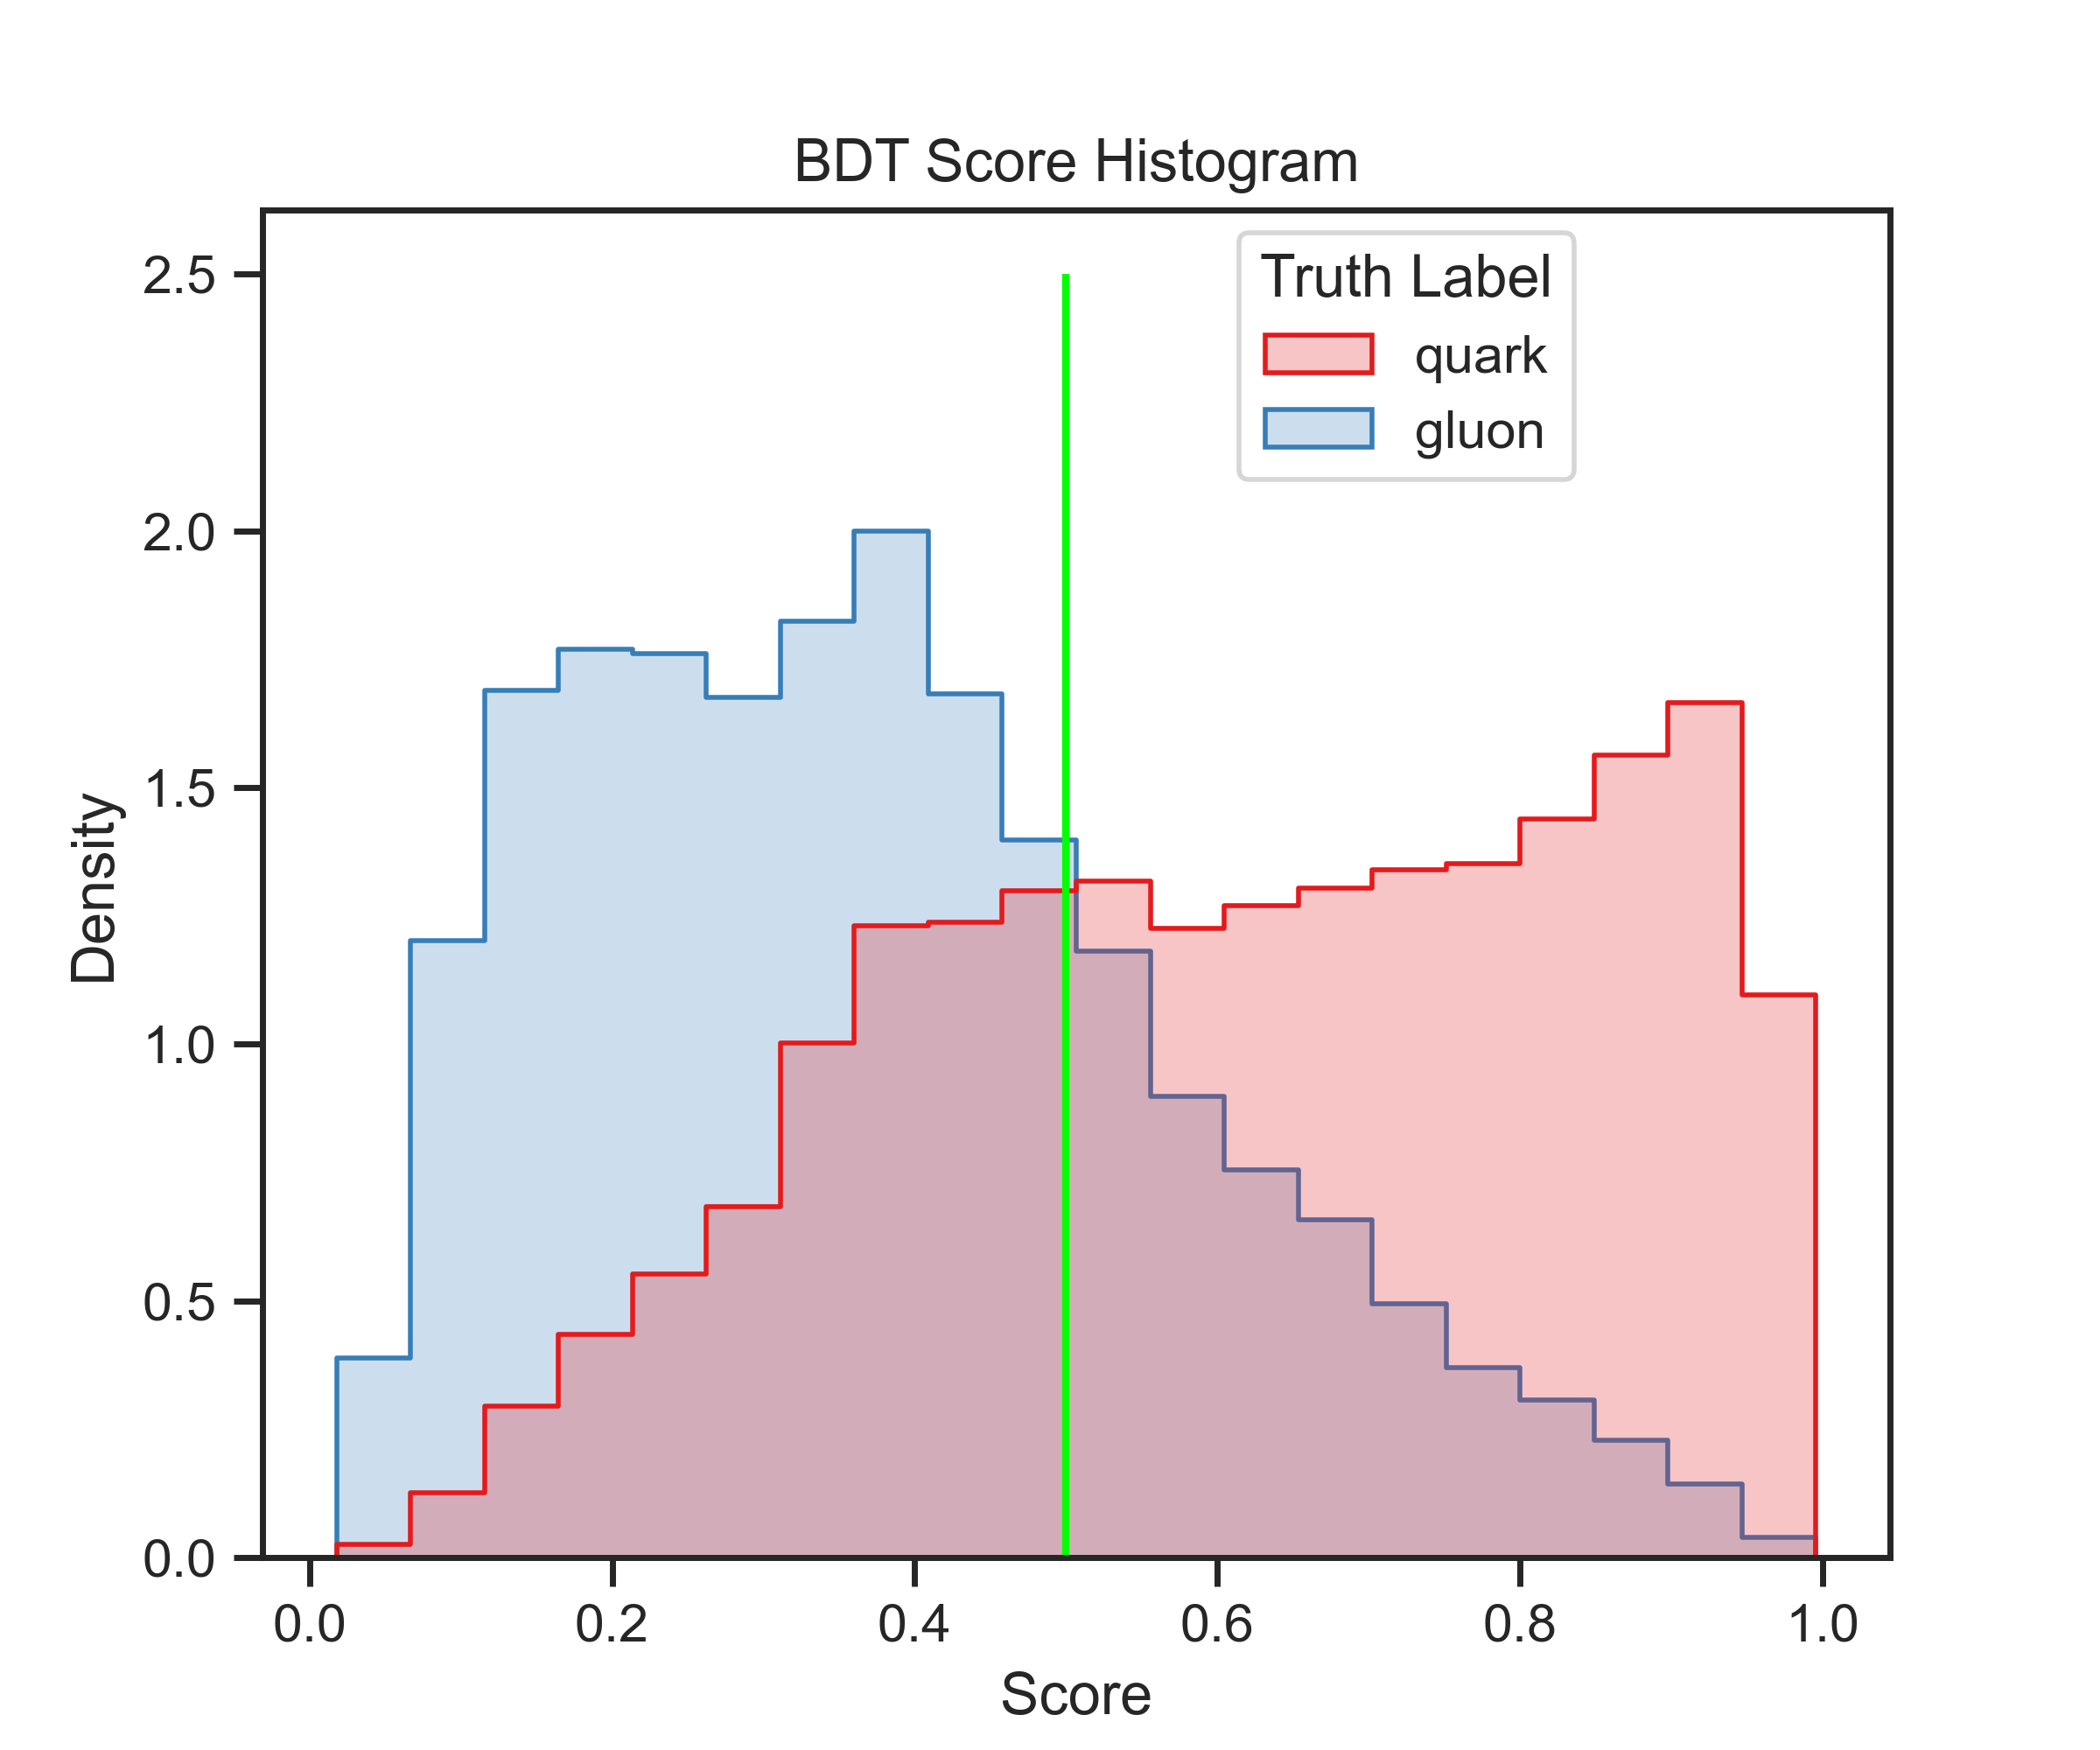
\includegraphics[width=1\textwidth]{src/plots/results/score/bdt.png}
		\caption{BDT}
		\label{fig:app_score_bdt}
	\end{subfigure}
	\begin{subfigure}[t]{0.49\textwidth}
		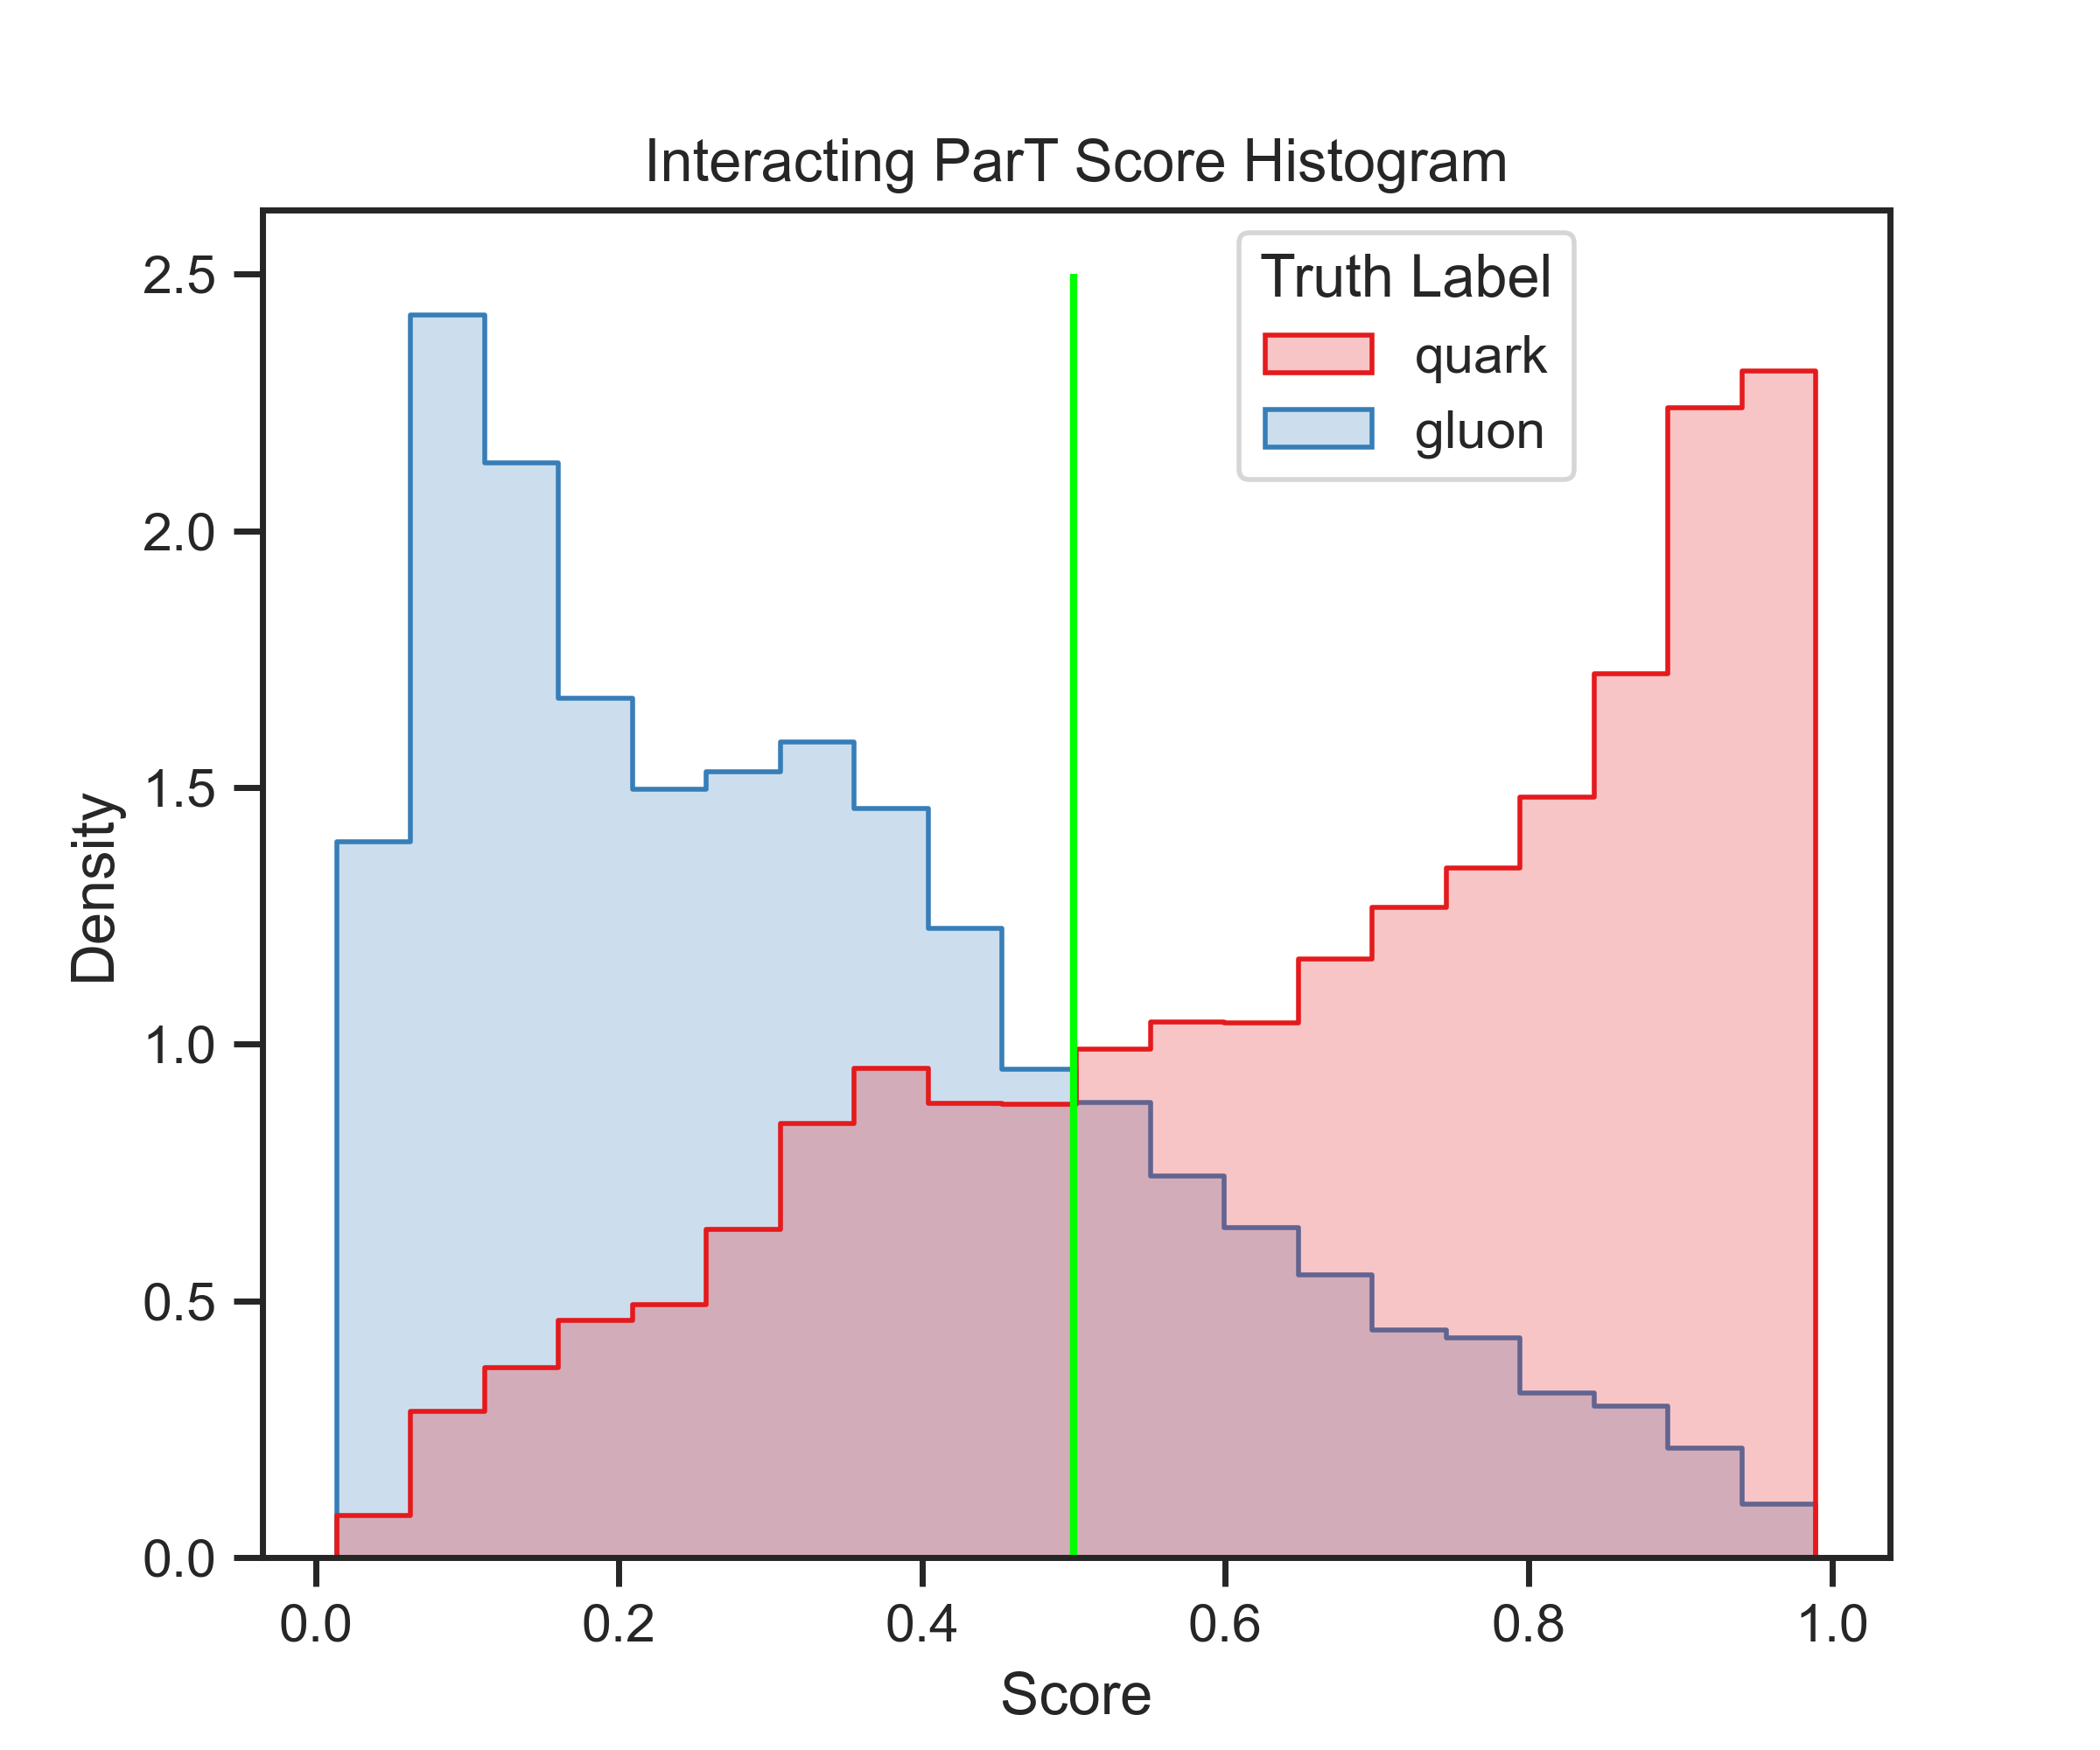
\includegraphics[width=1\textwidth]{src/plots/results/score/interacting_part.png}
		\caption{Interacting ParT}
		\label{fig:app_score_interacting_part}
	\end{subfigure}
	\begin{subfigure}[t]{0.49\textwidth}
		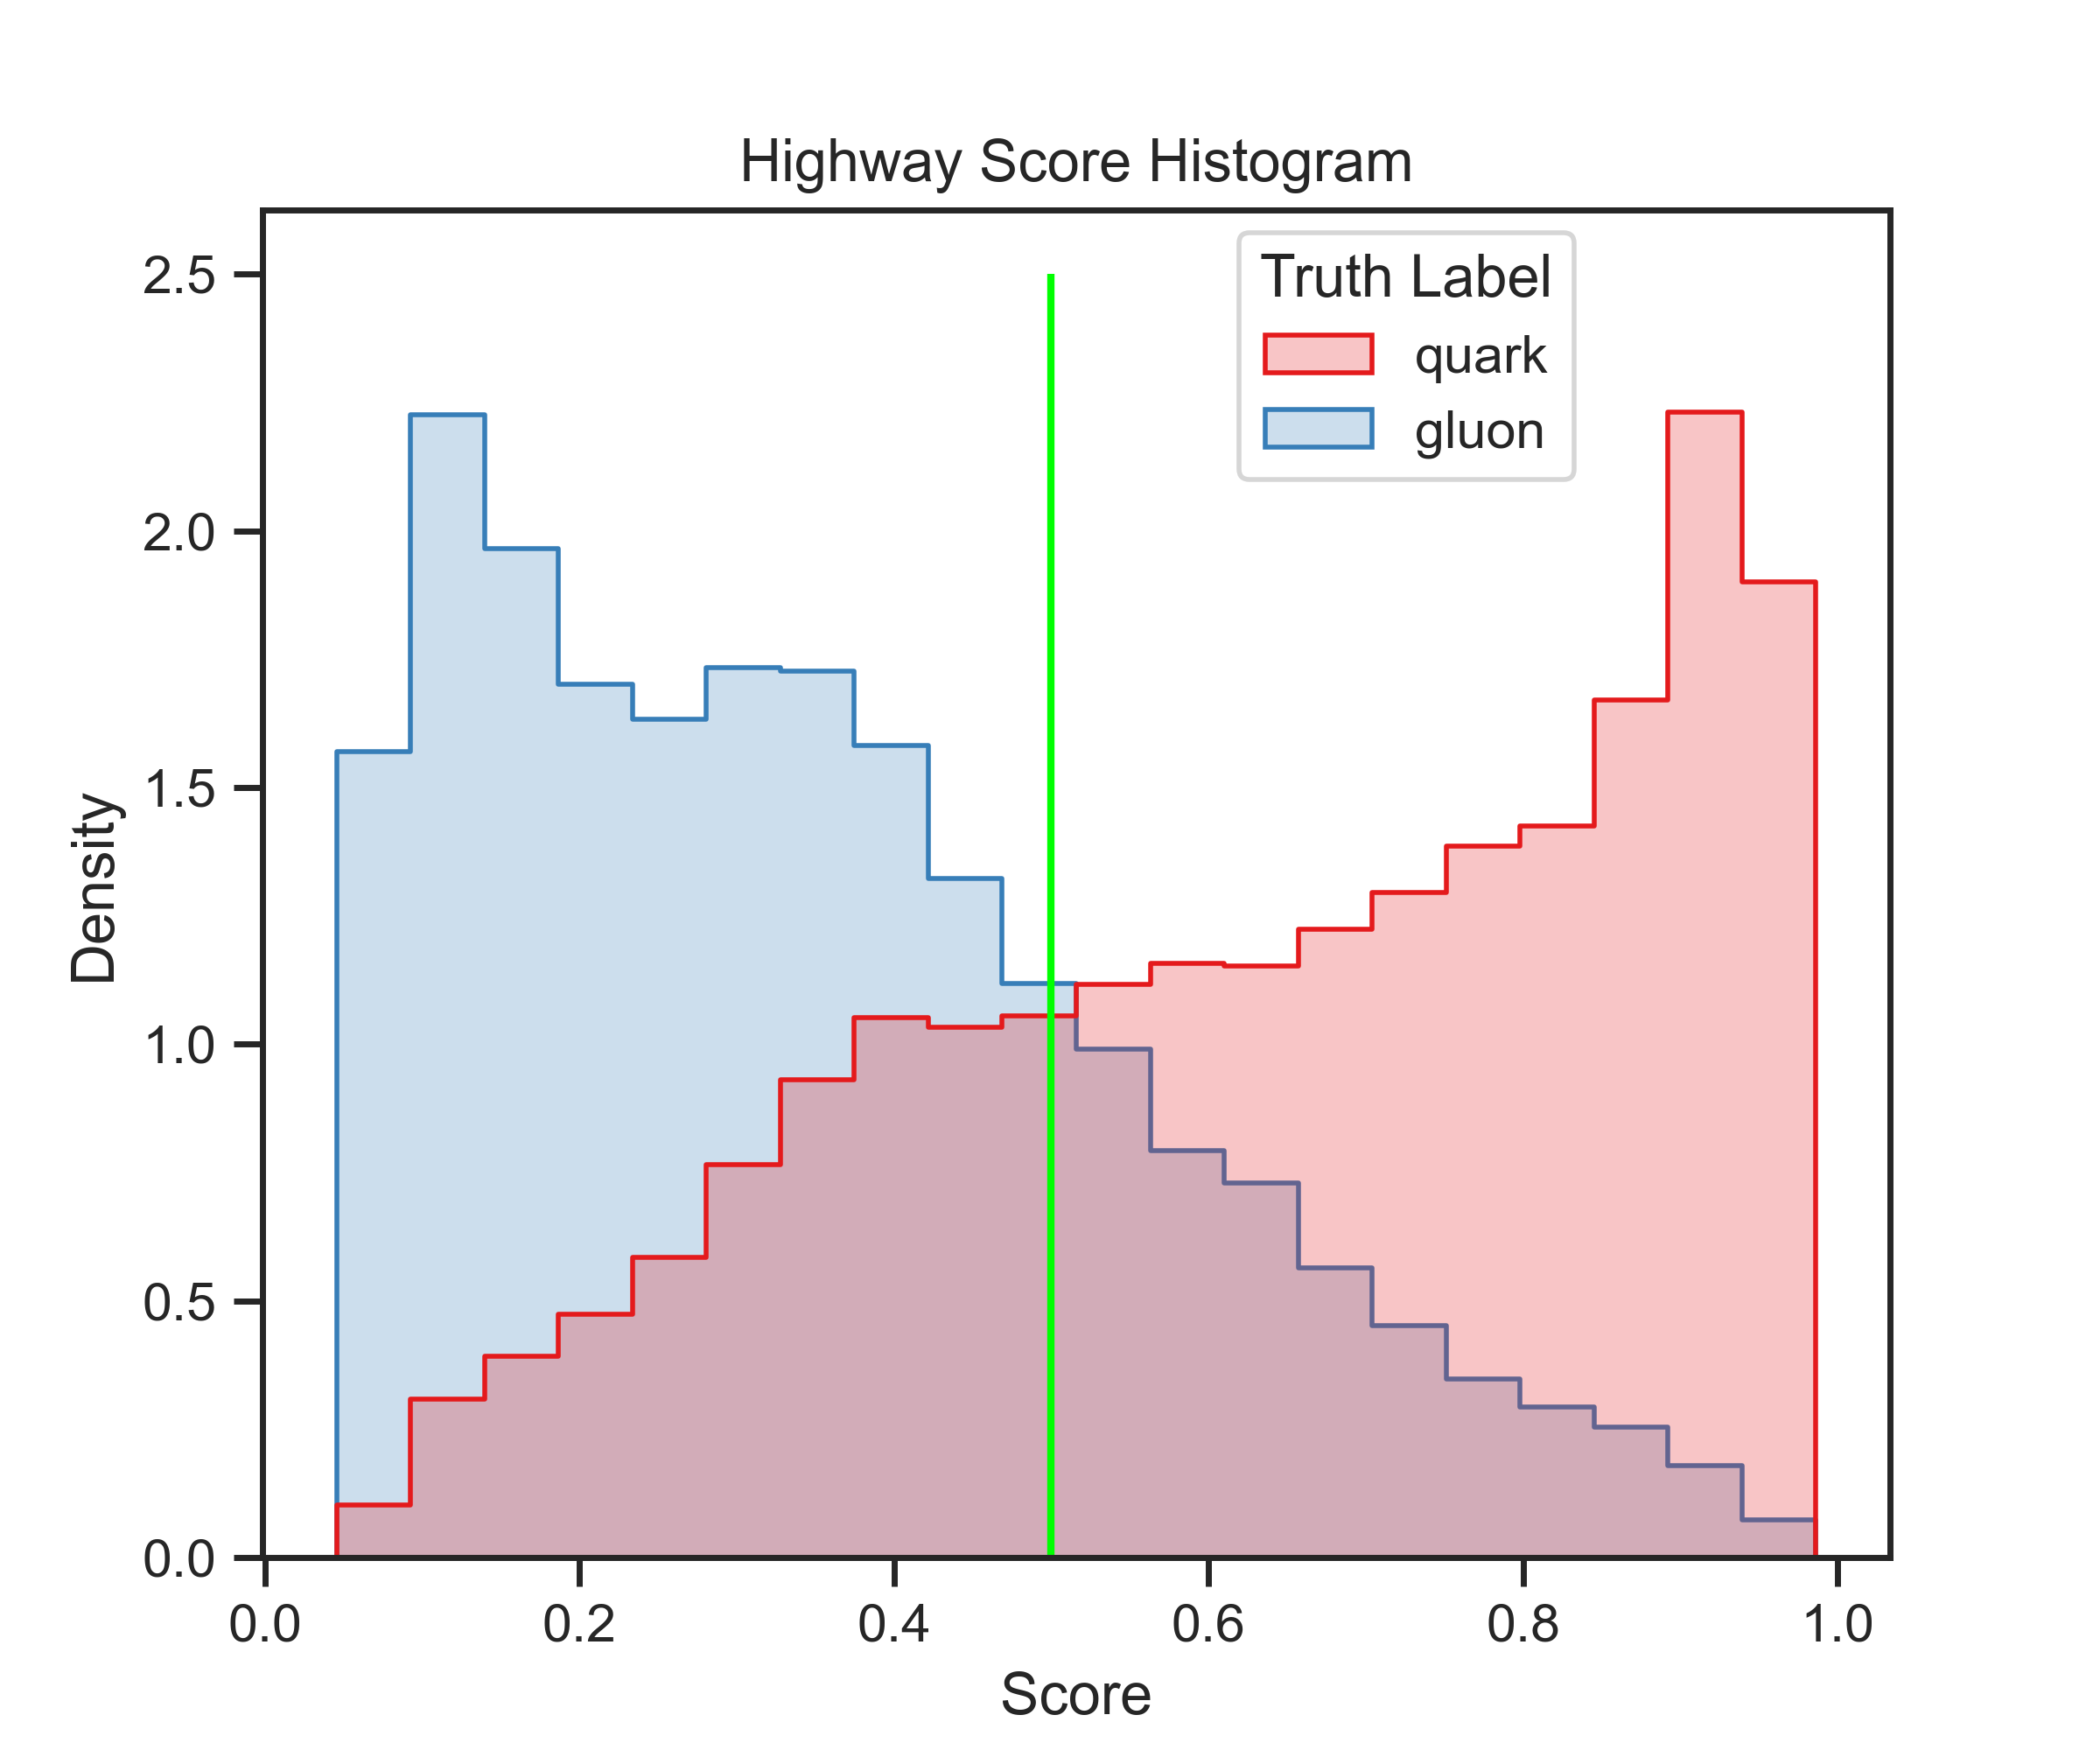
\includegraphics[width=1\textwidth]{src/plots/results/score/highway.png}
		\caption{Highway}
		\label{fig:app_score_highway}
	\end{subfigure}
\caption{Confusion Matricies}
\label{fig:app_score_-1-3}
\end{figure}

\begin{figure}[!htb]
	\centering
	\begin{subfigure}[t]{0.49\textwidth}
		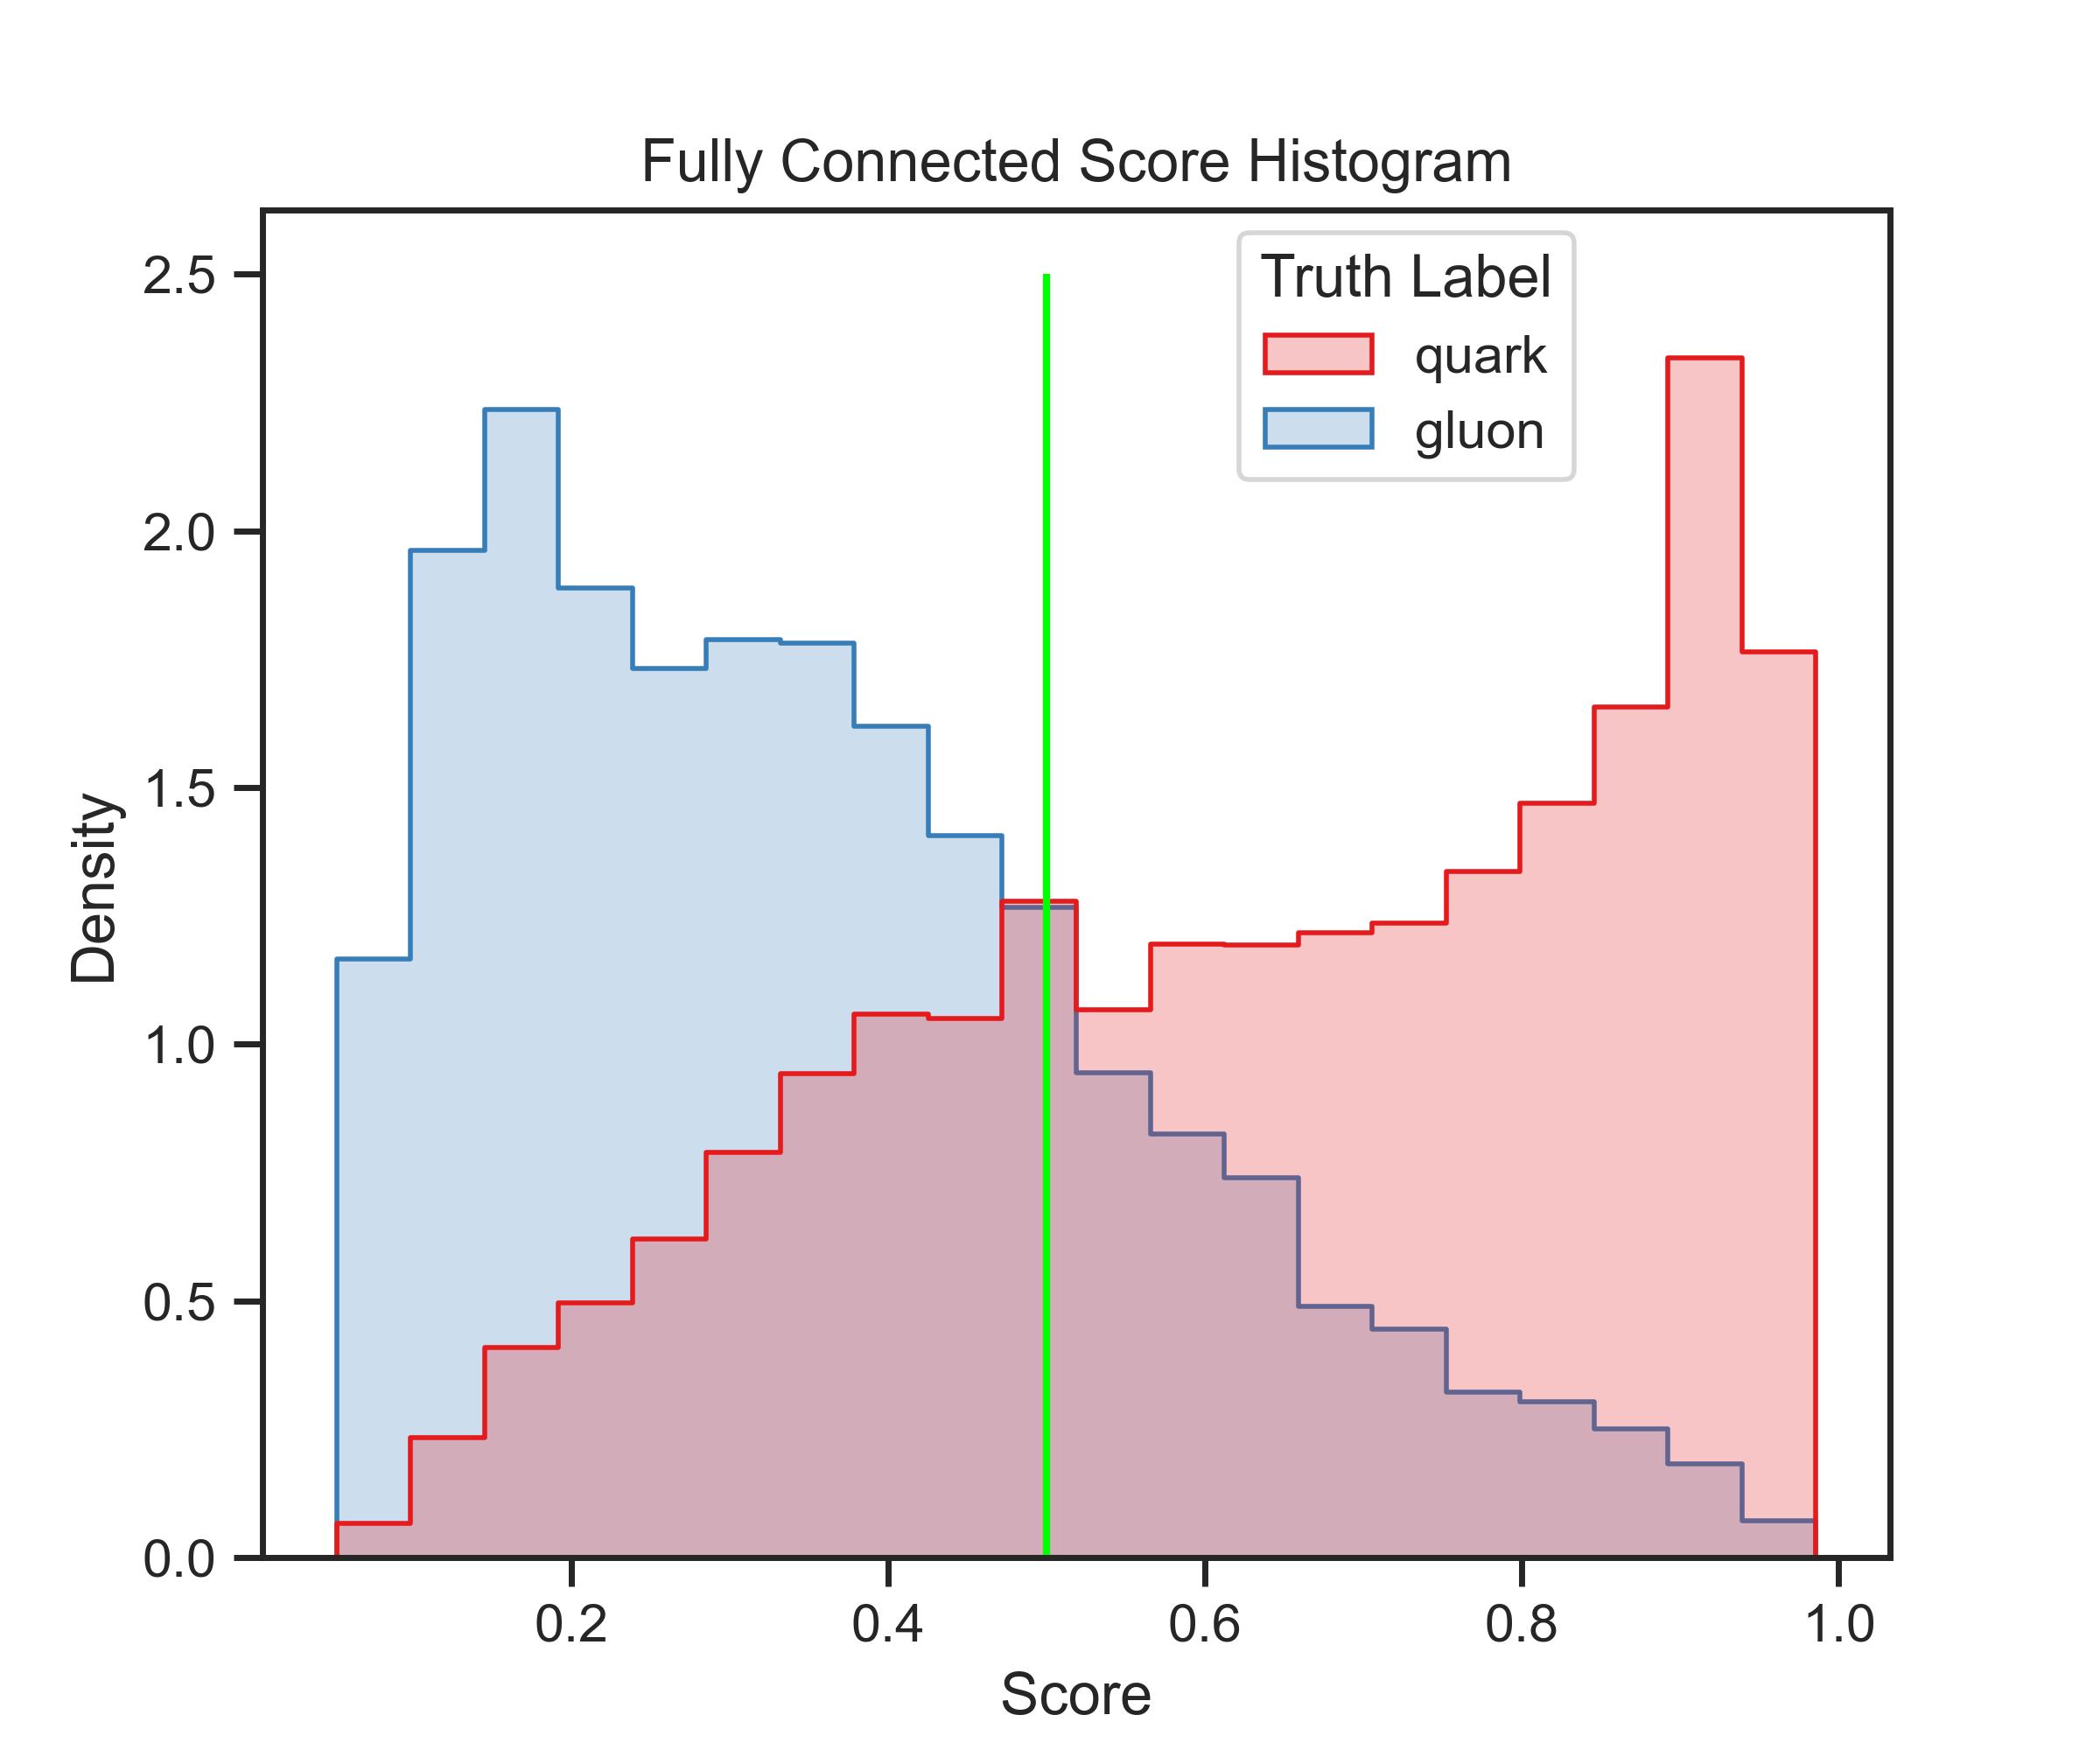
\includegraphics[width=1\textwidth]{src/plots/results/score/fc.png}
		\caption{Fully Connected}
		\label{fig:app_score_fc}
	\end{subfigure}
	\begin{subfigure}[t]{0.49\textwidth}
		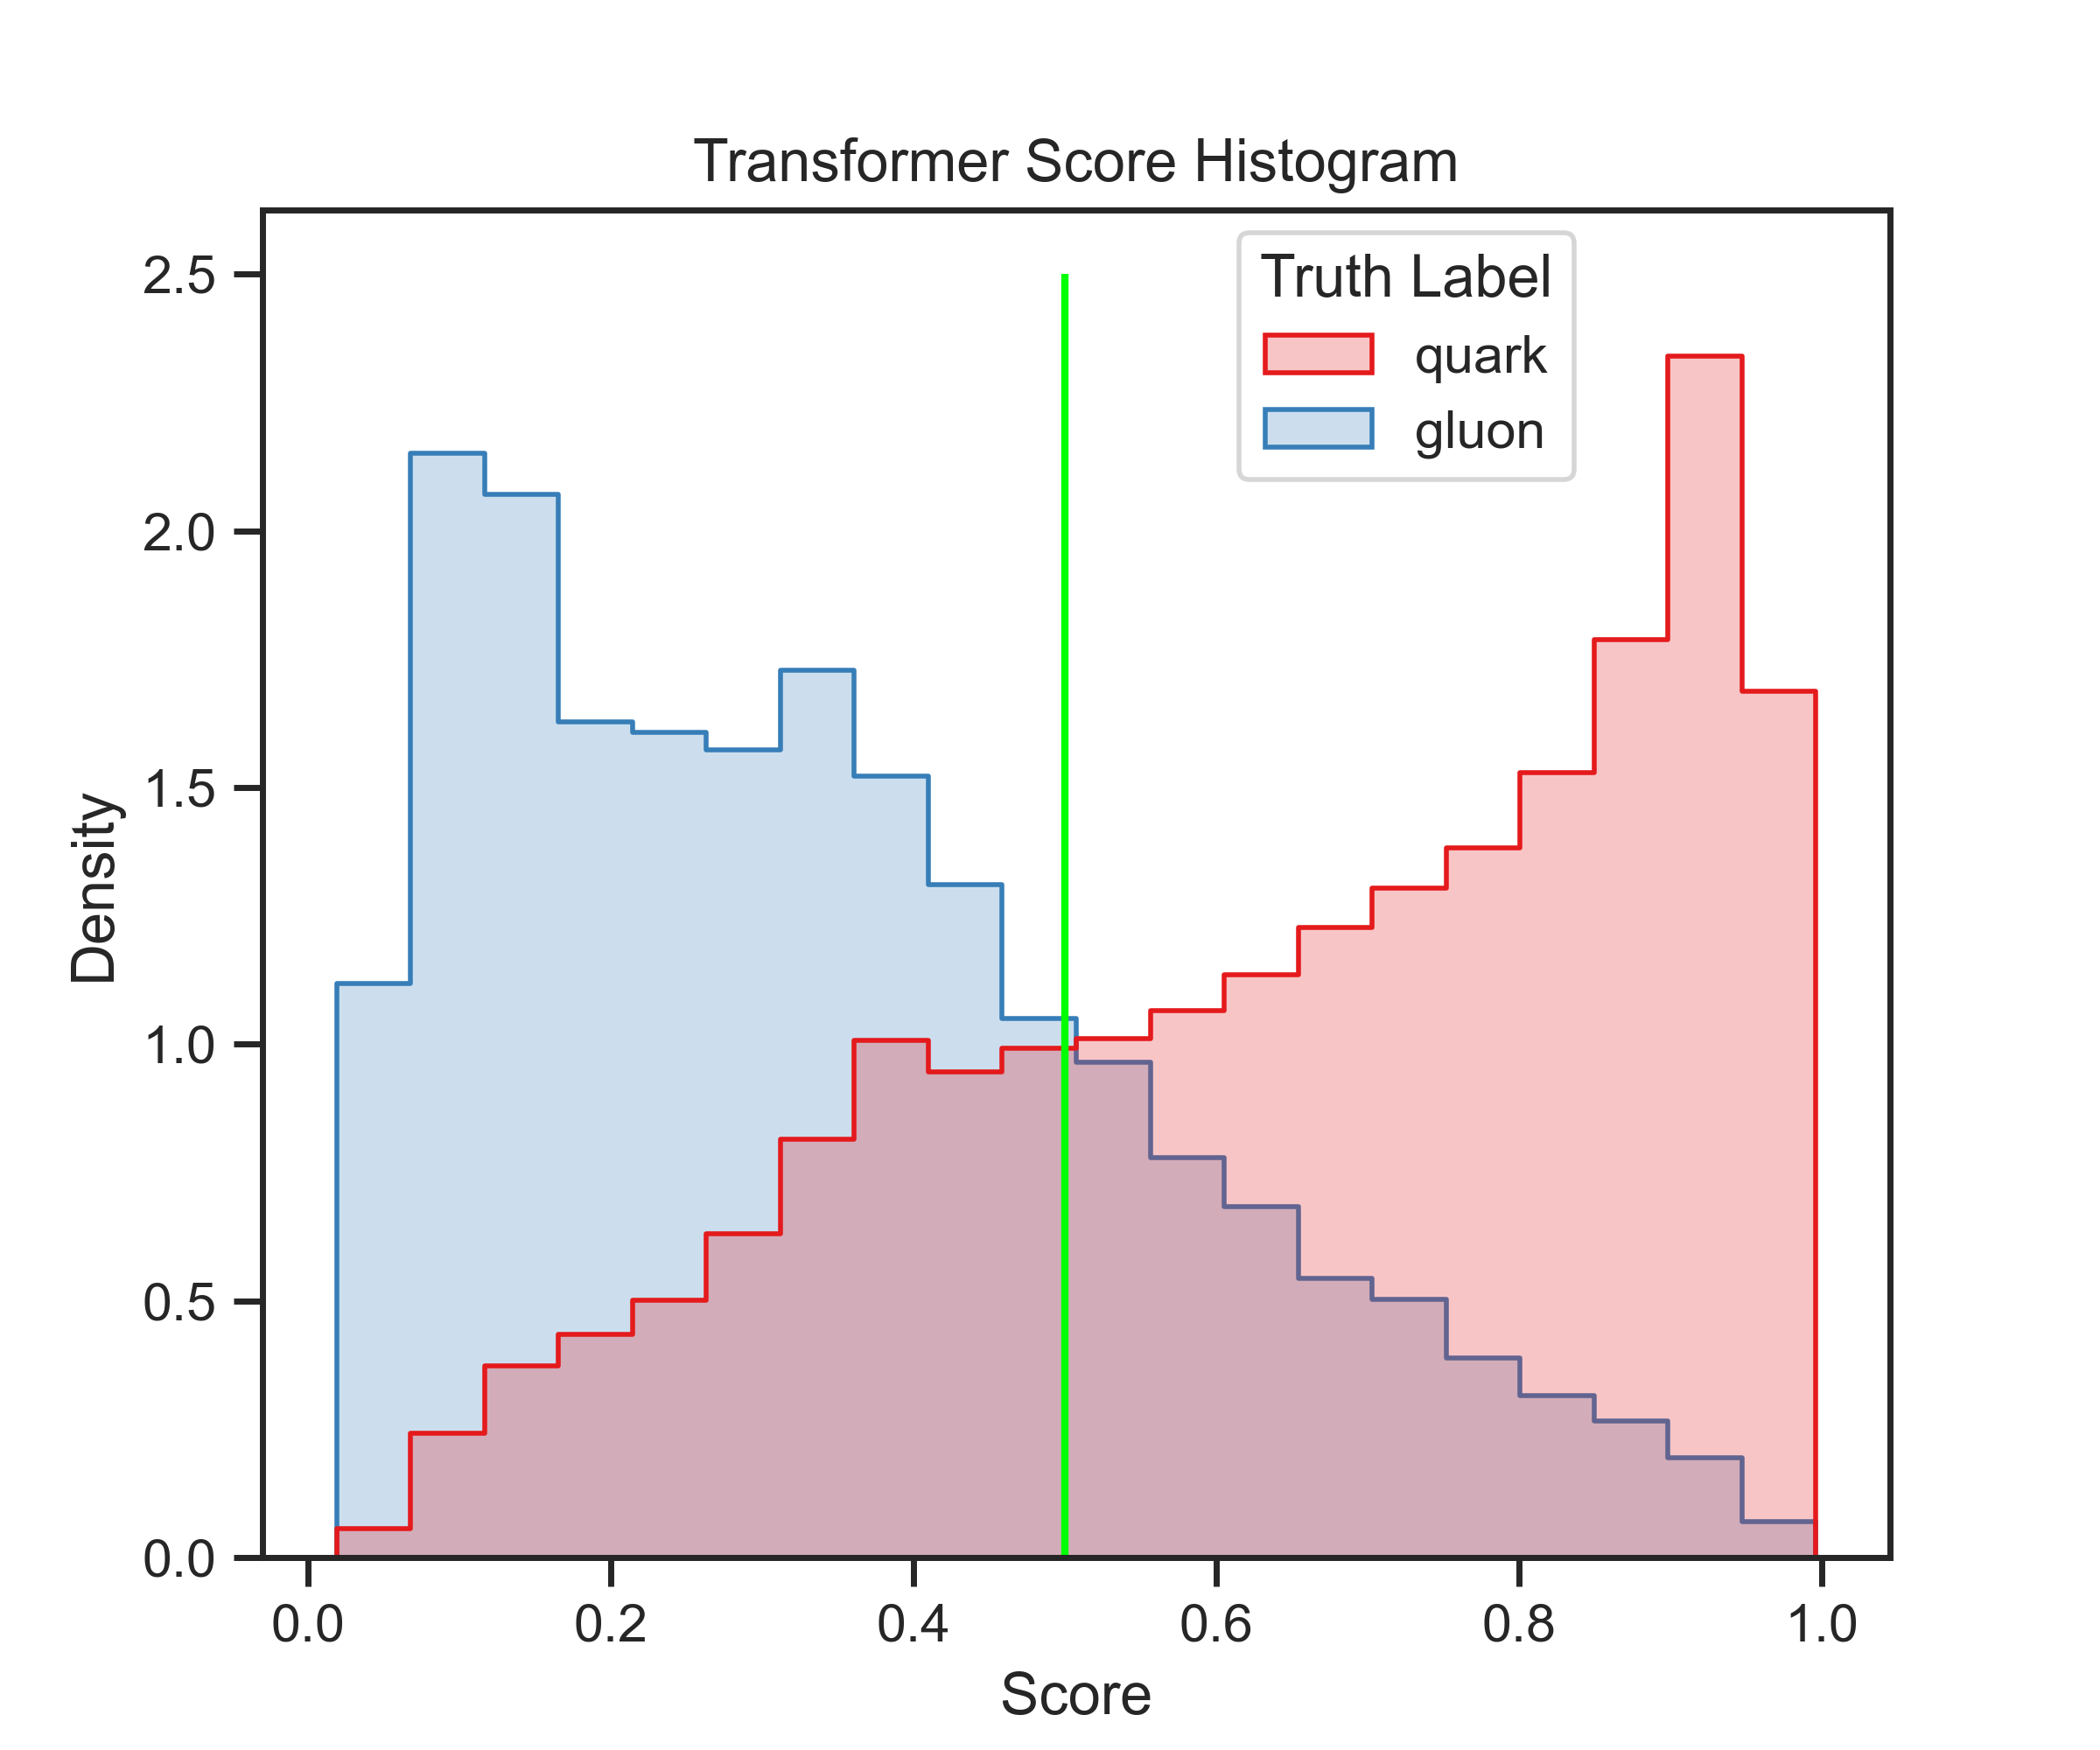
\includegraphics[width=1\textwidth]{src/plots/results/score/transformer.png}
		\caption{Transformer}
		\label{fig:app_score_transformer}
	\end{subfigure}
	\begin{subfigure}[t]{0.49\textwidth}
		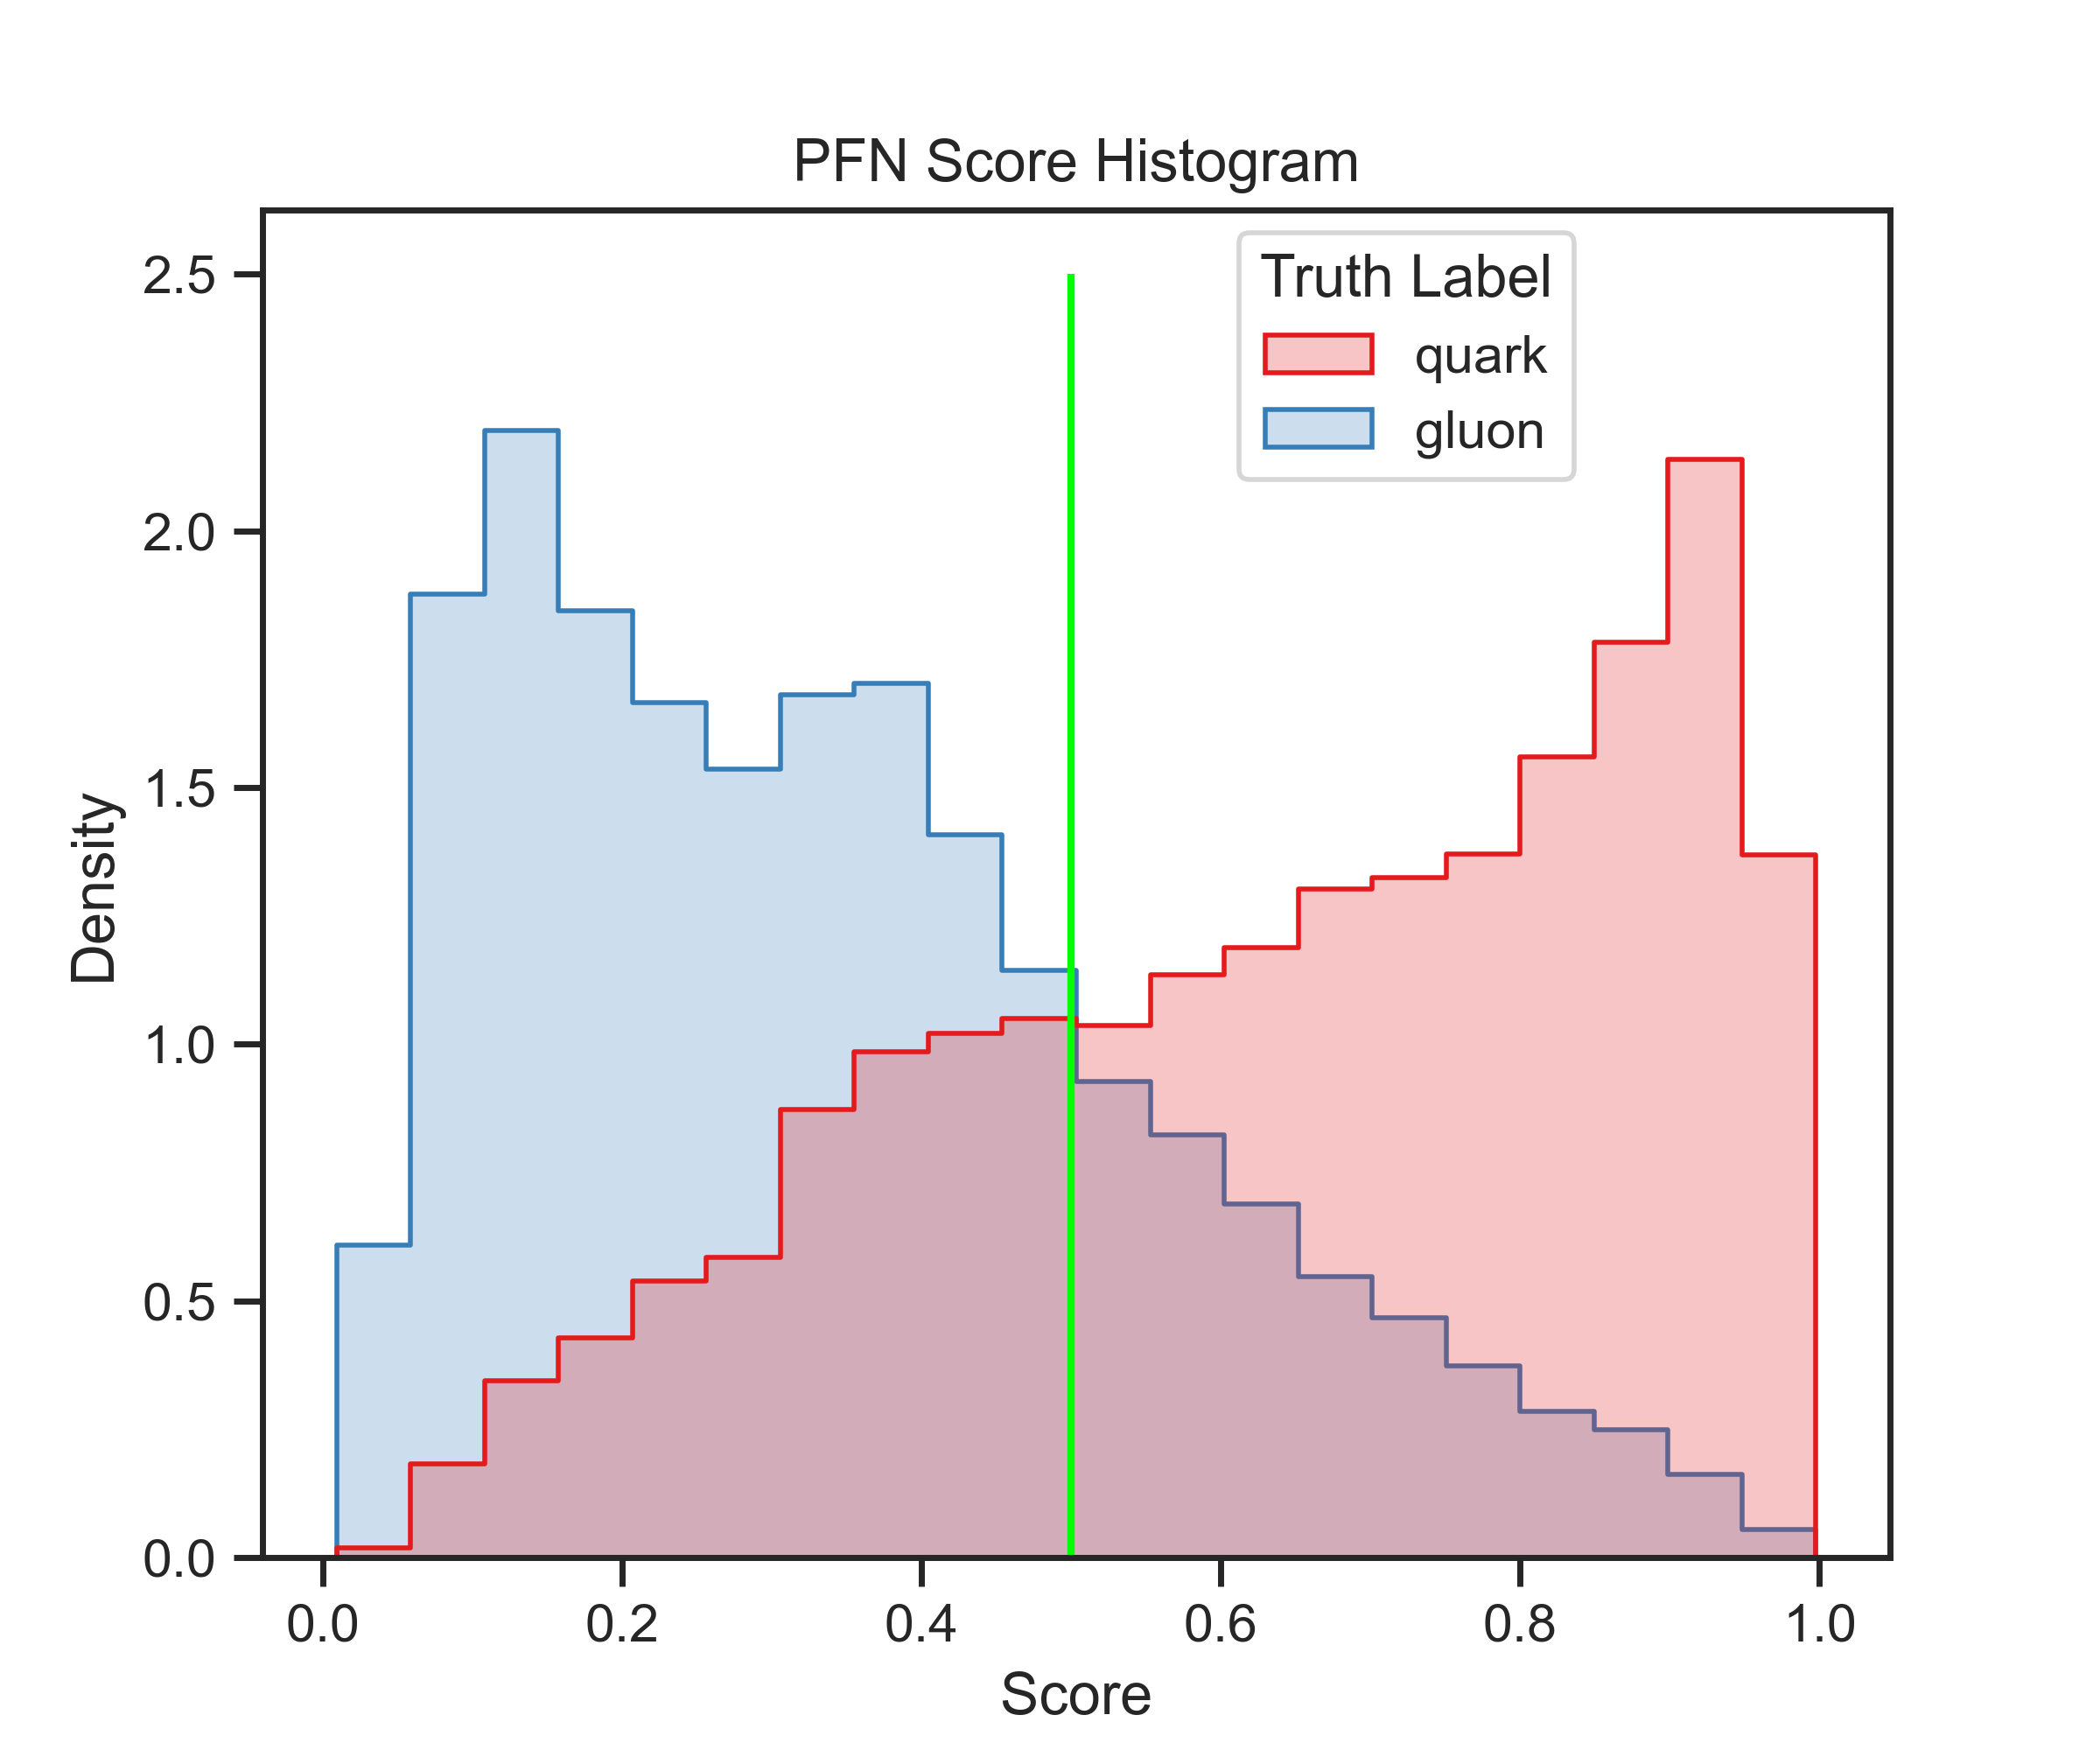
\includegraphics[width=1\textwidth]{src/plots/results/score/pfn.png}
		\caption{PFN}
		\label{fig:app_score_pfn}
	\end{subfigure}
	\begin{subfigure}[t]{0.49\textwidth}
		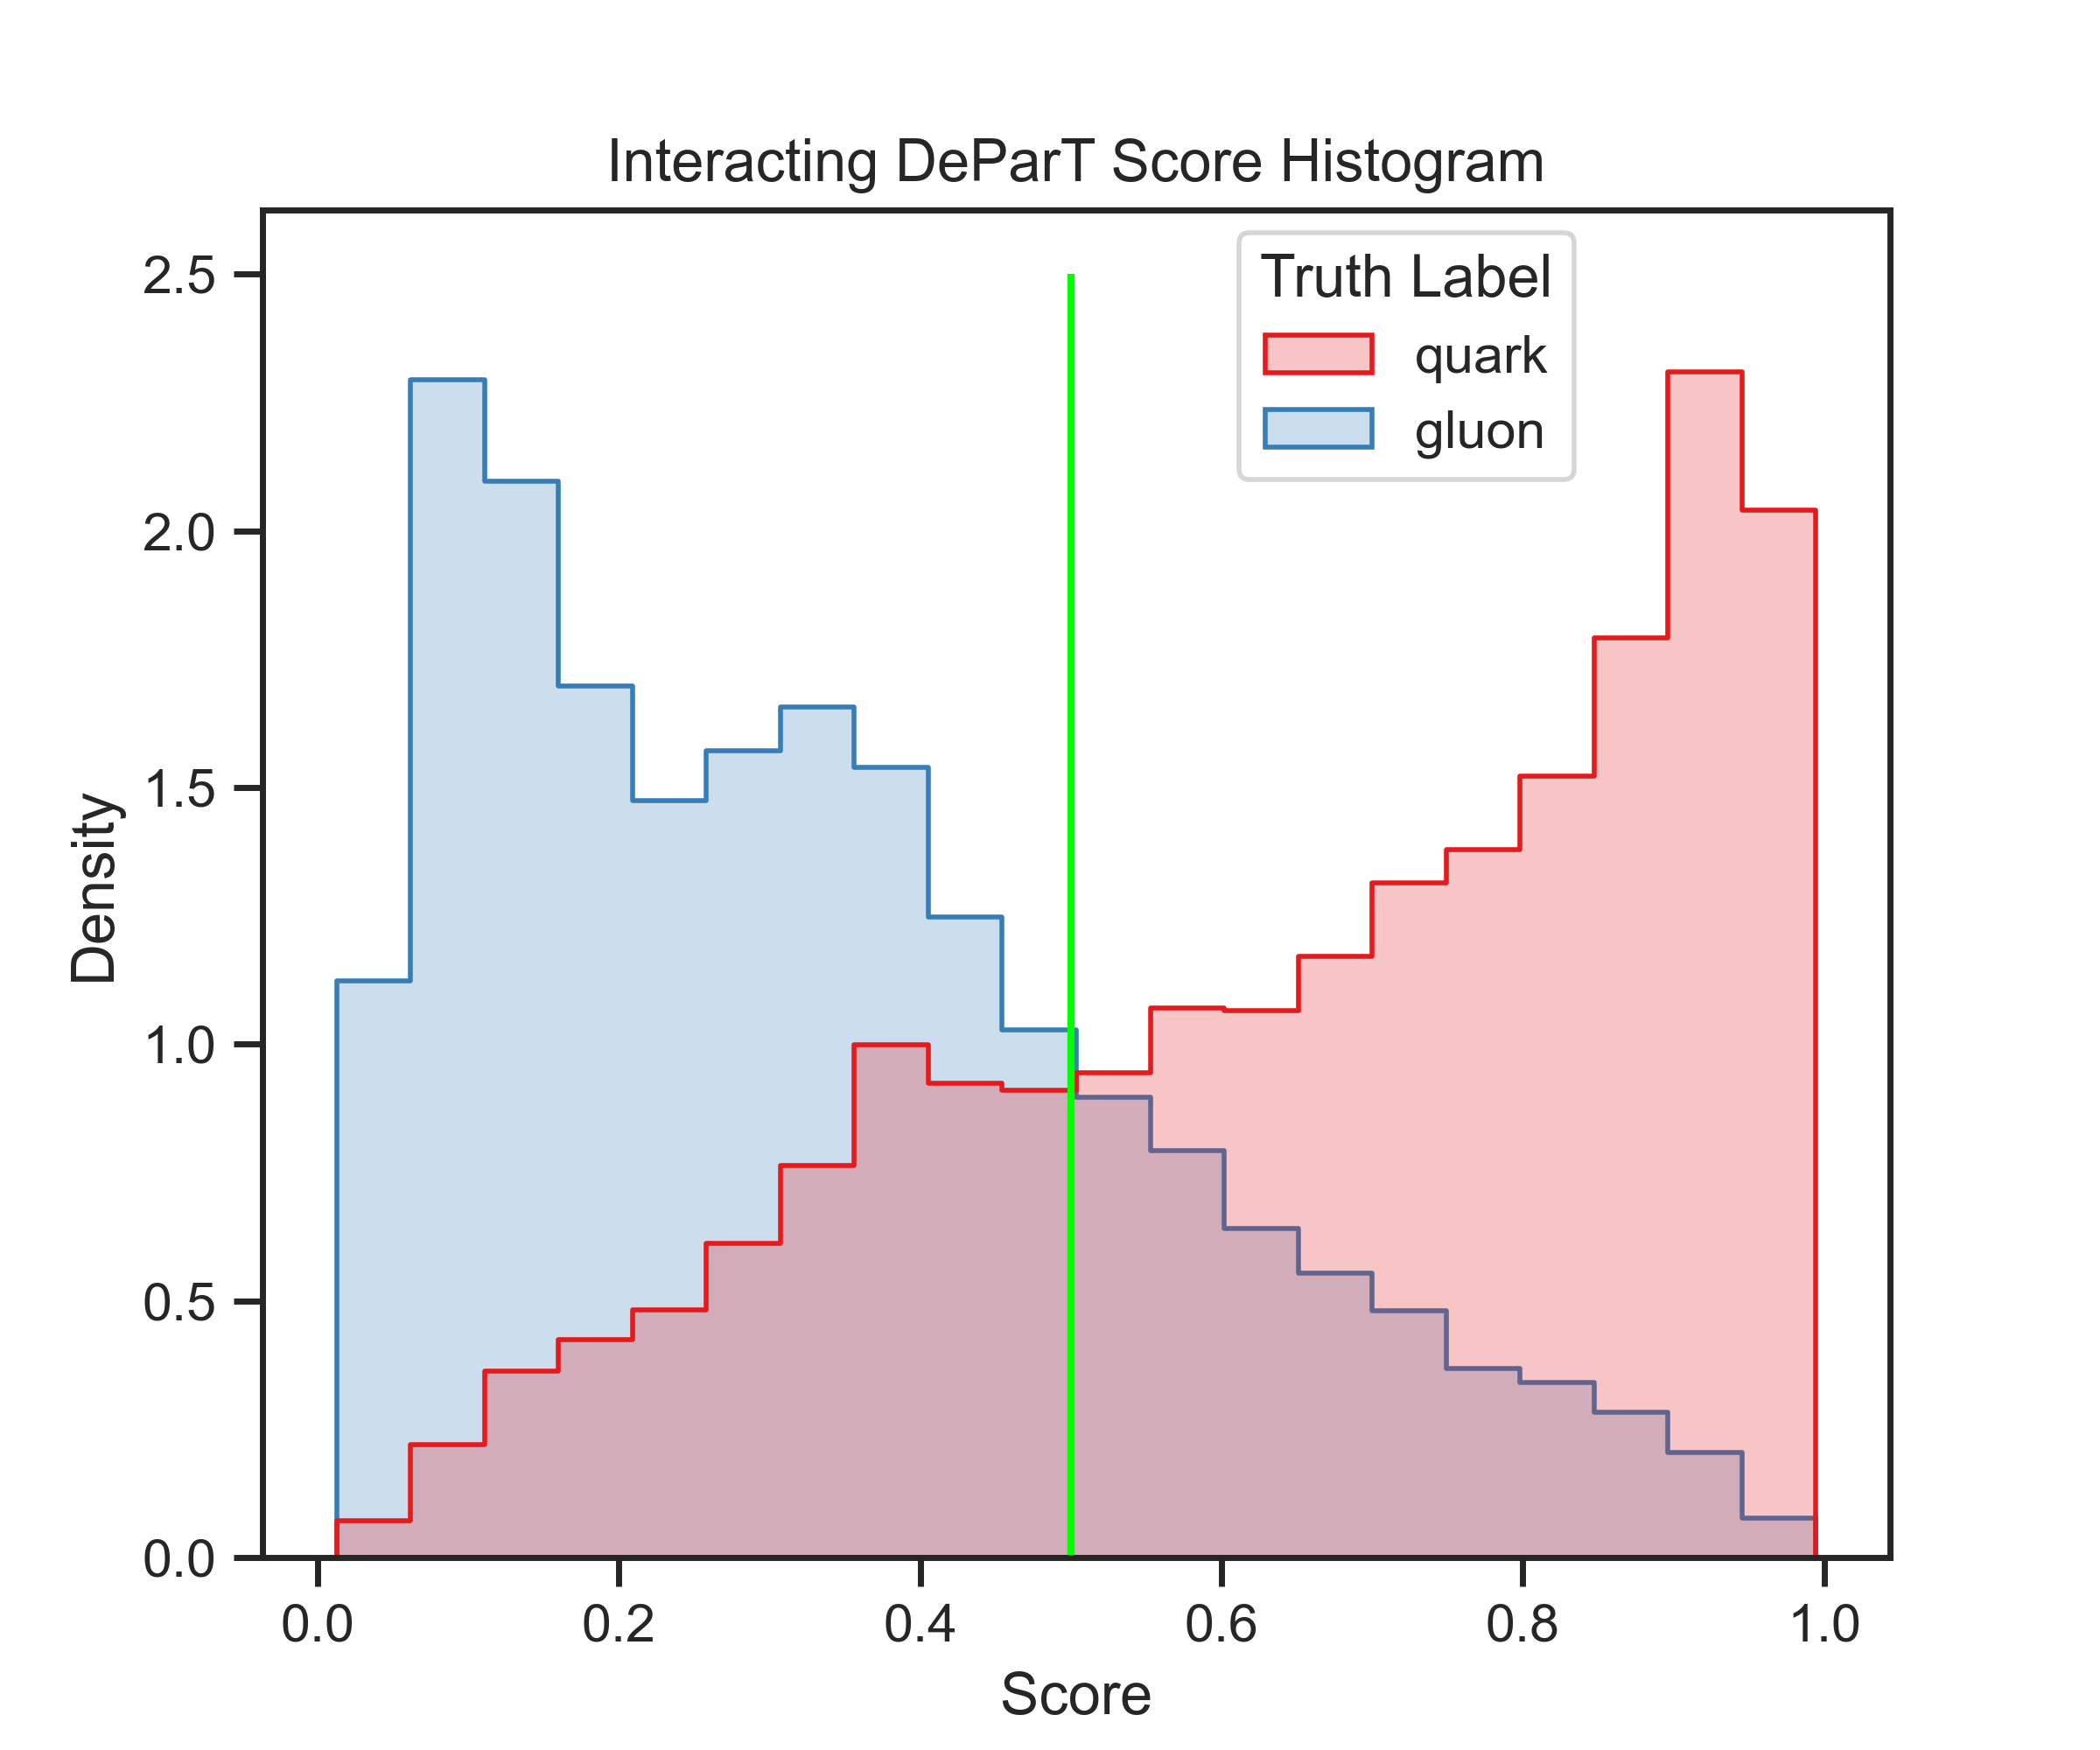
\includegraphics[width=1\textwidth]{src/plots/results/score/interacting_depart.png}
		\caption{Interacting DeParT}
		\label{fig:app_score_interacting_depart}
	\end{subfigure}
	\begin{subfigure}[t]{0.49\textwidth}
		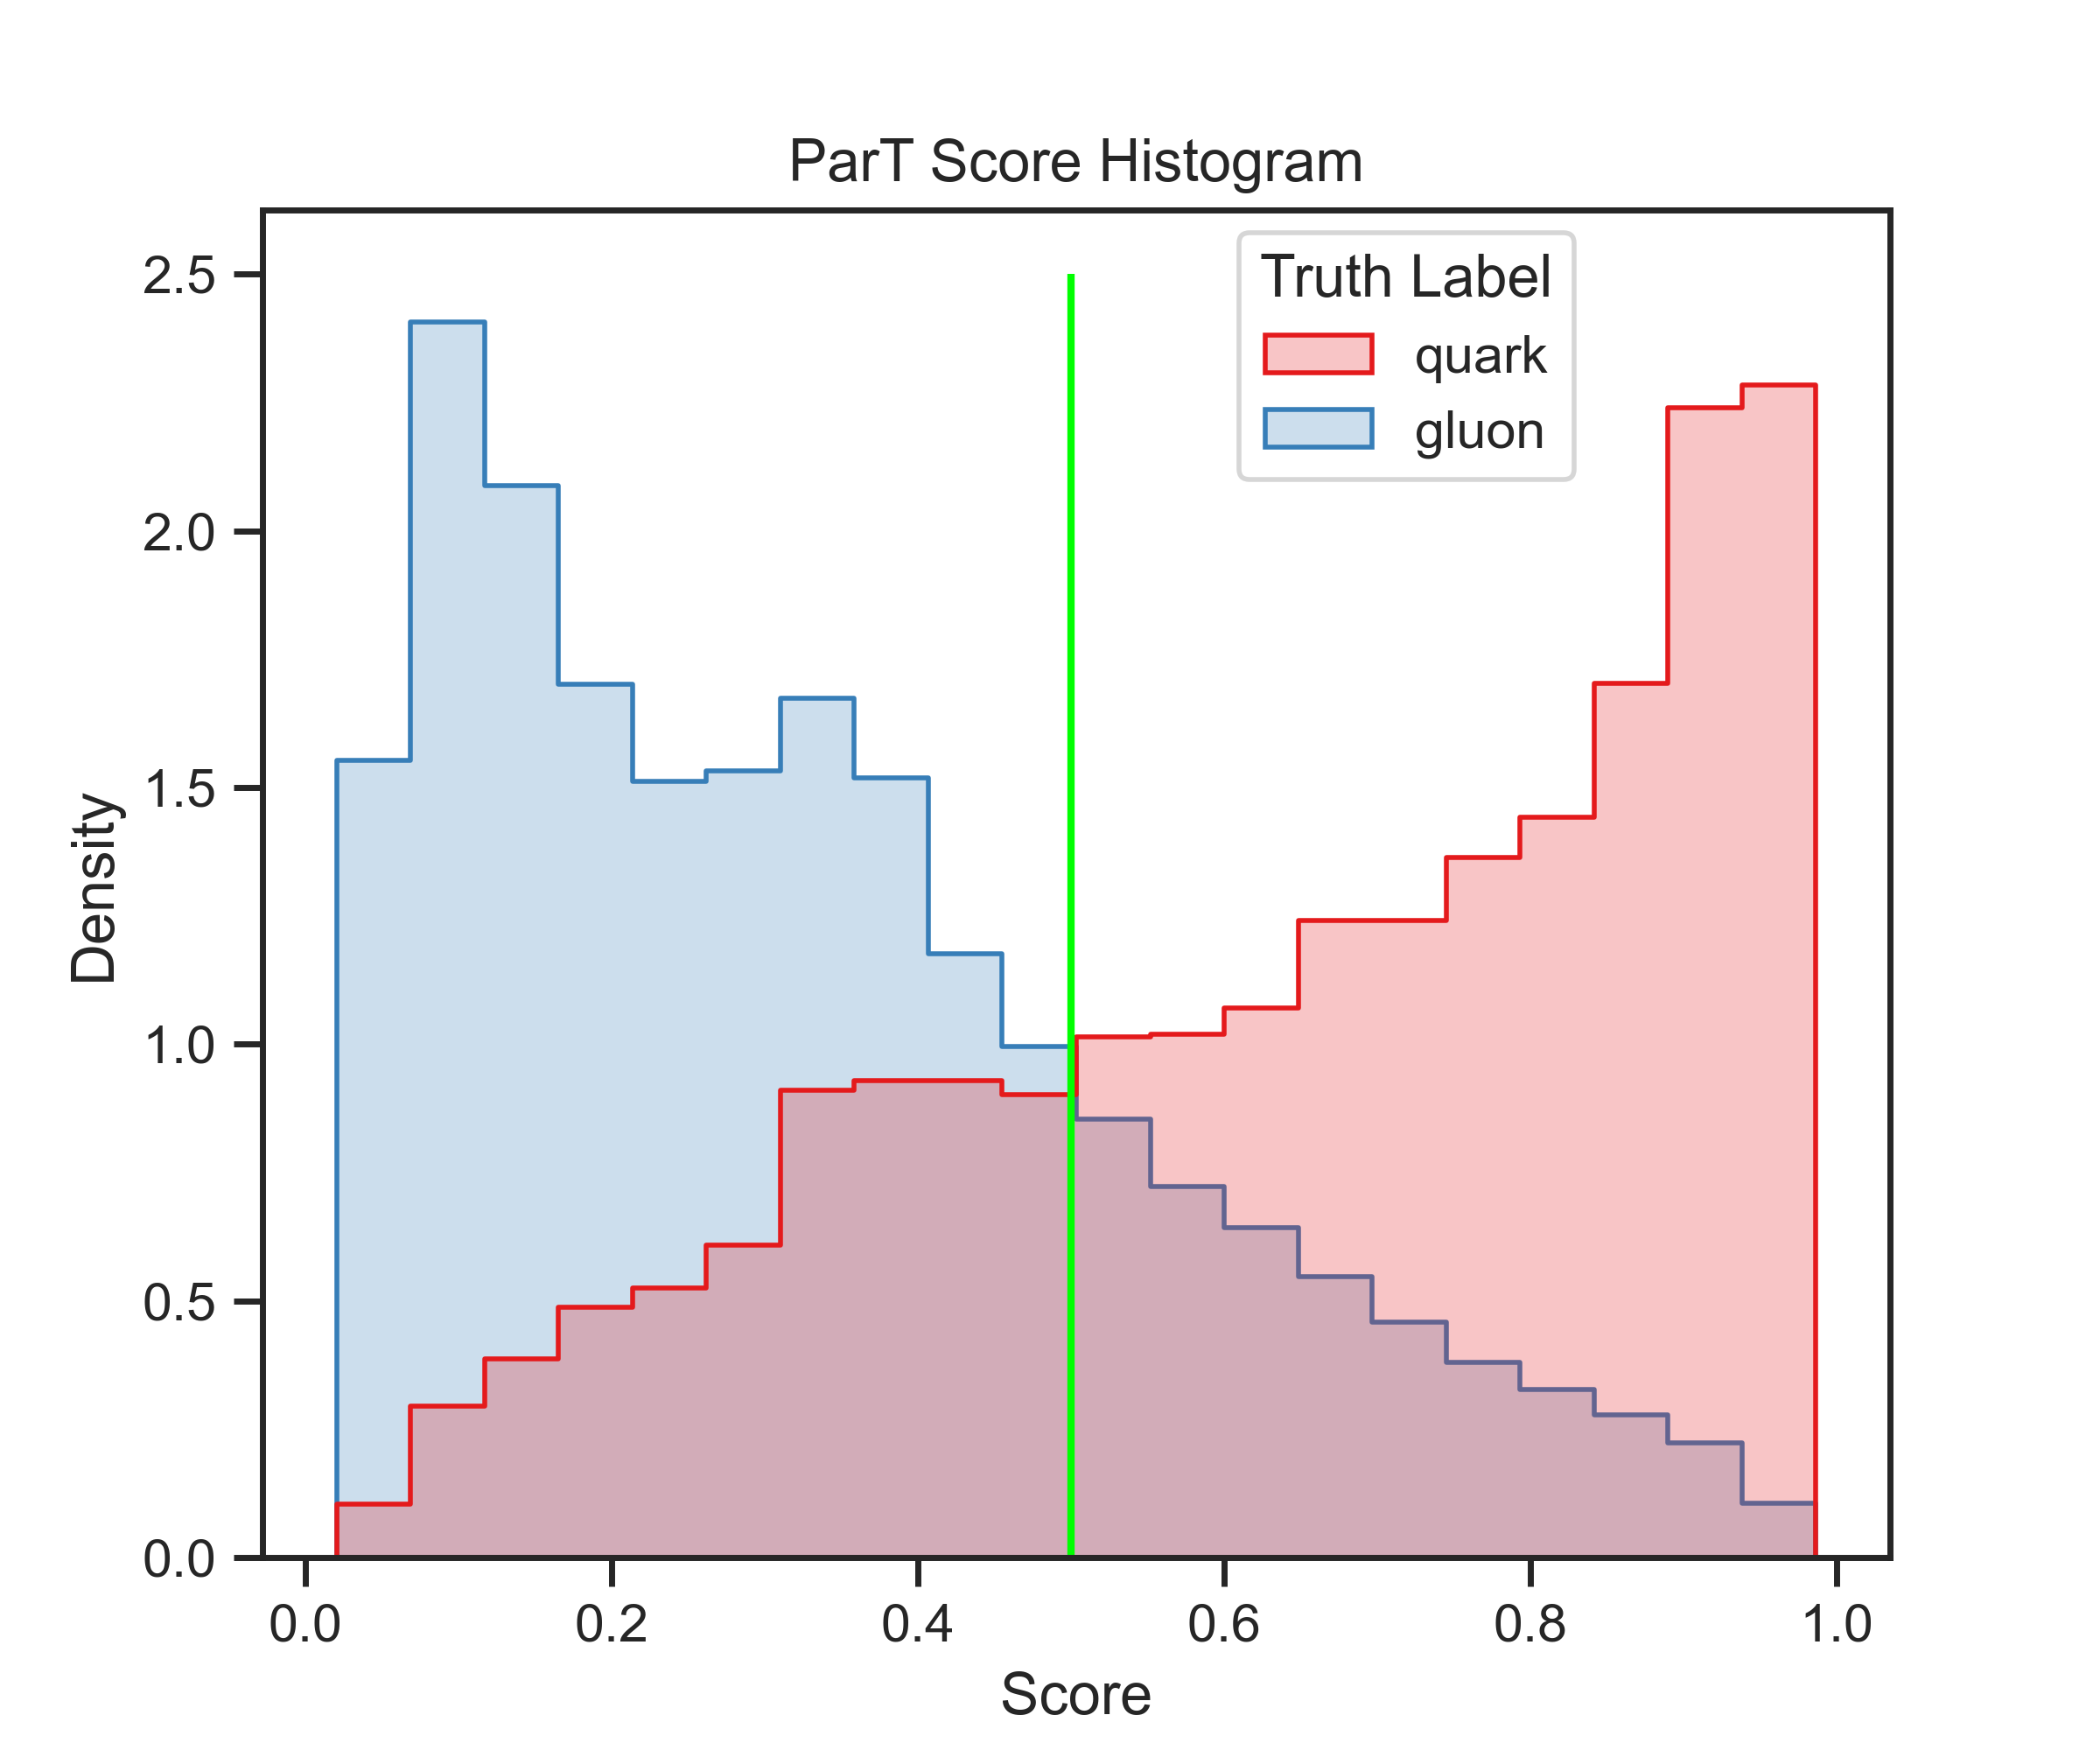
\includegraphics[width=1\textwidth]{src/plots/results/score/part.png}
		\caption{ParT}
		\label{fig:app_score_part}
	\end{subfigure}
	\begin{subfigure}[t]{0.49\textwidth}
		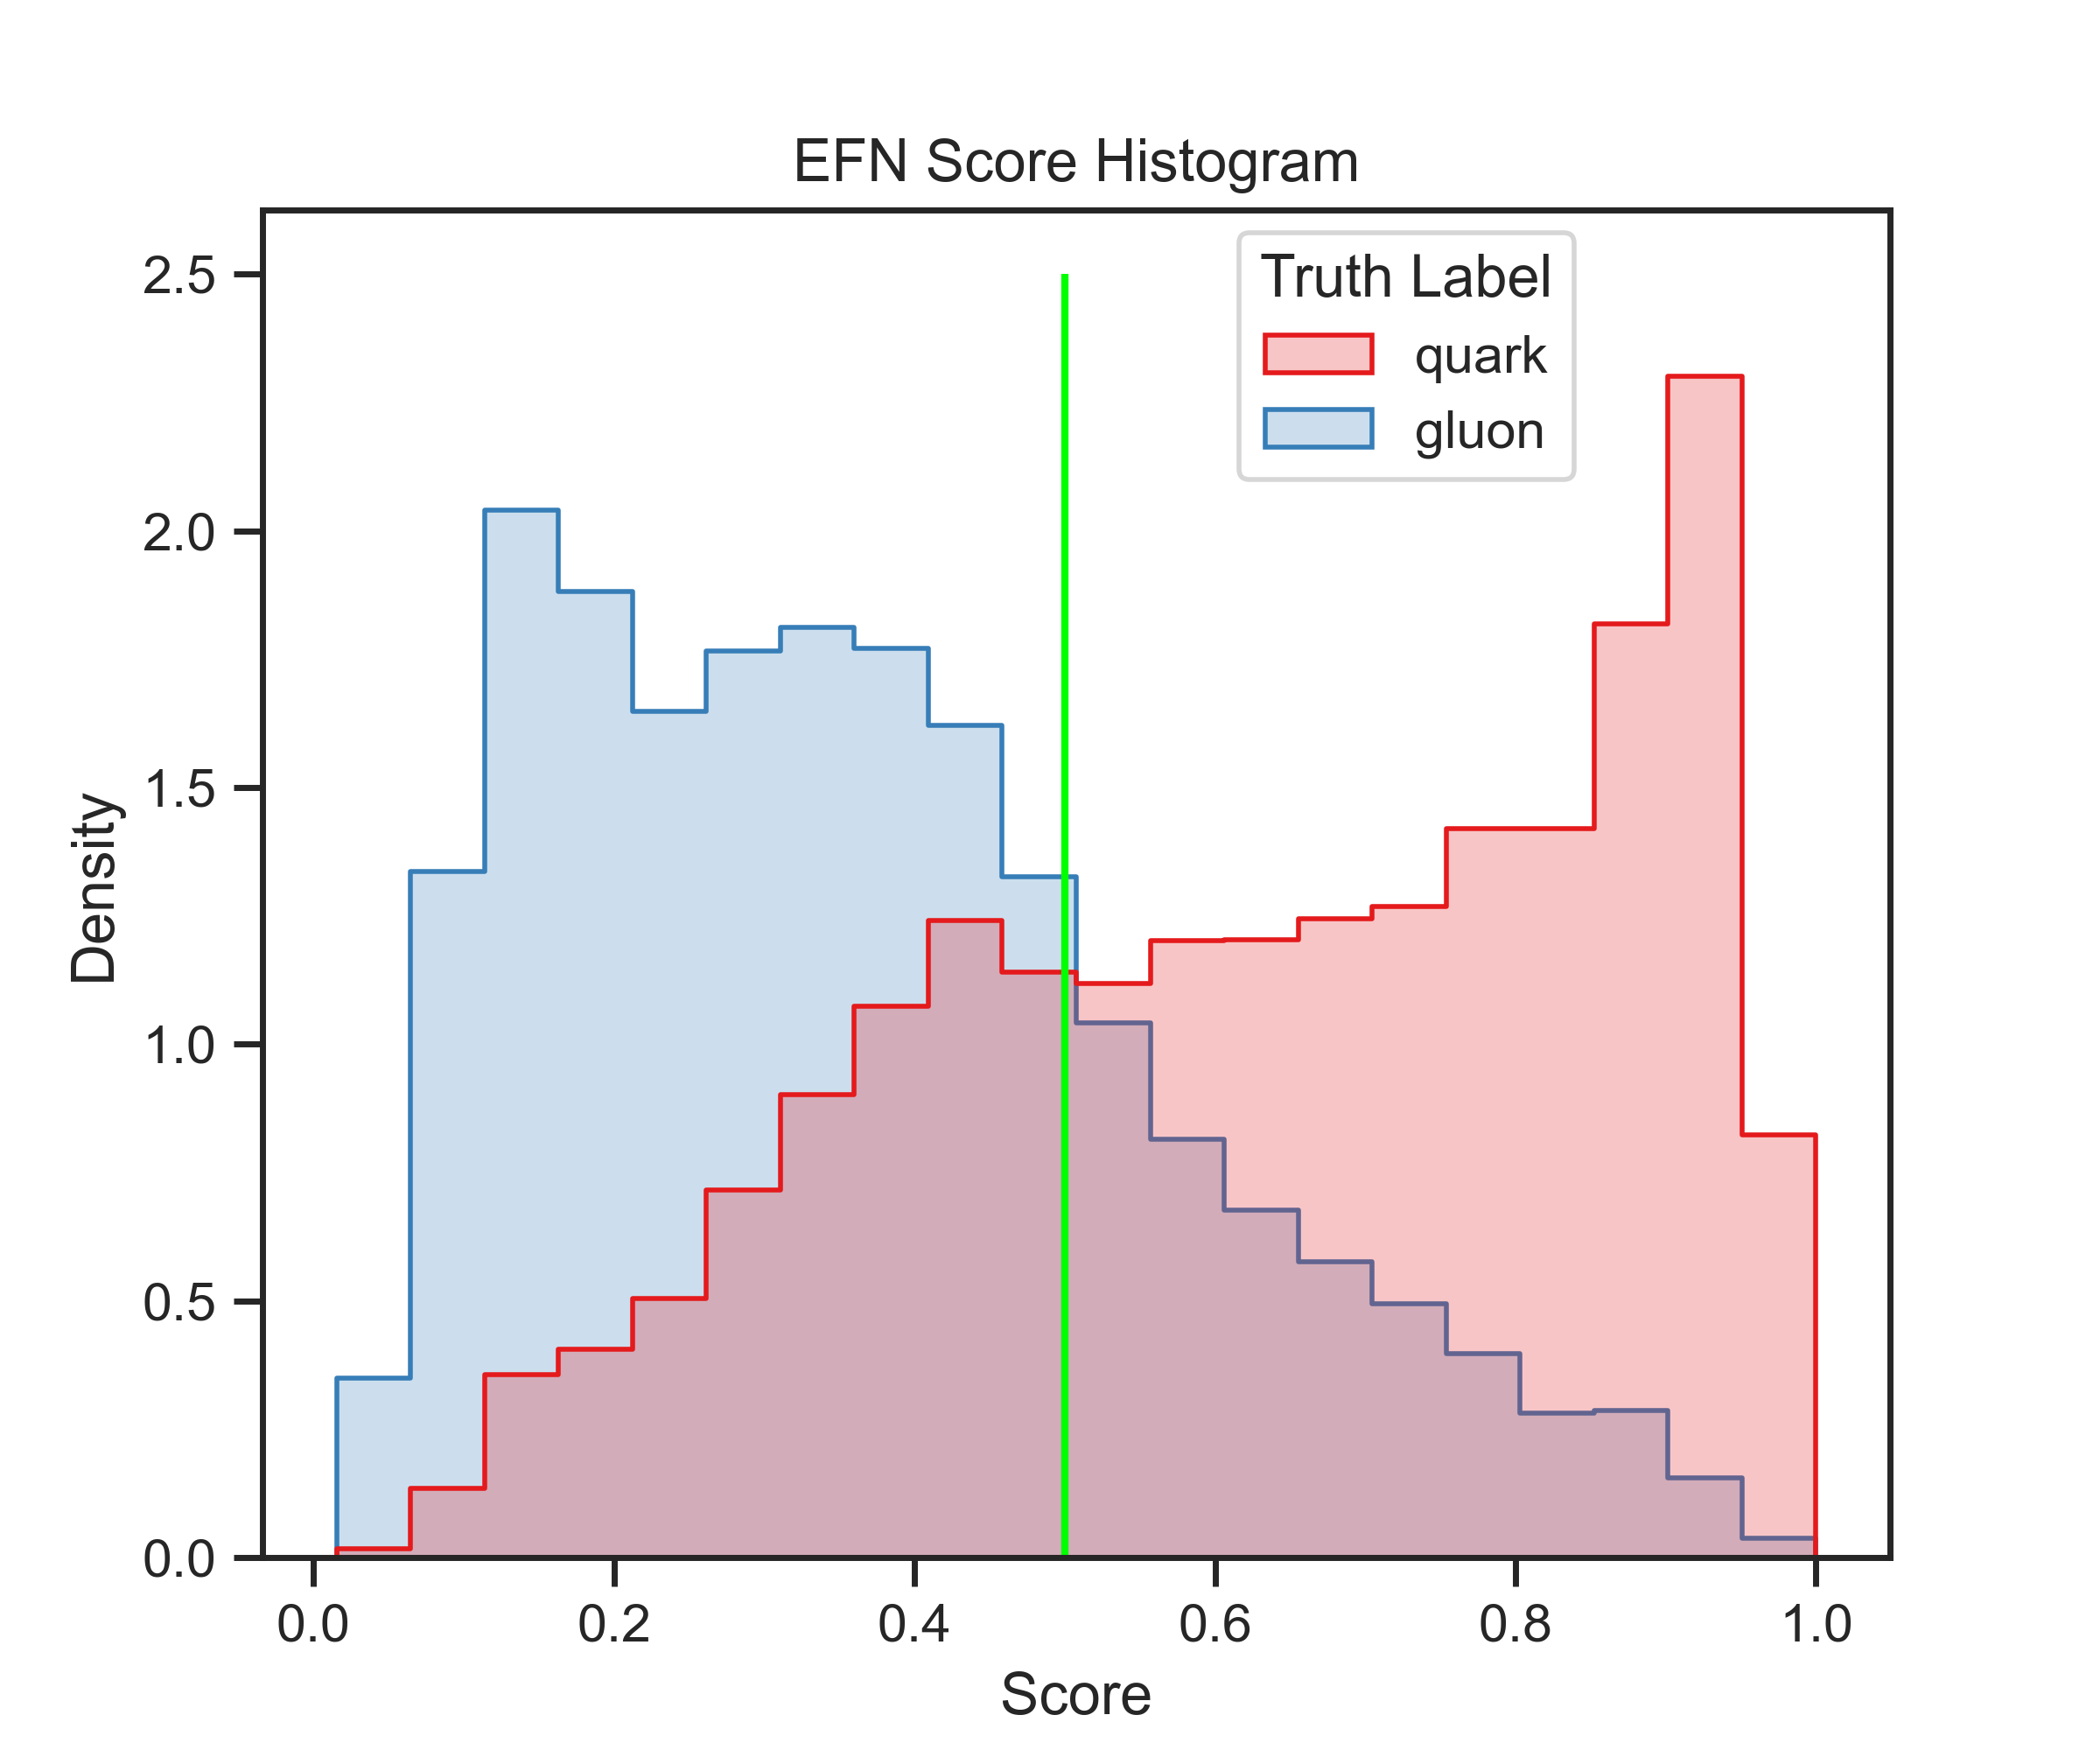
\includegraphics[width=1\textwidth]{src/plots/results/score/efn.png}
		\caption{EFN}
		\label{fig:app_score_efn}
	\end{subfigure}
\caption{Confusion Matricies}
\label{fig:app_score_5-9}
\end{figure}



\FloatBarrier

\section{Transverse Momentum Dependence}
\label{sec:app_pt_dep}


\begin{figure}[htb]
    \centering
    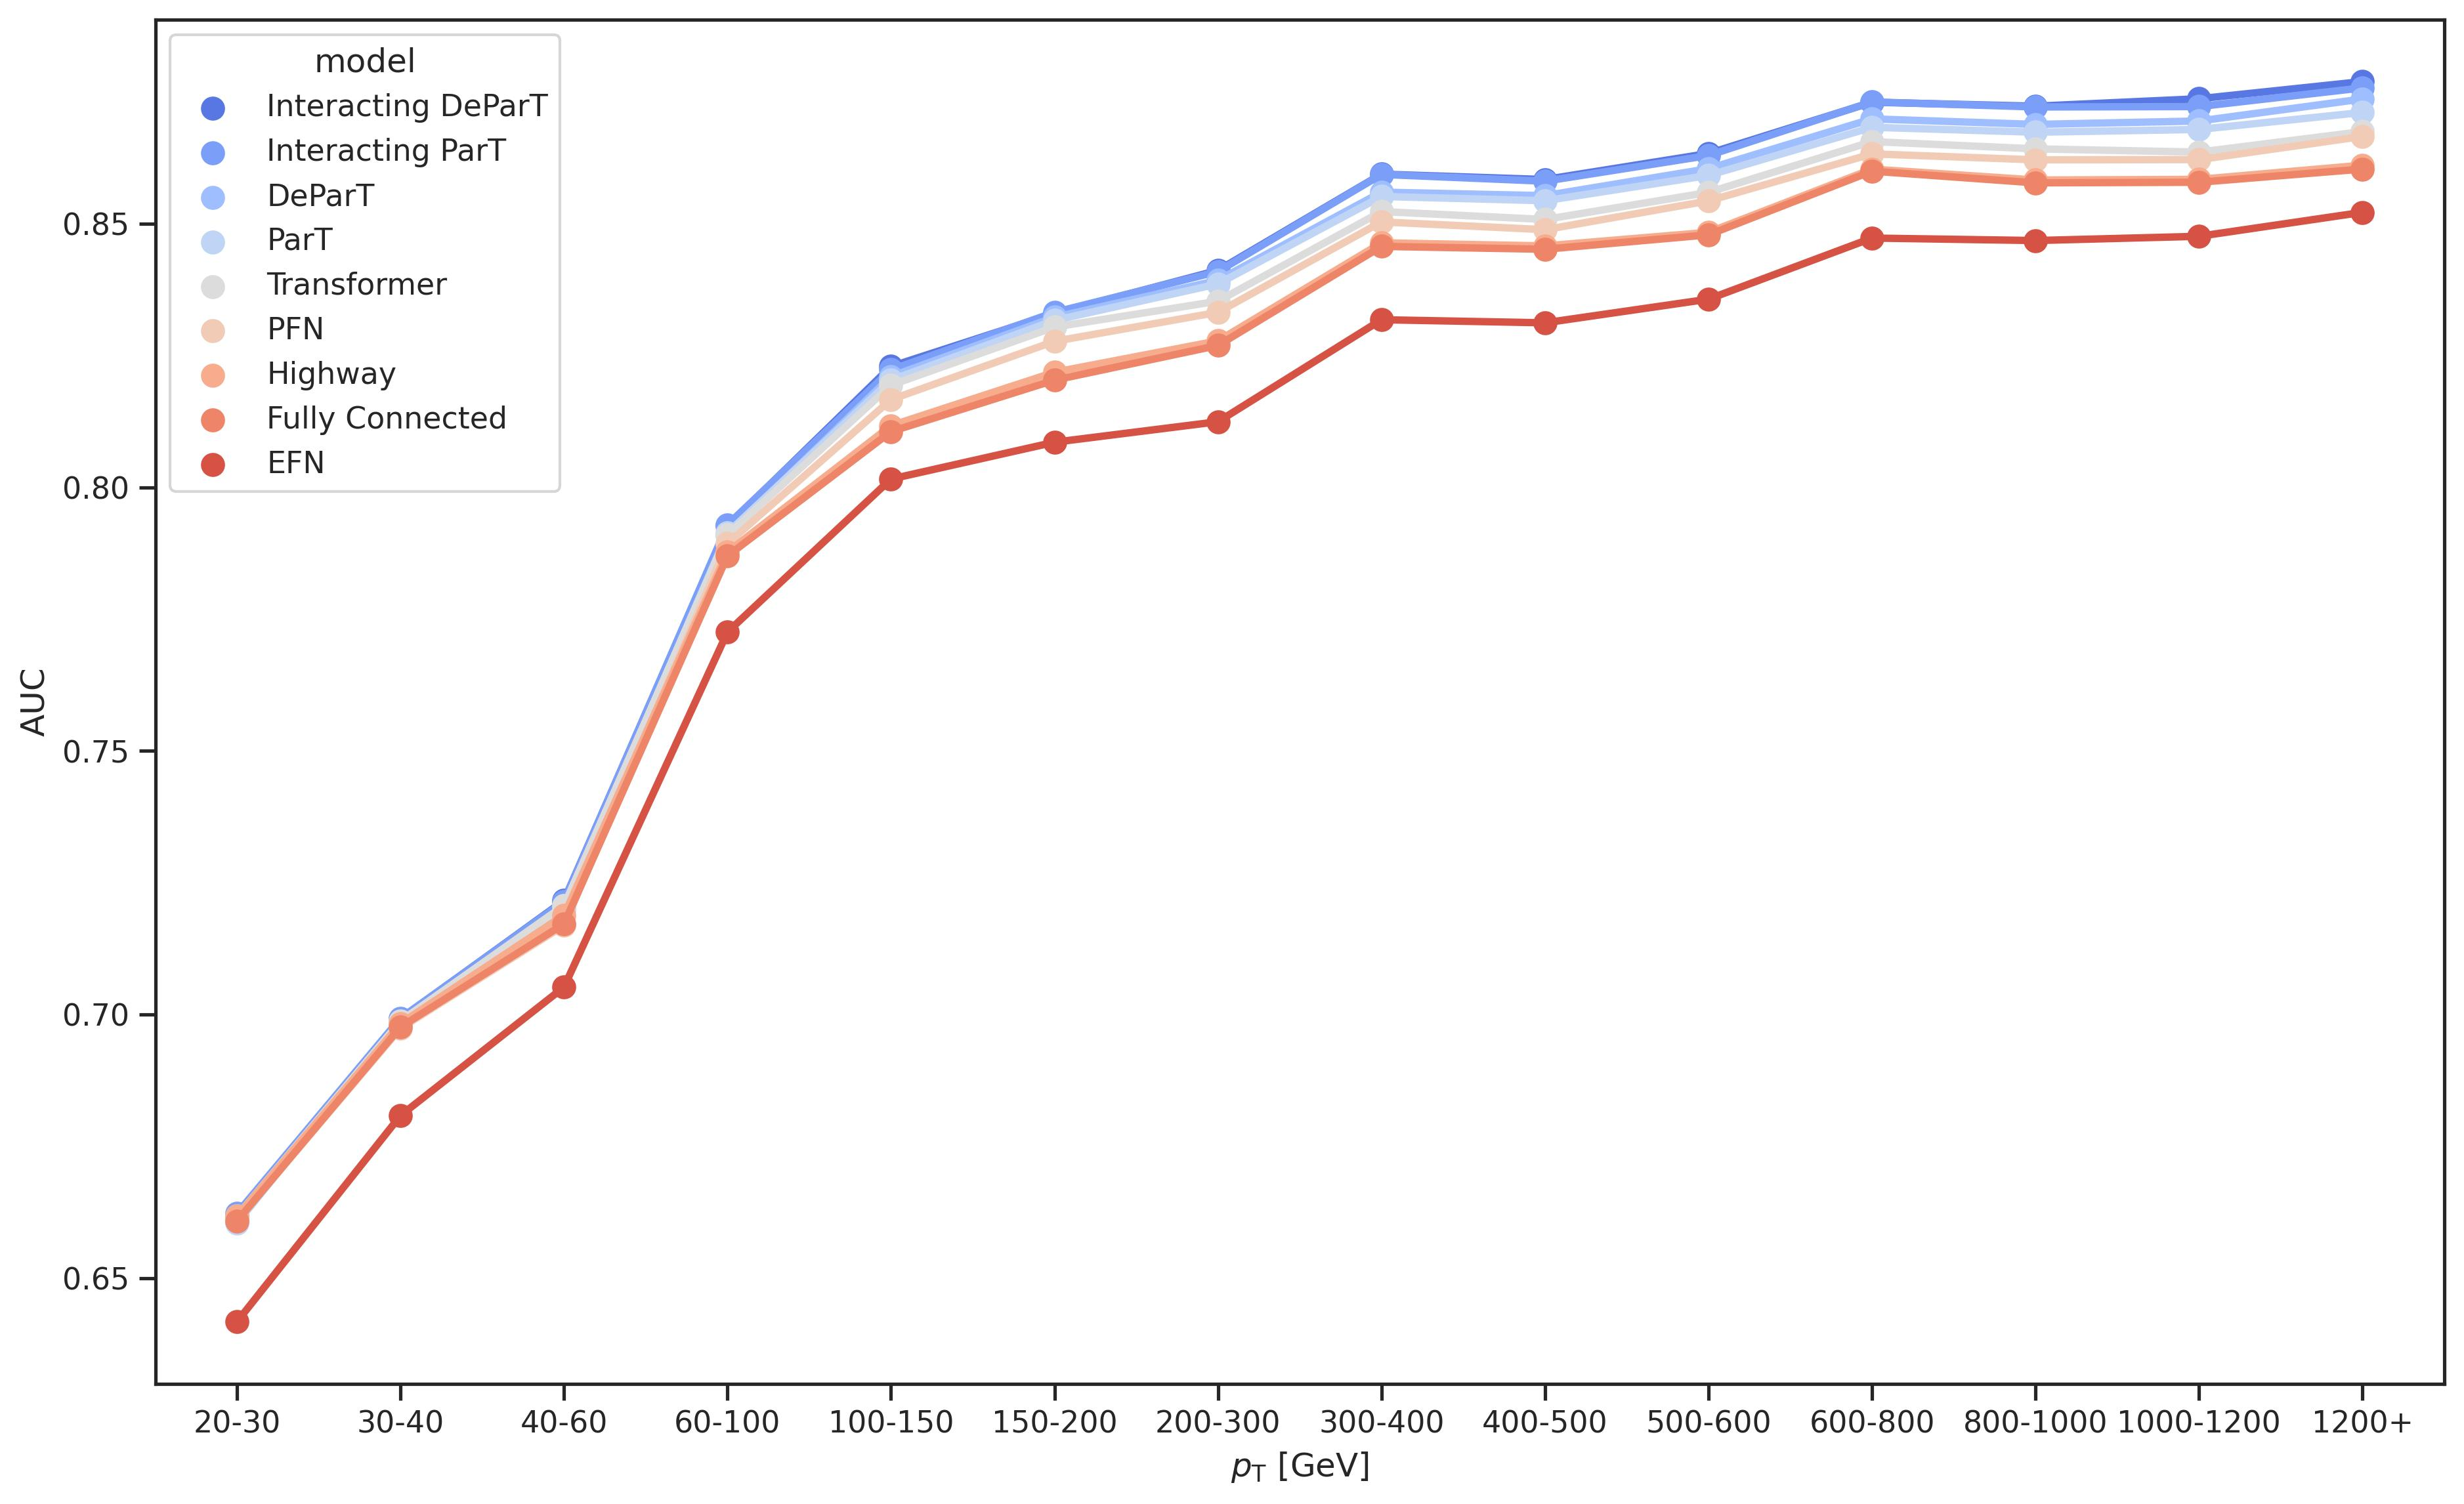
\includegraphics[width=0.95\linewidth]{src/plots/results/pT_dep/auc.jpg}
    \caption{AUC as a function of transverse momentum.}
    \label{fig:auc_pt}
\end{figure}

\begin{figure}[htb]
    \centering
    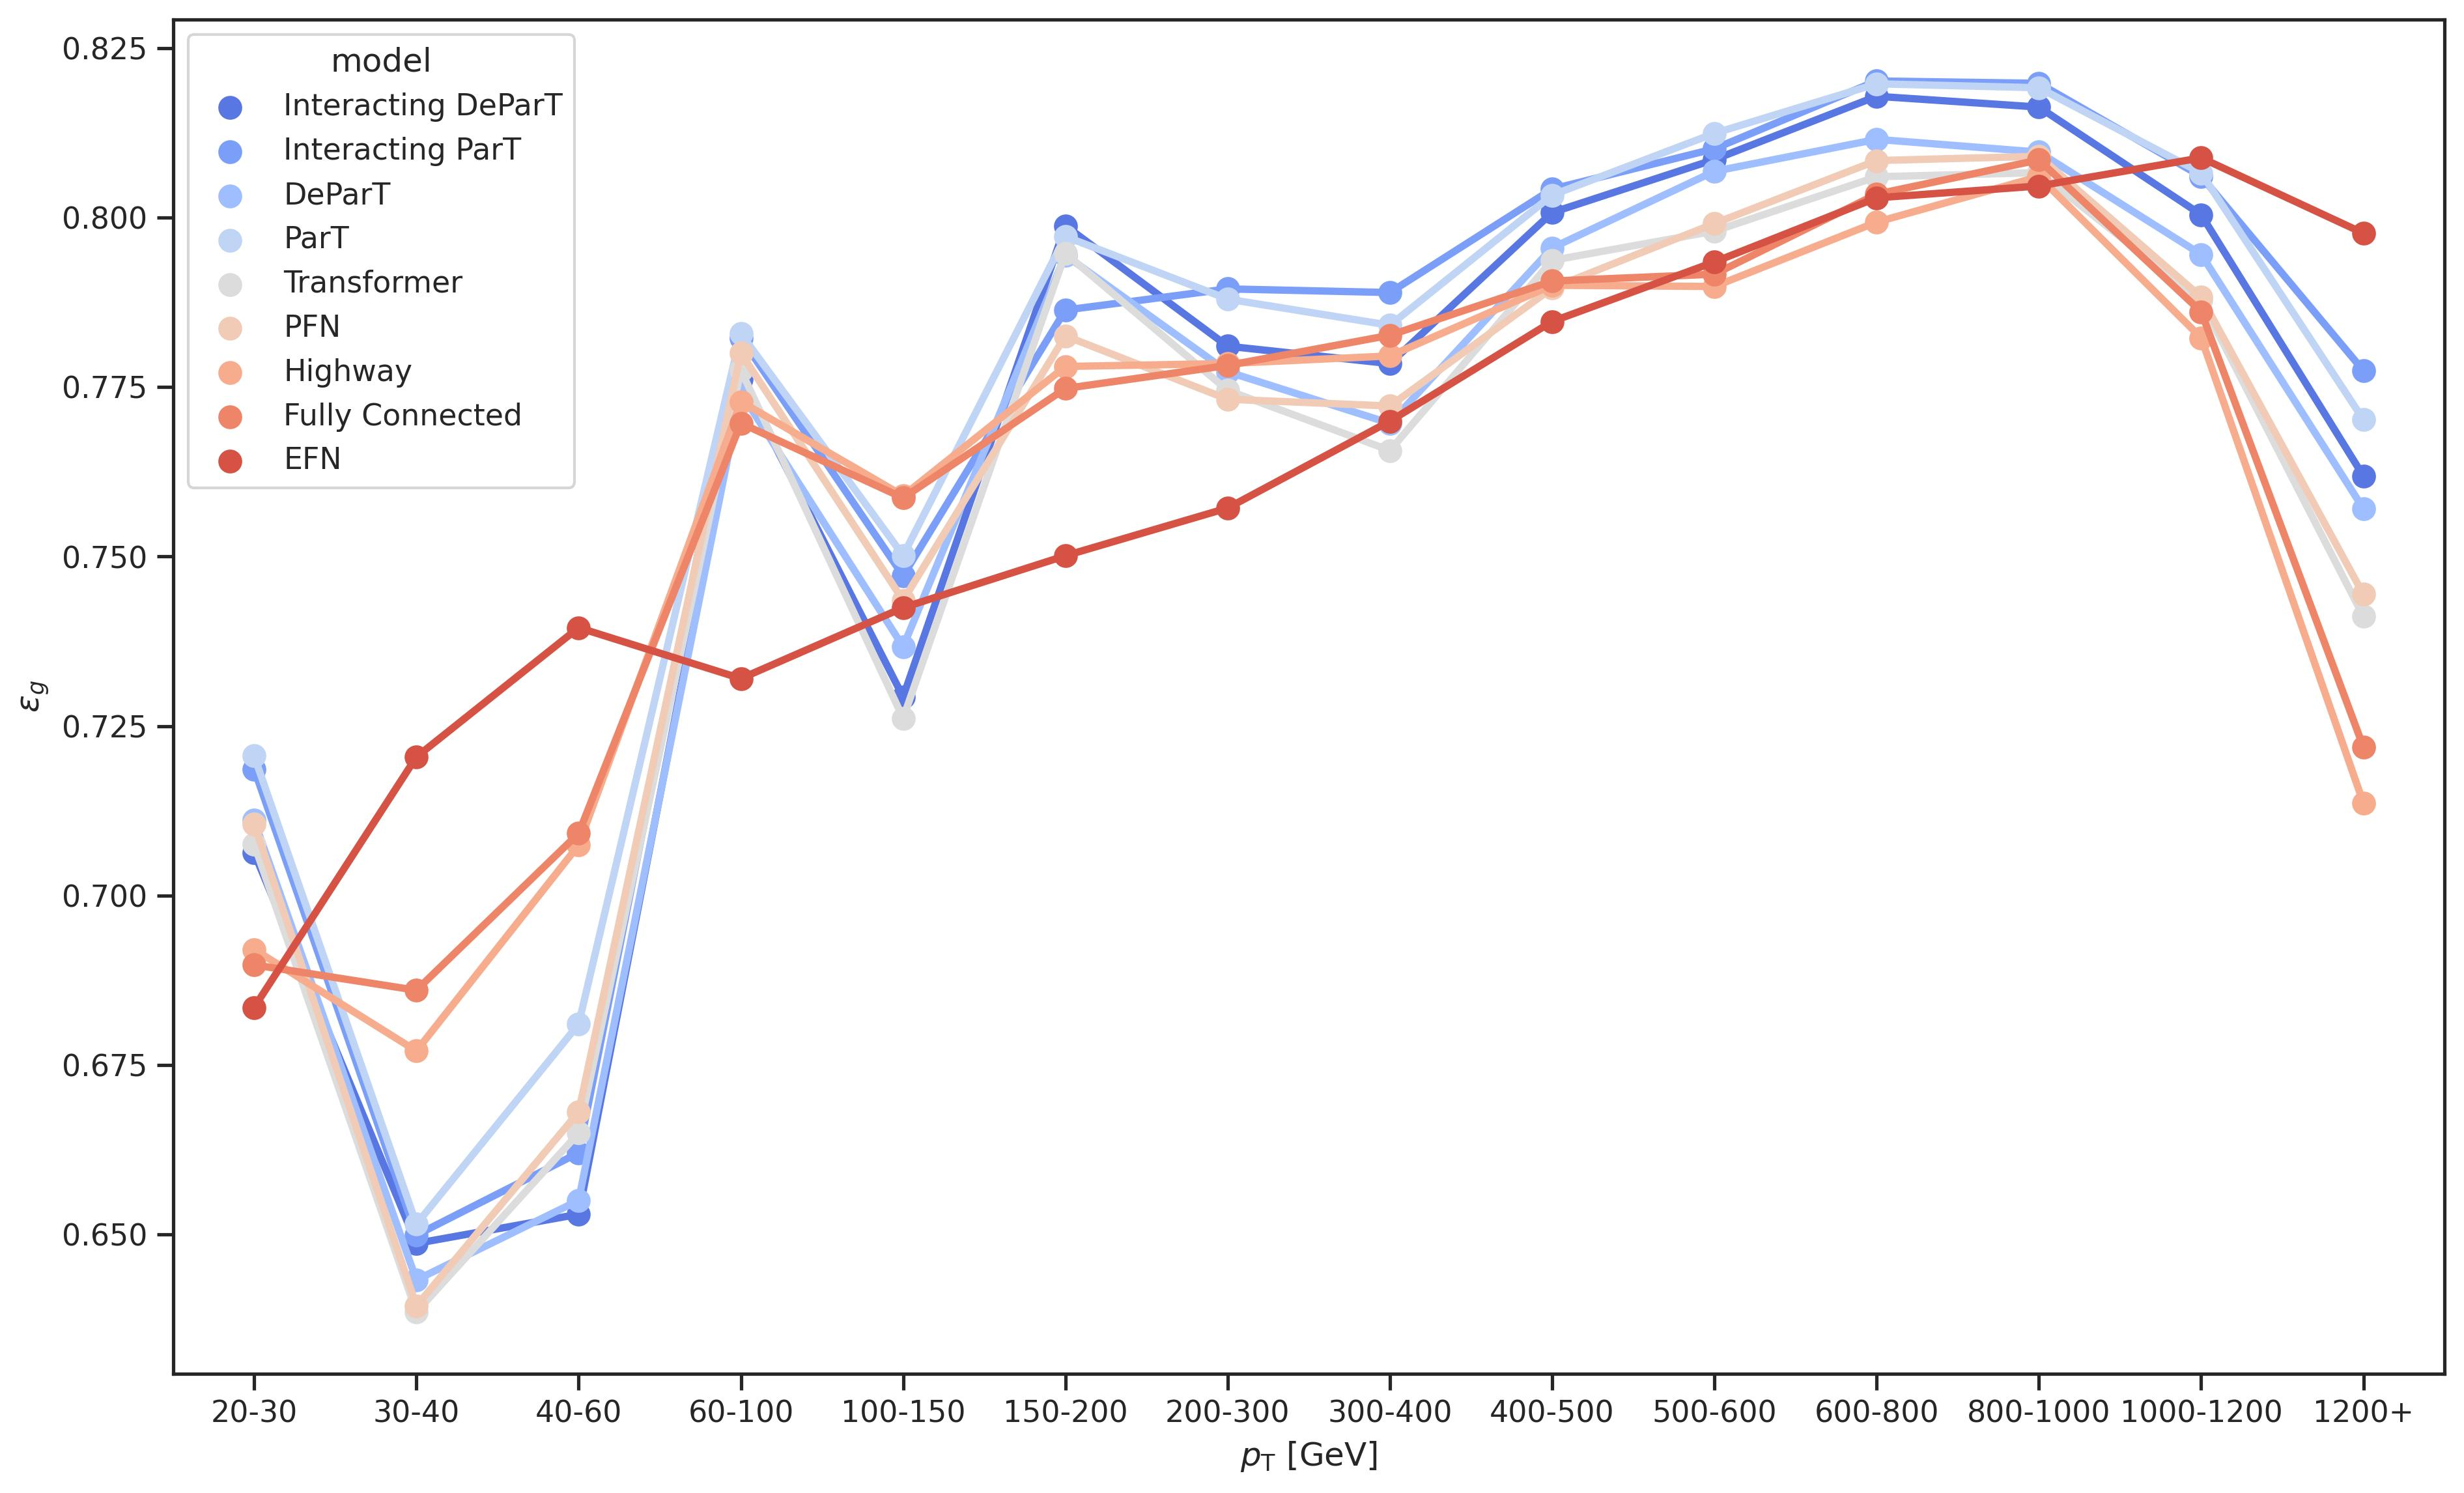
\includegraphics[width=0.95\linewidth]{src/plots/results/pT_dep/gluon_efficiency.jpg}
    \caption{Gluon efficiency as a function of transverse momentum.}
    \label{fig:gluon_eff_pt}
\end{figure}

\begin{figure}[htb]
    \centering
    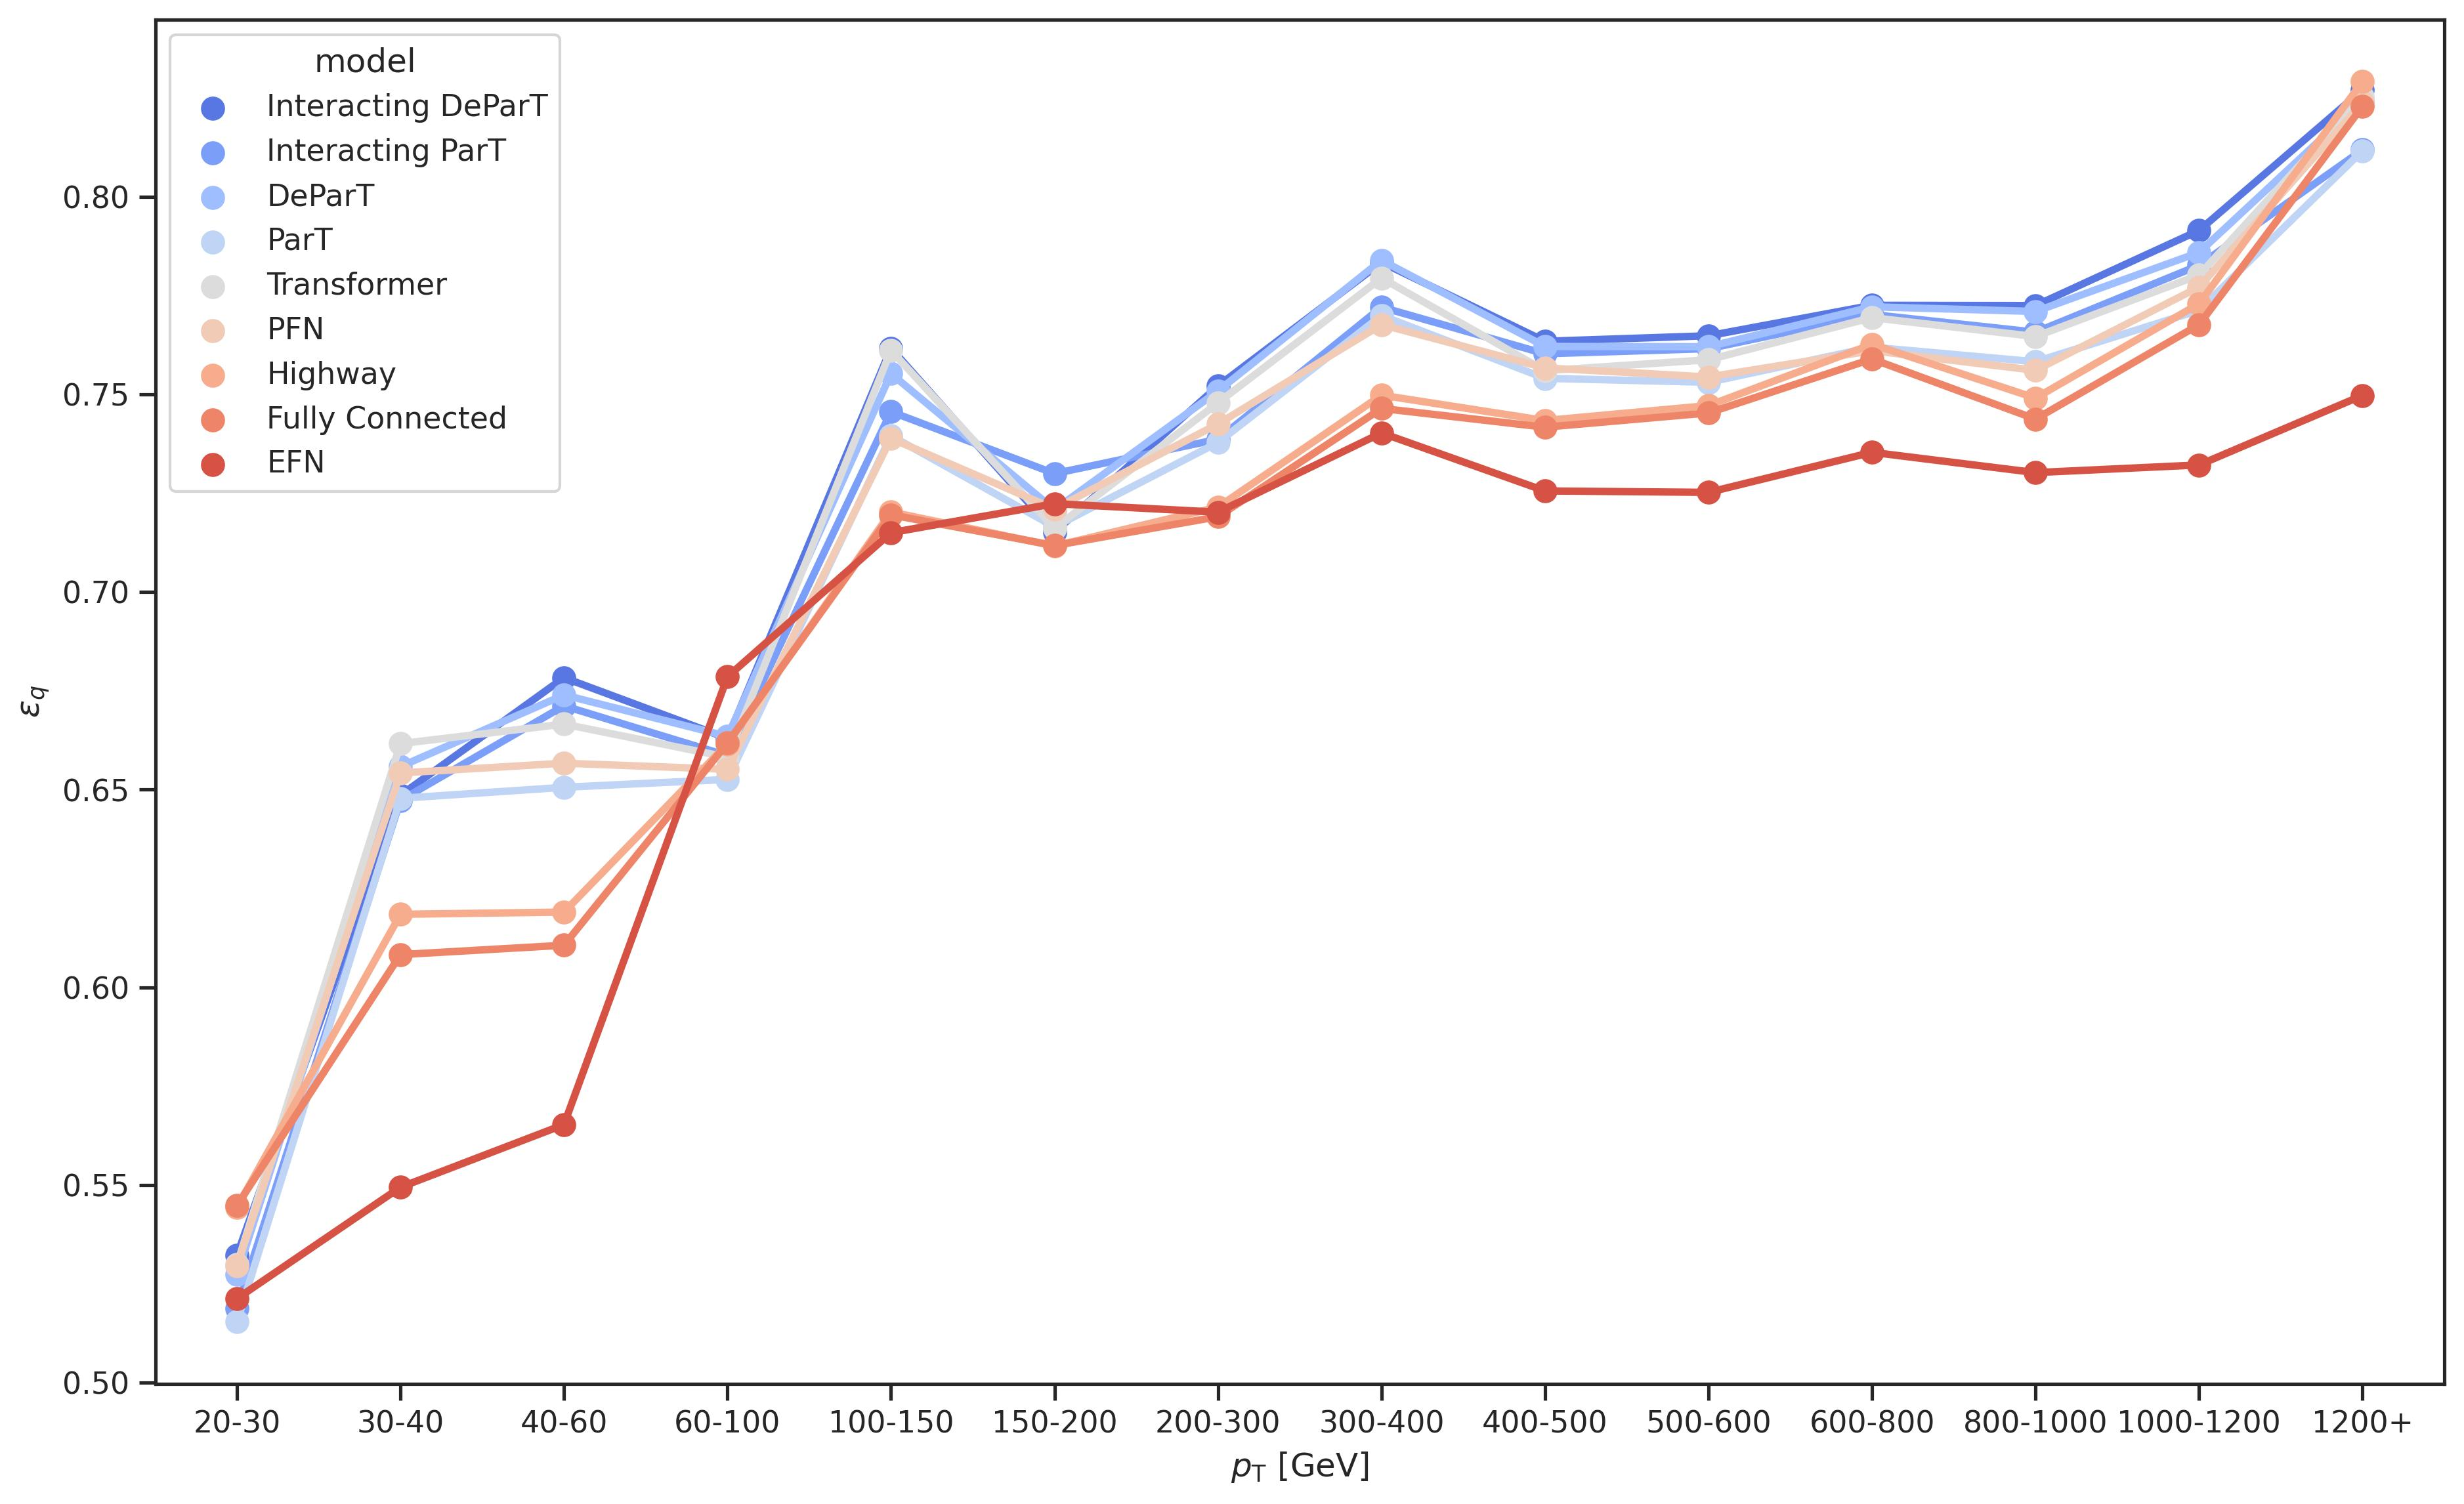
\includegraphics[width=0.95\linewidth]{src/plots/results/pT_dep/quark_efficiency.jpg}
    \caption{Quark efficiency as a function of transverse momentum.}
    \label{fig:quark_eff_pt}
\end{figure}

\begin{figure}[htb]
    \centering
    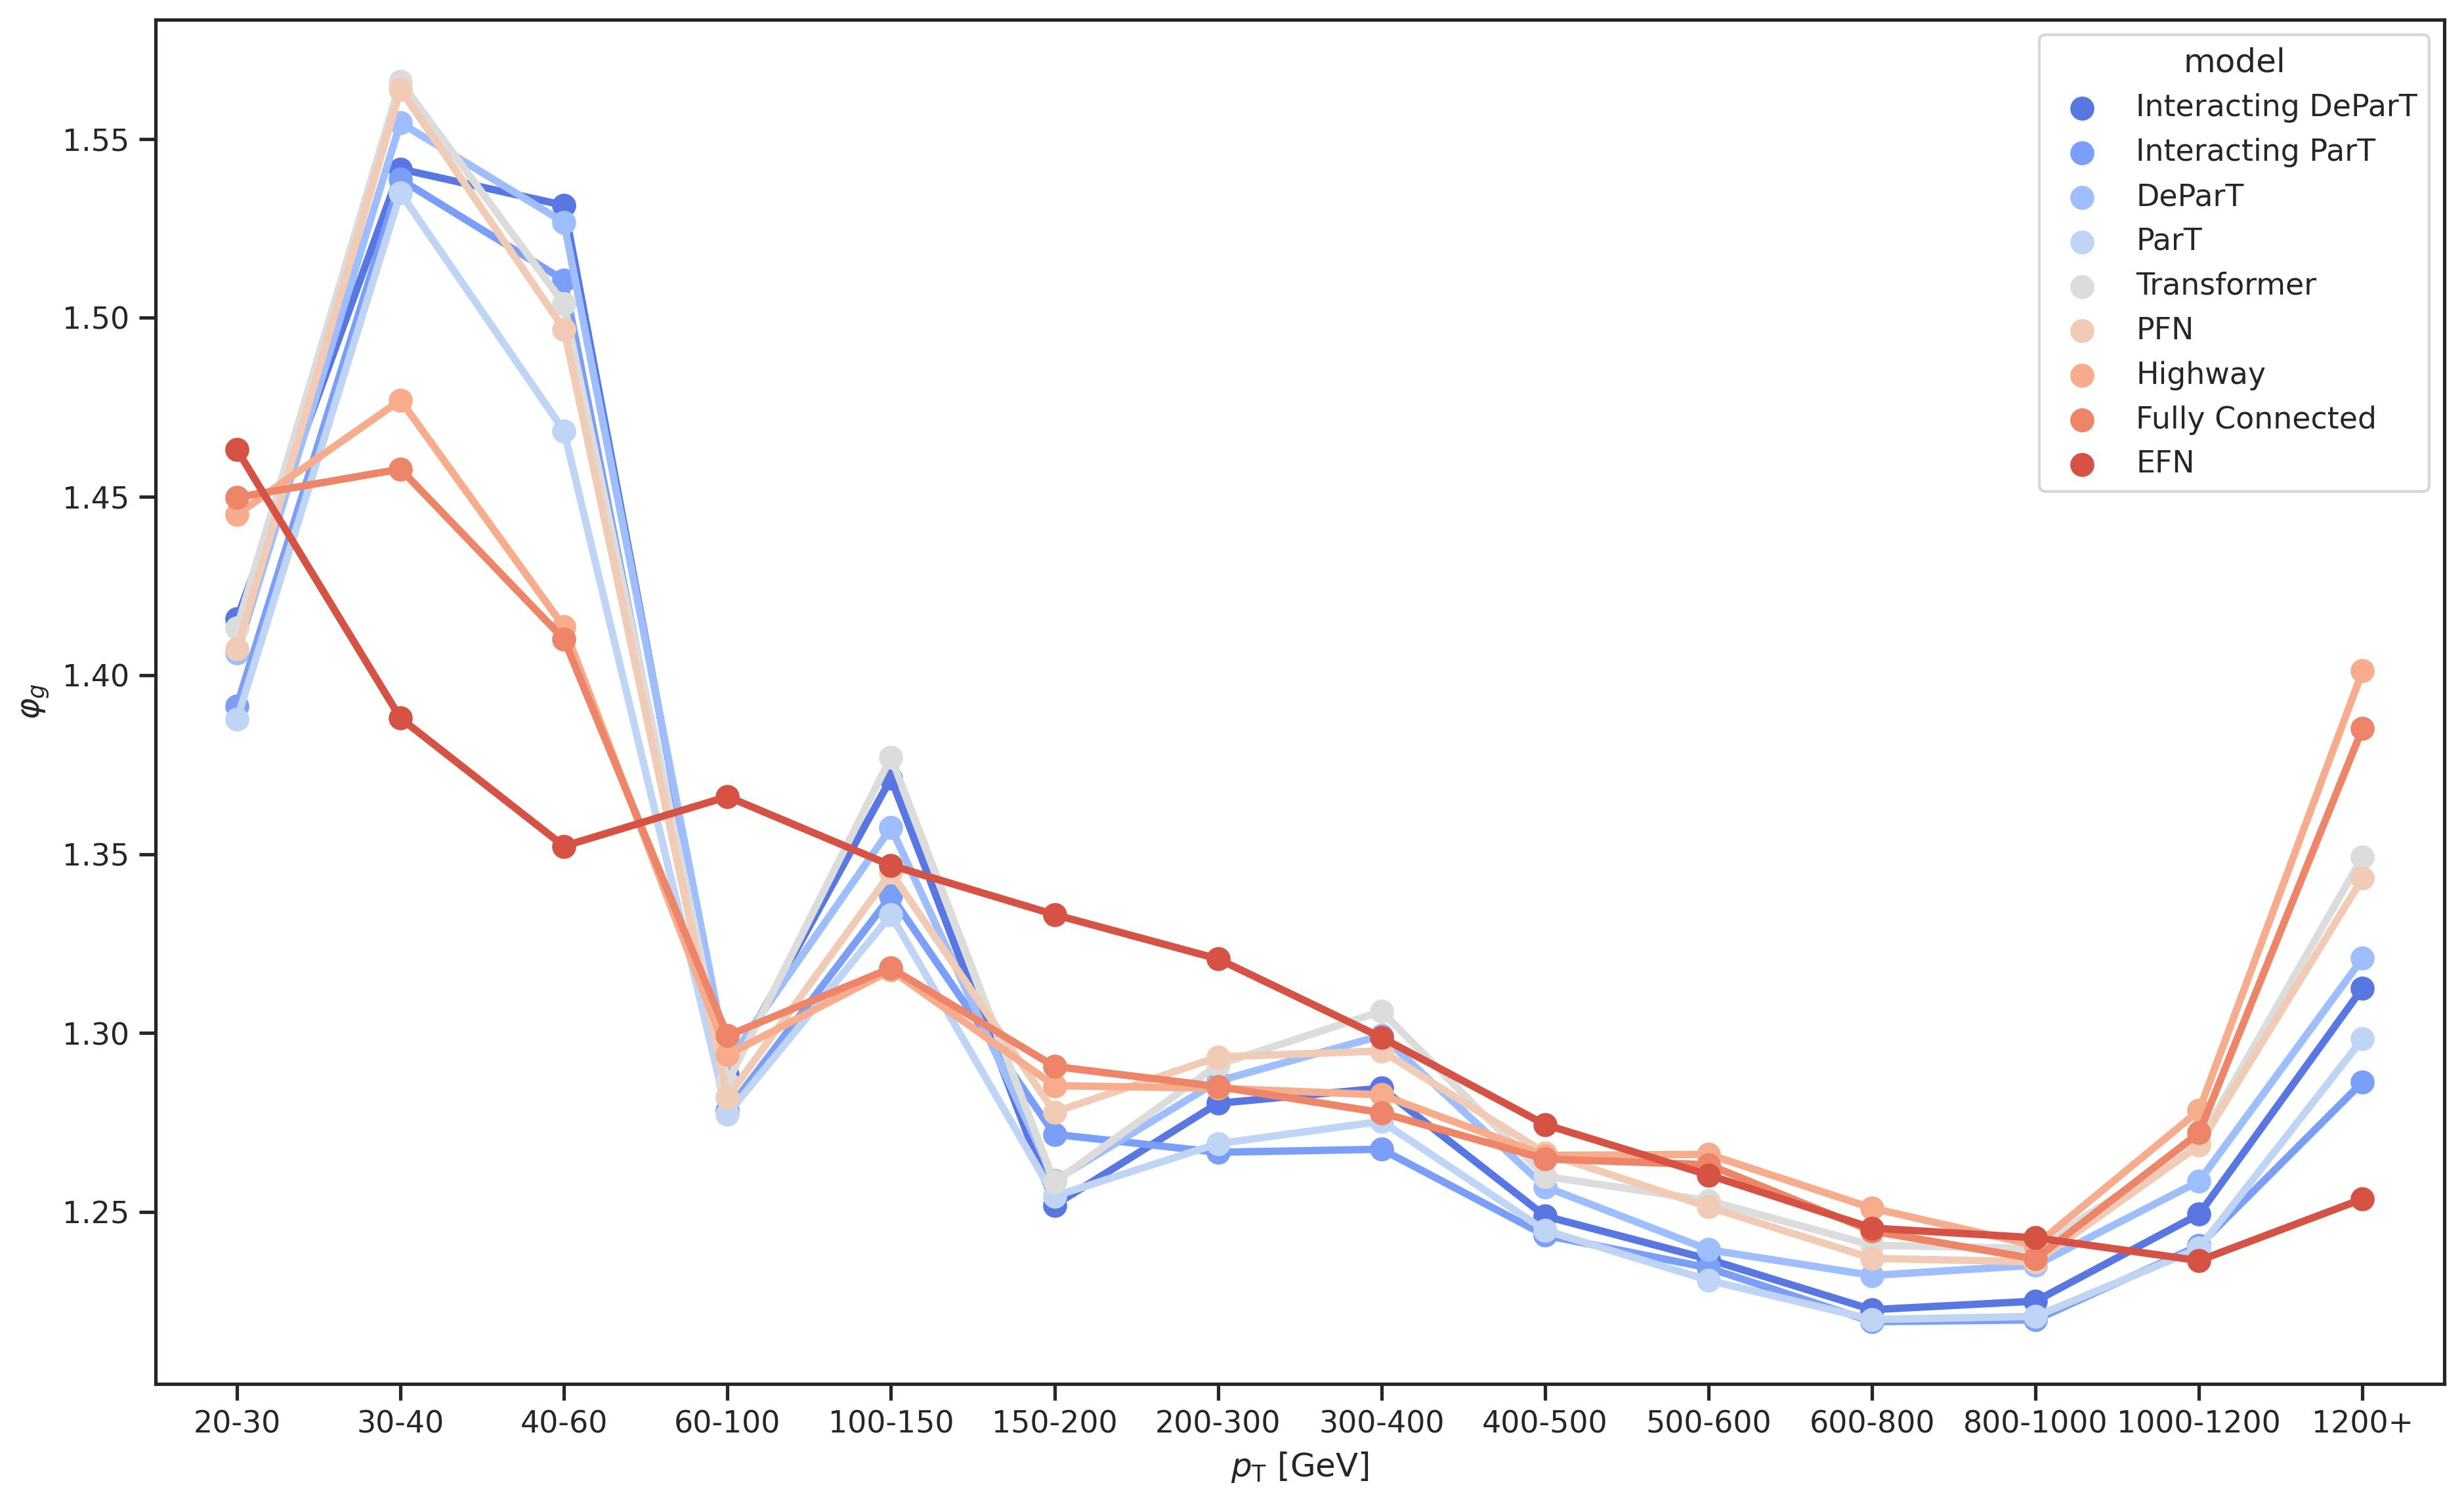
\includegraphics[width=0.95\linewidth]{src/plots/results/pT_dep/gluon_rejection.jpg}
    \caption{Gluon rejection as a function of transverse momentum.}
    \label{fig:gluon_rej_pt}
\end{figure}

\begin{figure}[htb]
    \centering
    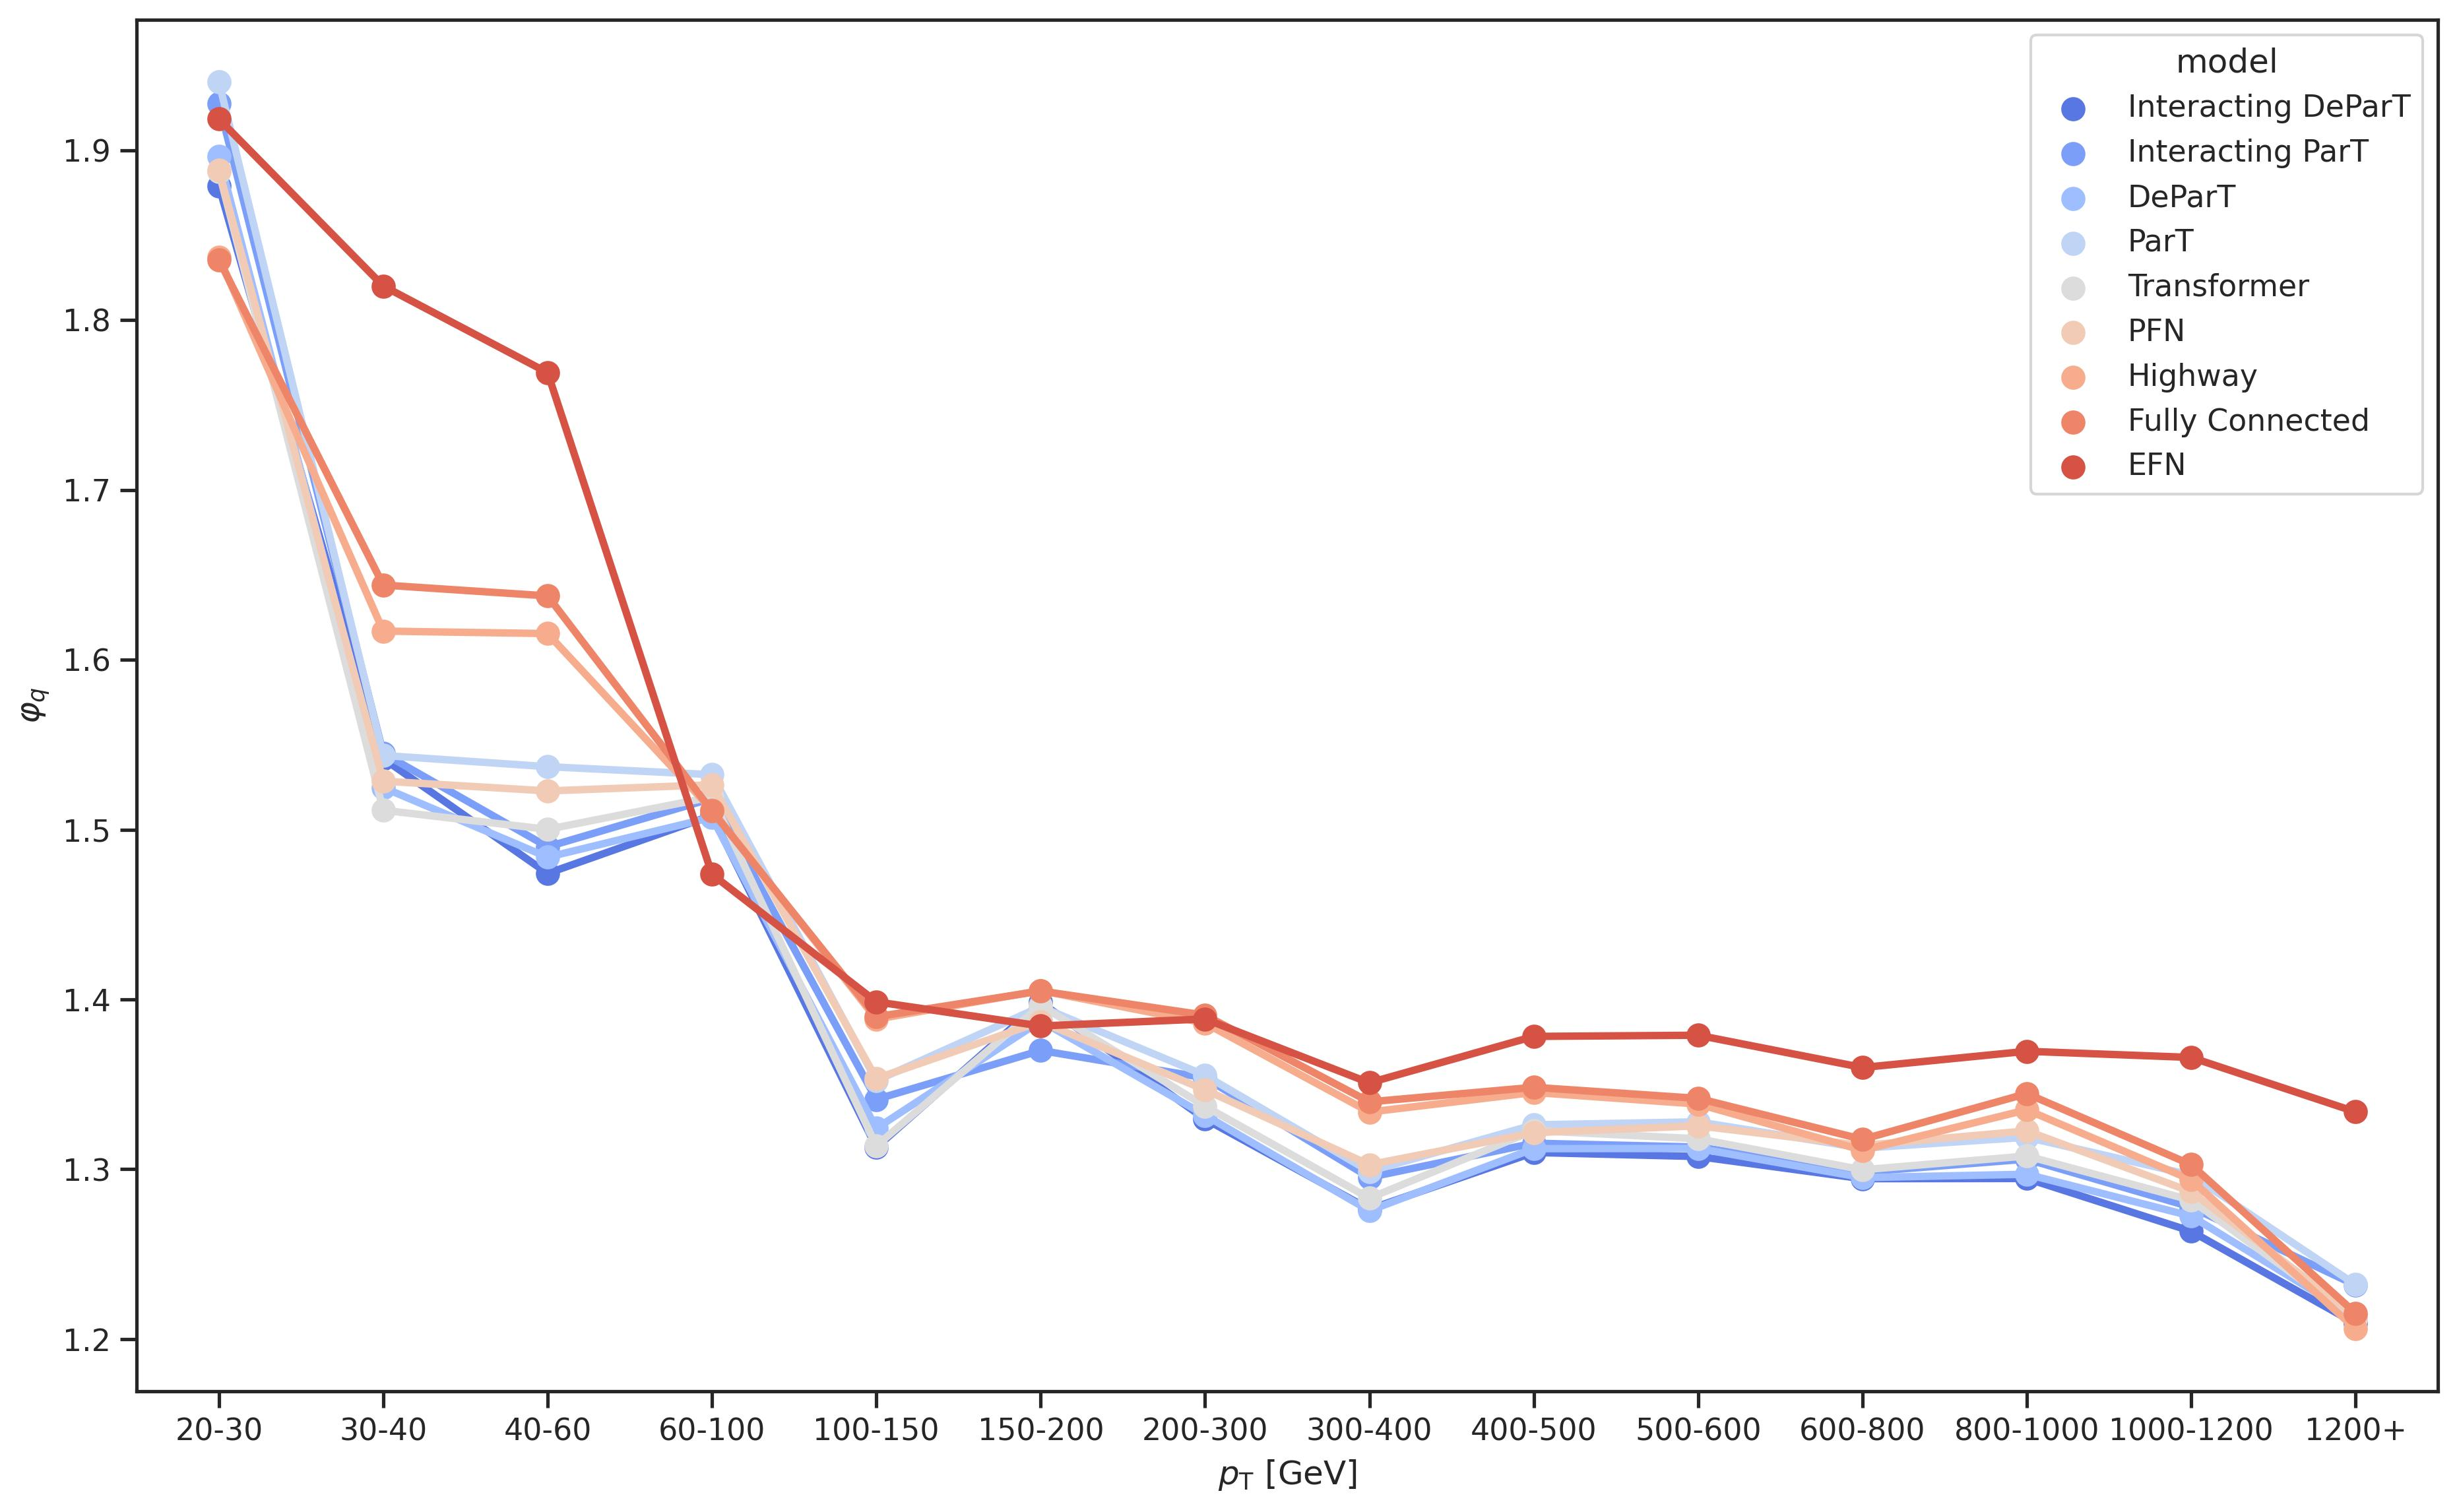
\includegraphics[width=0.95\linewidth]{src/plots/results/pT_dep/quark_rejection.jpg}
    \caption{Quark rejection as a function of transverse momentum.}
    \label{fig:quark_rej_pt}
\end{figure}

\begin{figure}[htb]
    \centering
    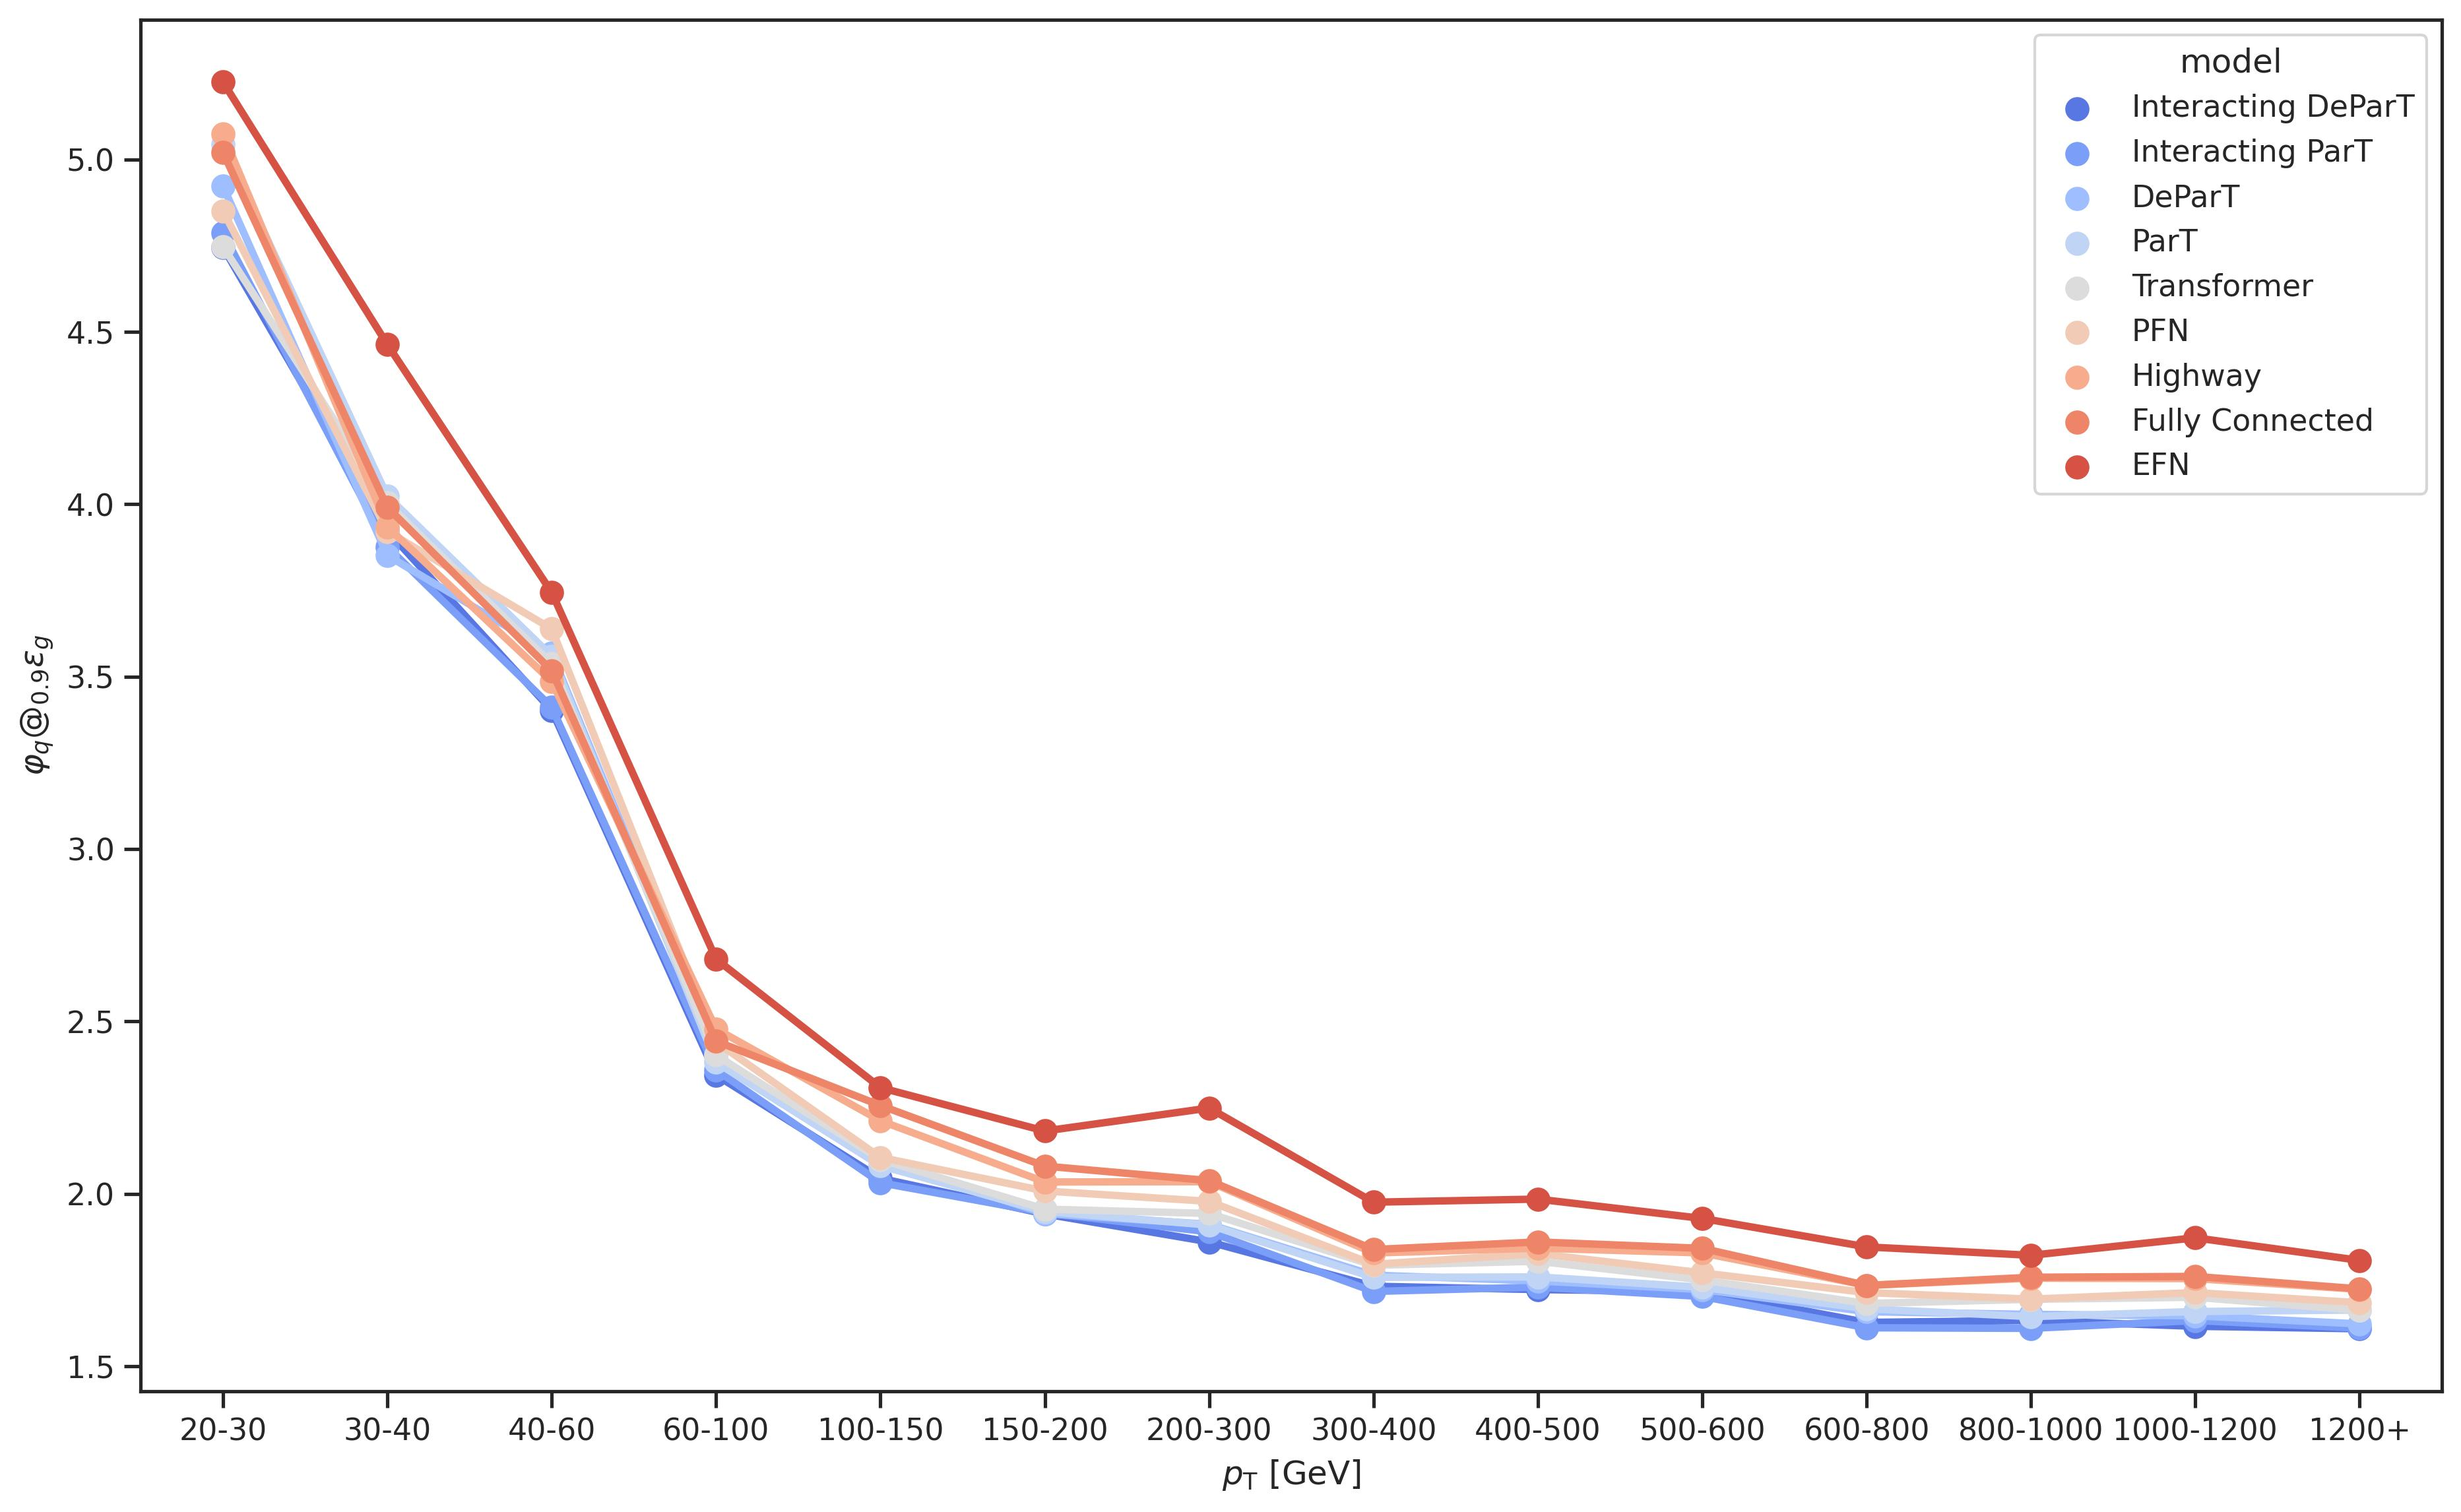
\includegraphics[width=0.95\linewidth]{src/plots/results/pT_dep/quark_rej_at_gluon_eff_0.9.jpg}
    \caption{Quark rejection at gluon efficiency of 0.9 as a function of transverse momentum.}
    \label{fig:quark_rej_at_gluon_eff_0.9_pt}
\end{figure}

\begin{figure}[htb]
    \centering
    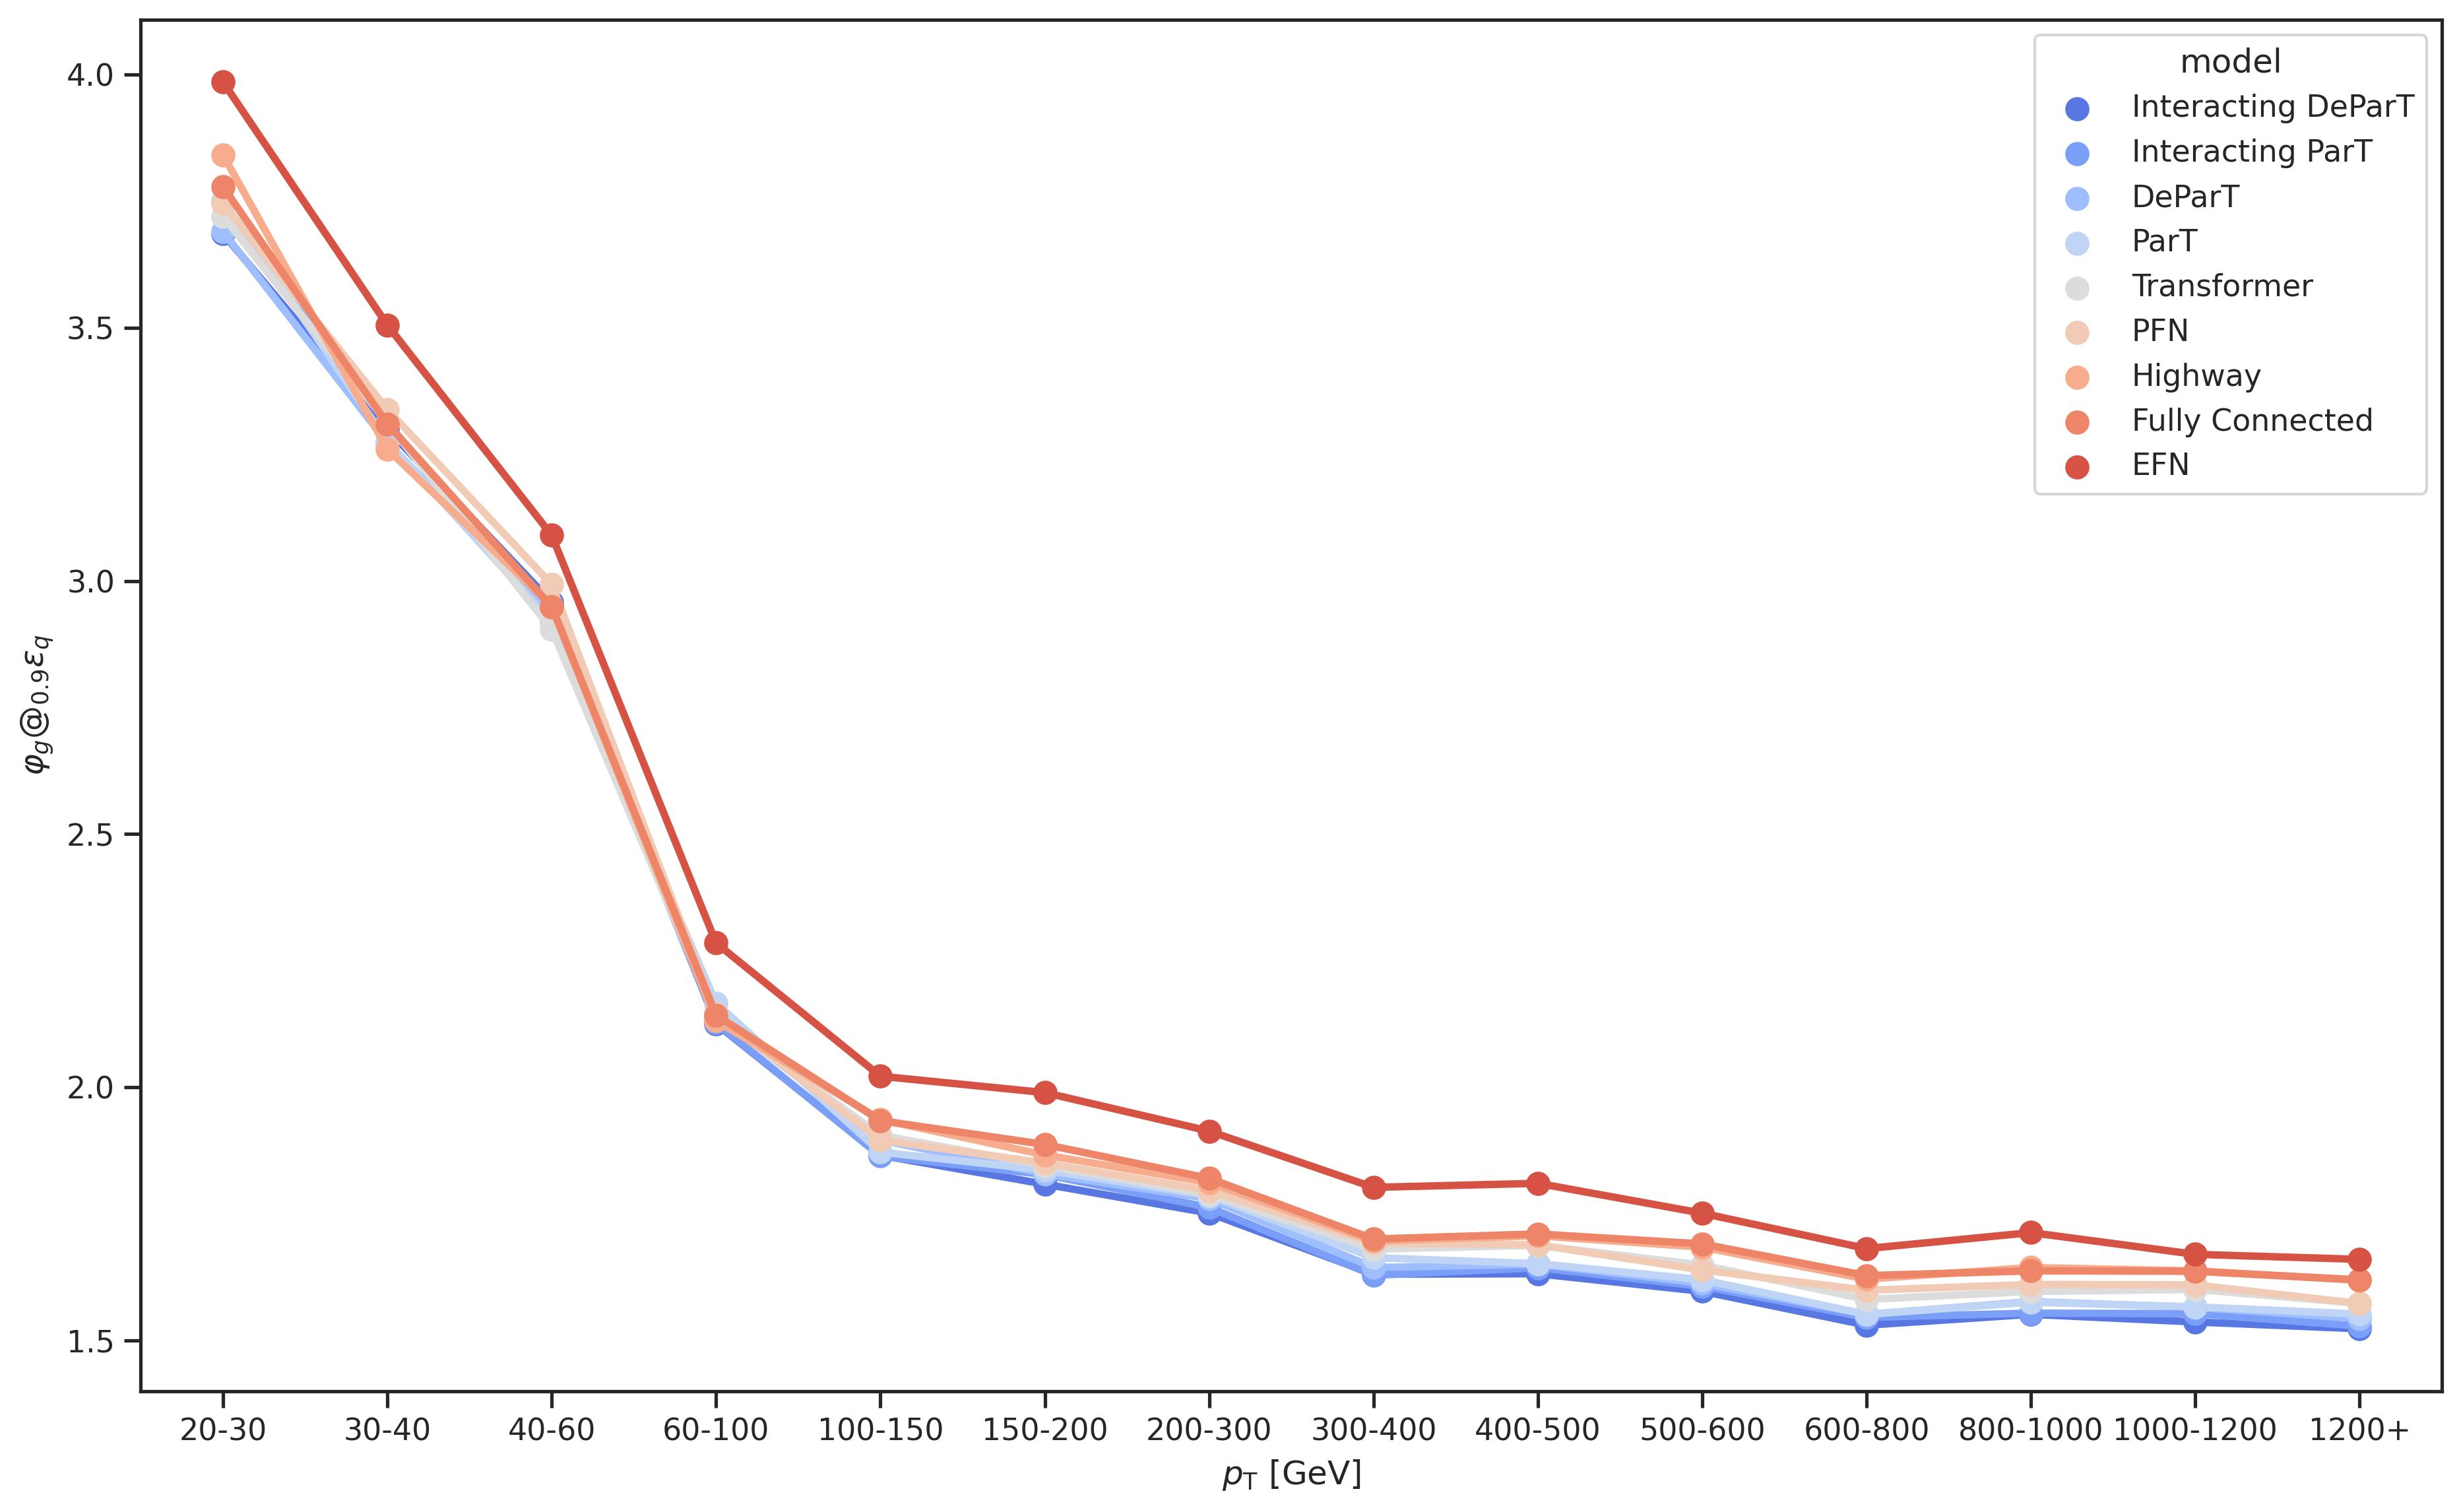
\includegraphics[width=0.95\linewidth]{src/plots/results/pT_dep/gluon_rej_at_quark_eff_0.9.jpg}
    \caption{Gluon rejection at quark efficiency of 0.9 as a function of transverse momentum.}
    \label{fig:gluon_rej_at_quark_eff_0.9_pt}
\end{figure}

\begin{figure}[htb]
    \centering
    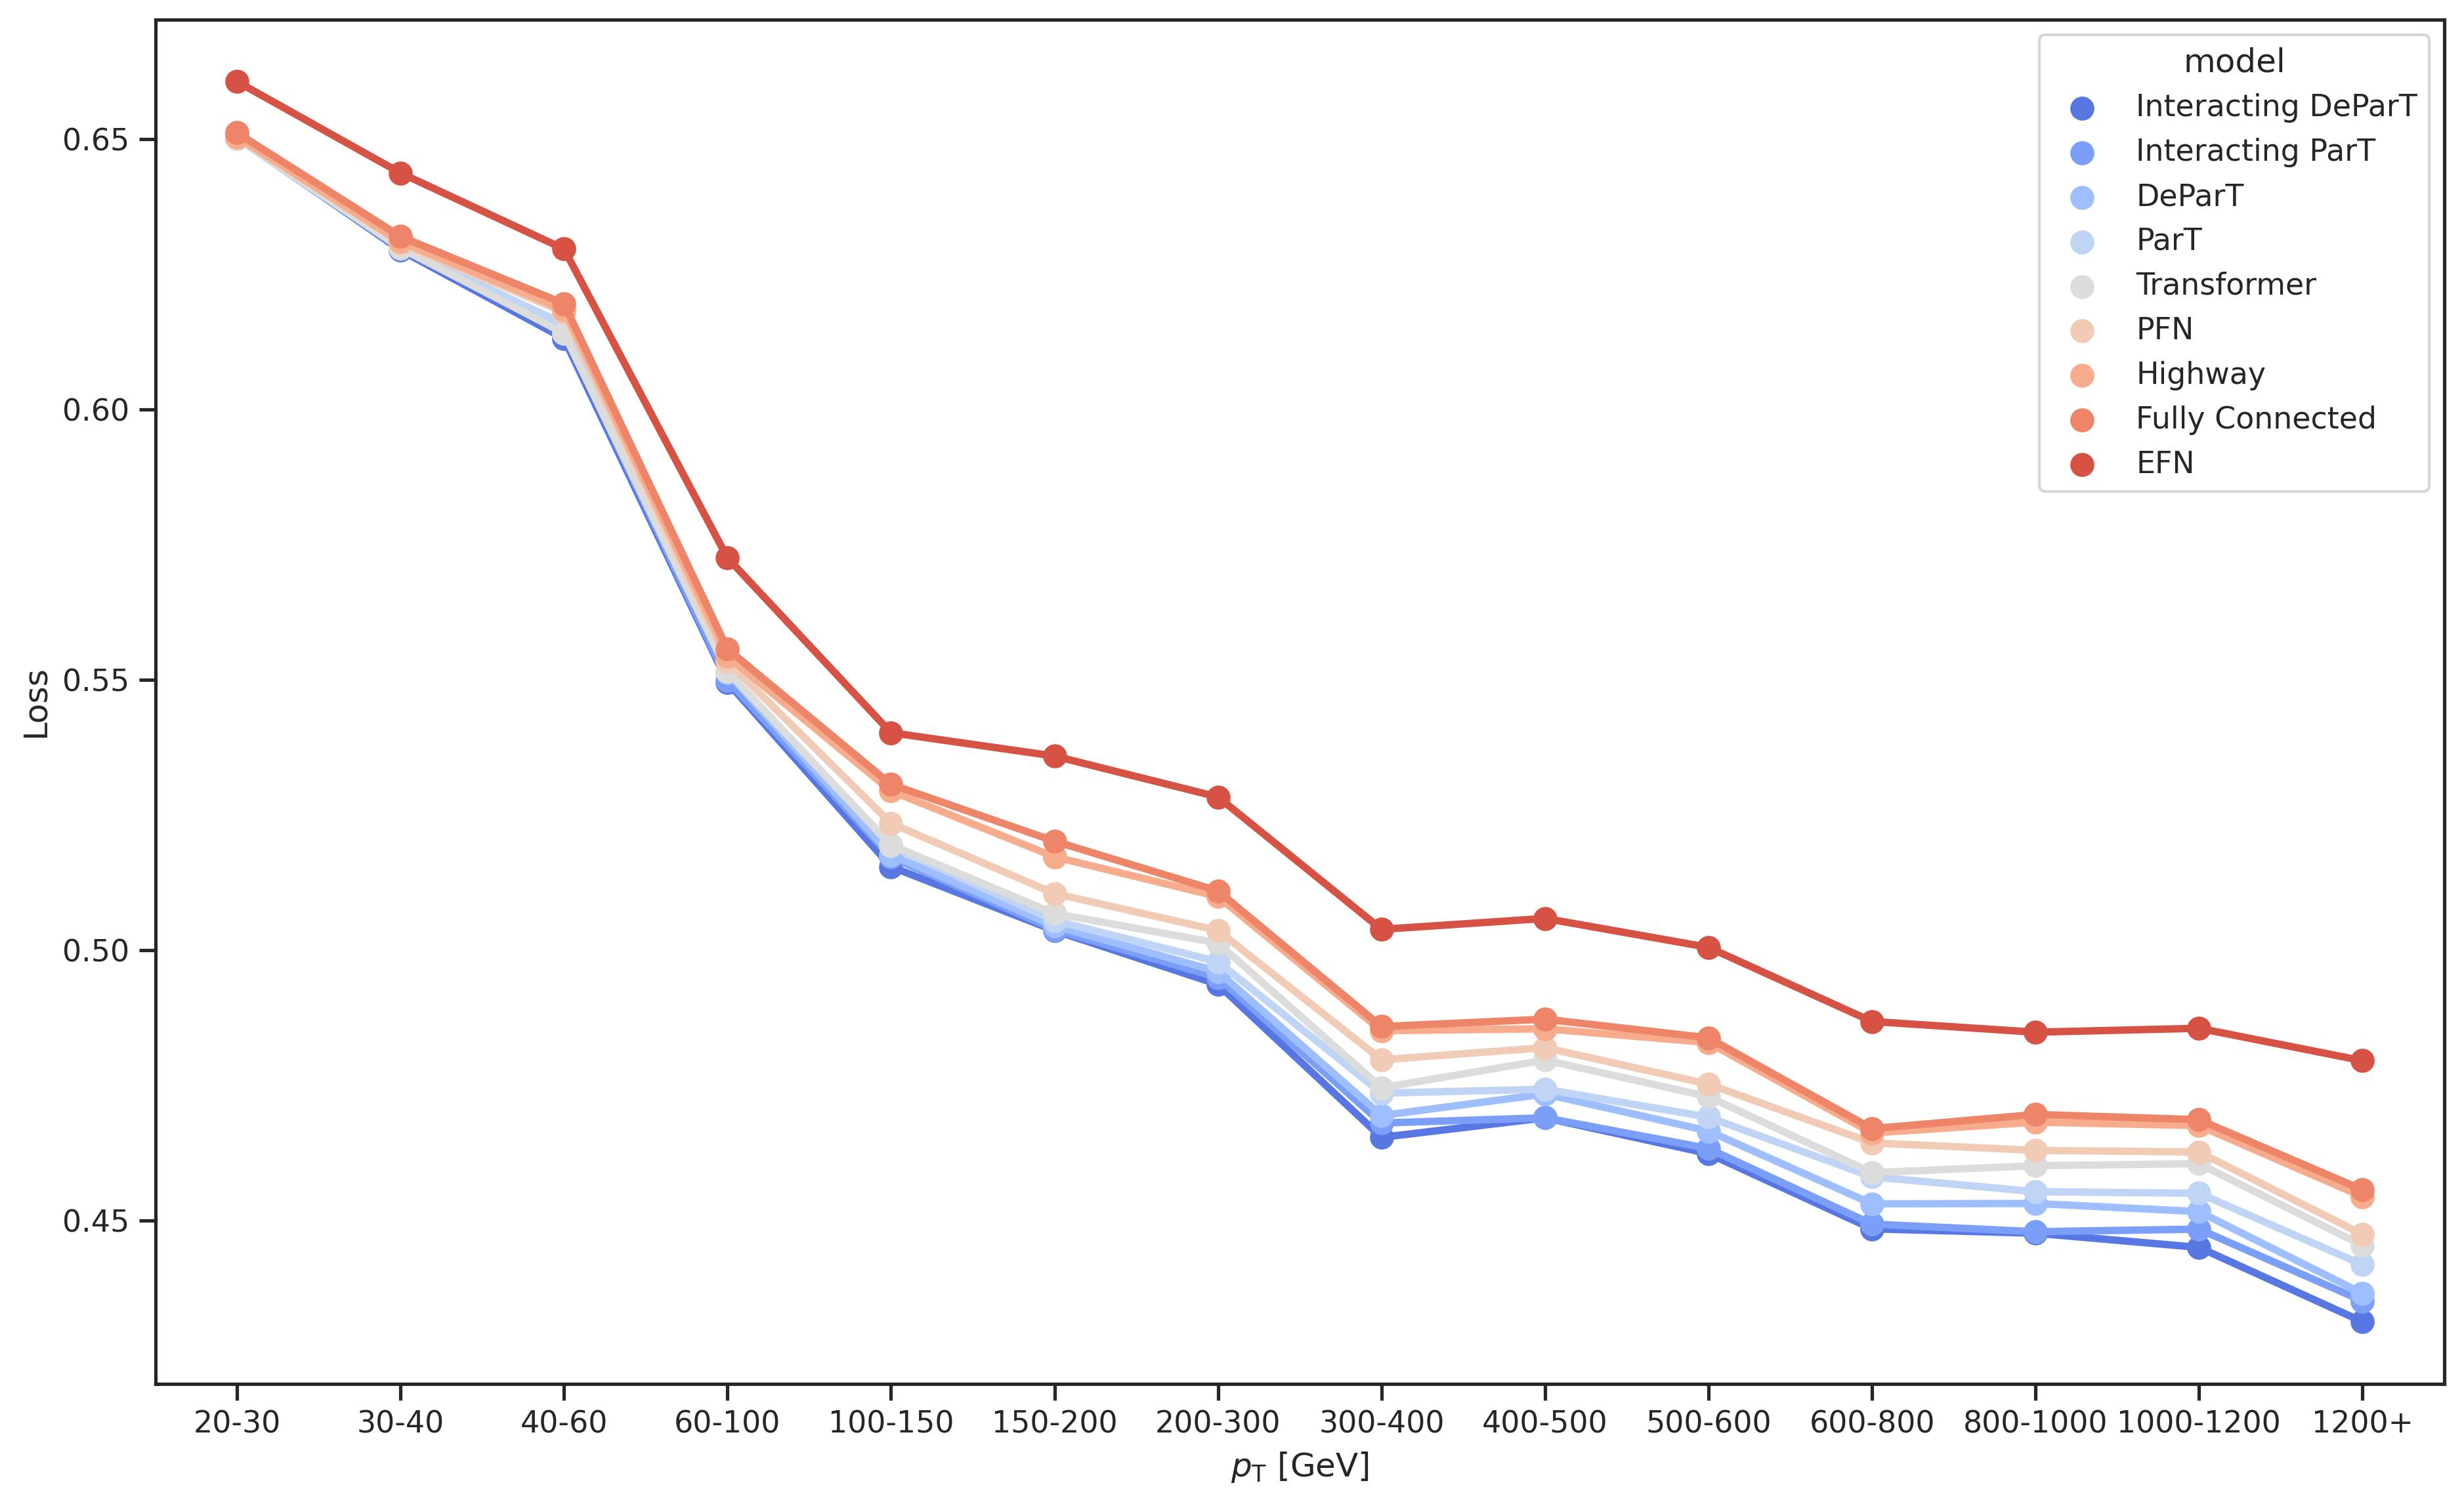
\includegraphics[width=0.95\linewidth]{src/plots/results/pT_dep/loss.jpg}
    \caption{Loss as a function of transverse momentum.}
    \label{fig:loss_pt}
\end{figure}

\FloatBarrier

\section{Pseudo-rapidity Dependence}
\label{sec:app_eta_dep}

\begin{figure}[htb]
    \centering
    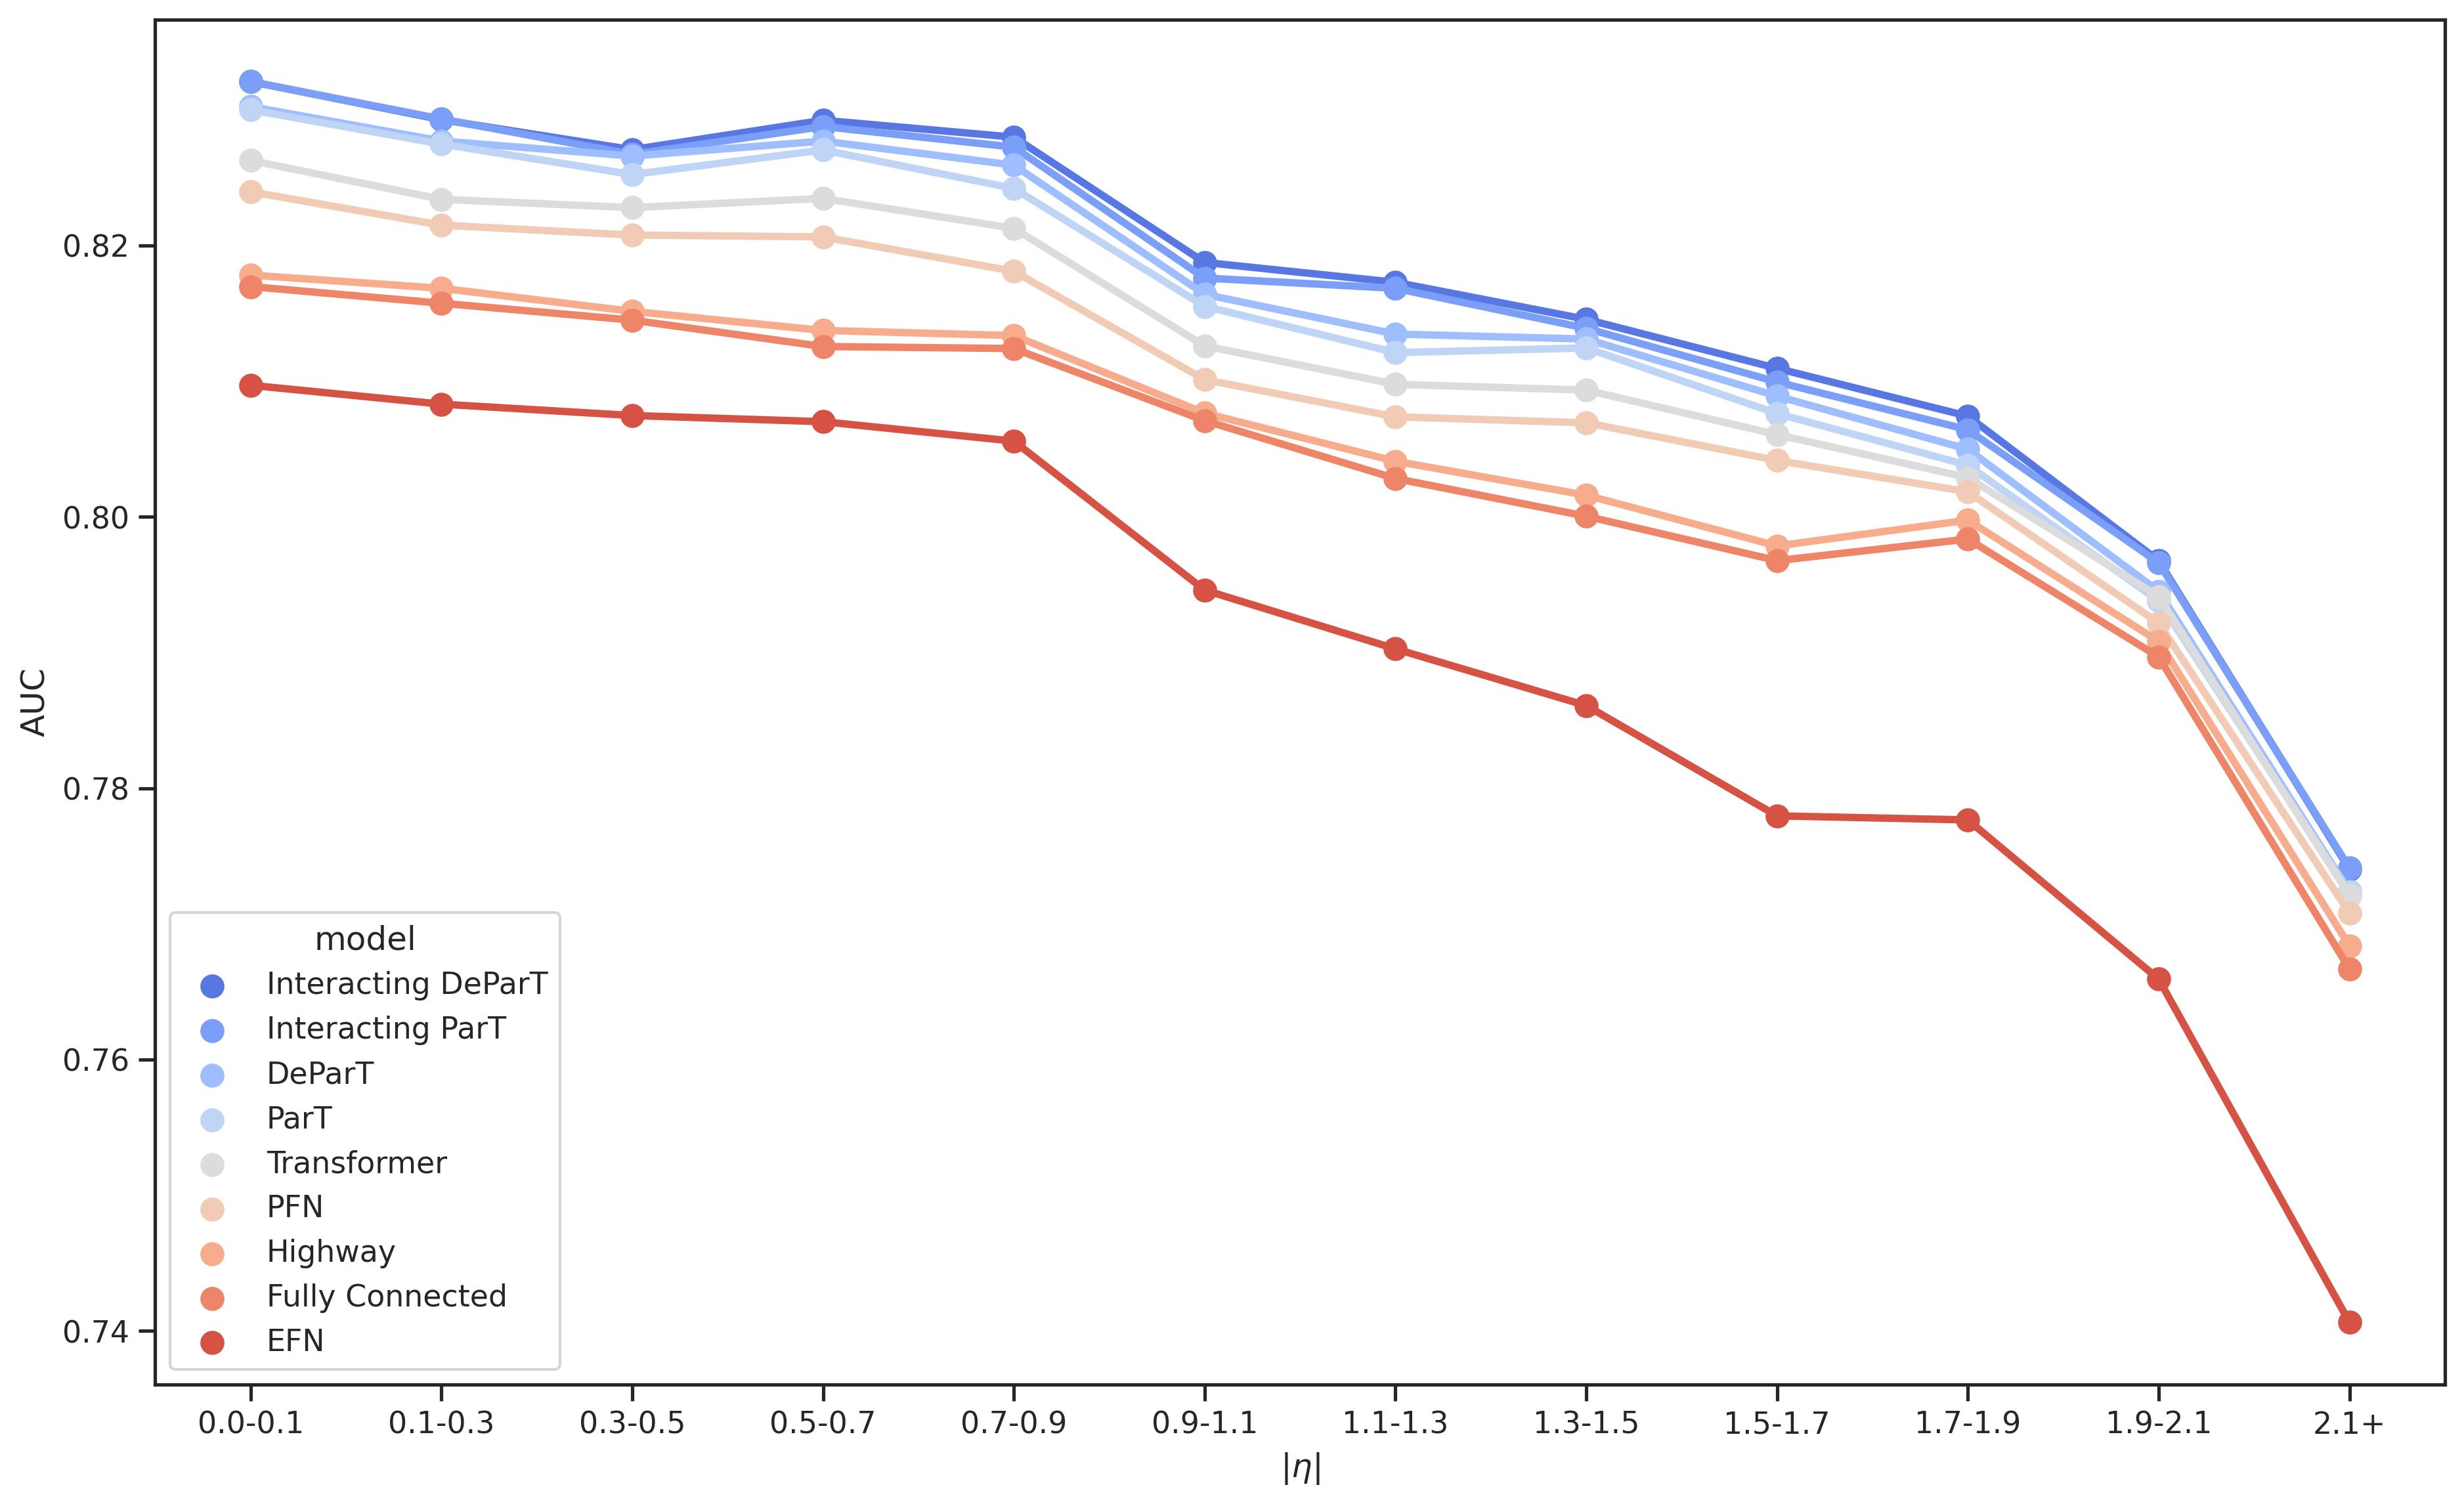
\includegraphics[width=0.95\linewidth]{src/plots/results/eta_dep/auc.jpg}
    \caption{AUC as a function of pseudo-rapidity.}
    \label{fig:auc_eta}
\end{figure}

\begin{figure}[htb]
    \centering
    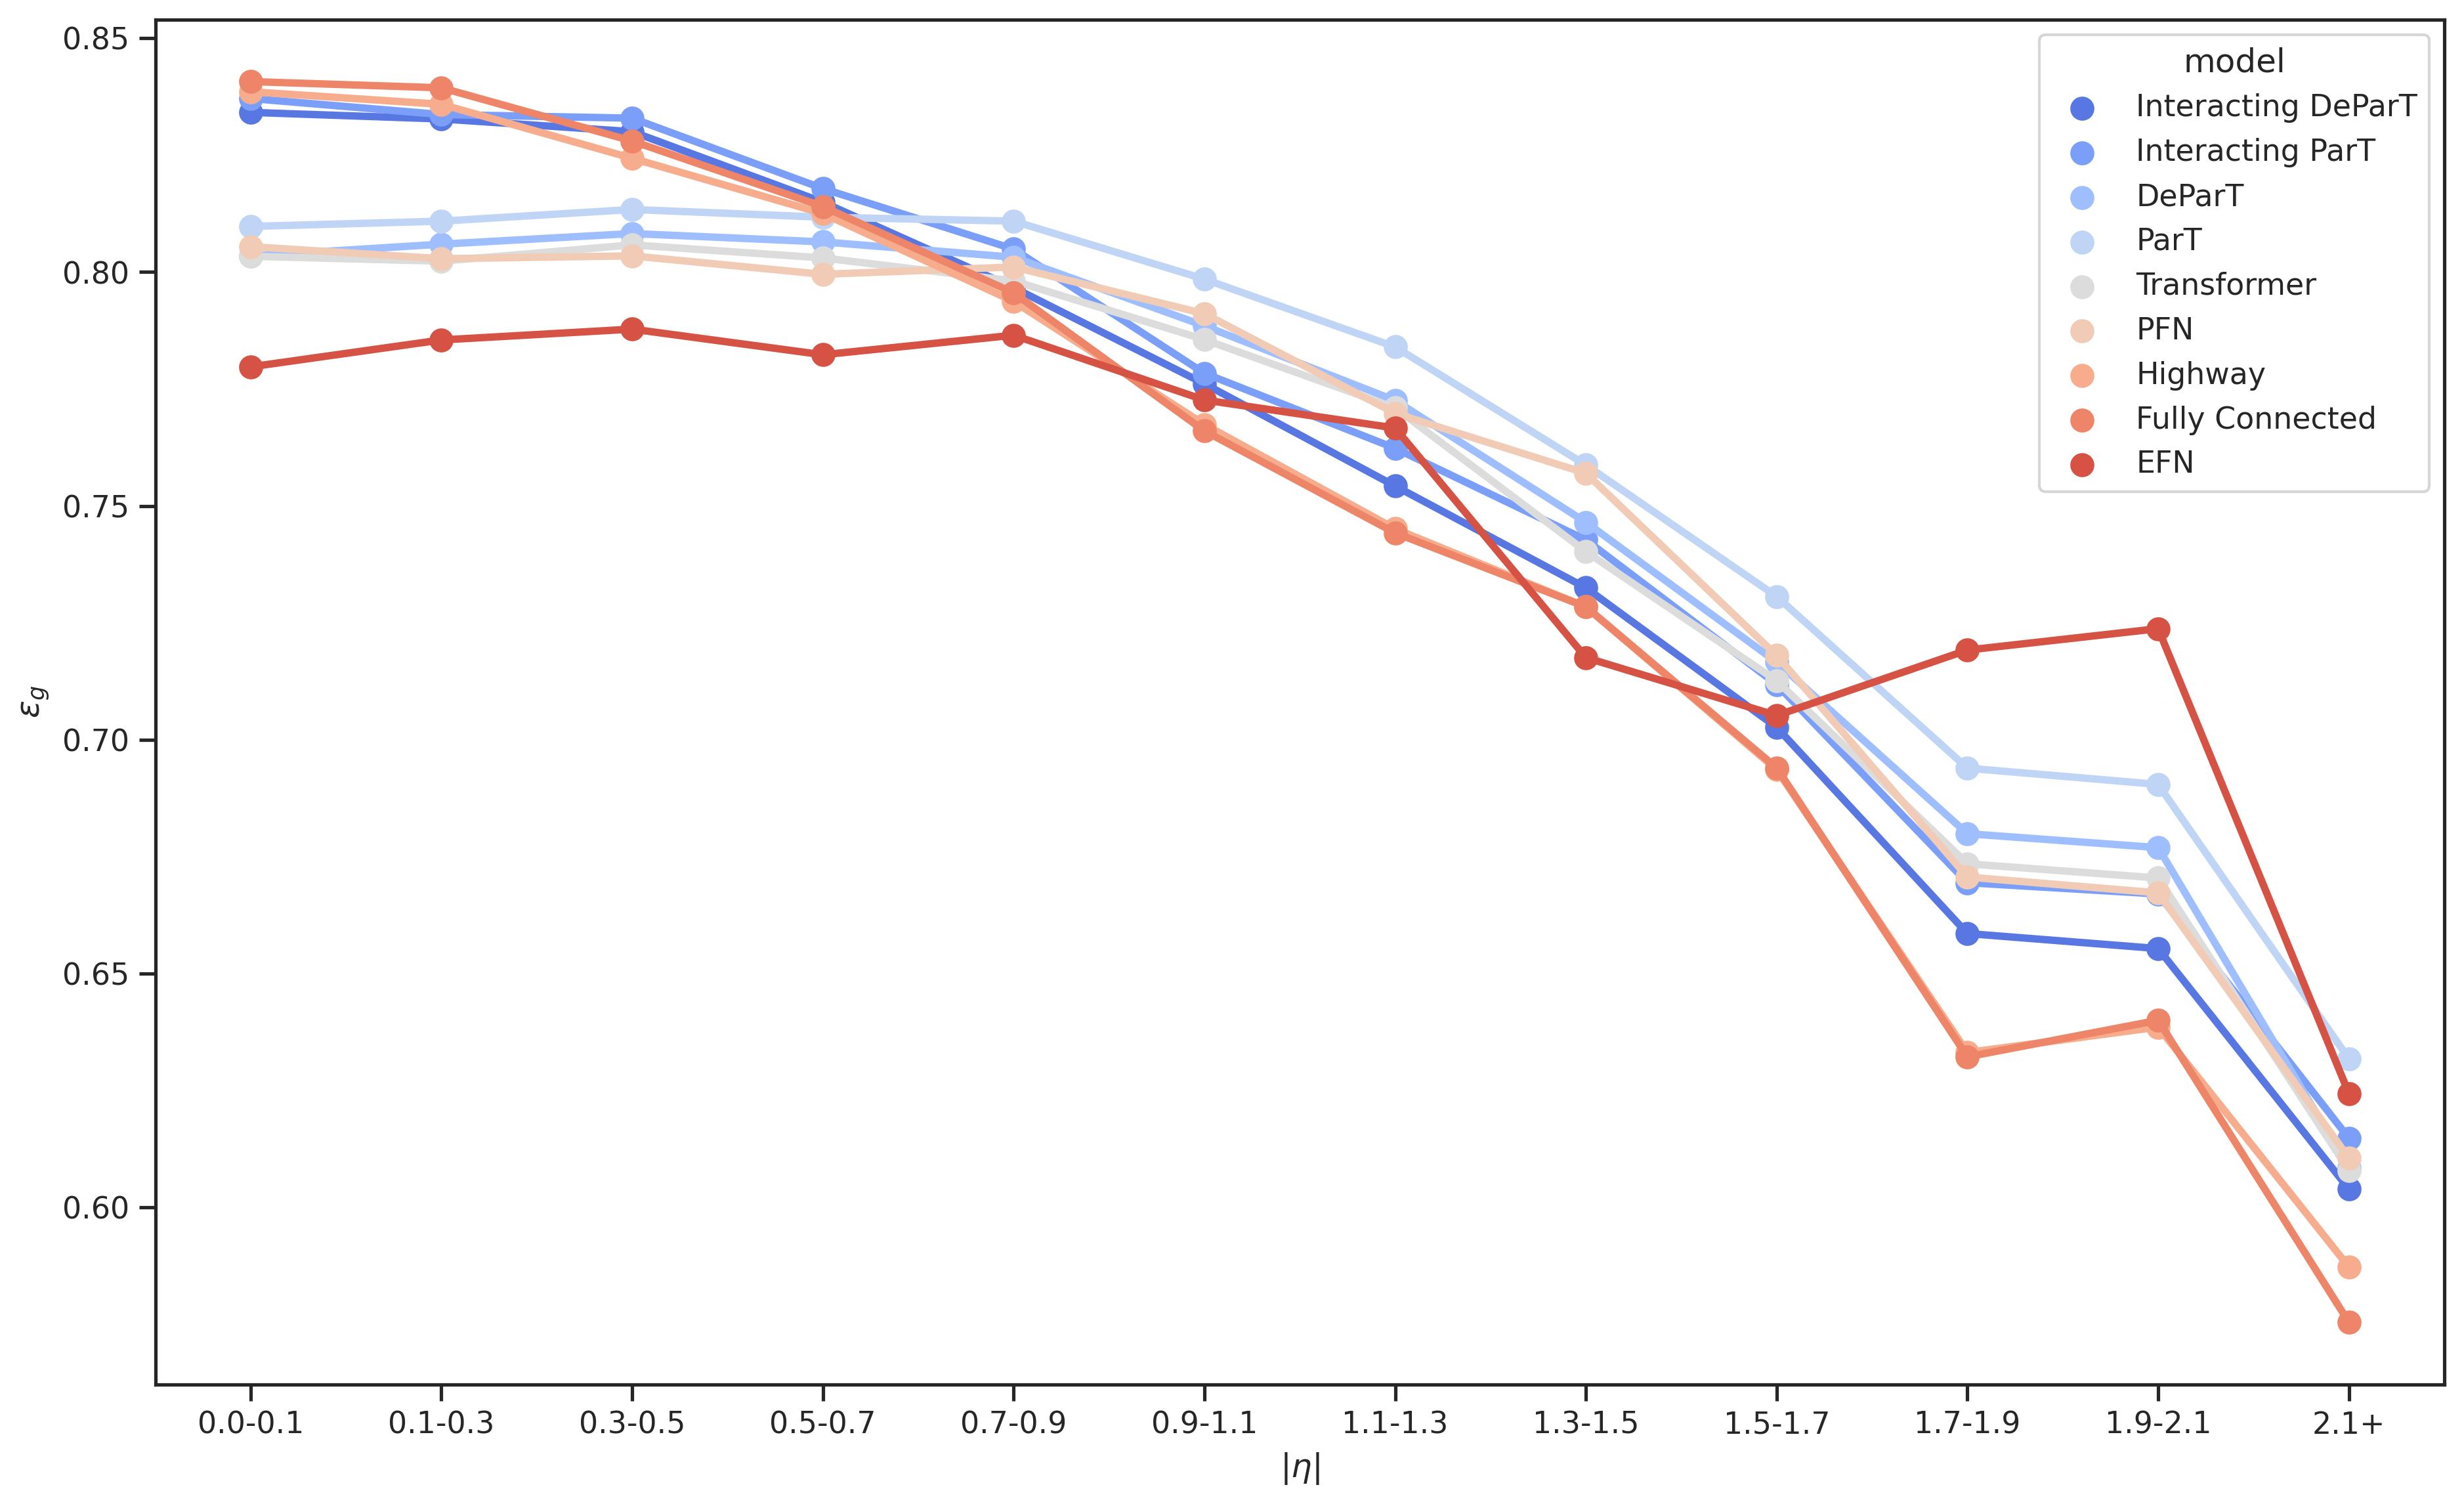
\includegraphics[width=0.95\linewidth]{src/plots/results/eta_dep/gluon_efficiency.jpg}
    \caption{Gluon efficiency as a function of pseudo-rapidity.}
    \label{fig:gluon_eff_eta}
\end{figure}

\begin{figure}[htb]
    \centering
    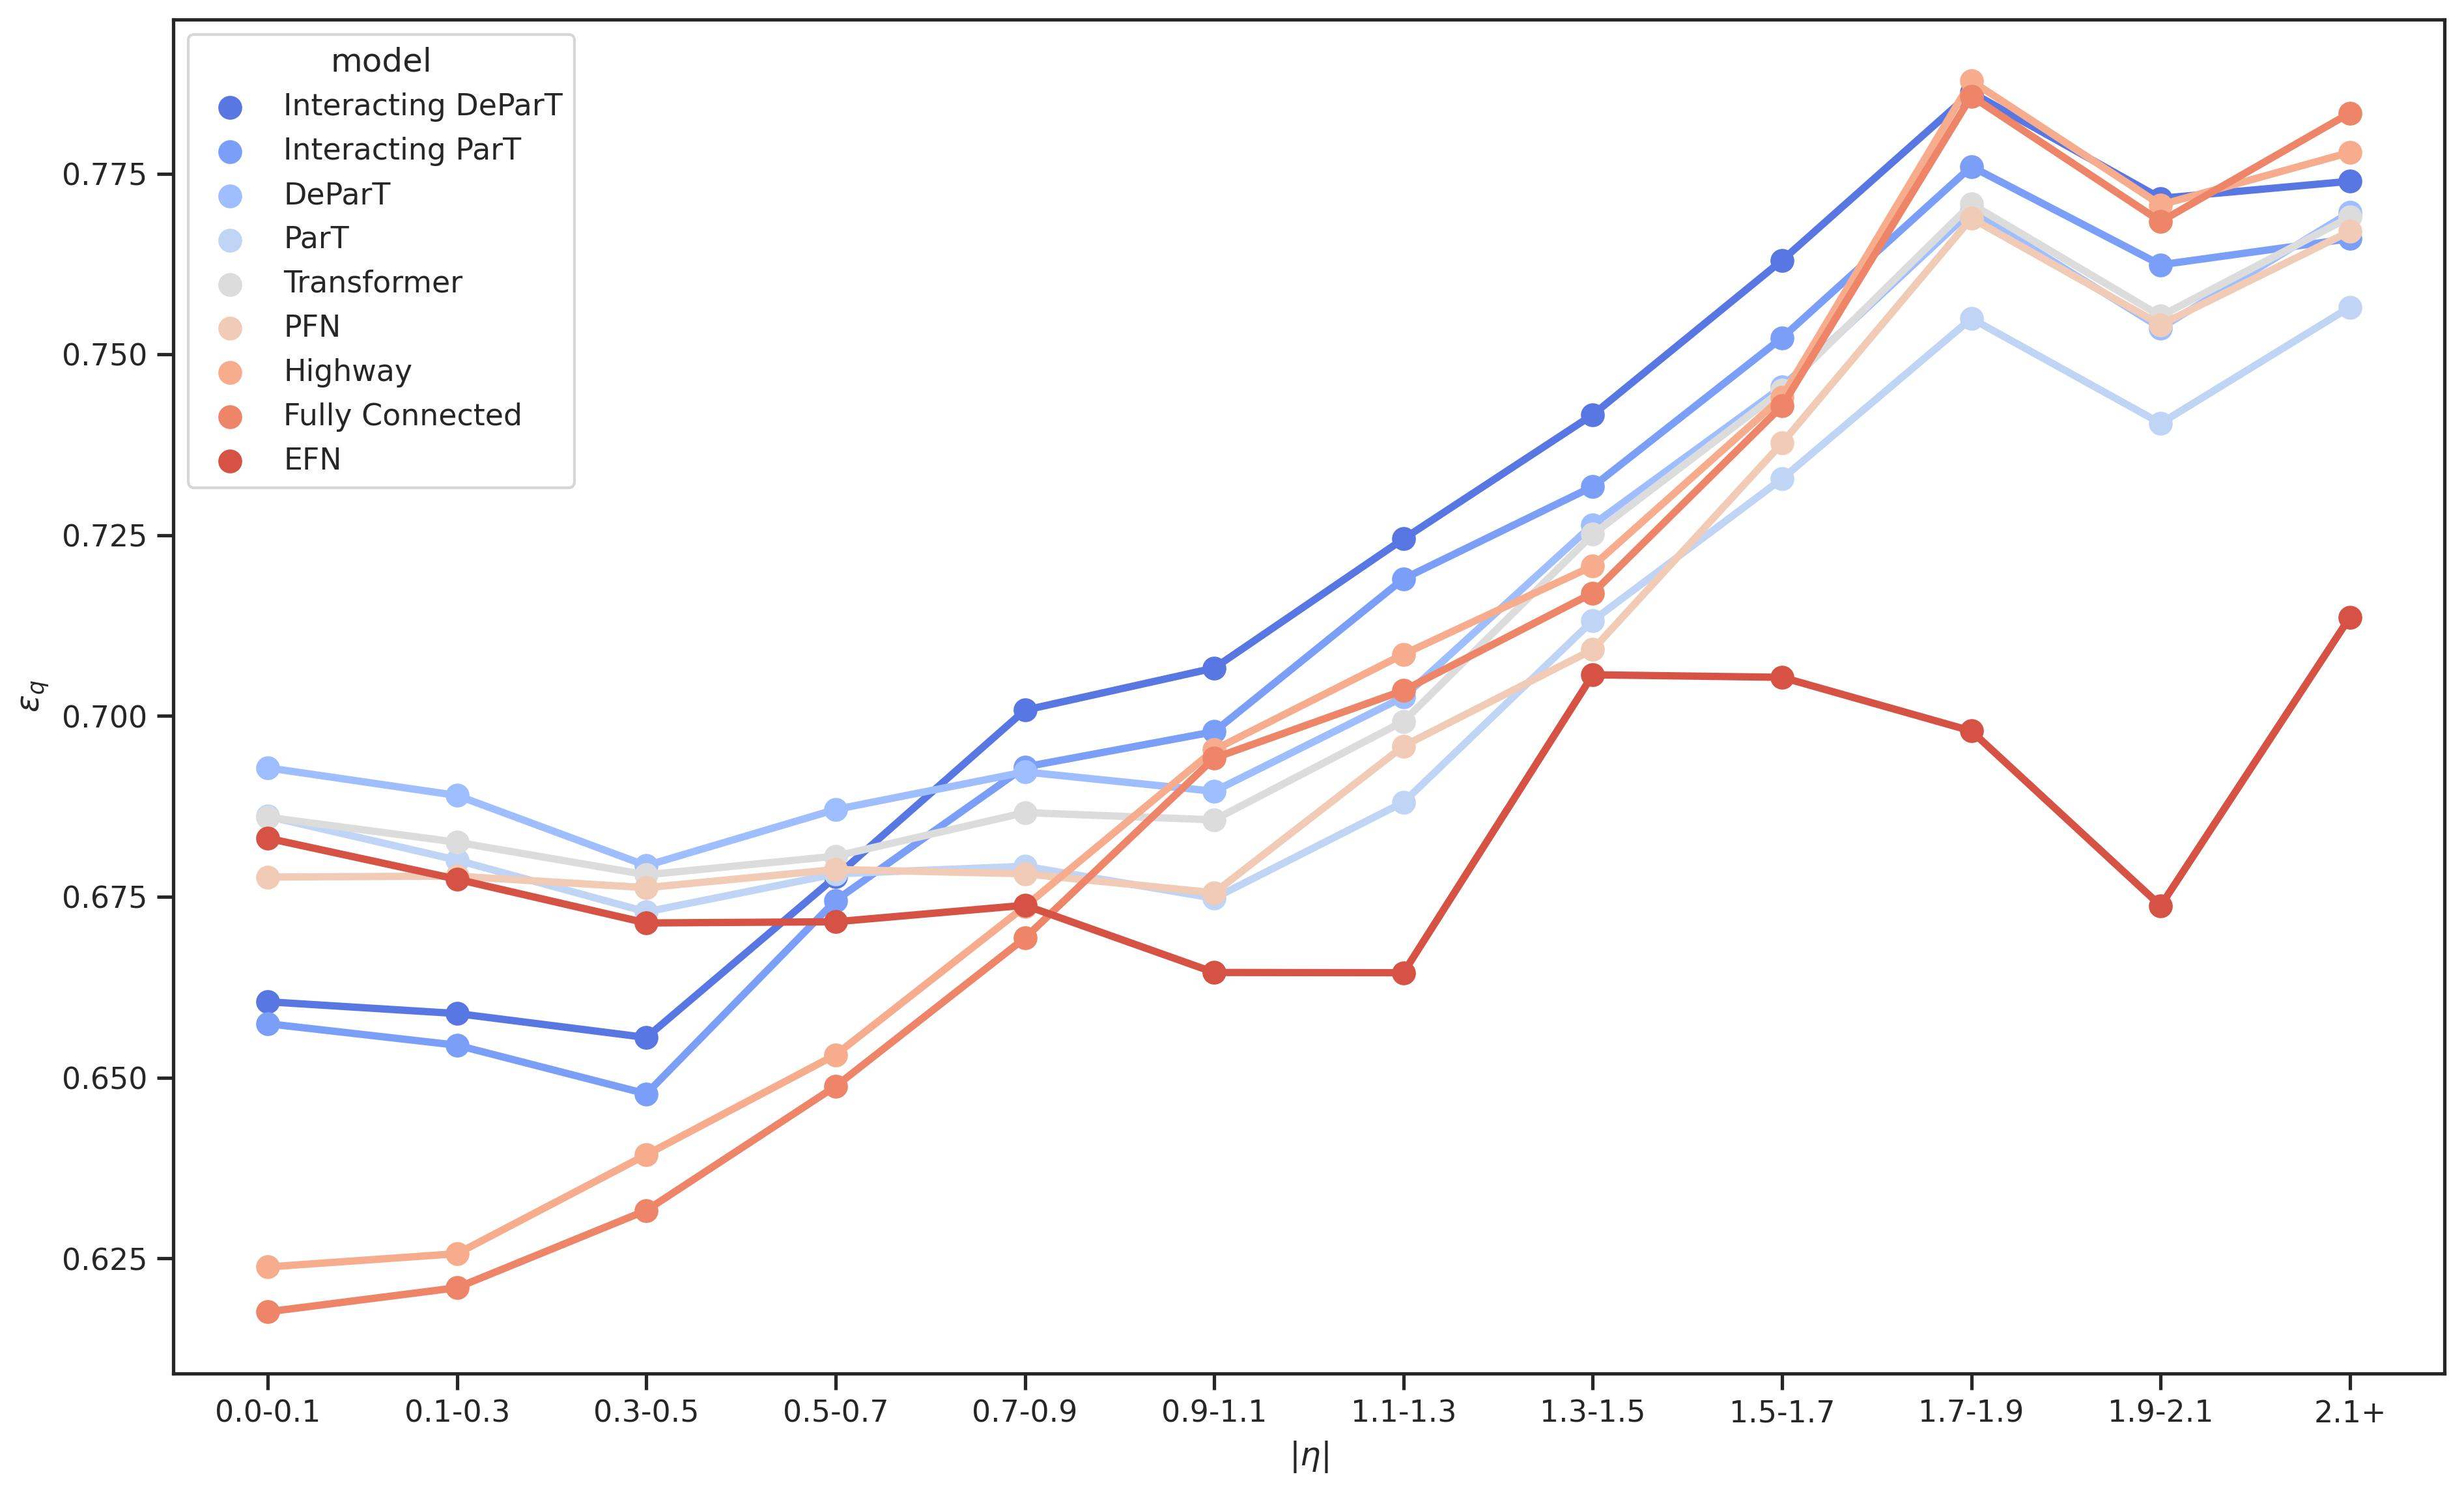
\includegraphics[width=0.95\linewidth]{src/plots/results/eta_dep/quark_efficiency.jpg}
    \caption{Quark efficiency as a function of pseudo-rapidity.}
    \label{fig:quark_eff_eta}
\end{figure}

\begin{figure}[htb]
    \centering
    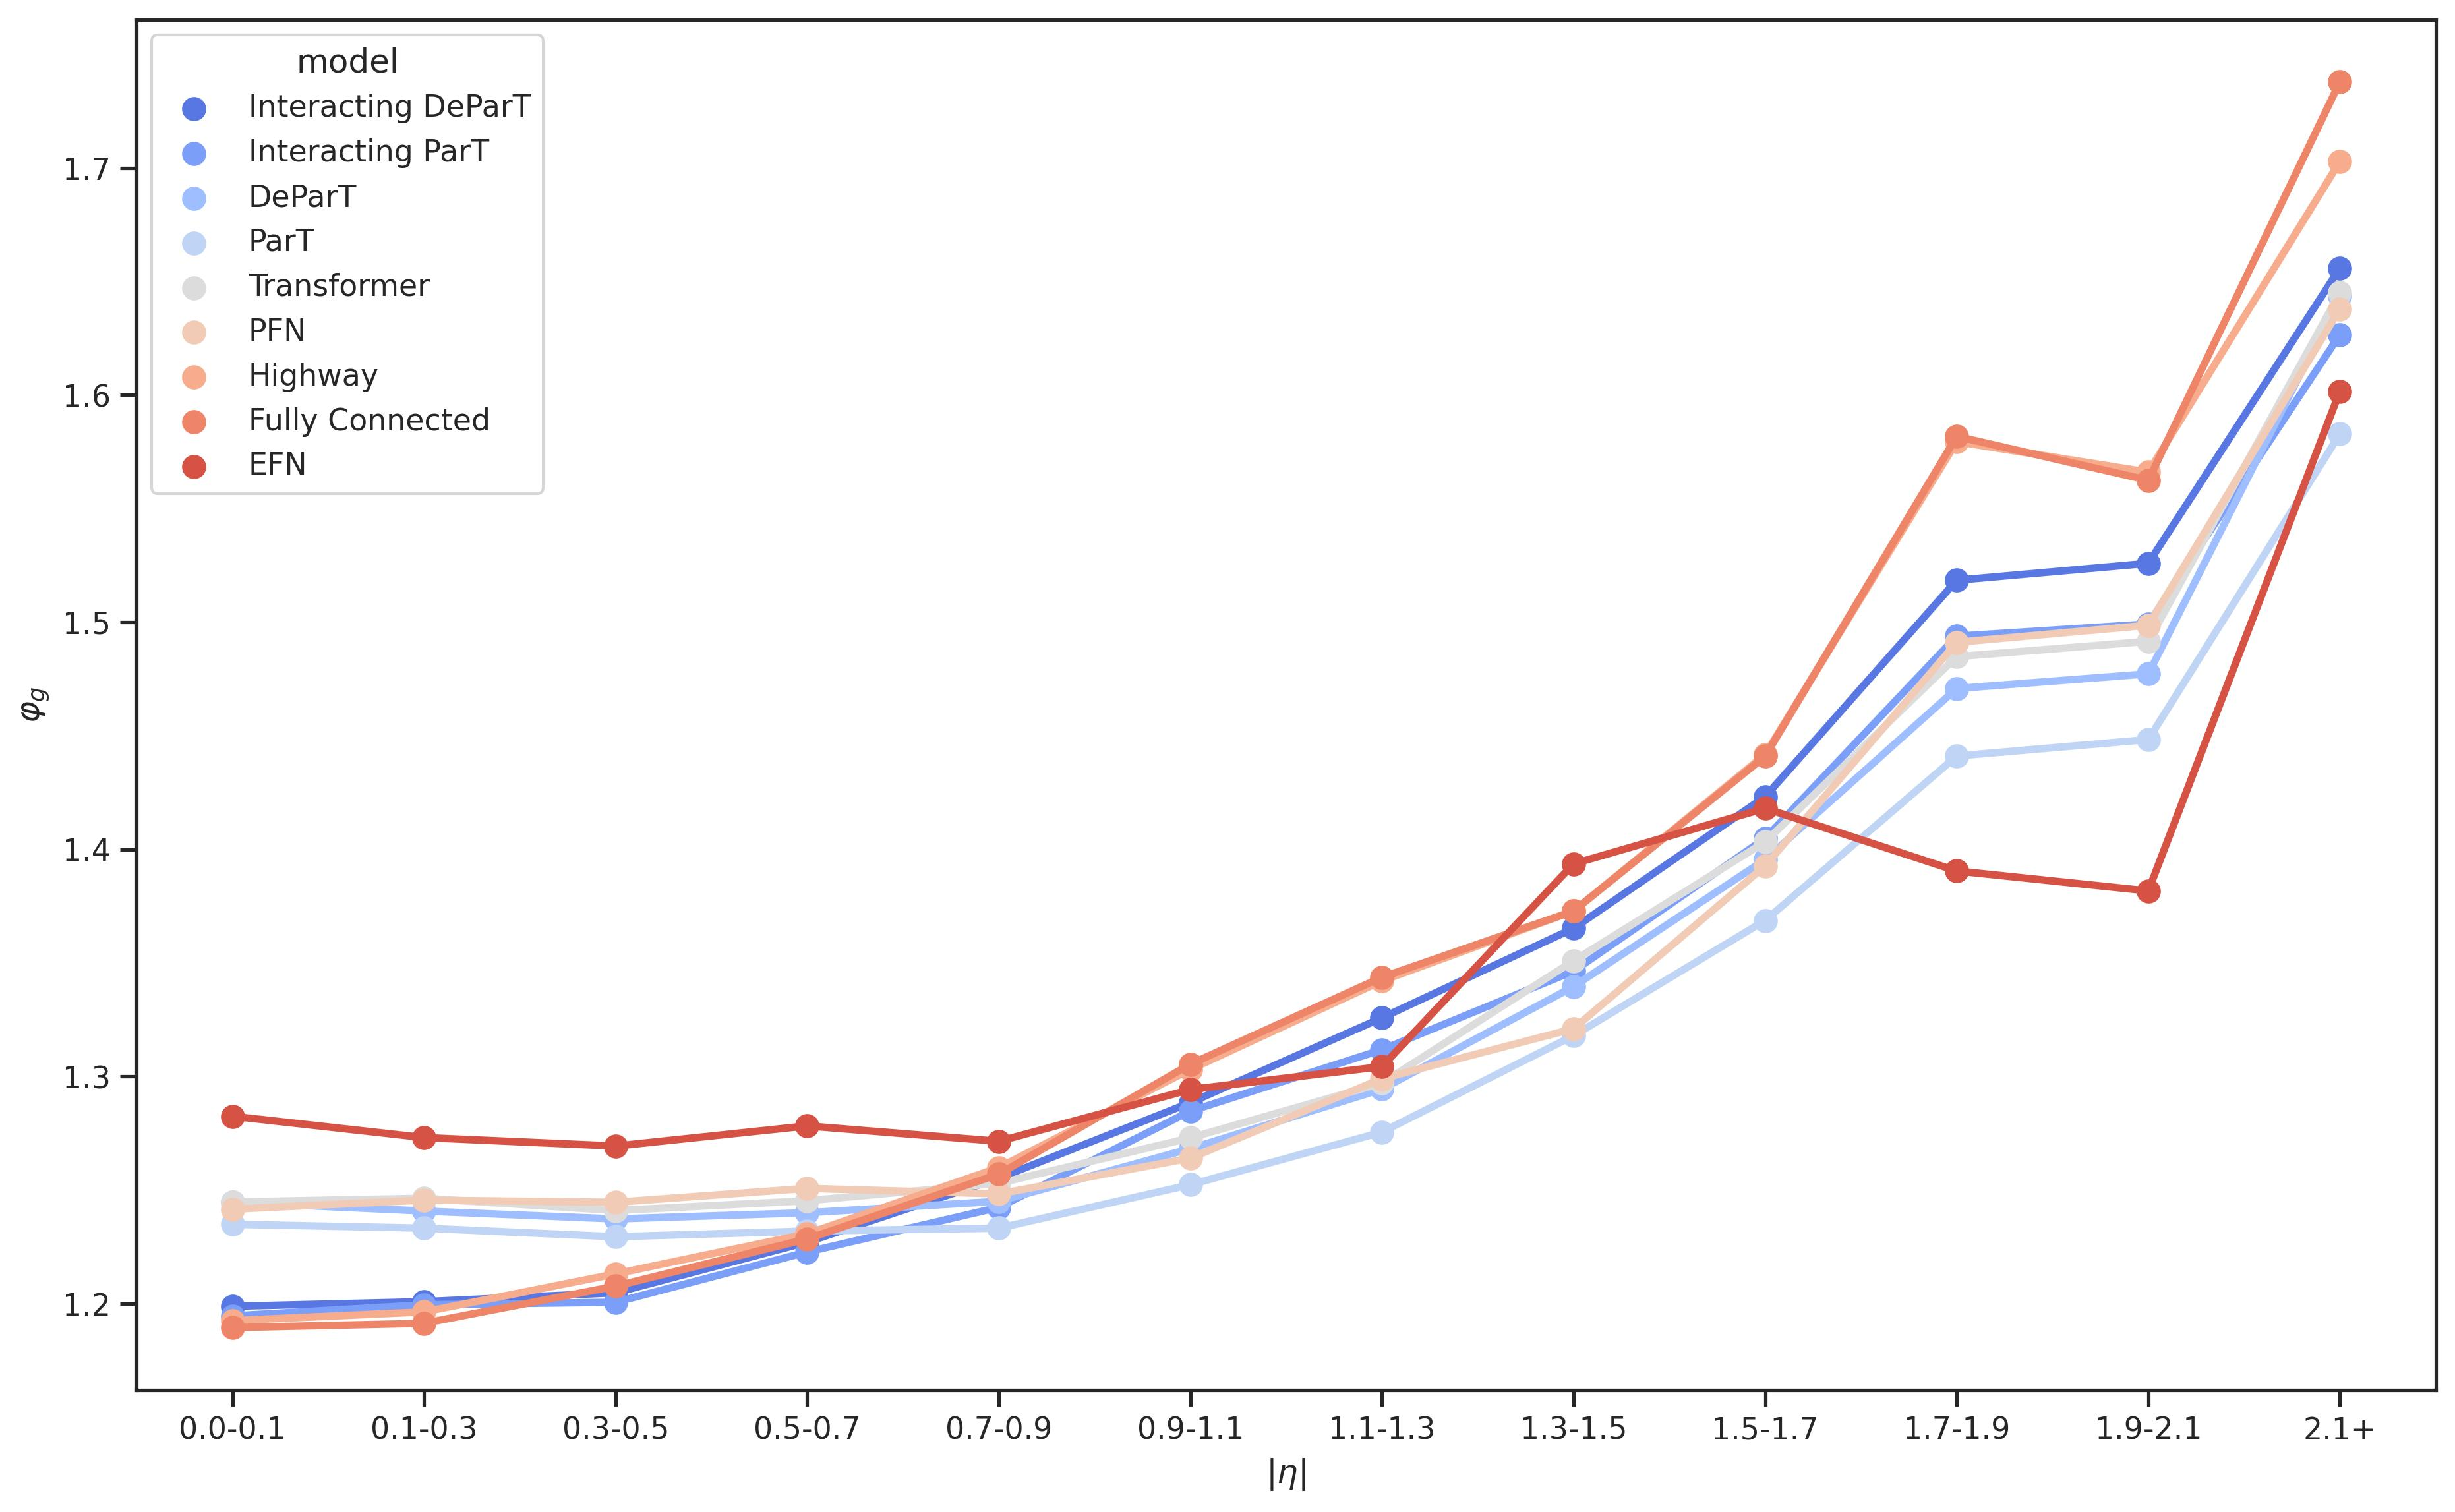
\includegraphics[width=0.95\linewidth]{src/plots/results/eta_dep/gluon_rejection.jpg}
    \caption{Gluon rejection as a function of pseudo-rapidity.}
    \label{fig:gluon_rej_eta}
\end{figure}

\begin{figure}[htb]
    \centering
    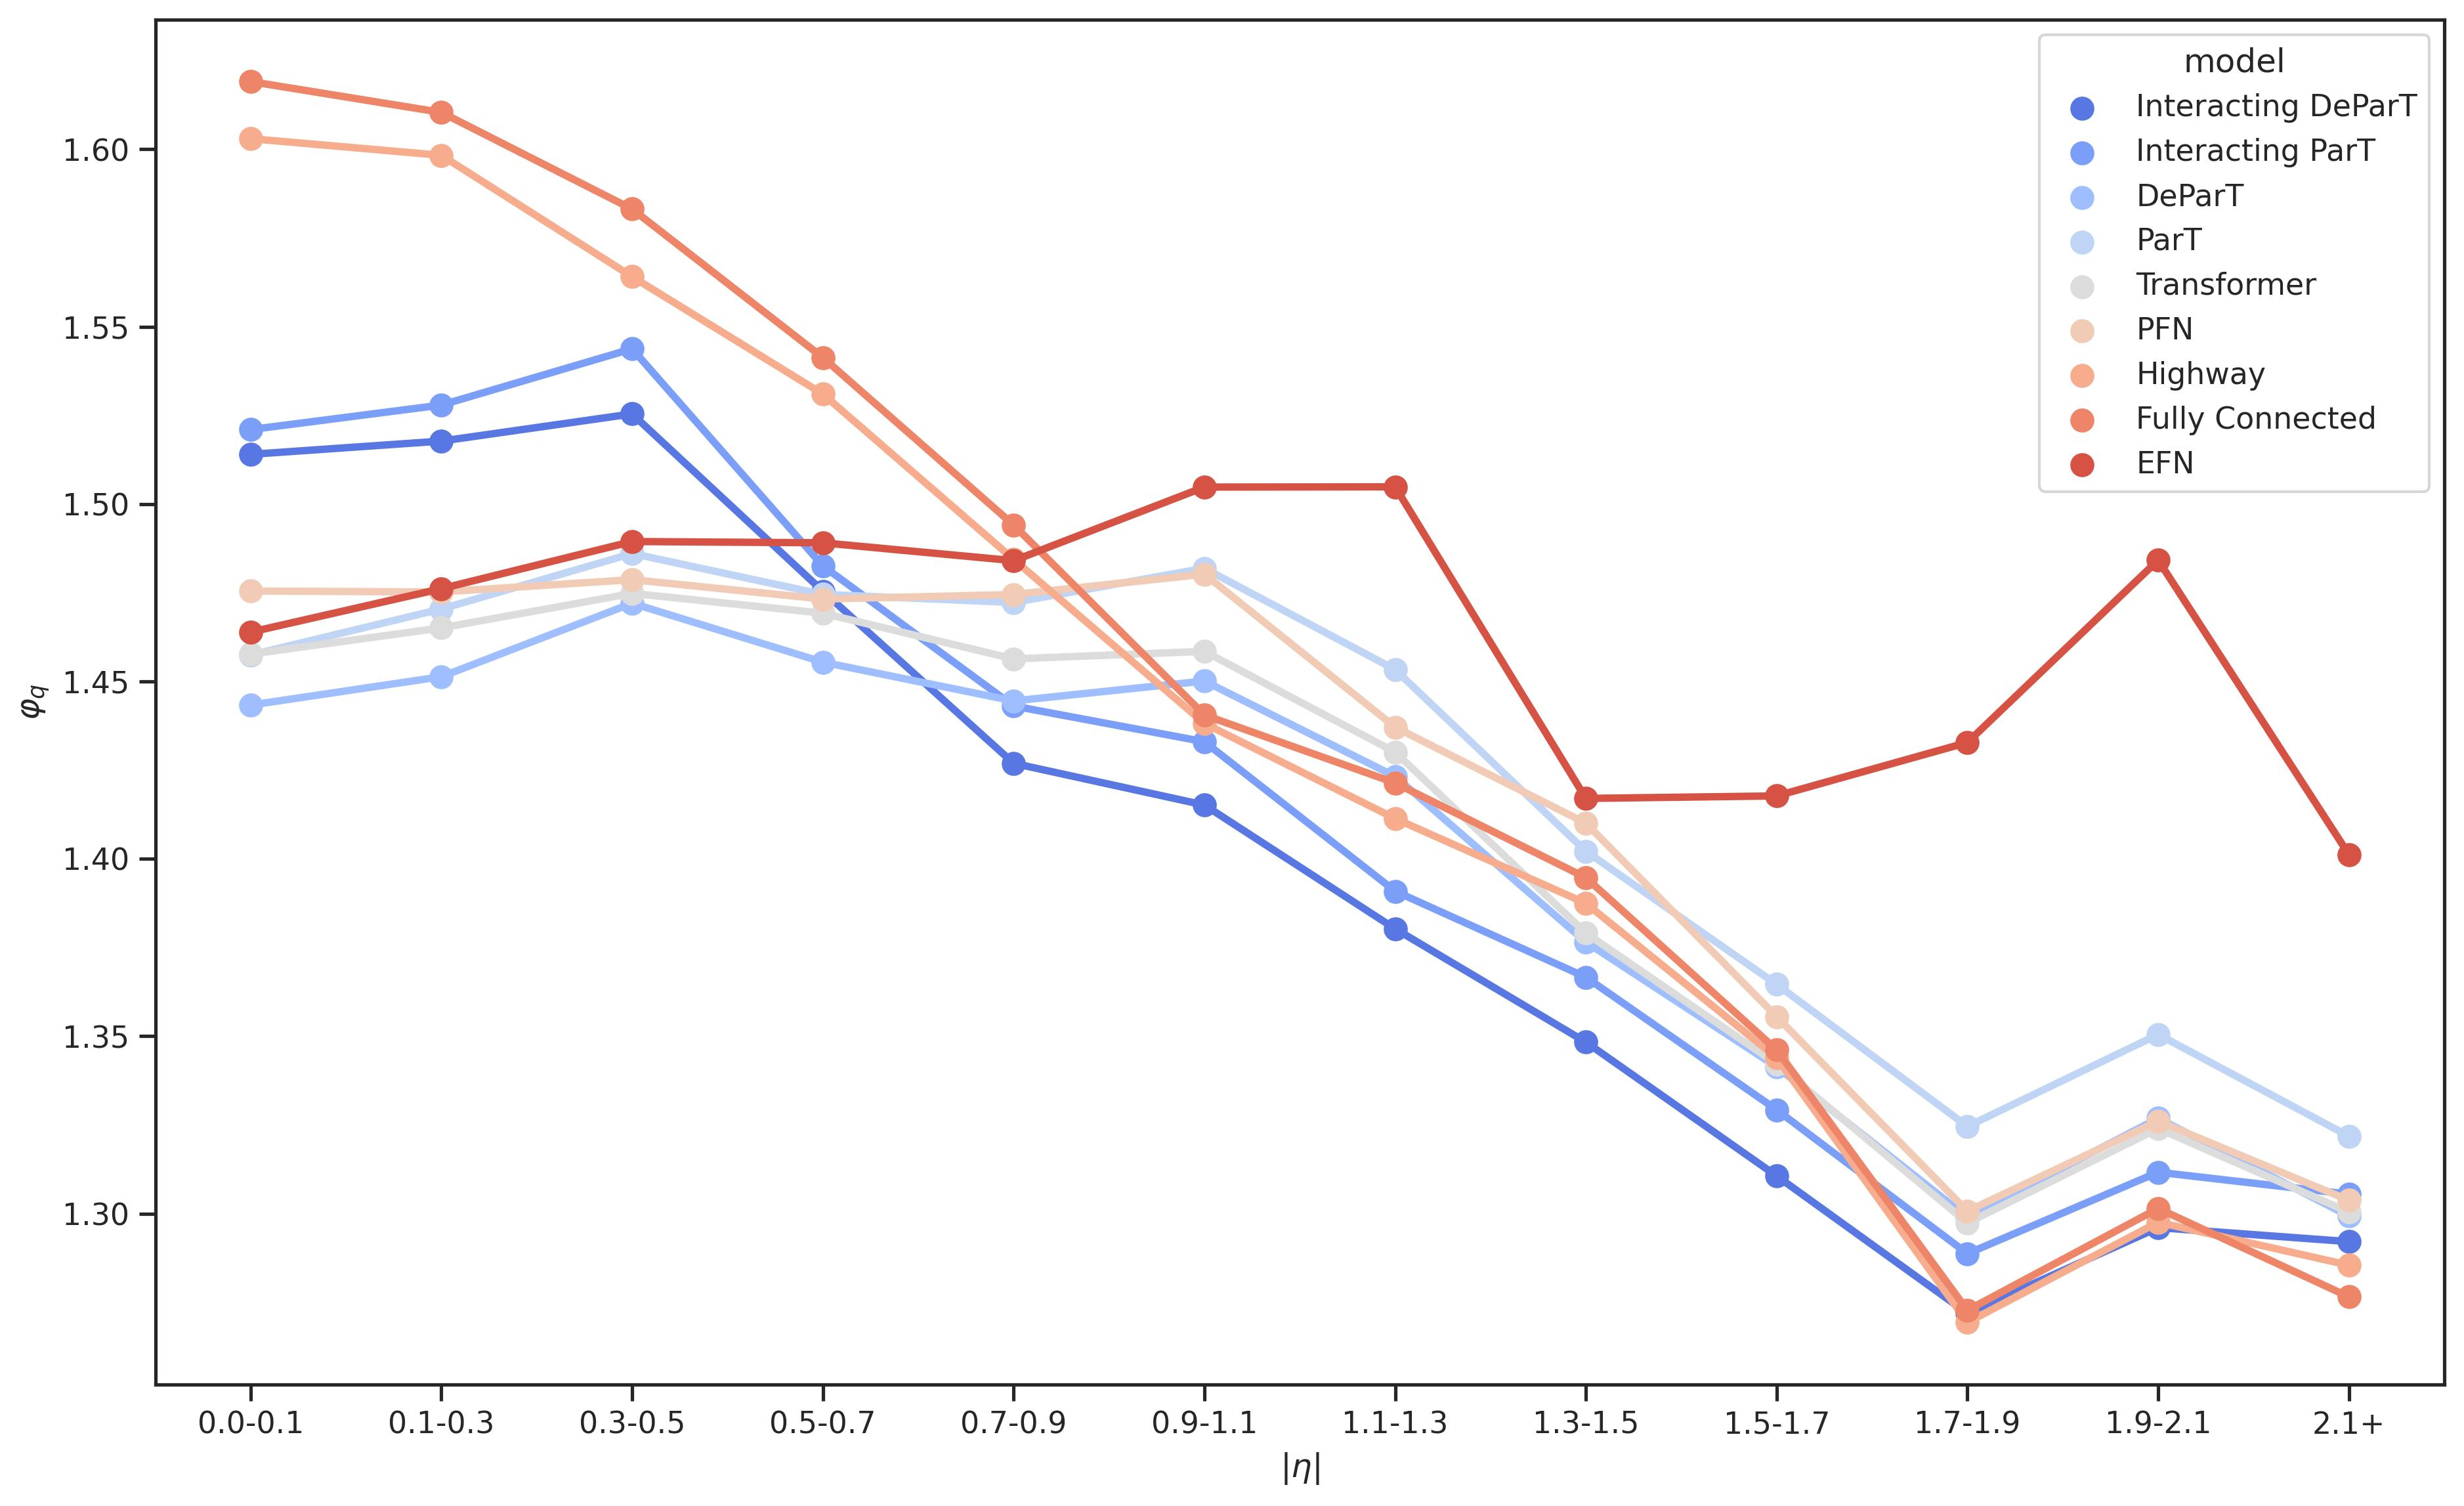
\includegraphics[width=0.95\linewidth]{src/plots/results/eta_dep/quark_rejection.jpg}
    \caption{Quark rejection as a function of pseudo-rapidity.}
    \label{fig:quark_rej_eta}
\end{figure}

\begin{figure}[htb]
    \centering
    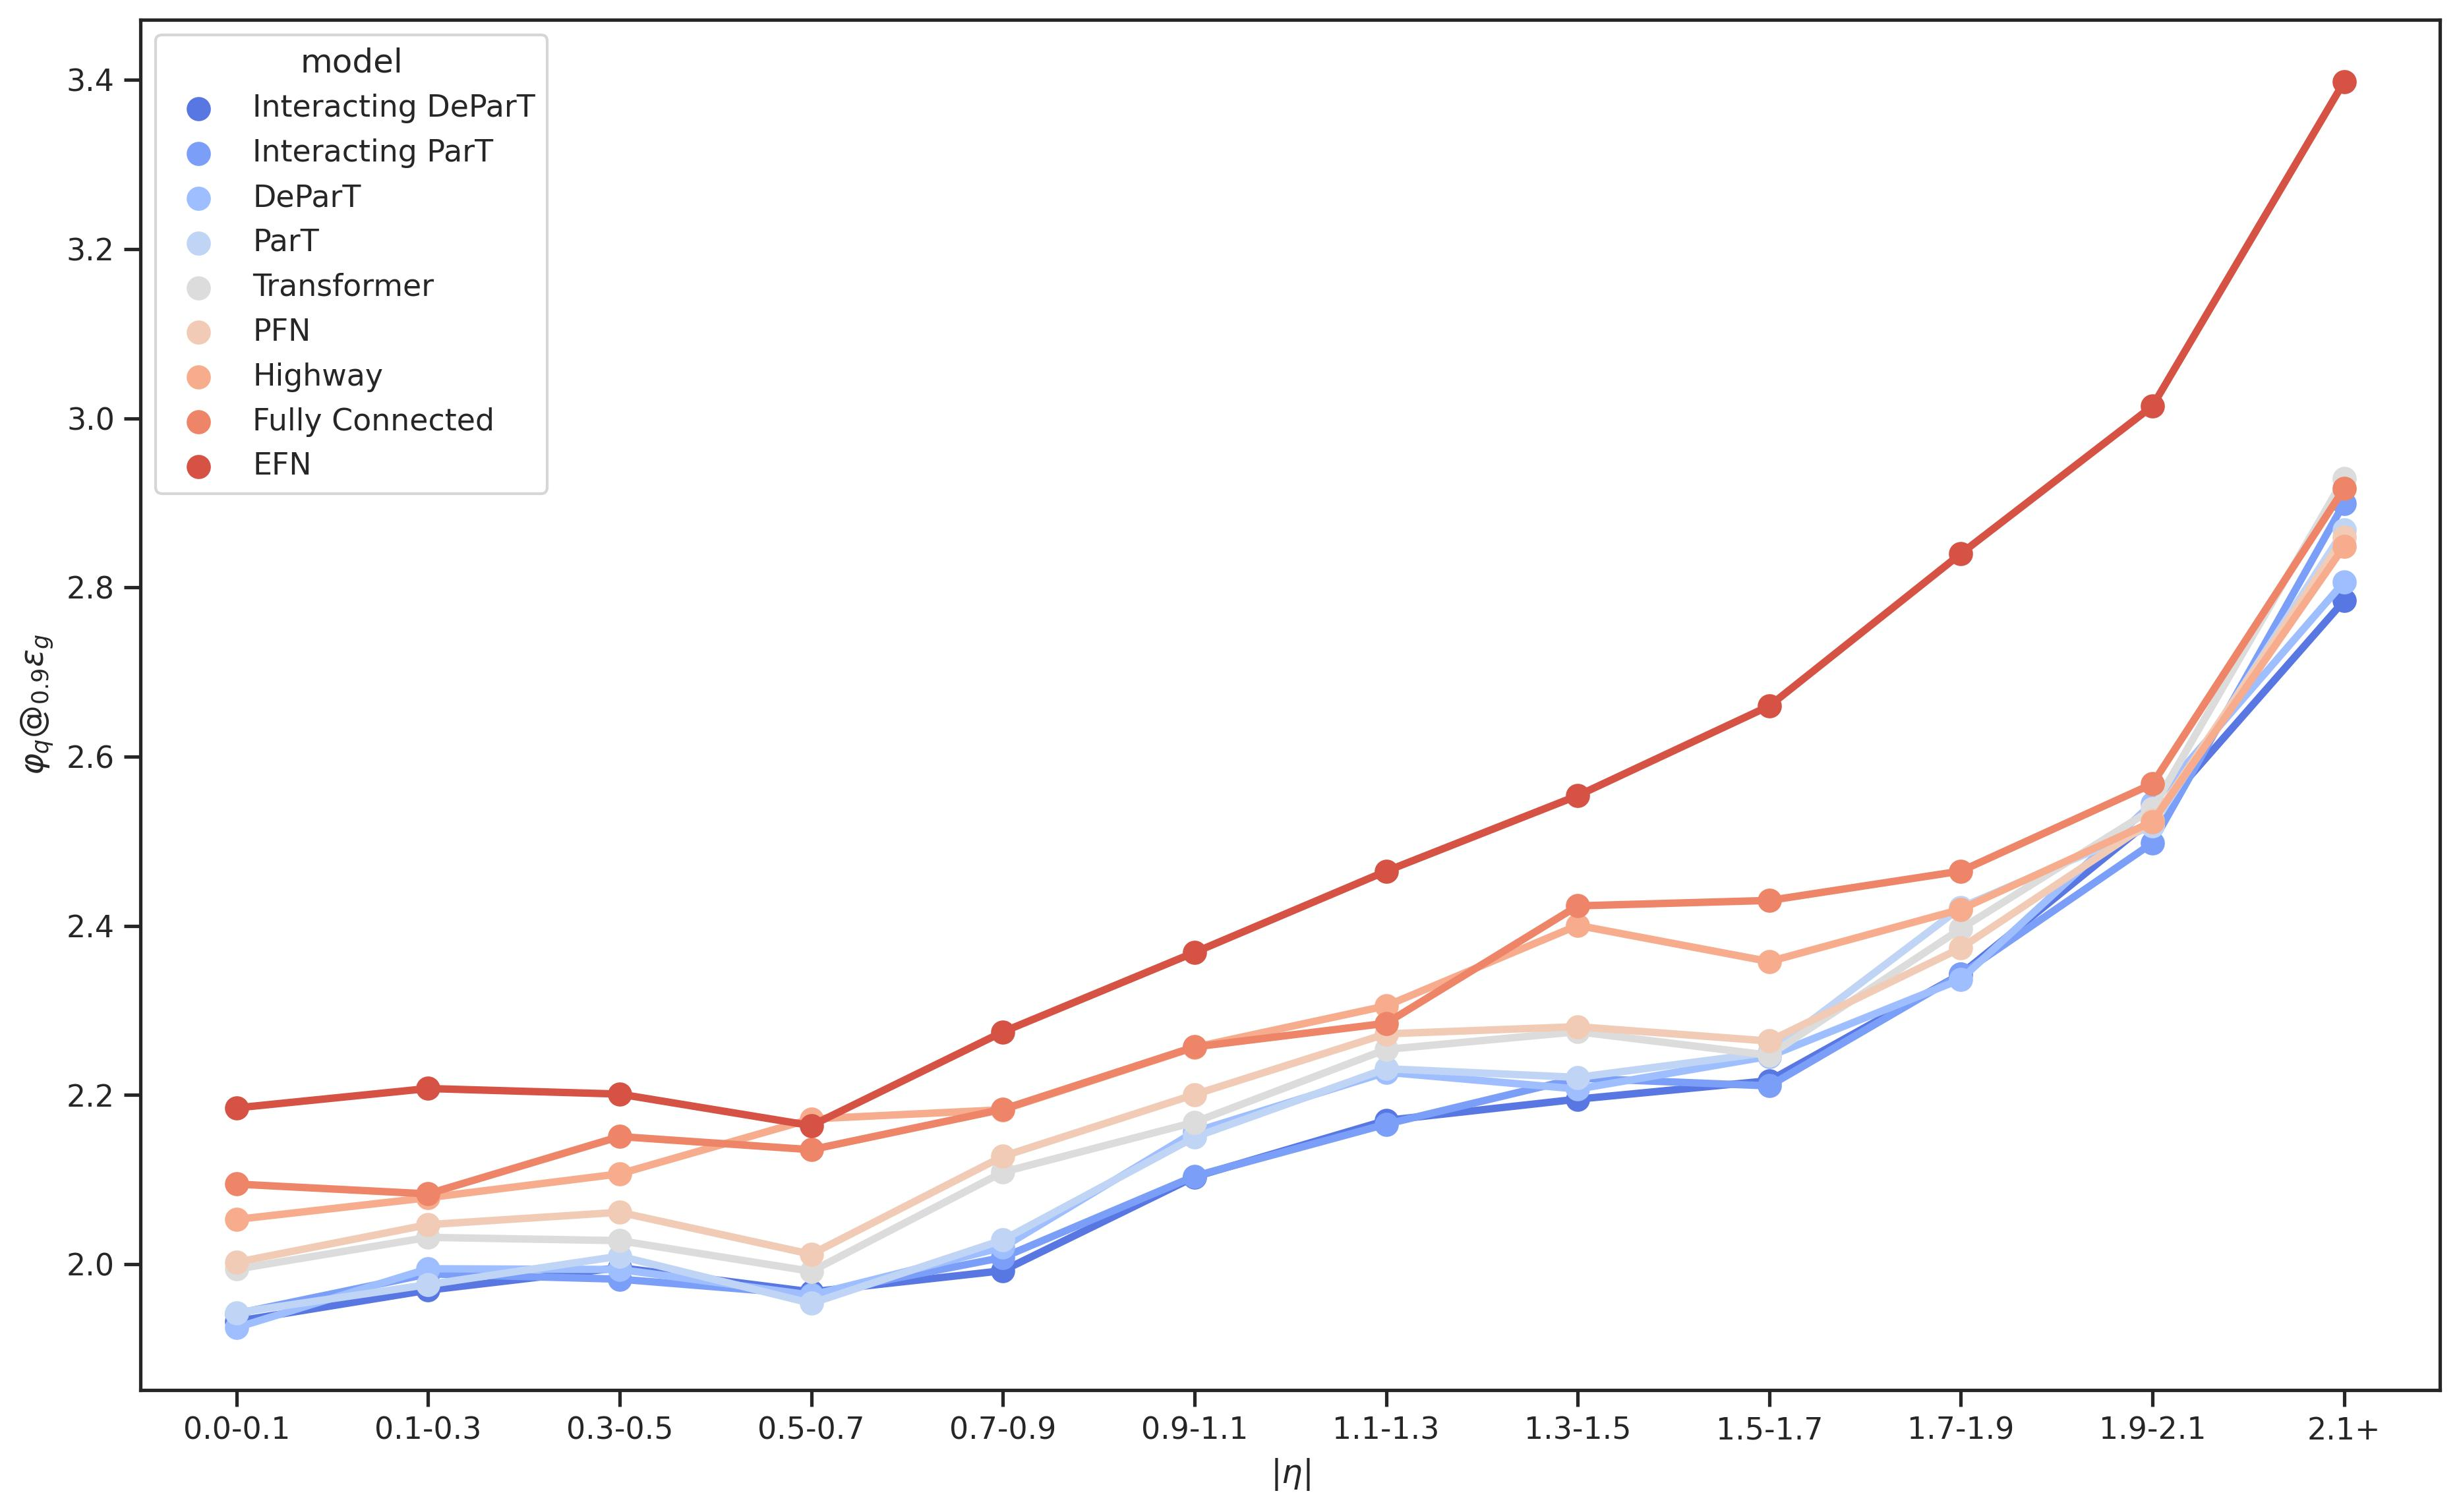
\includegraphics[width=0.95\linewidth]{src/plots/results/eta_dep/quark_rej_at_gluon_eff_0.9.jpg}
    \caption{Quark rejection at gluon efficiency of 0.9 as a function of pseudo-rapidity.}
    \label{fig:quark_rej_at_gluon_eff_0.9_eta}
\end{figure}

\begin{figure}[htb]
    \centering
    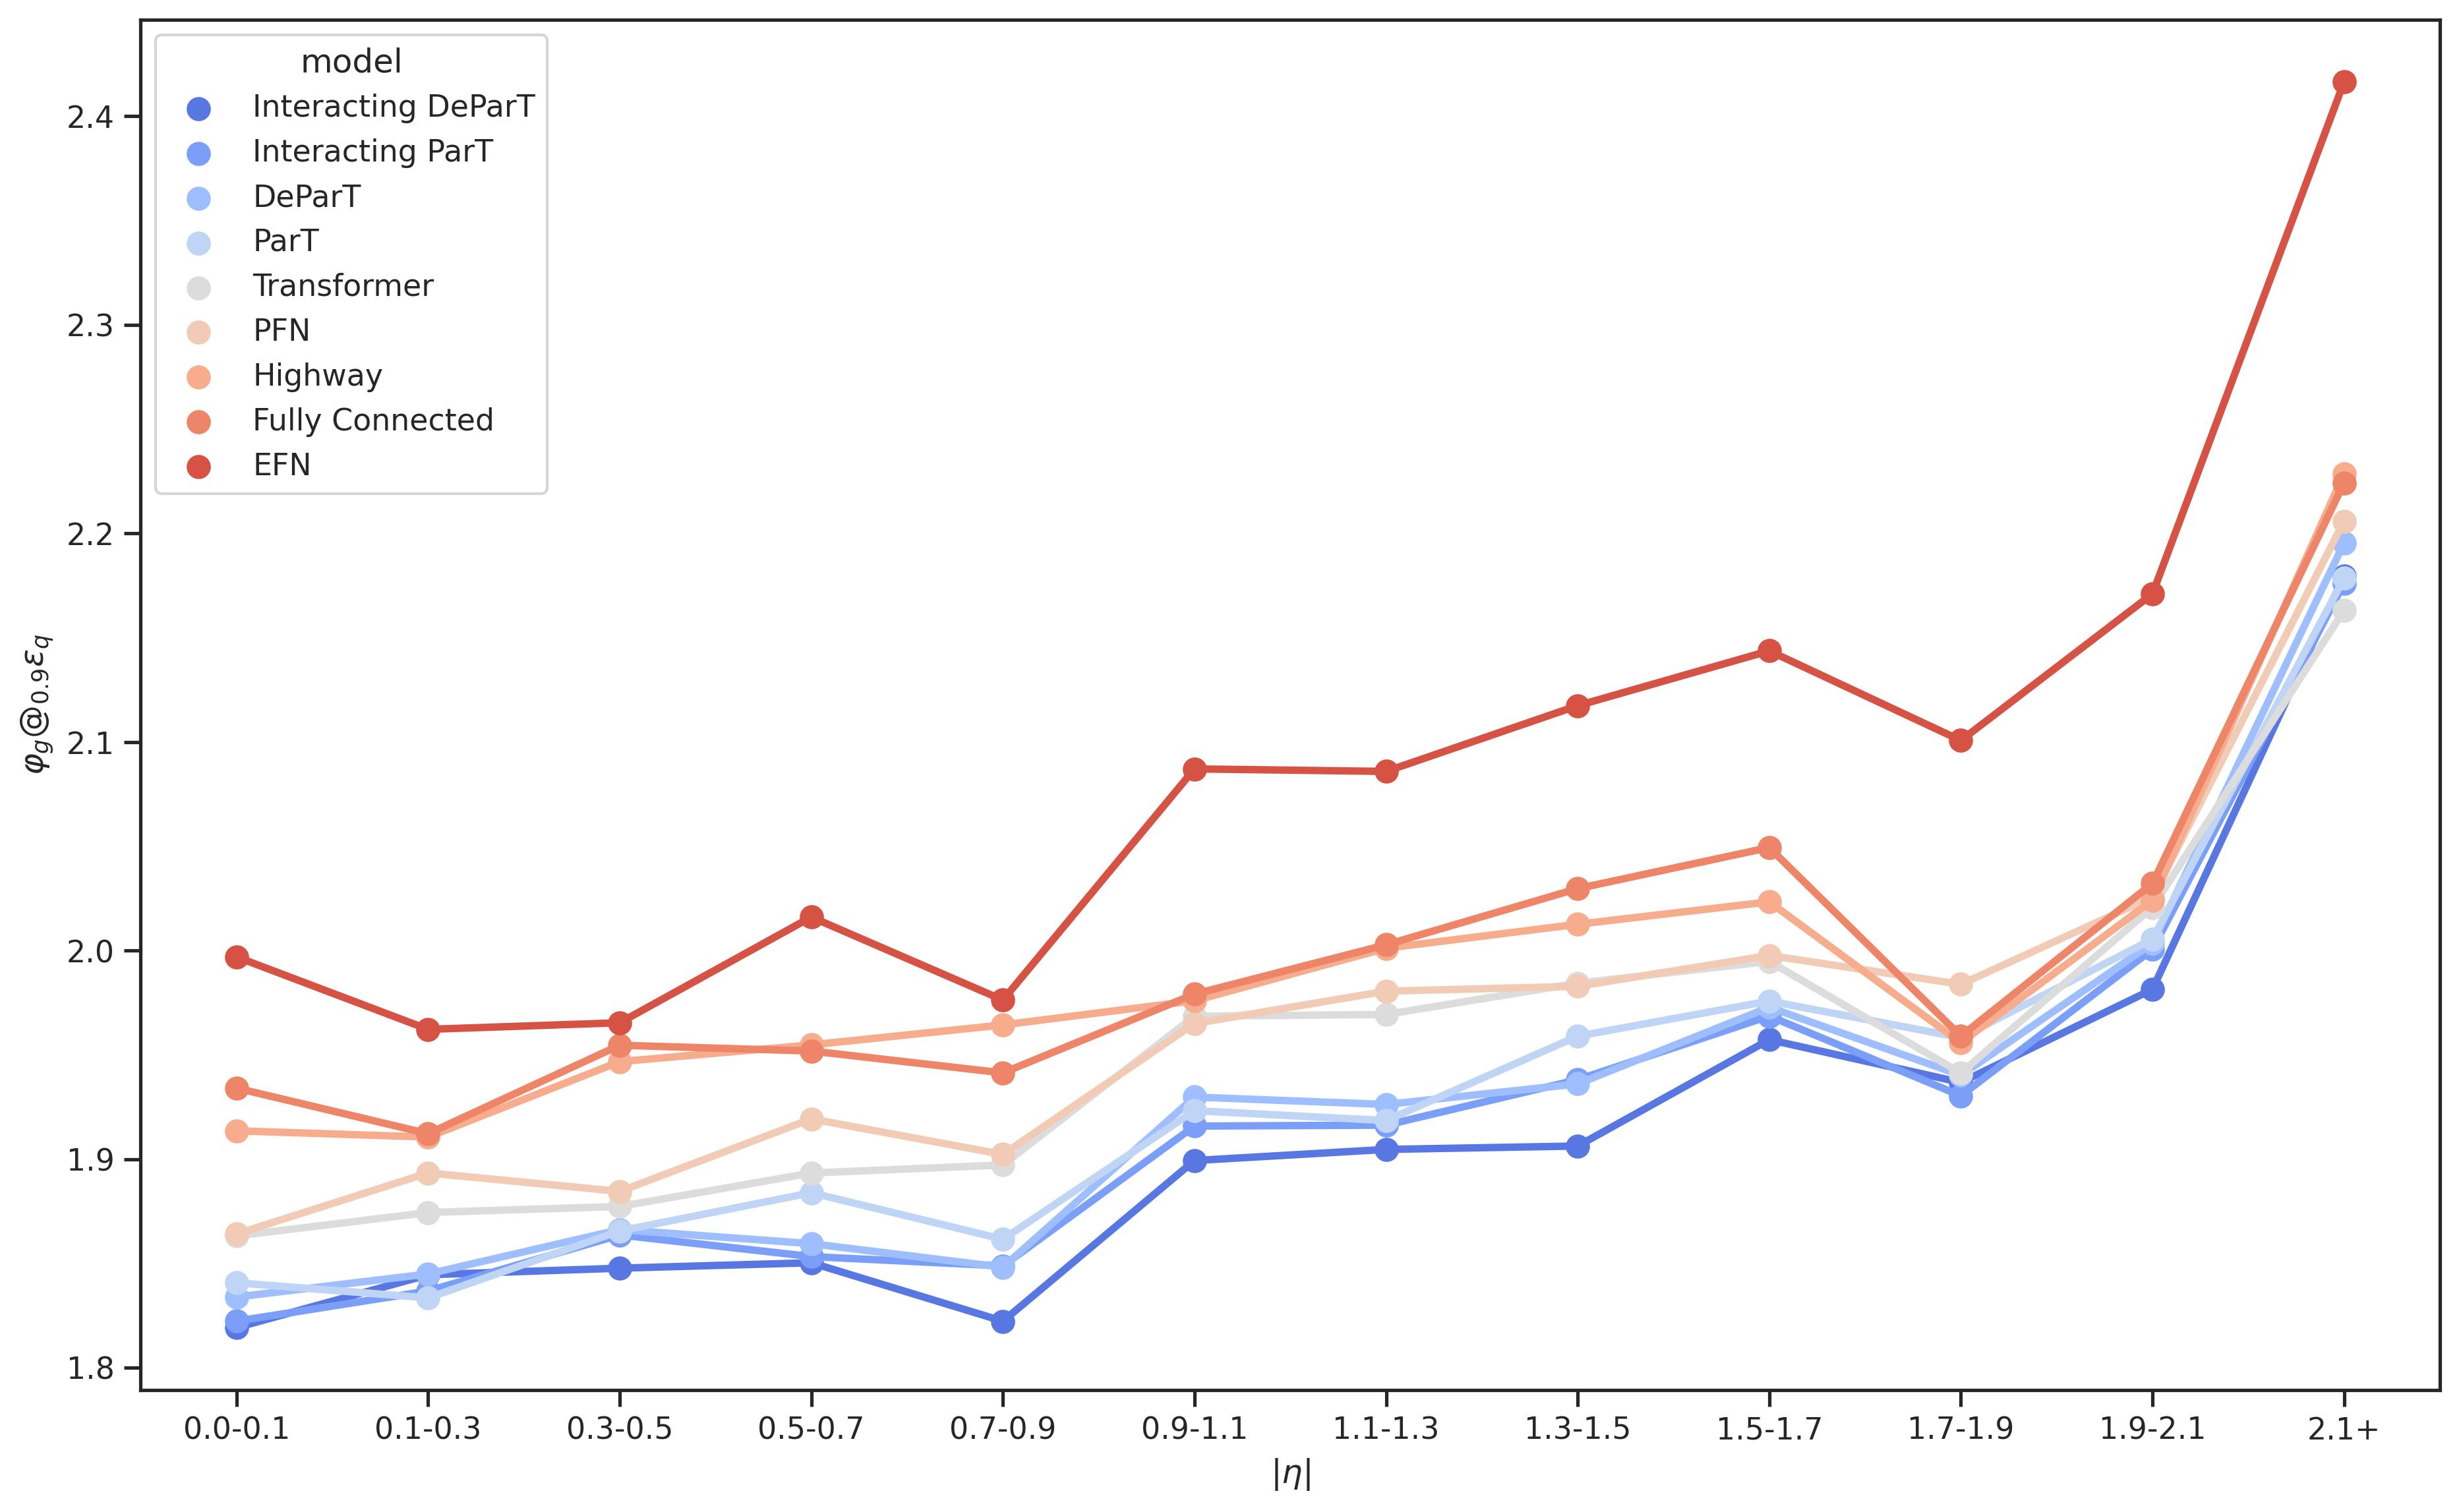
\includegraphics[width=0.95\linewidth]{src/plots/results/eta_dep/gluon_rej_at_quark_eff_0.9.jpg}
    \caption{Gluon rejection at quark efficiency of 0.9 as a function of pseudo-rapidity.}
    \label{fig:gluon_rej_at_quark_eff_0.9_eta}
\end{figure}

\begin{figure}[htb]
    \centering
    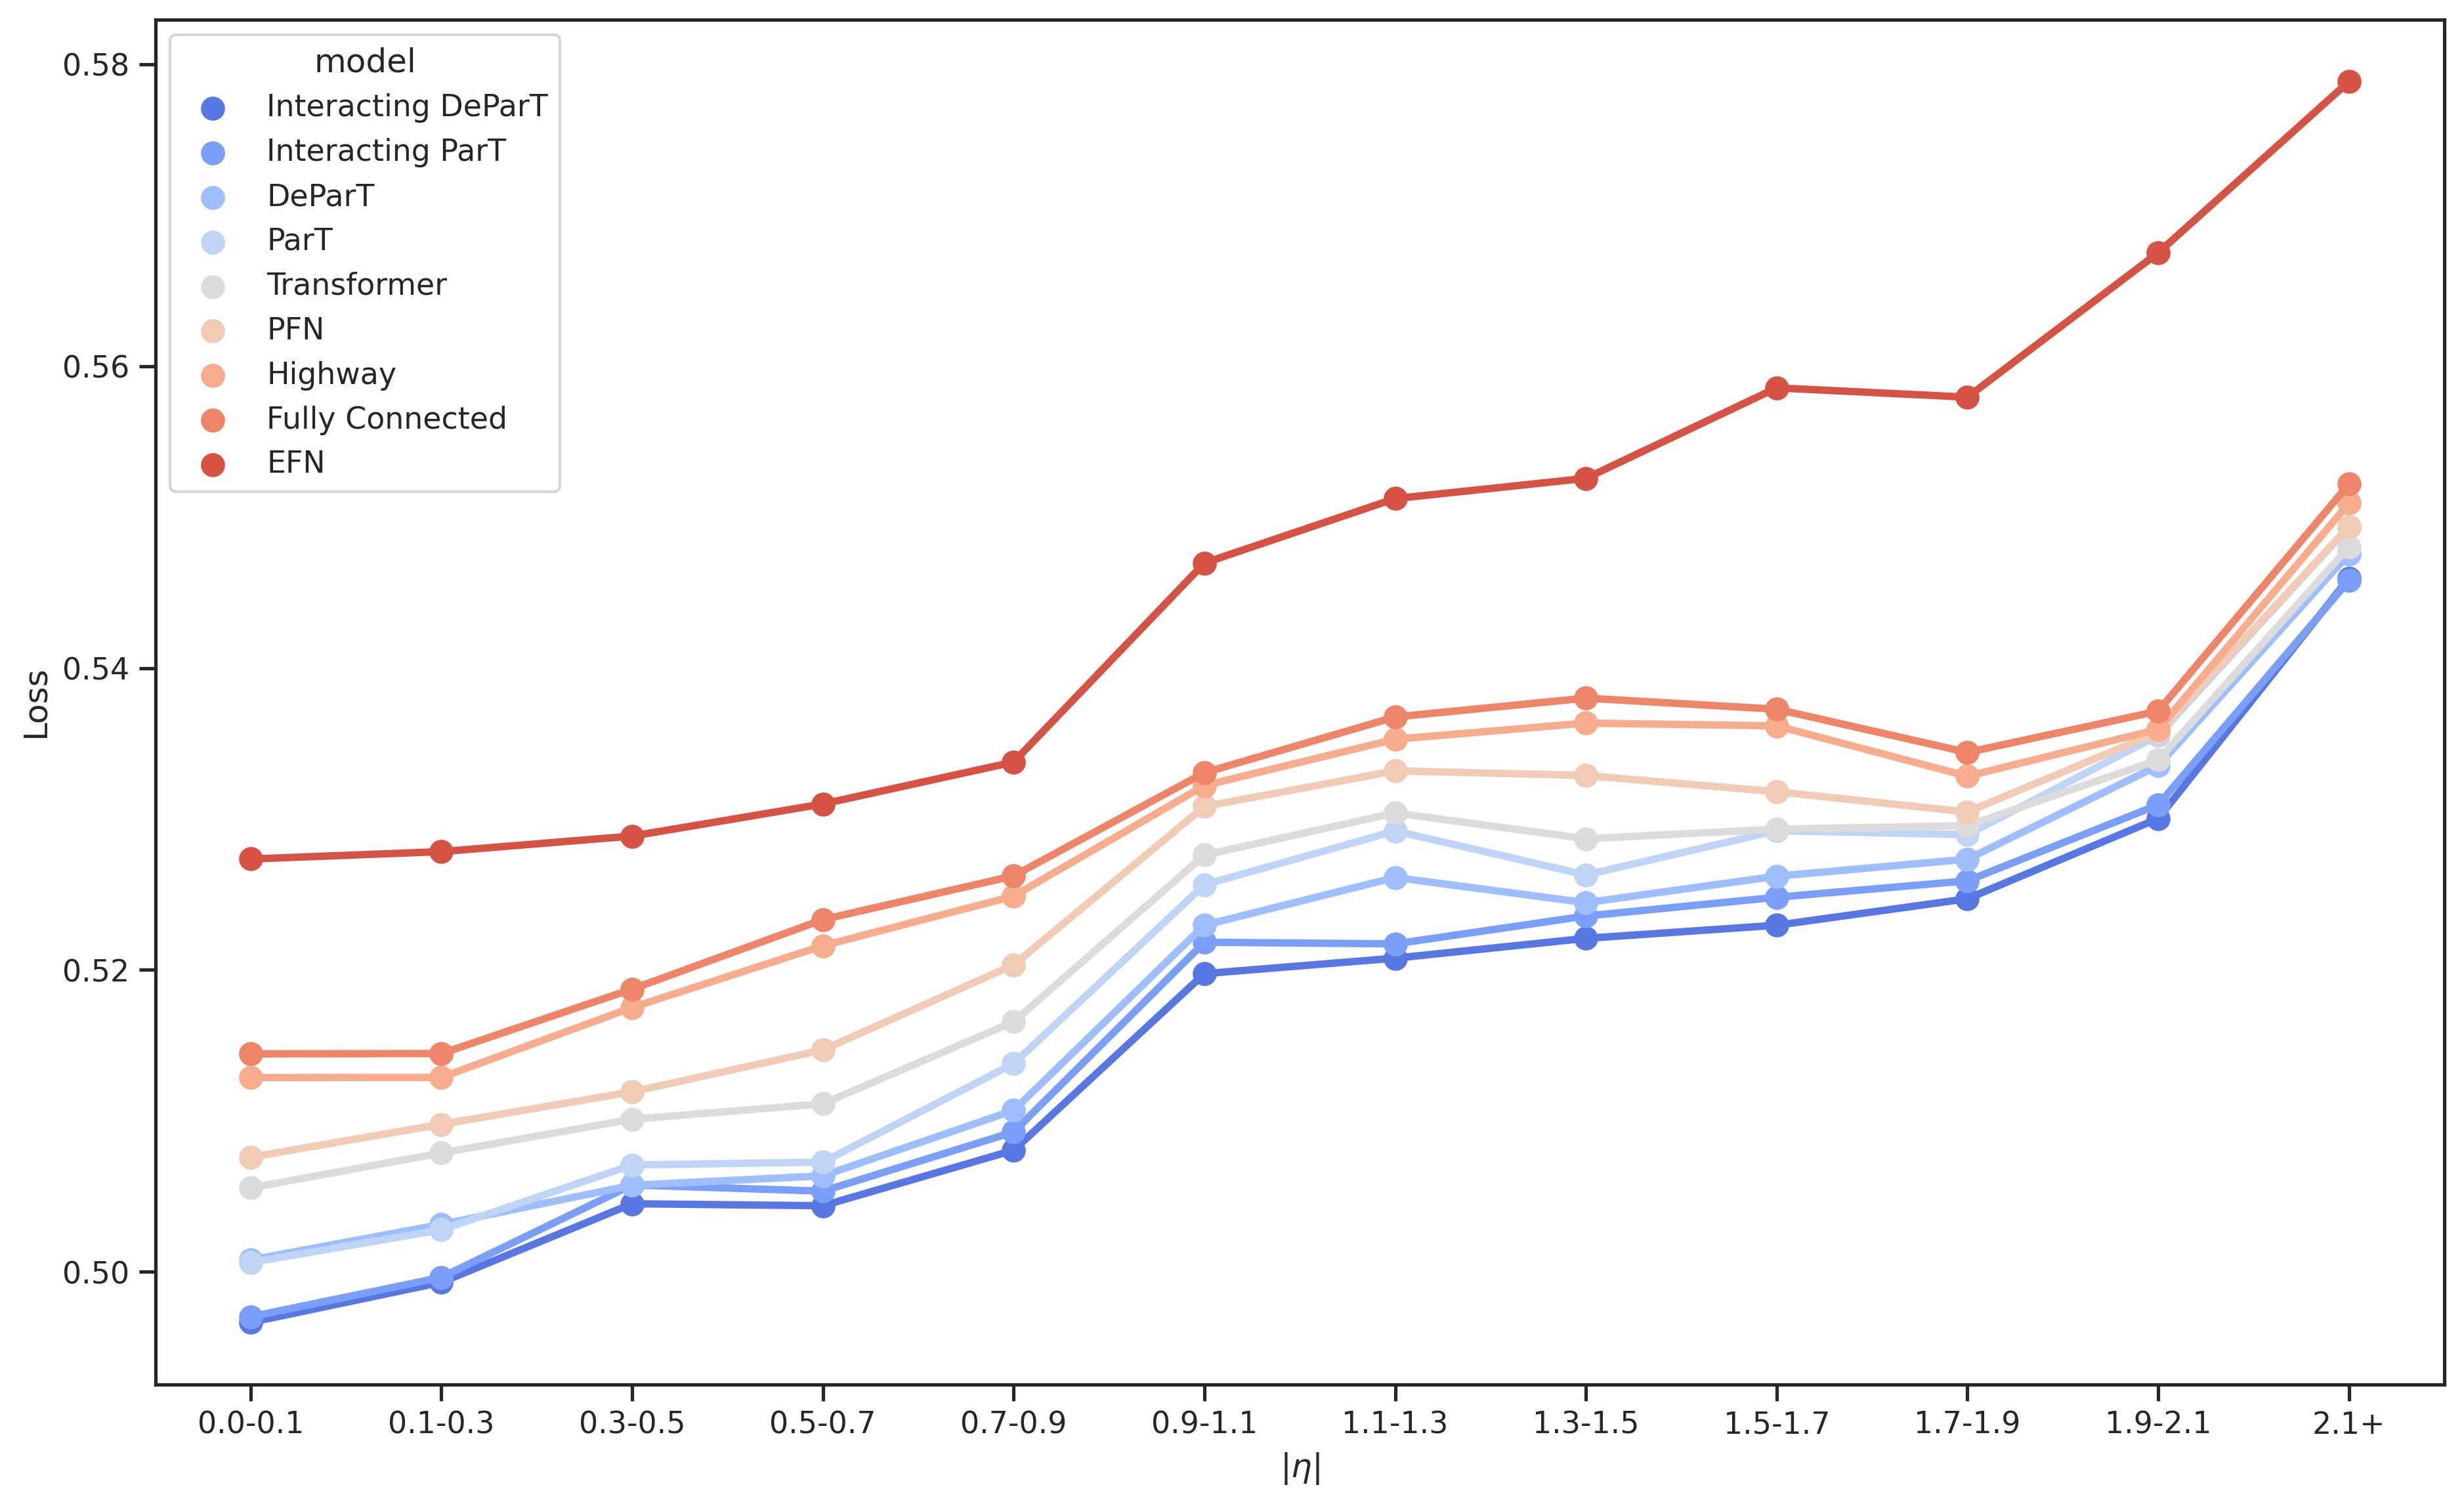
\includegraphics[width=0.95\linewidth]{src/plots/results/eta_dep/loss.jpg}
    \caption{Loss as a function of pseudo-rapidity.}
    \label{fig:loss_eta}
\end{figure}

\FloatBarrier

\section{Pileup Dependence}
\label{sec:app_pileup_dep}

\begin{figure}[htb]
    \centering
    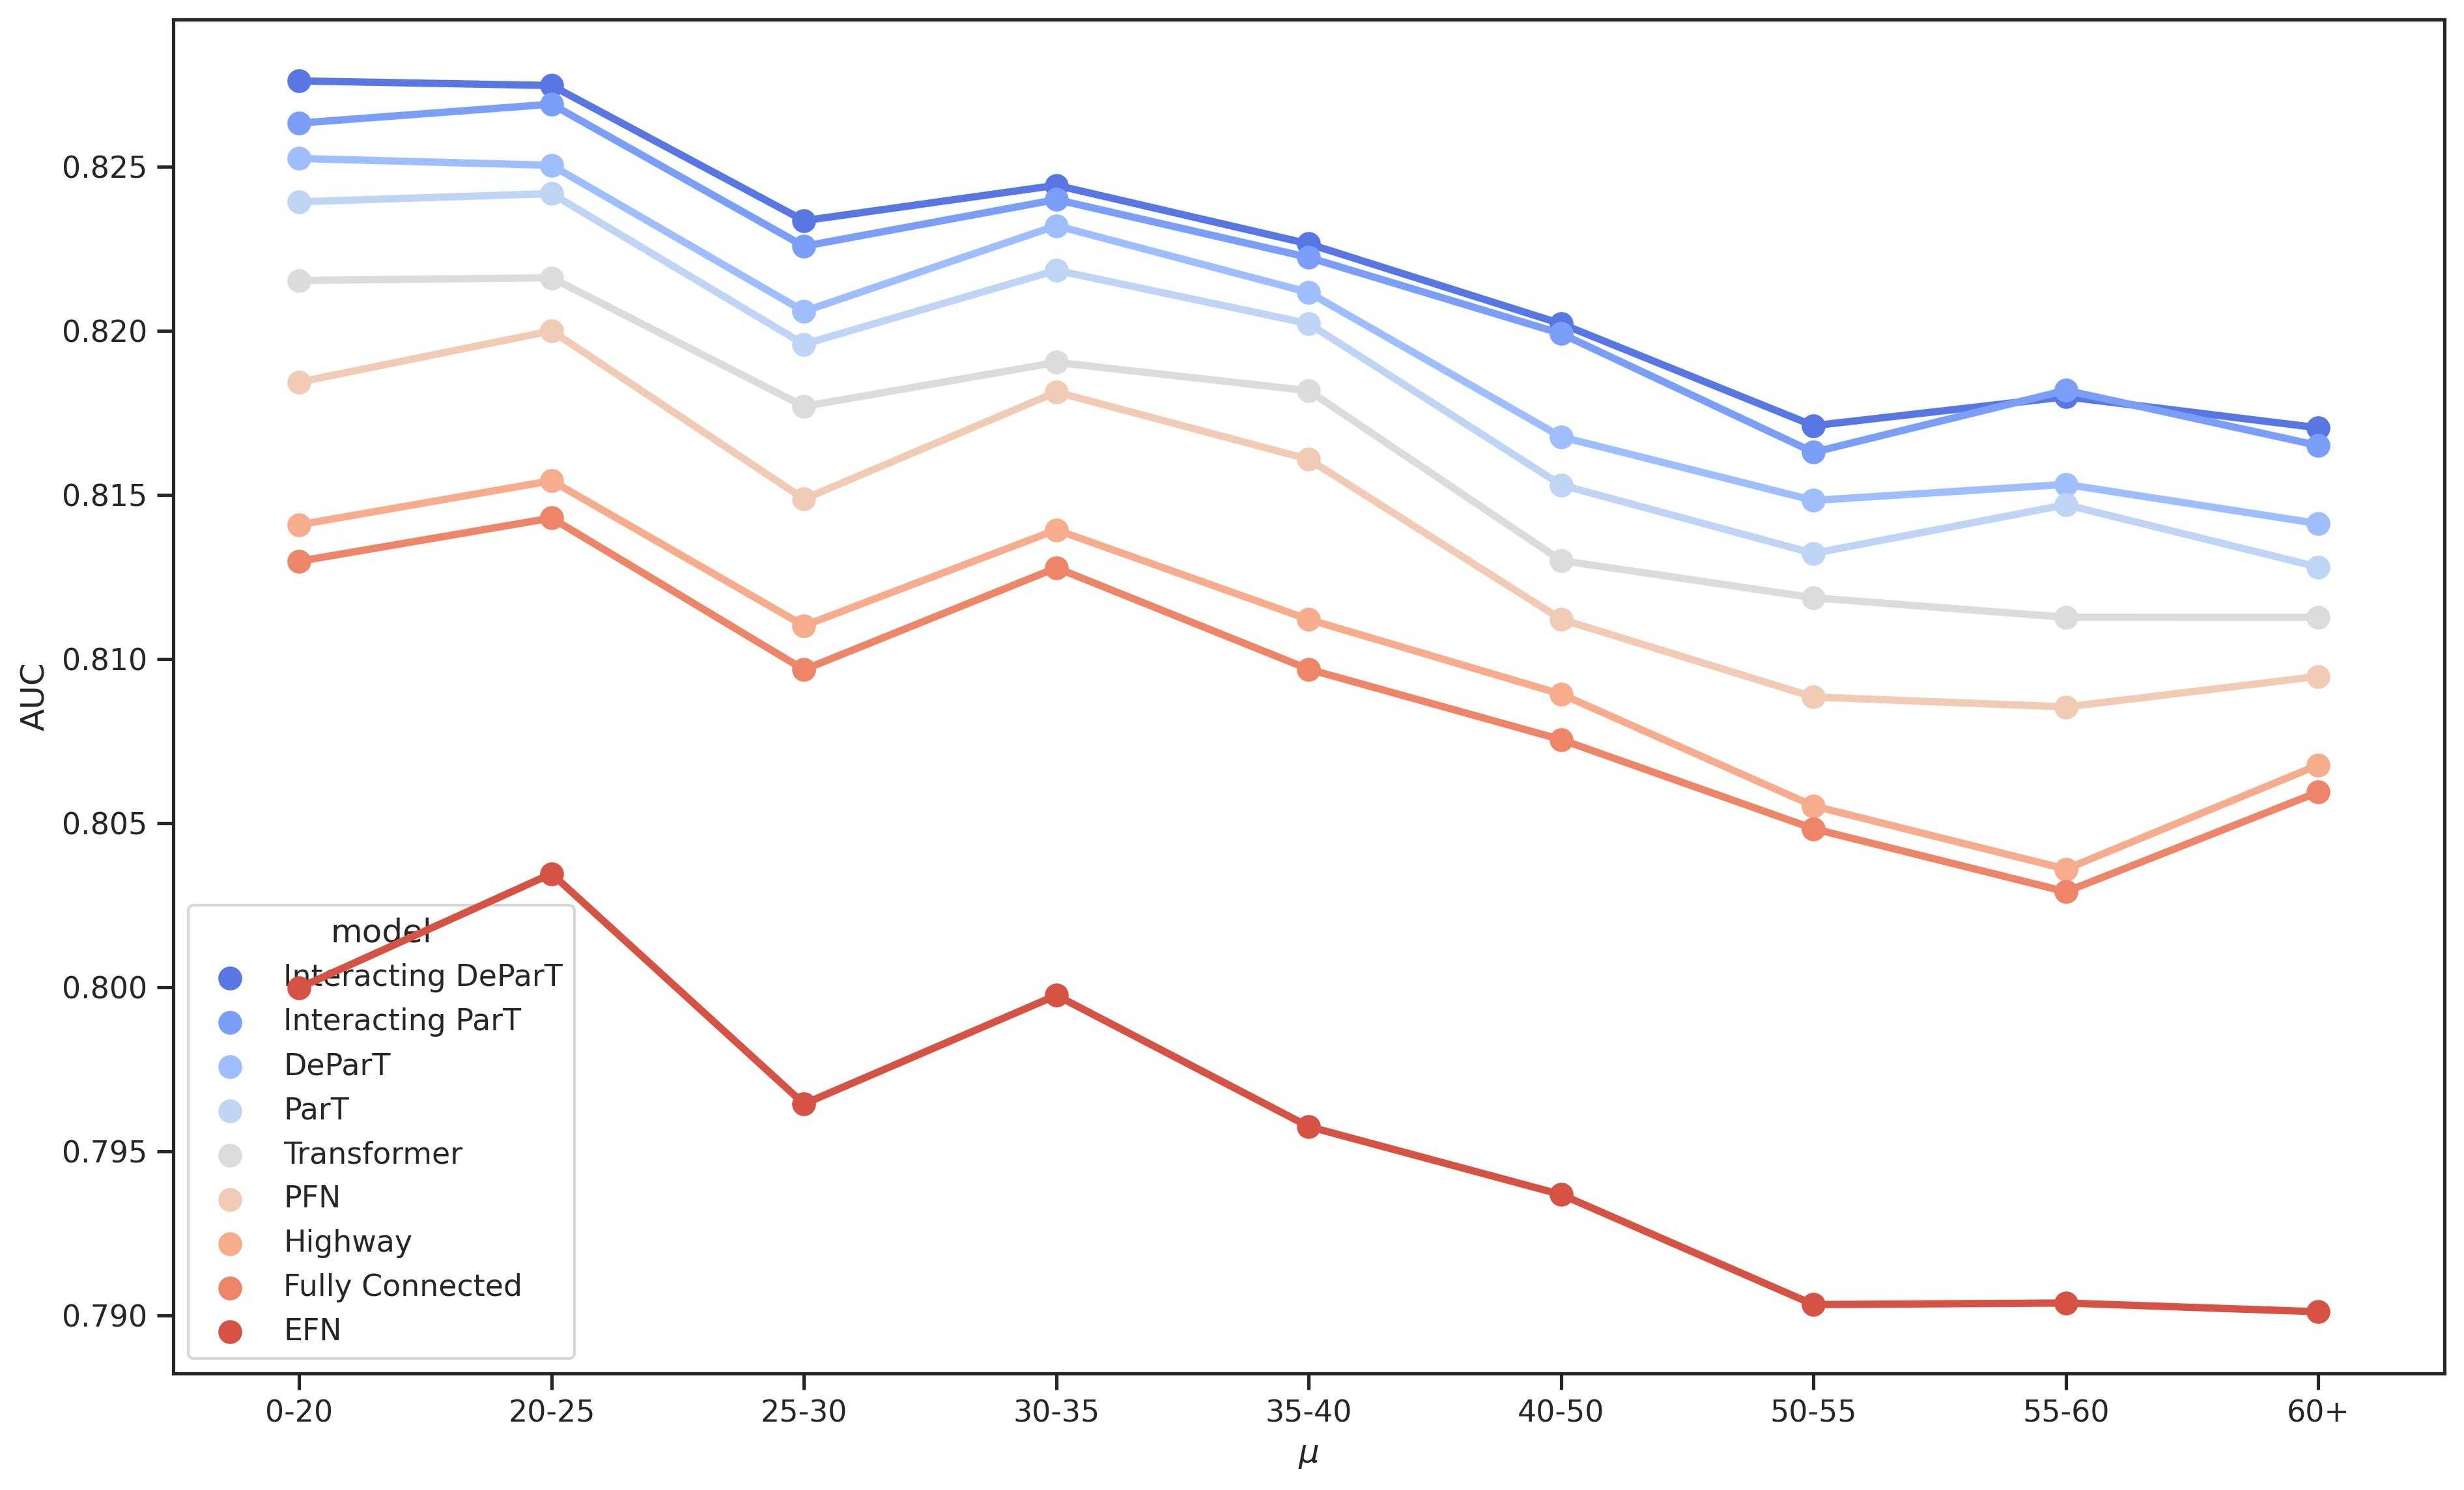
\includegraphics[width=0.95\linewidth]{src/plots/results/mu_dep/auc.jpg}
    \caption{AUC as a function of pileup.}
    \label{fig:auc_pileup}
\end{figure}

\begin{figure}[htb]
    \centering
    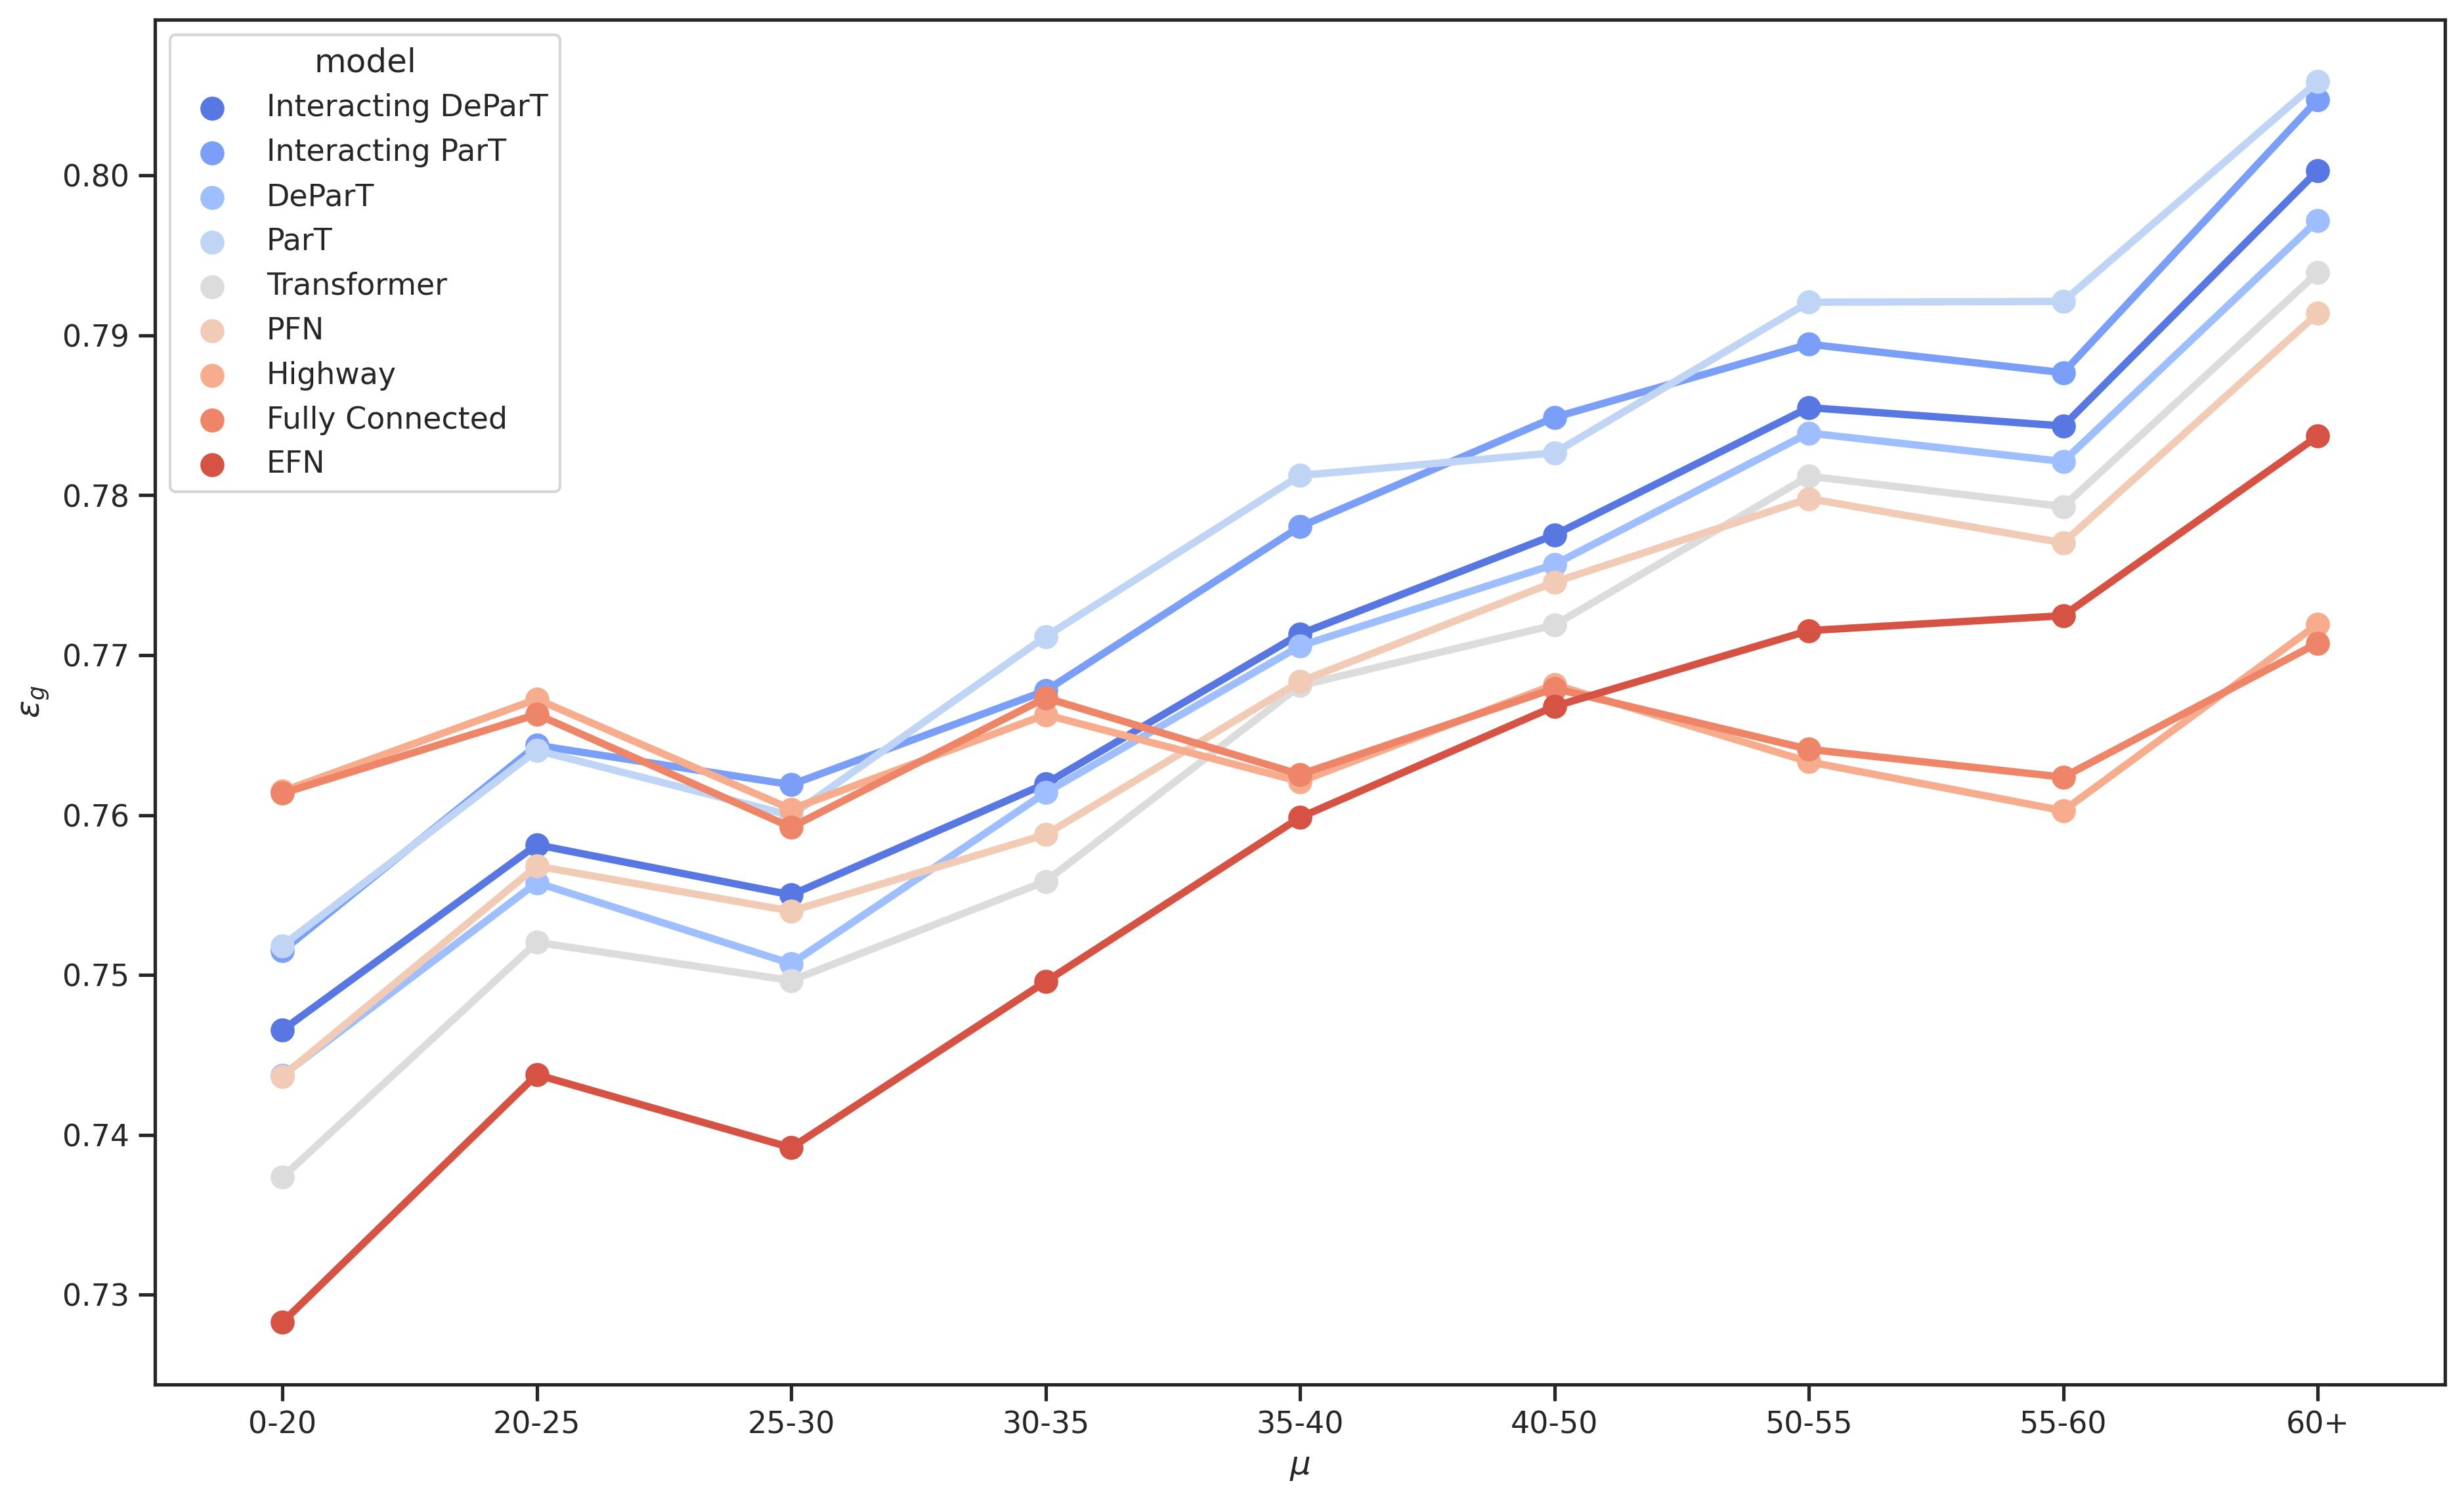
\includegraphics[width=0.95\linewidth]{src/plots/results/mu_dep/gluon_efficiency.jpg}
    \caption{Gluon efficiency as a function of pileup.}
    \label{fig:gluon_eff_pileup}
\end{figure}

\begin{figure}[htb]
    \centering
    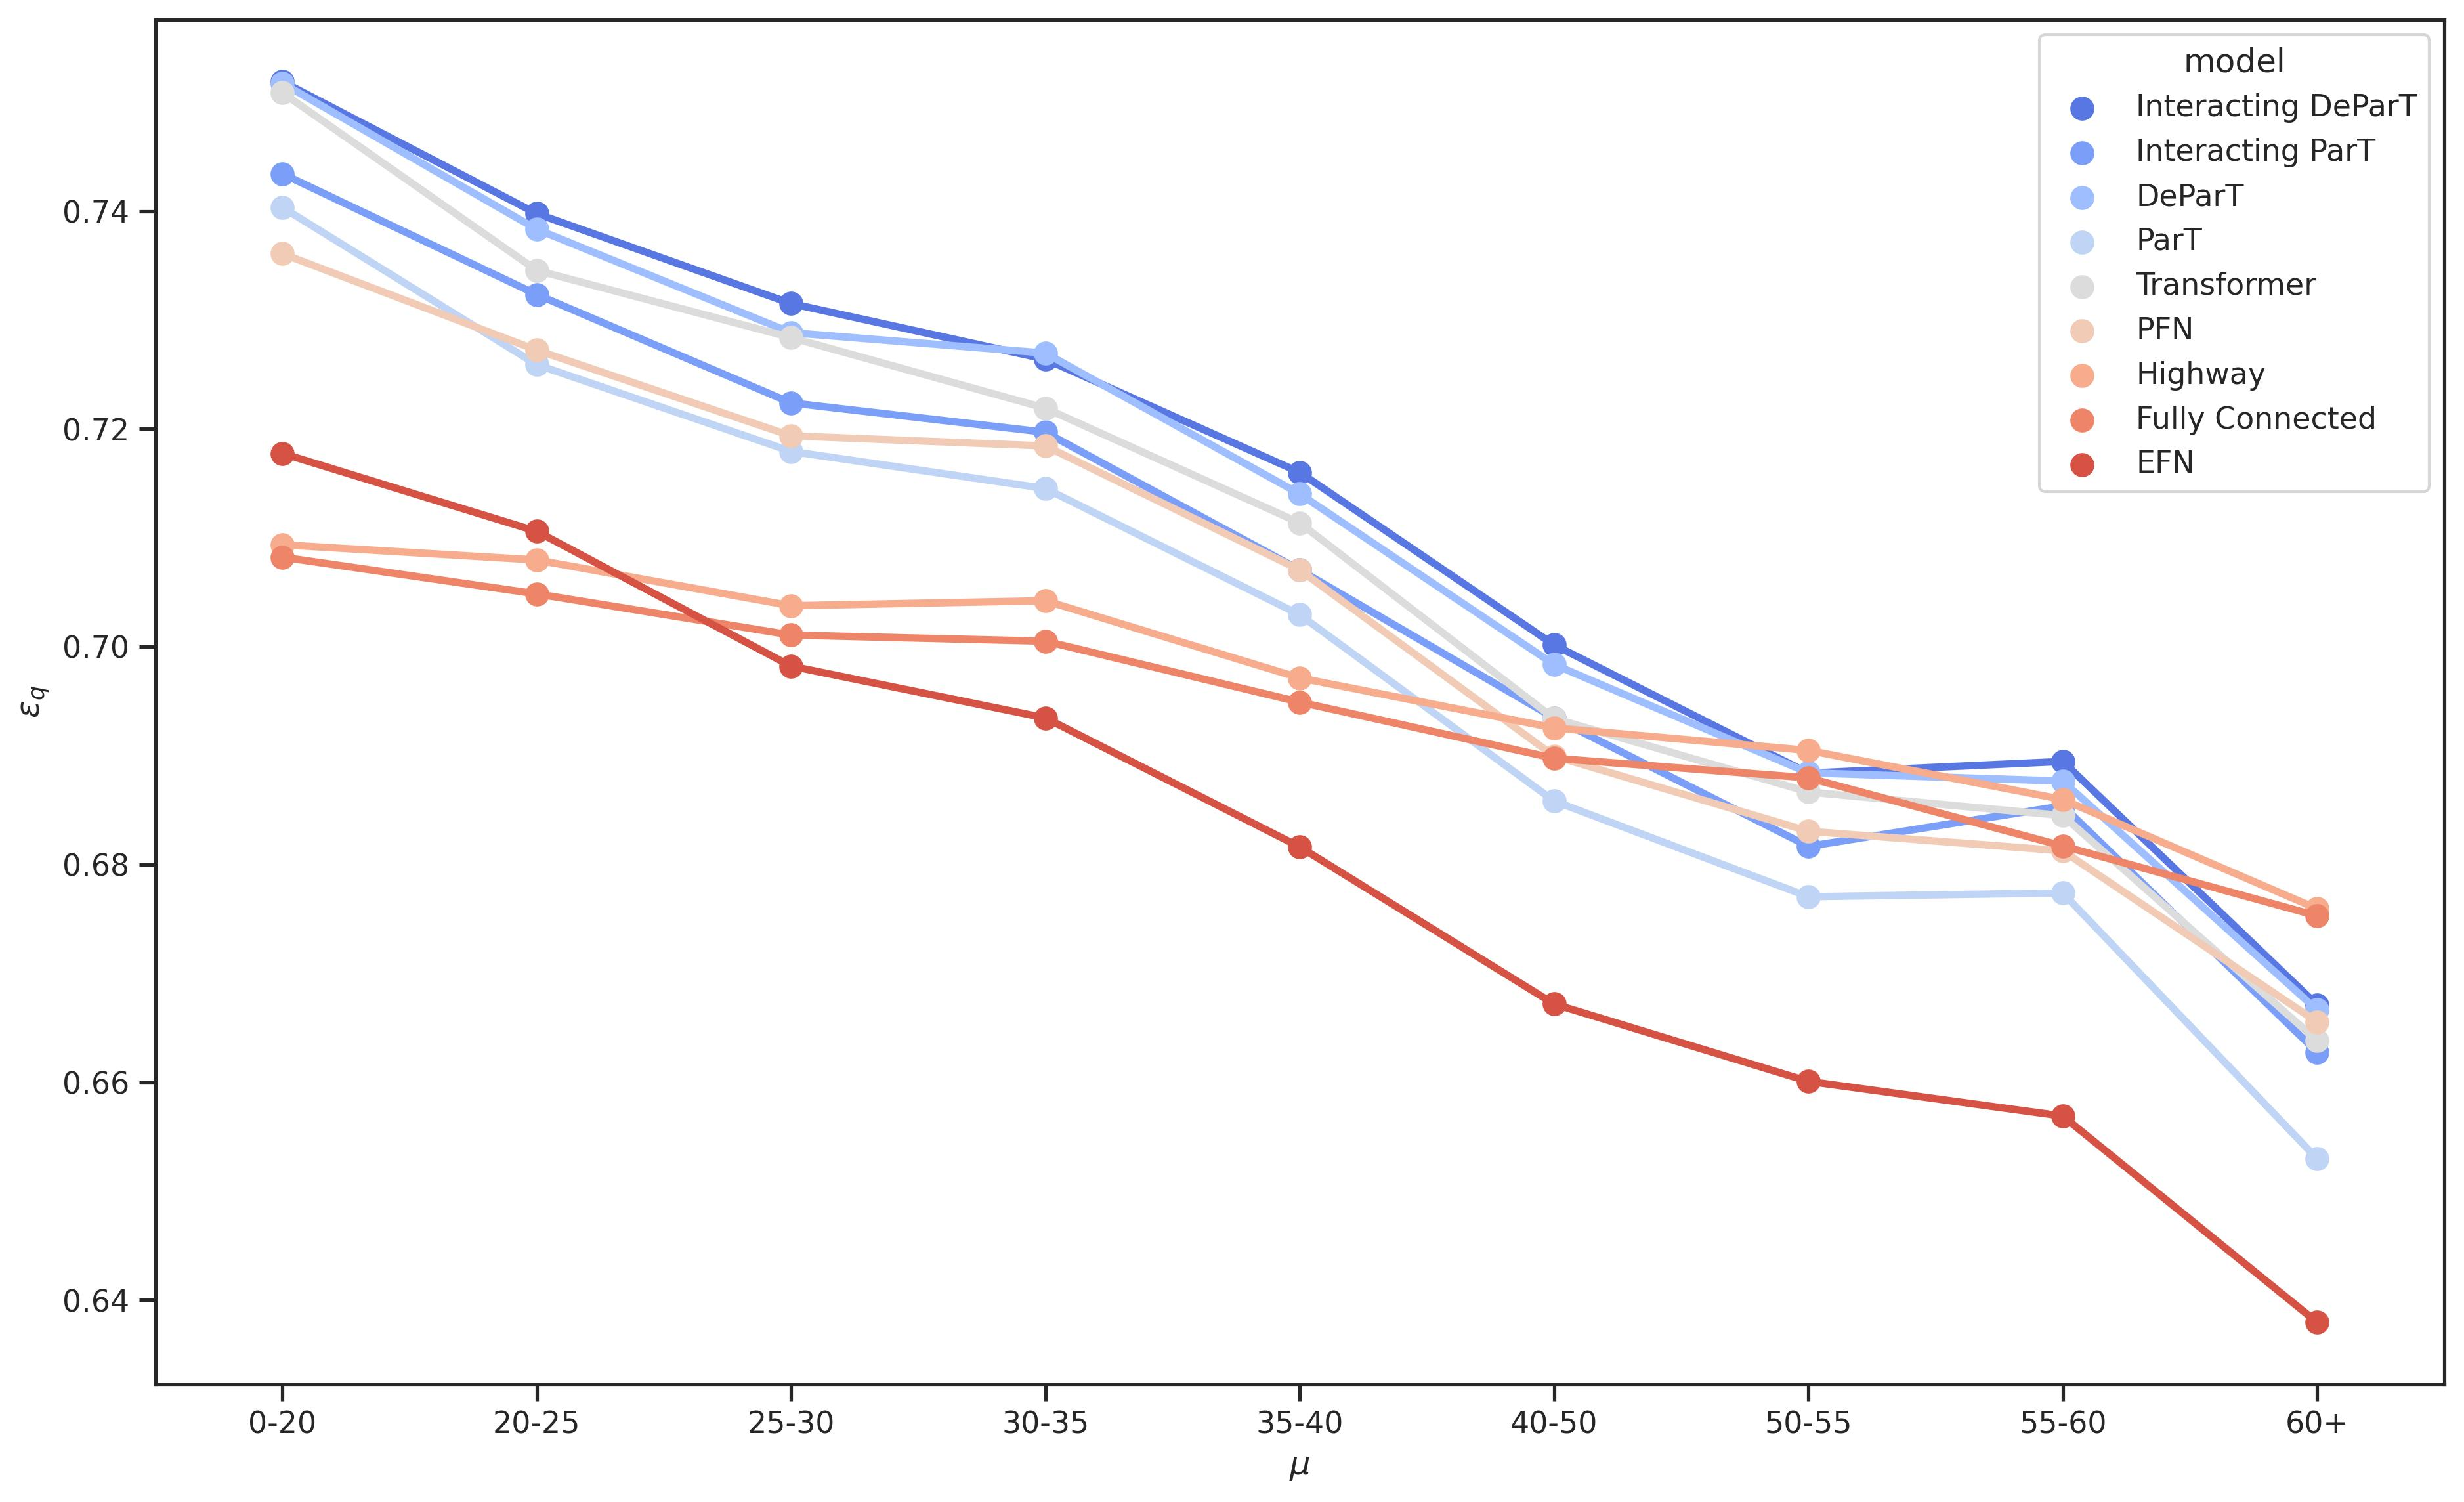
\includegraphics[width=0.95\linewidth]{src/plots/results/mu_dep/quark_efficiency.jpg}
    \caption{Quark efficiency as a function of pileup.}
    \label{fig:quark_eff_pileup}
\end{figure}

\begin{figure}[htb]
    \centering
    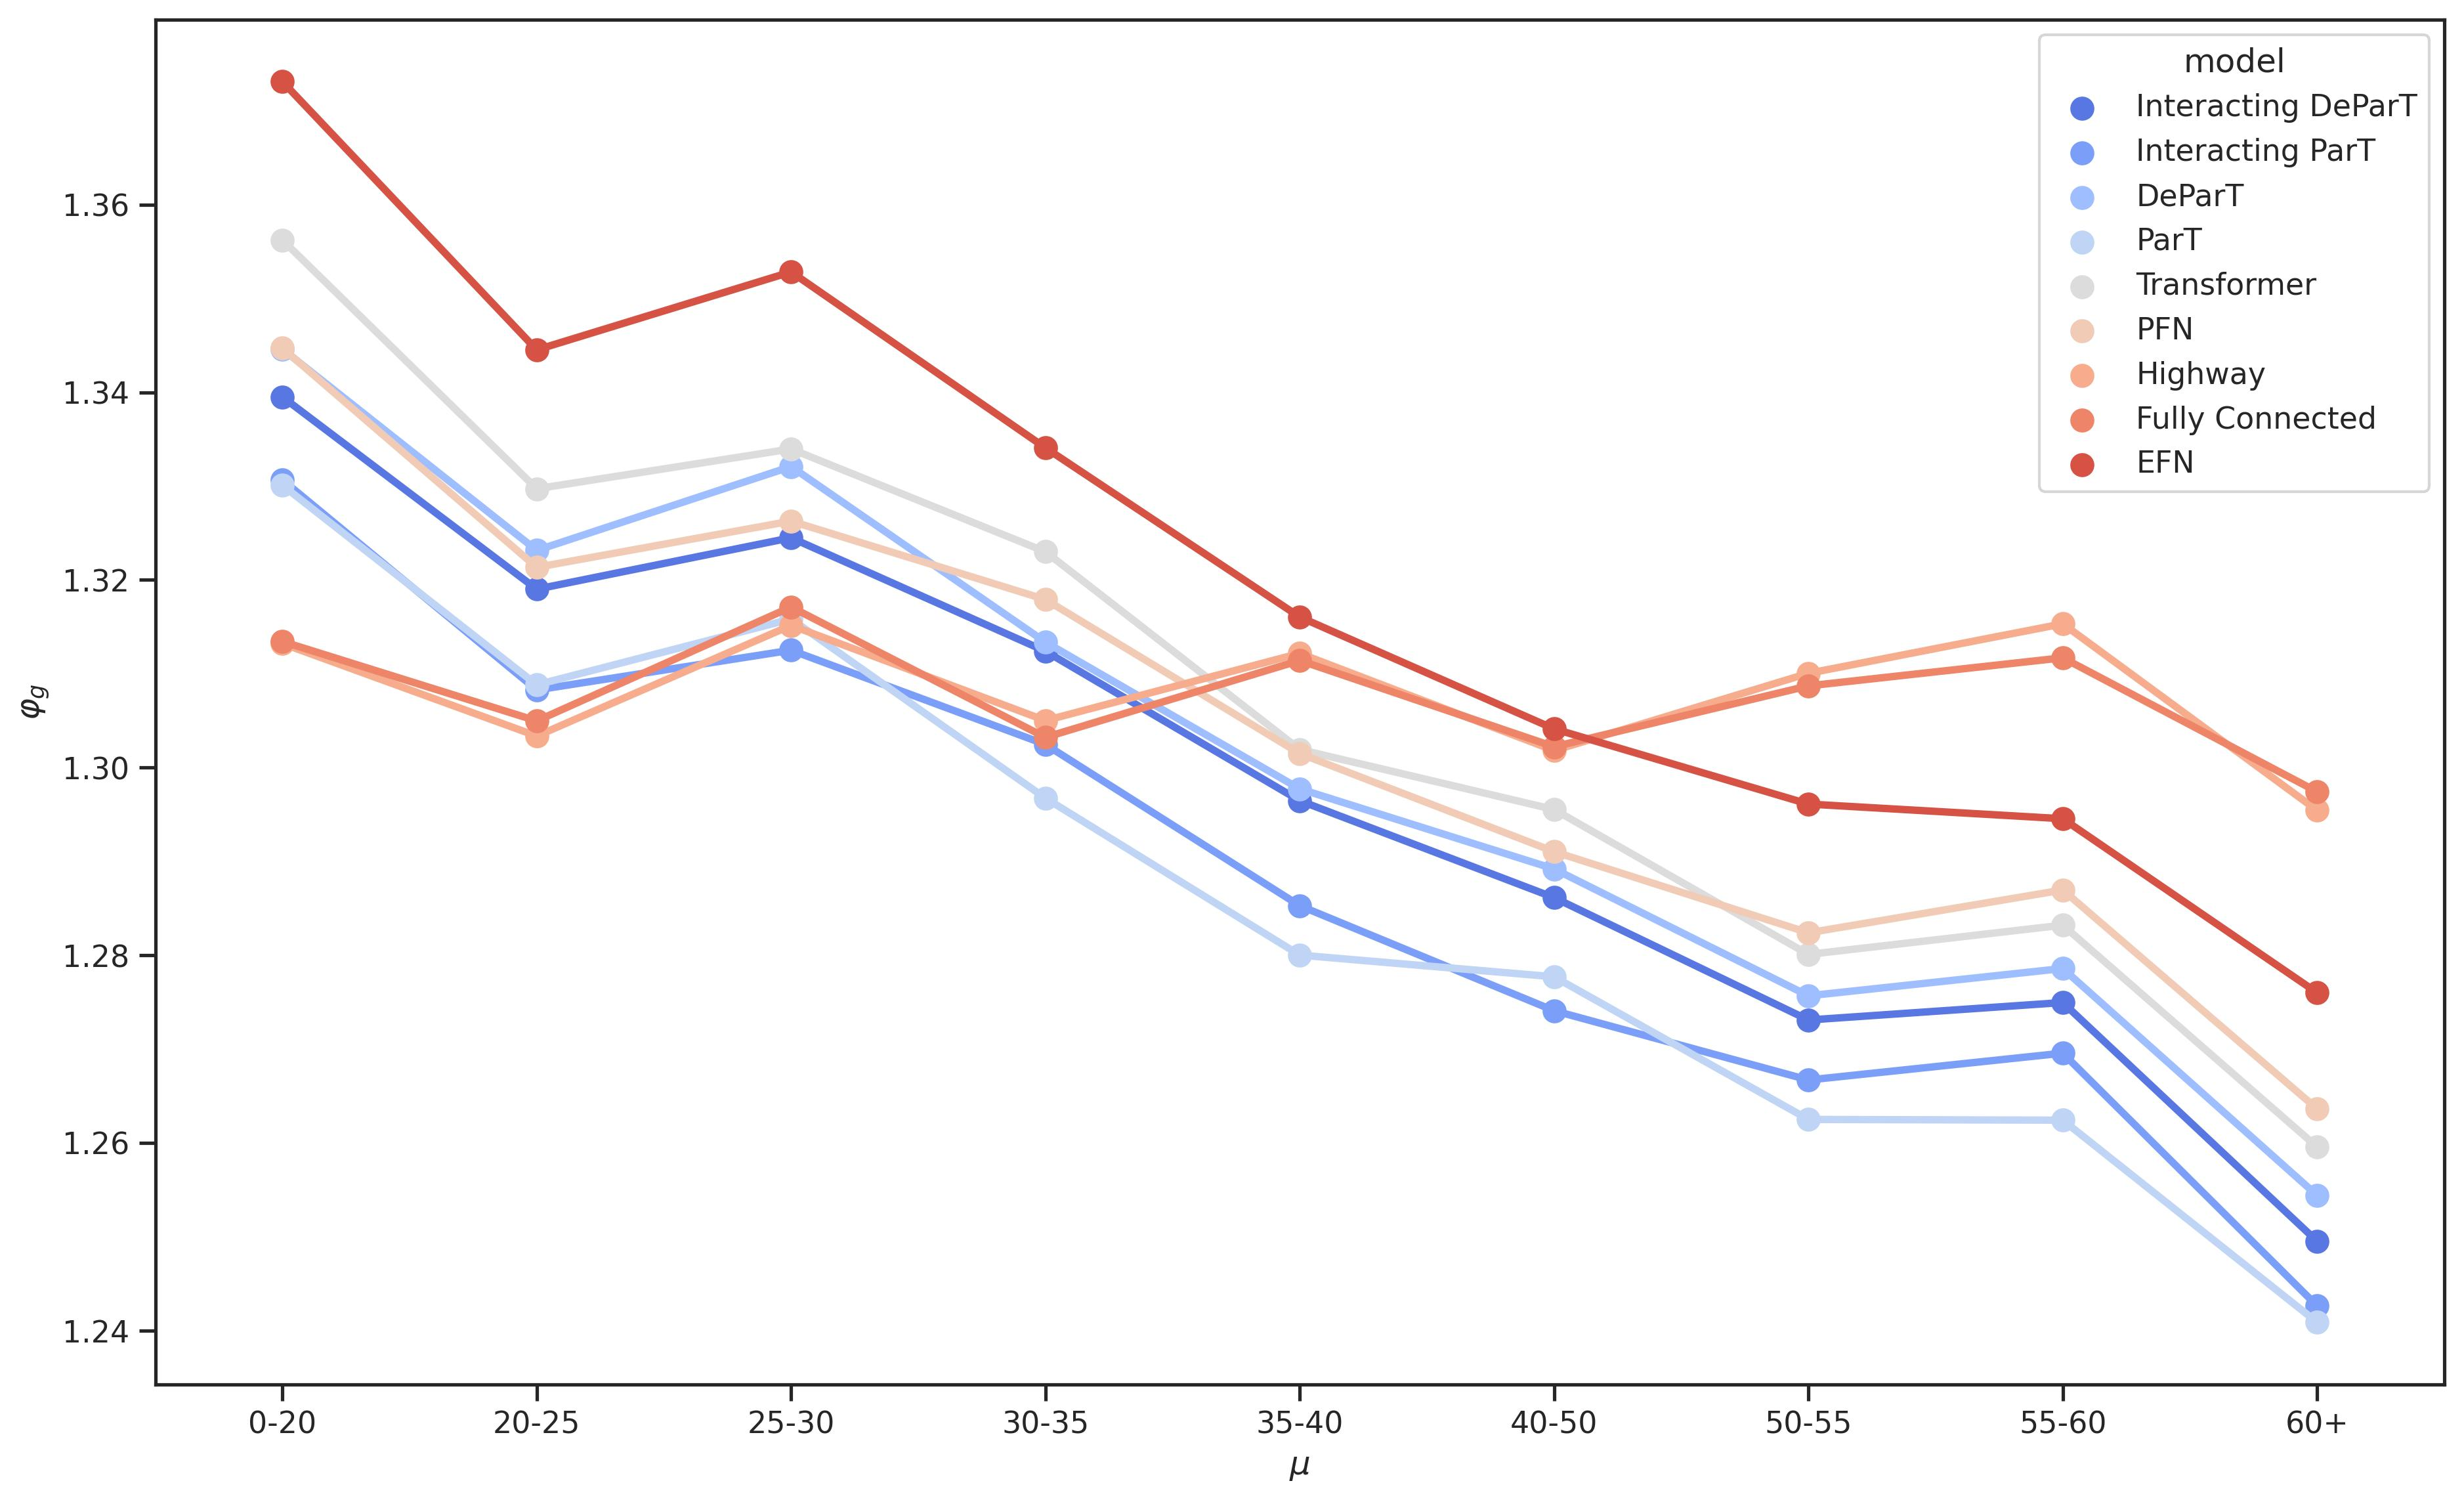
\includegraphics[width=0.95\linewidth]{src/plots/results/mu_dep/gluon_rejection.jpg}
    \caption{Gluon rejection as a function of pileup.}
    \label{fig:gluon_rej_pileup}
\end{figure}

\begin{figure}[htb]
    \centering
    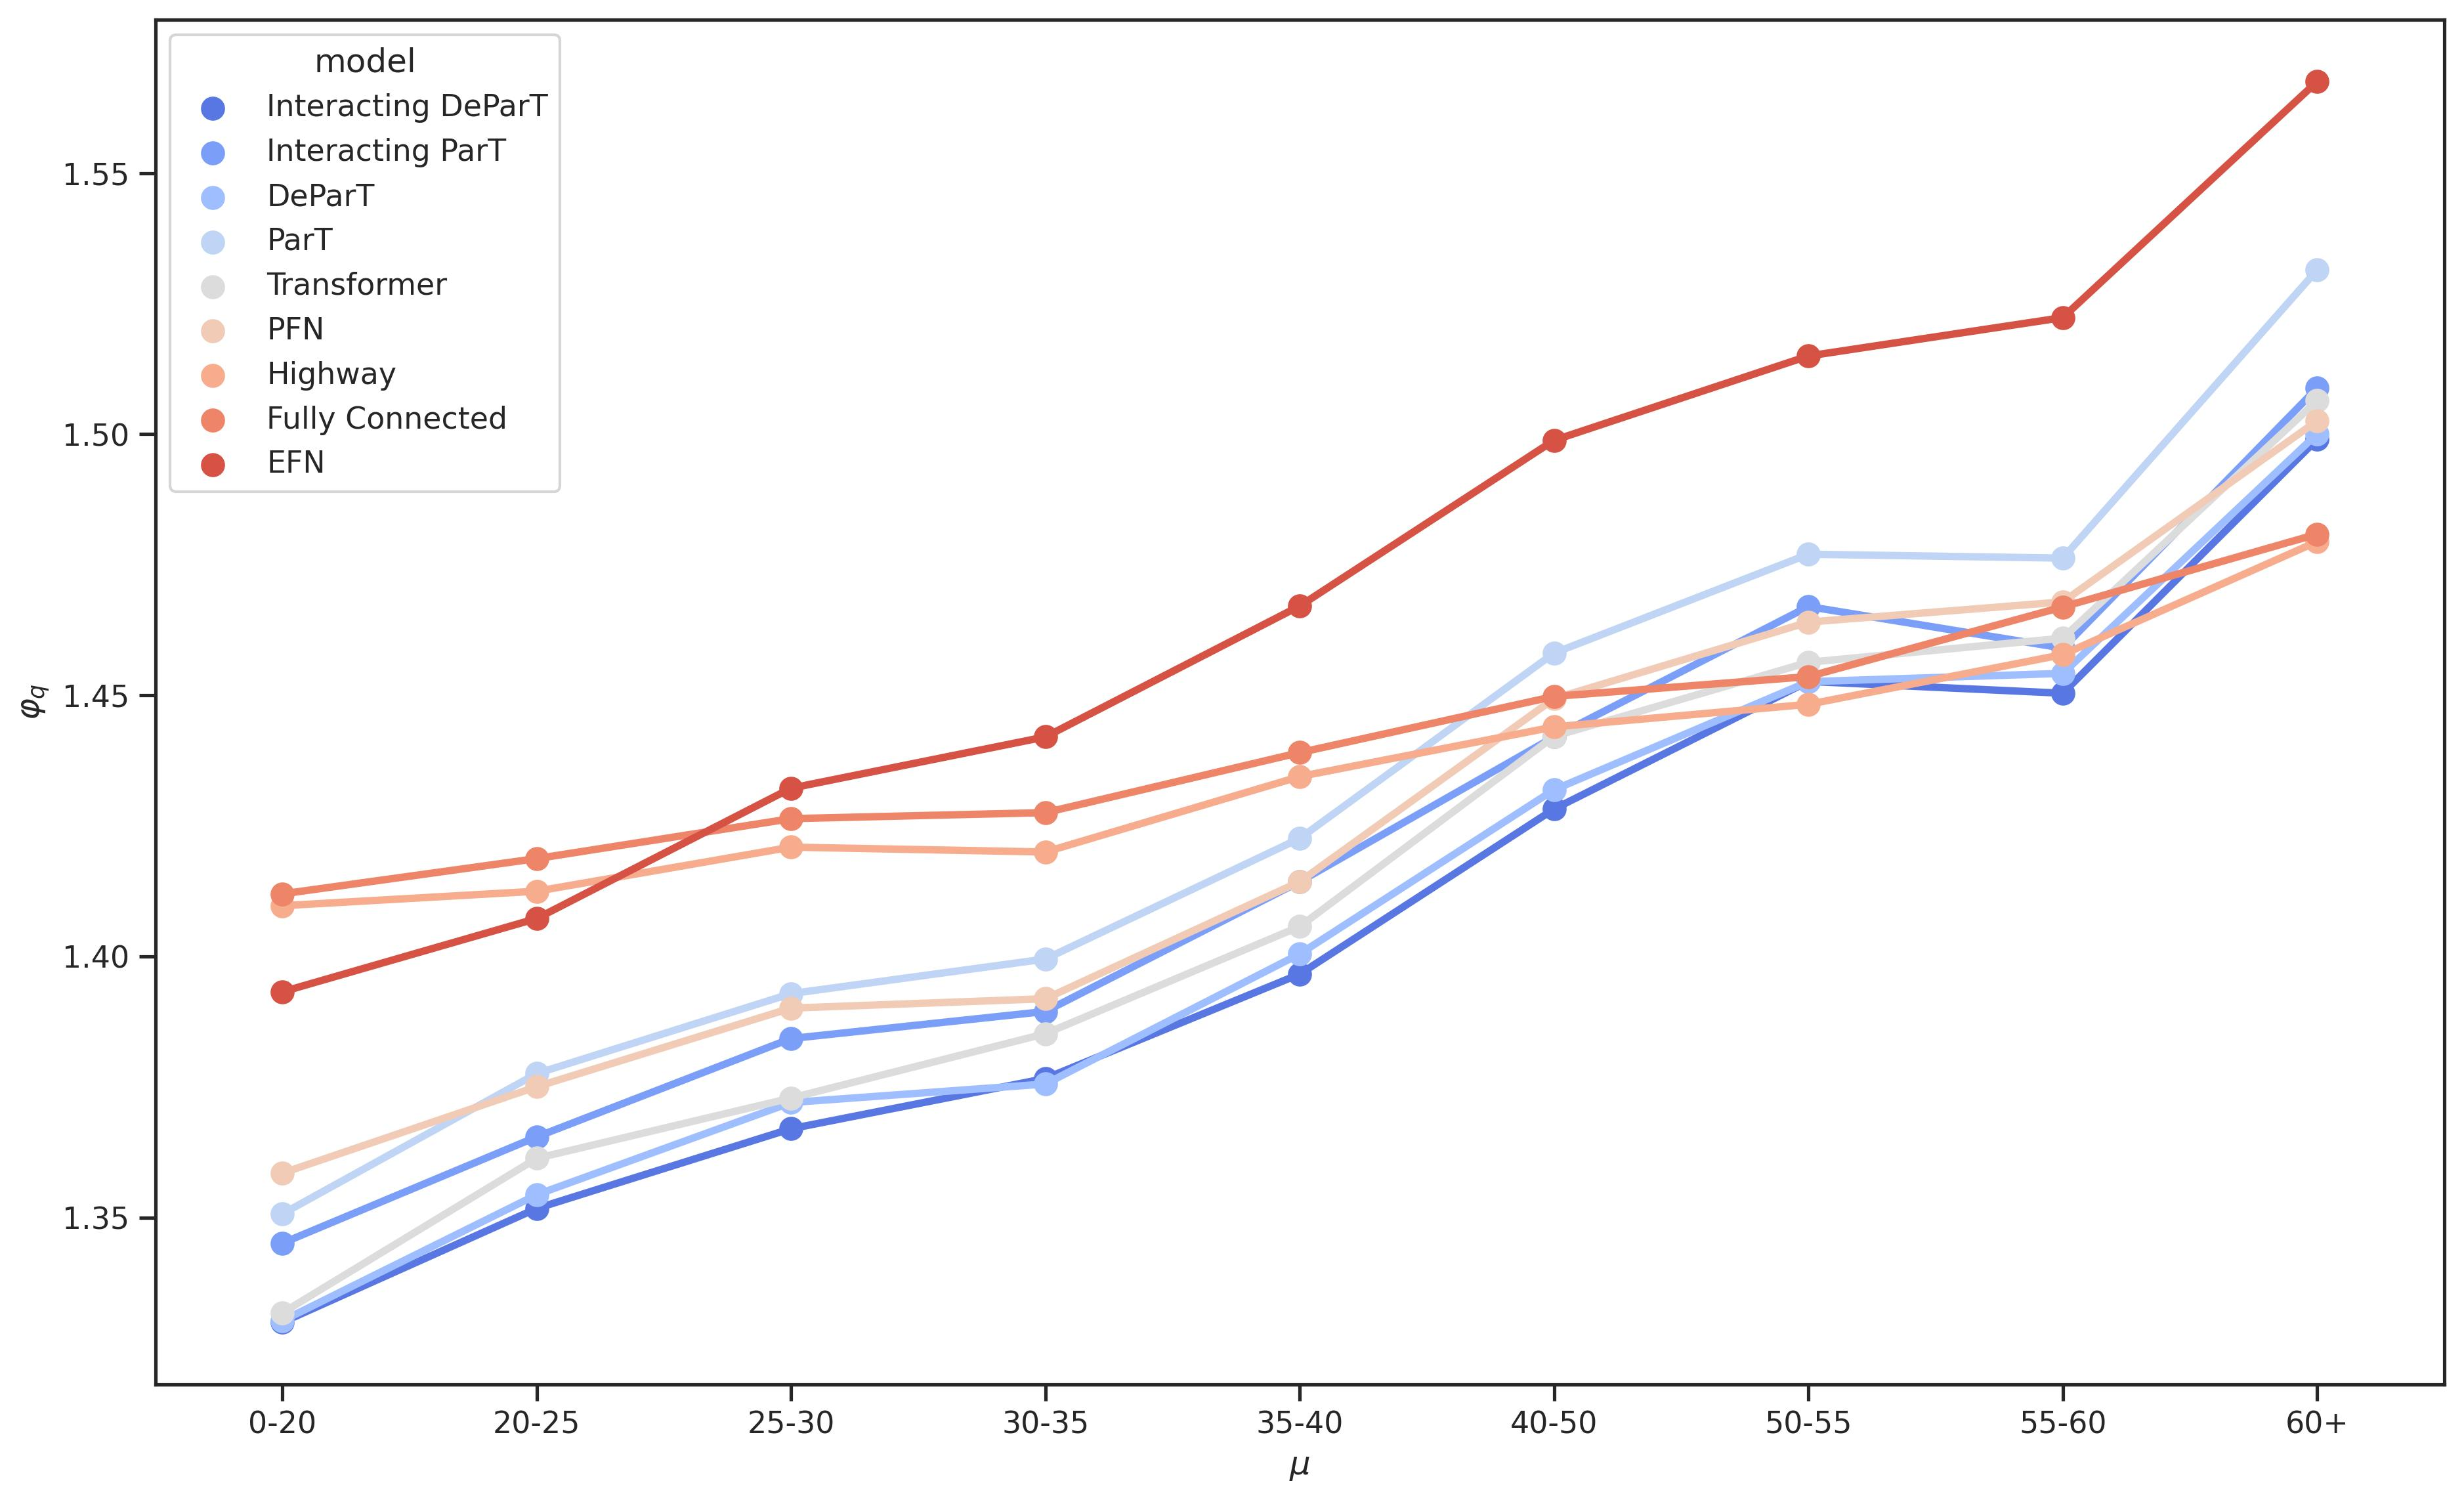
\includegraphics[width=0.95\linewidth]{src/plots/results/mu_dep/quark_rejection.jpg}
    \caption{Quark rejection as a function of pileup.}
    \label{fig:quark_rej_pileup}
\end{figure}

\begin{figure}[htb]
    \centering
    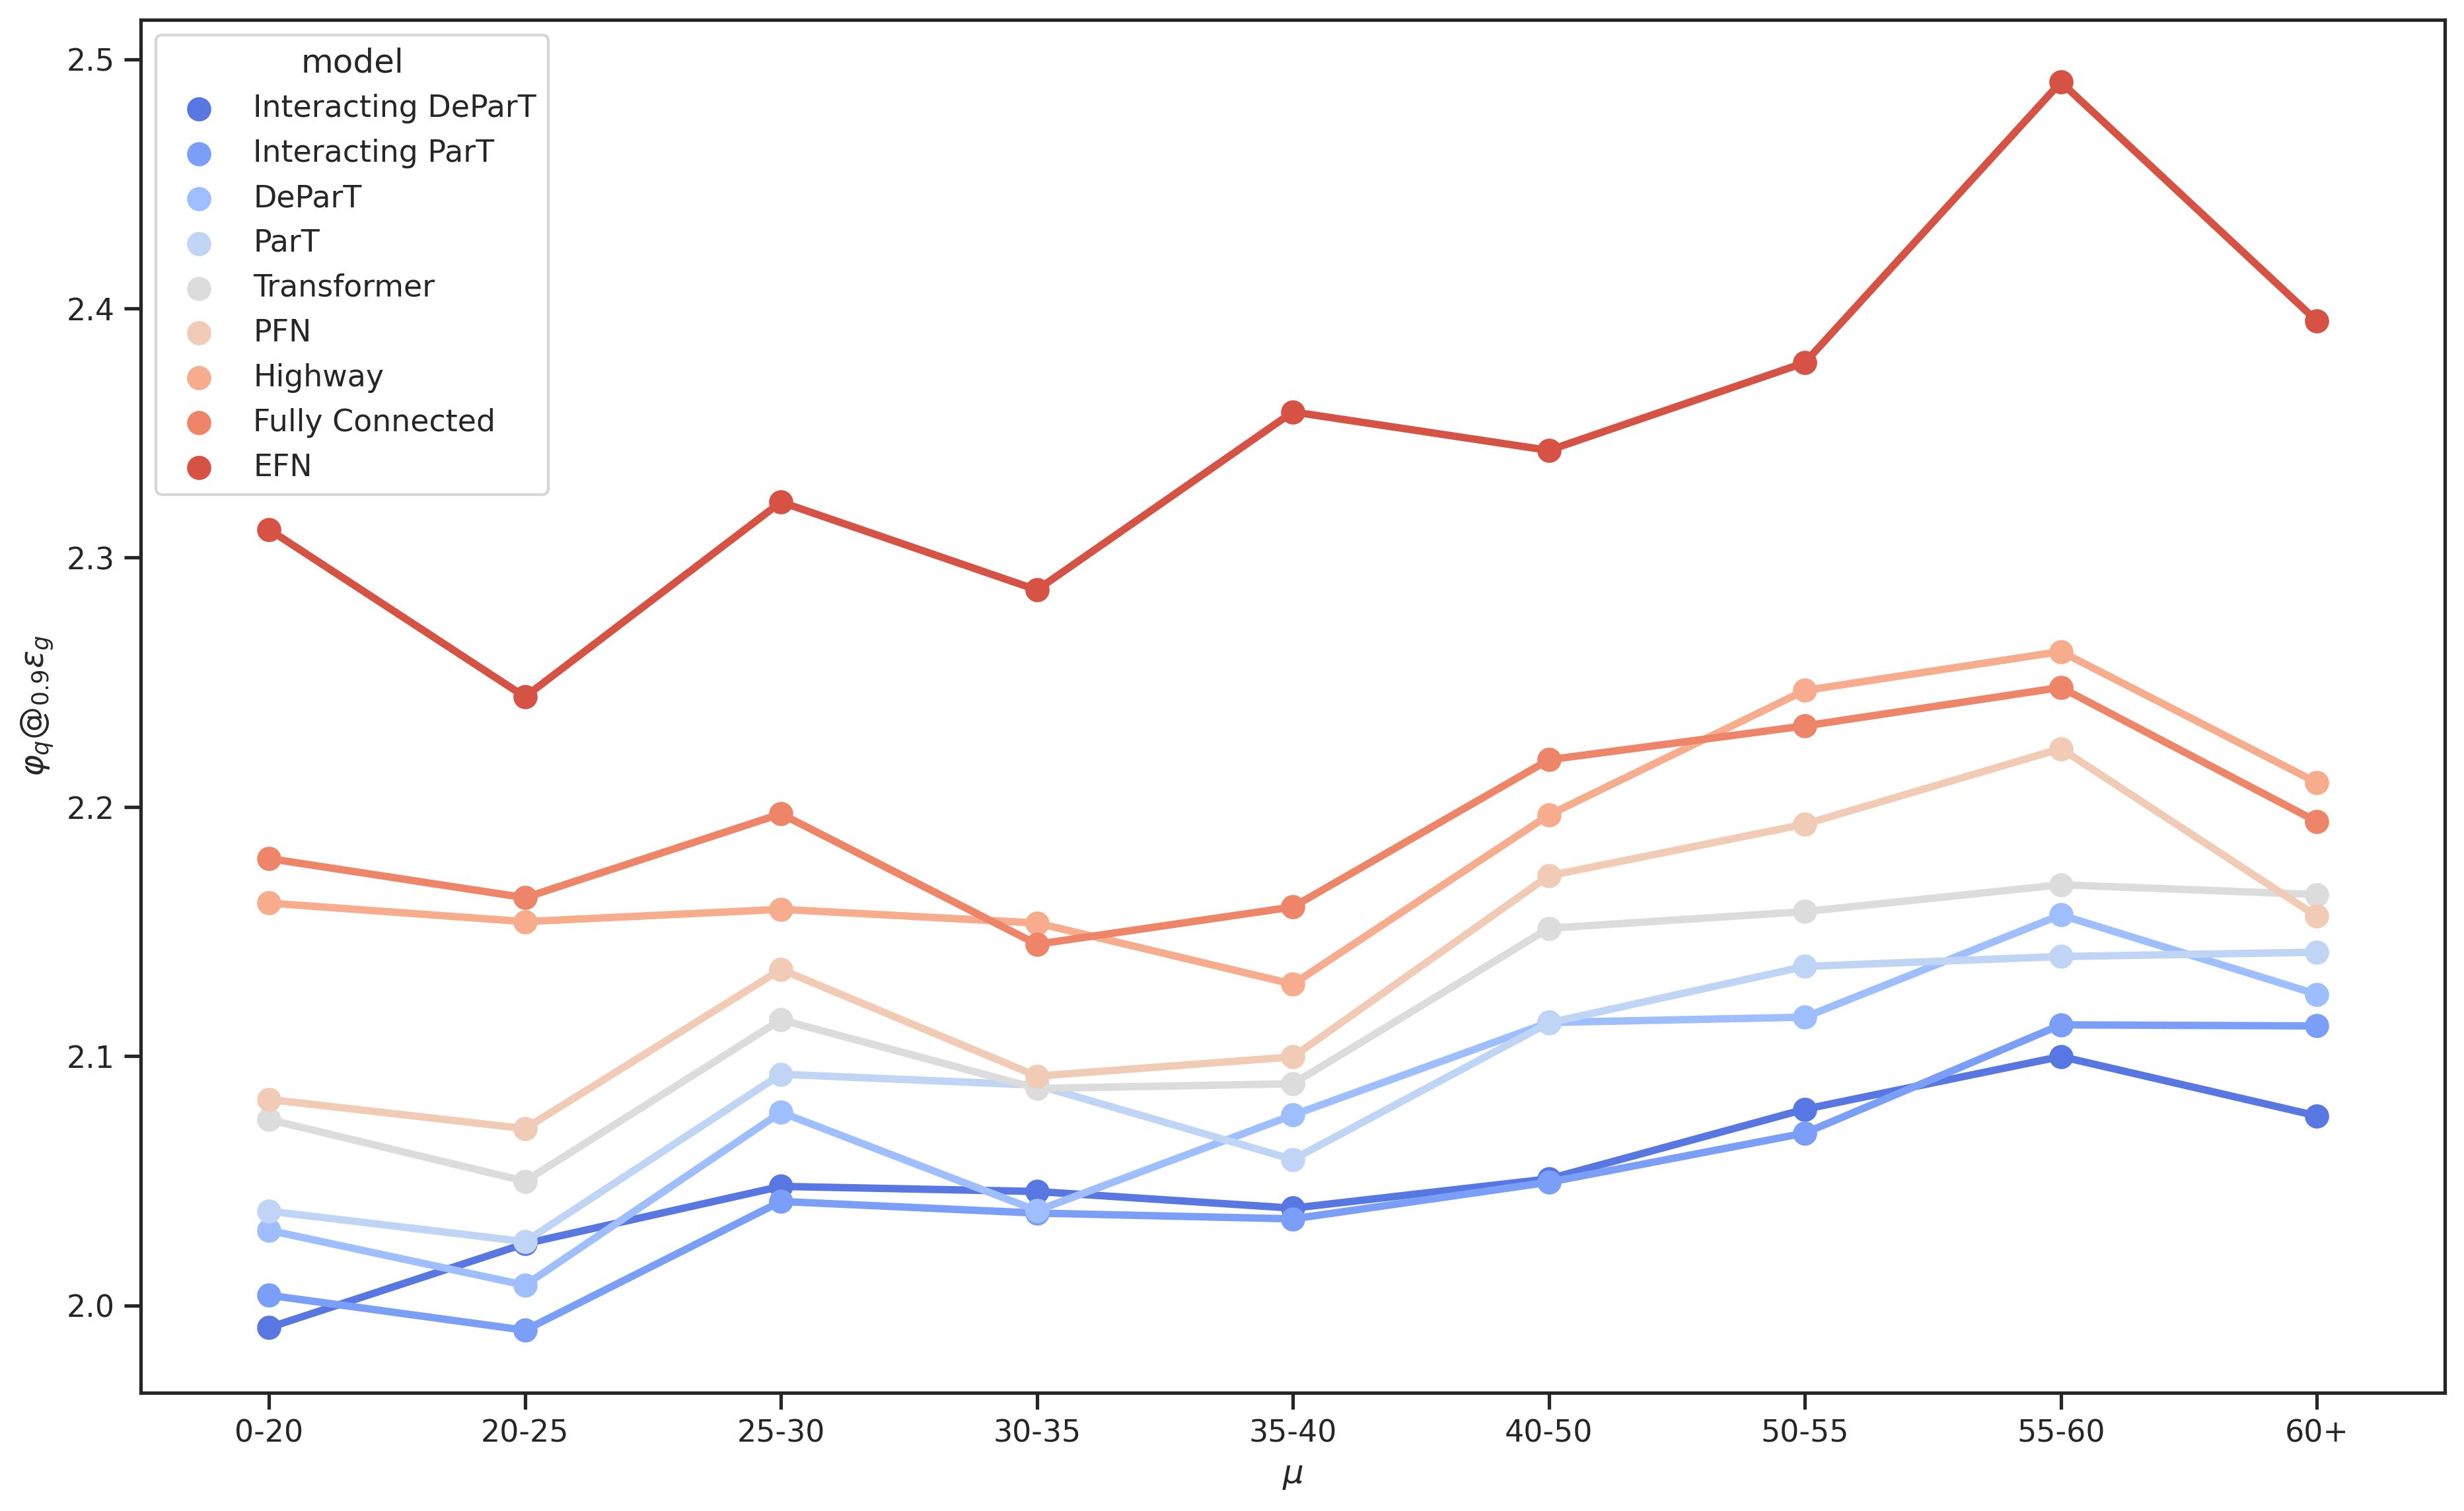
\includegraphics[width=0.95\linewidth]{src/plots/results/mu_dep/quark_rej_at_gluon_eff_0.9.jpg}
    \caption{Quark rejection at gluon efficiency of 0.9 as a function of pileup.}
    \label{fig:quark_rej_at_gluon_eff_0.9_pileup}
\end{figure}

\begin{figure}[htb]
    \centering
    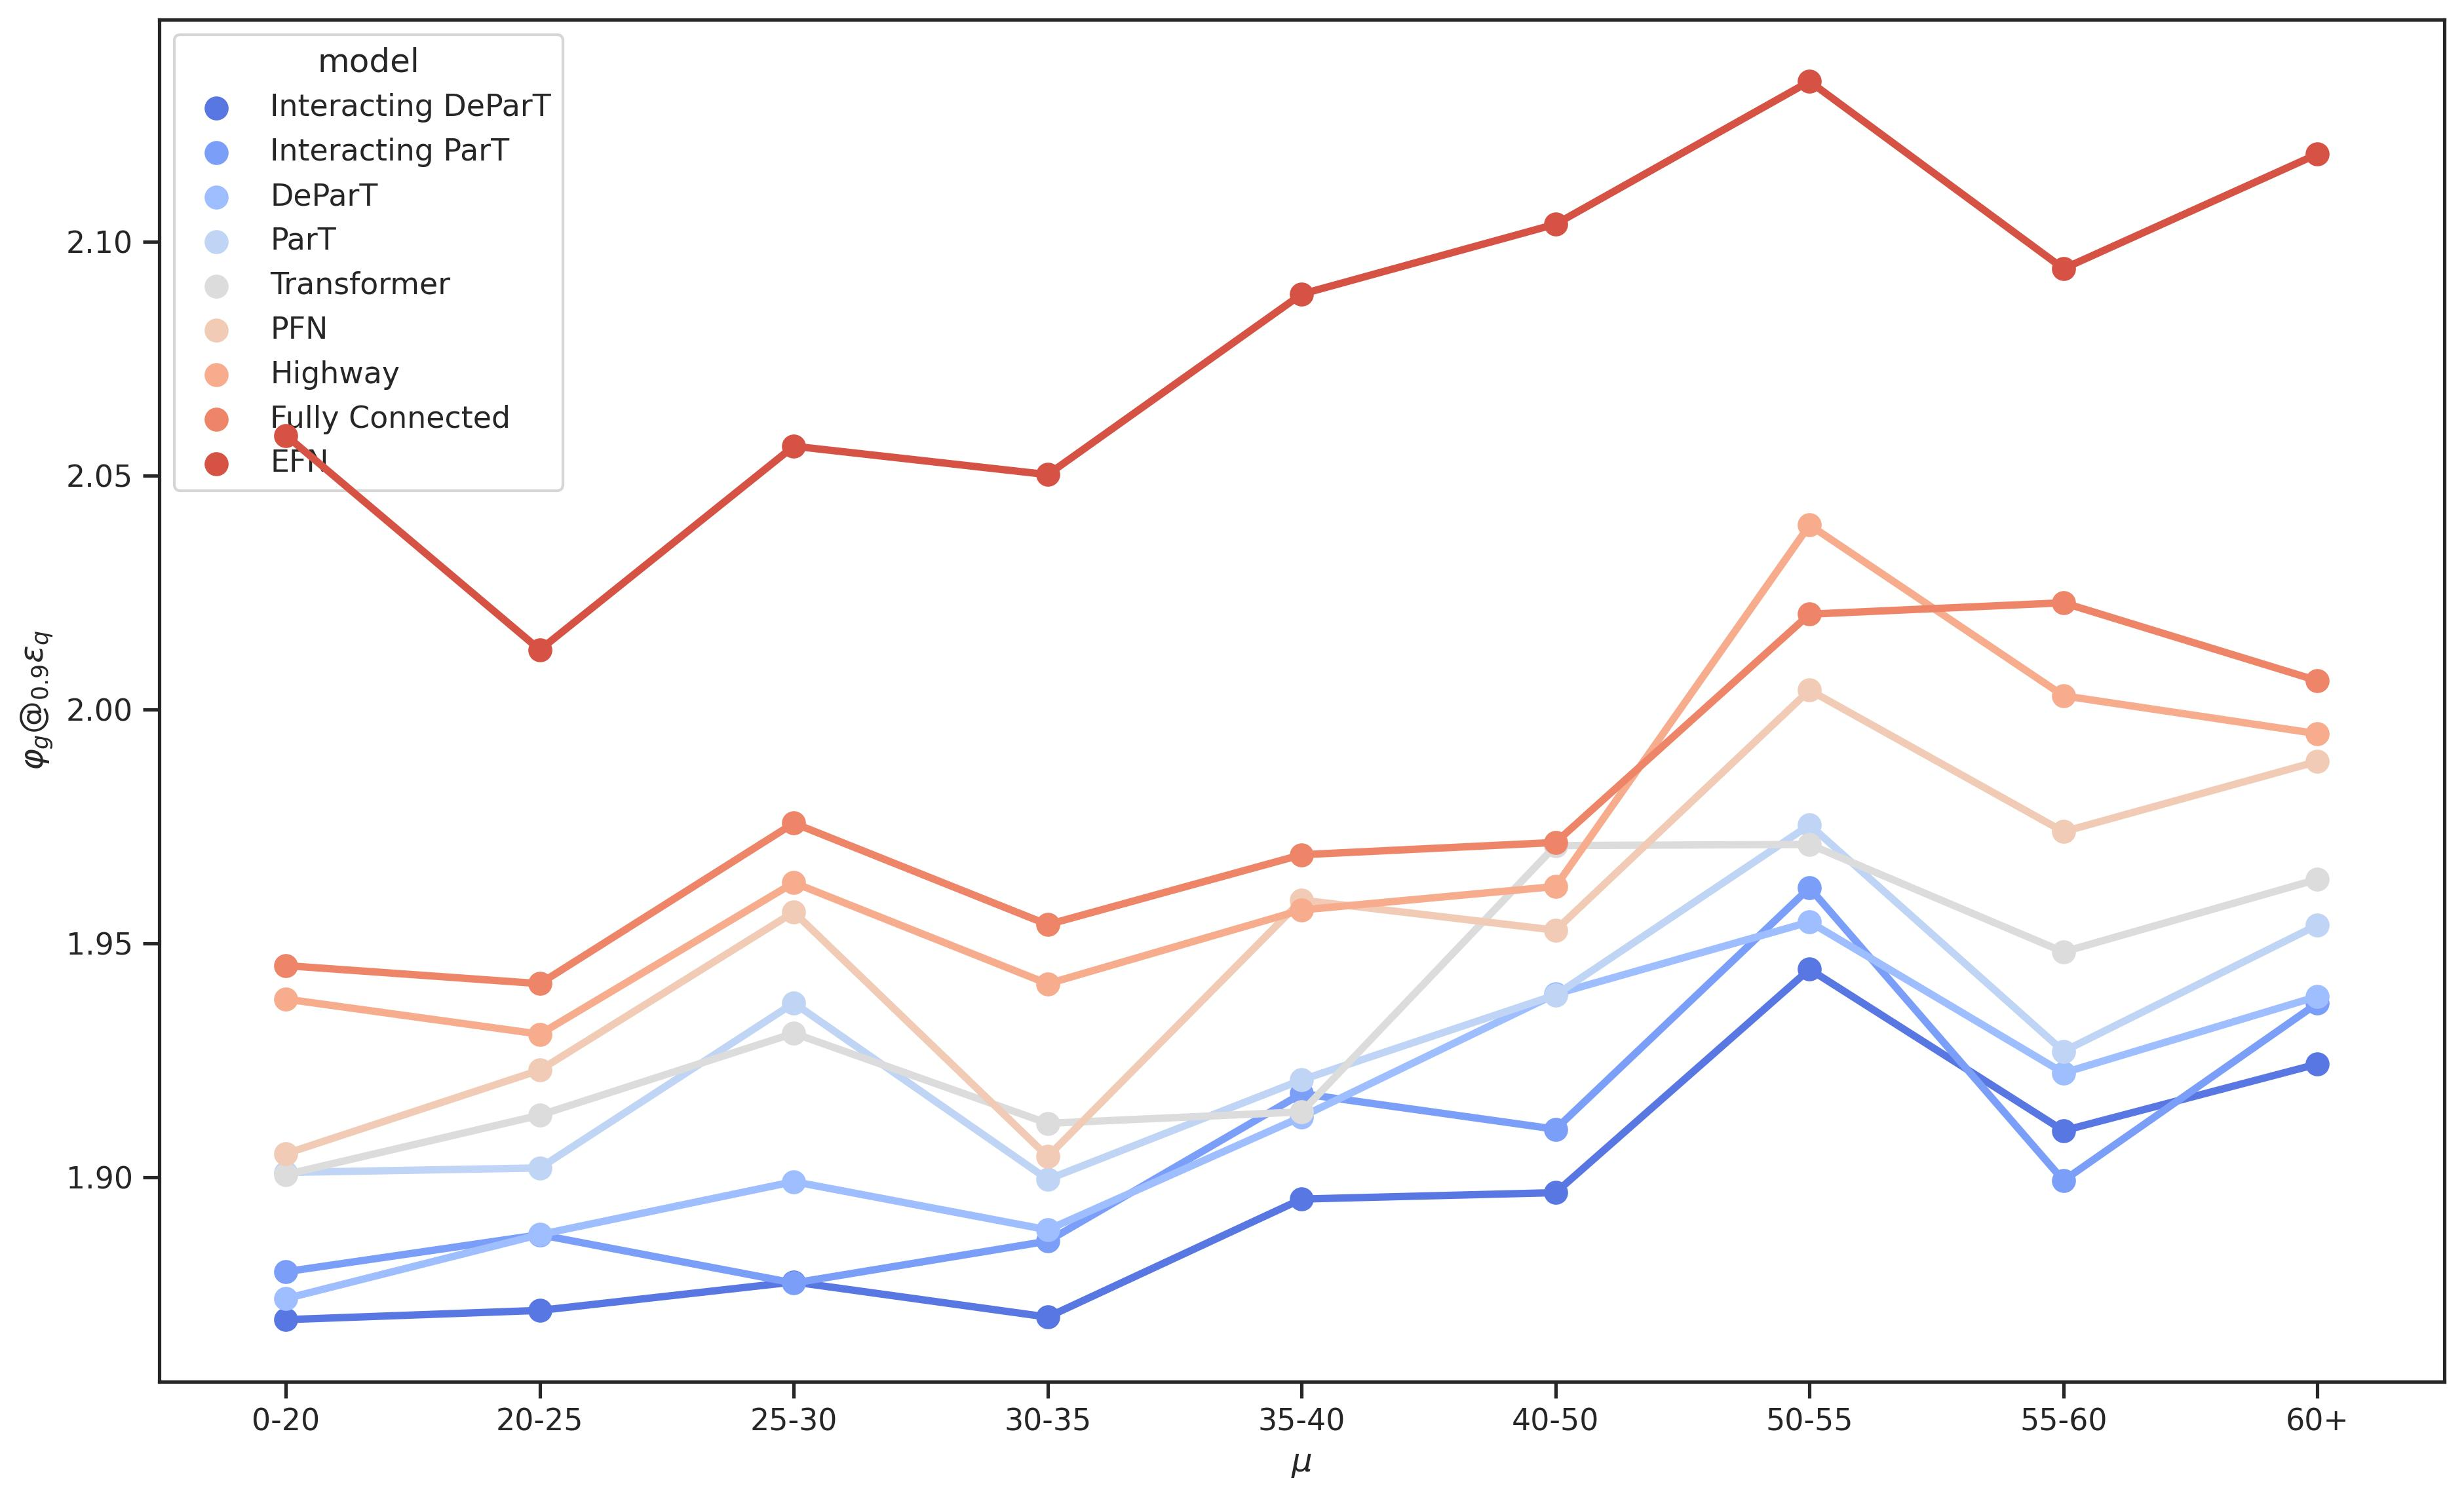
\includegraphics[width=0.95\linewidth]{src/plots/results/mu_dep/gluon_rej_at_quark_eff_0.9.jpg}
    \caption{Gluon rejection at quark efficiency of 0.9 as a function of pileup.}
    \label{fig:gluon_rej_at_quark_eff_0.9_pileup}
\end{figure}

\begin{figure}[htb]
    \centering
    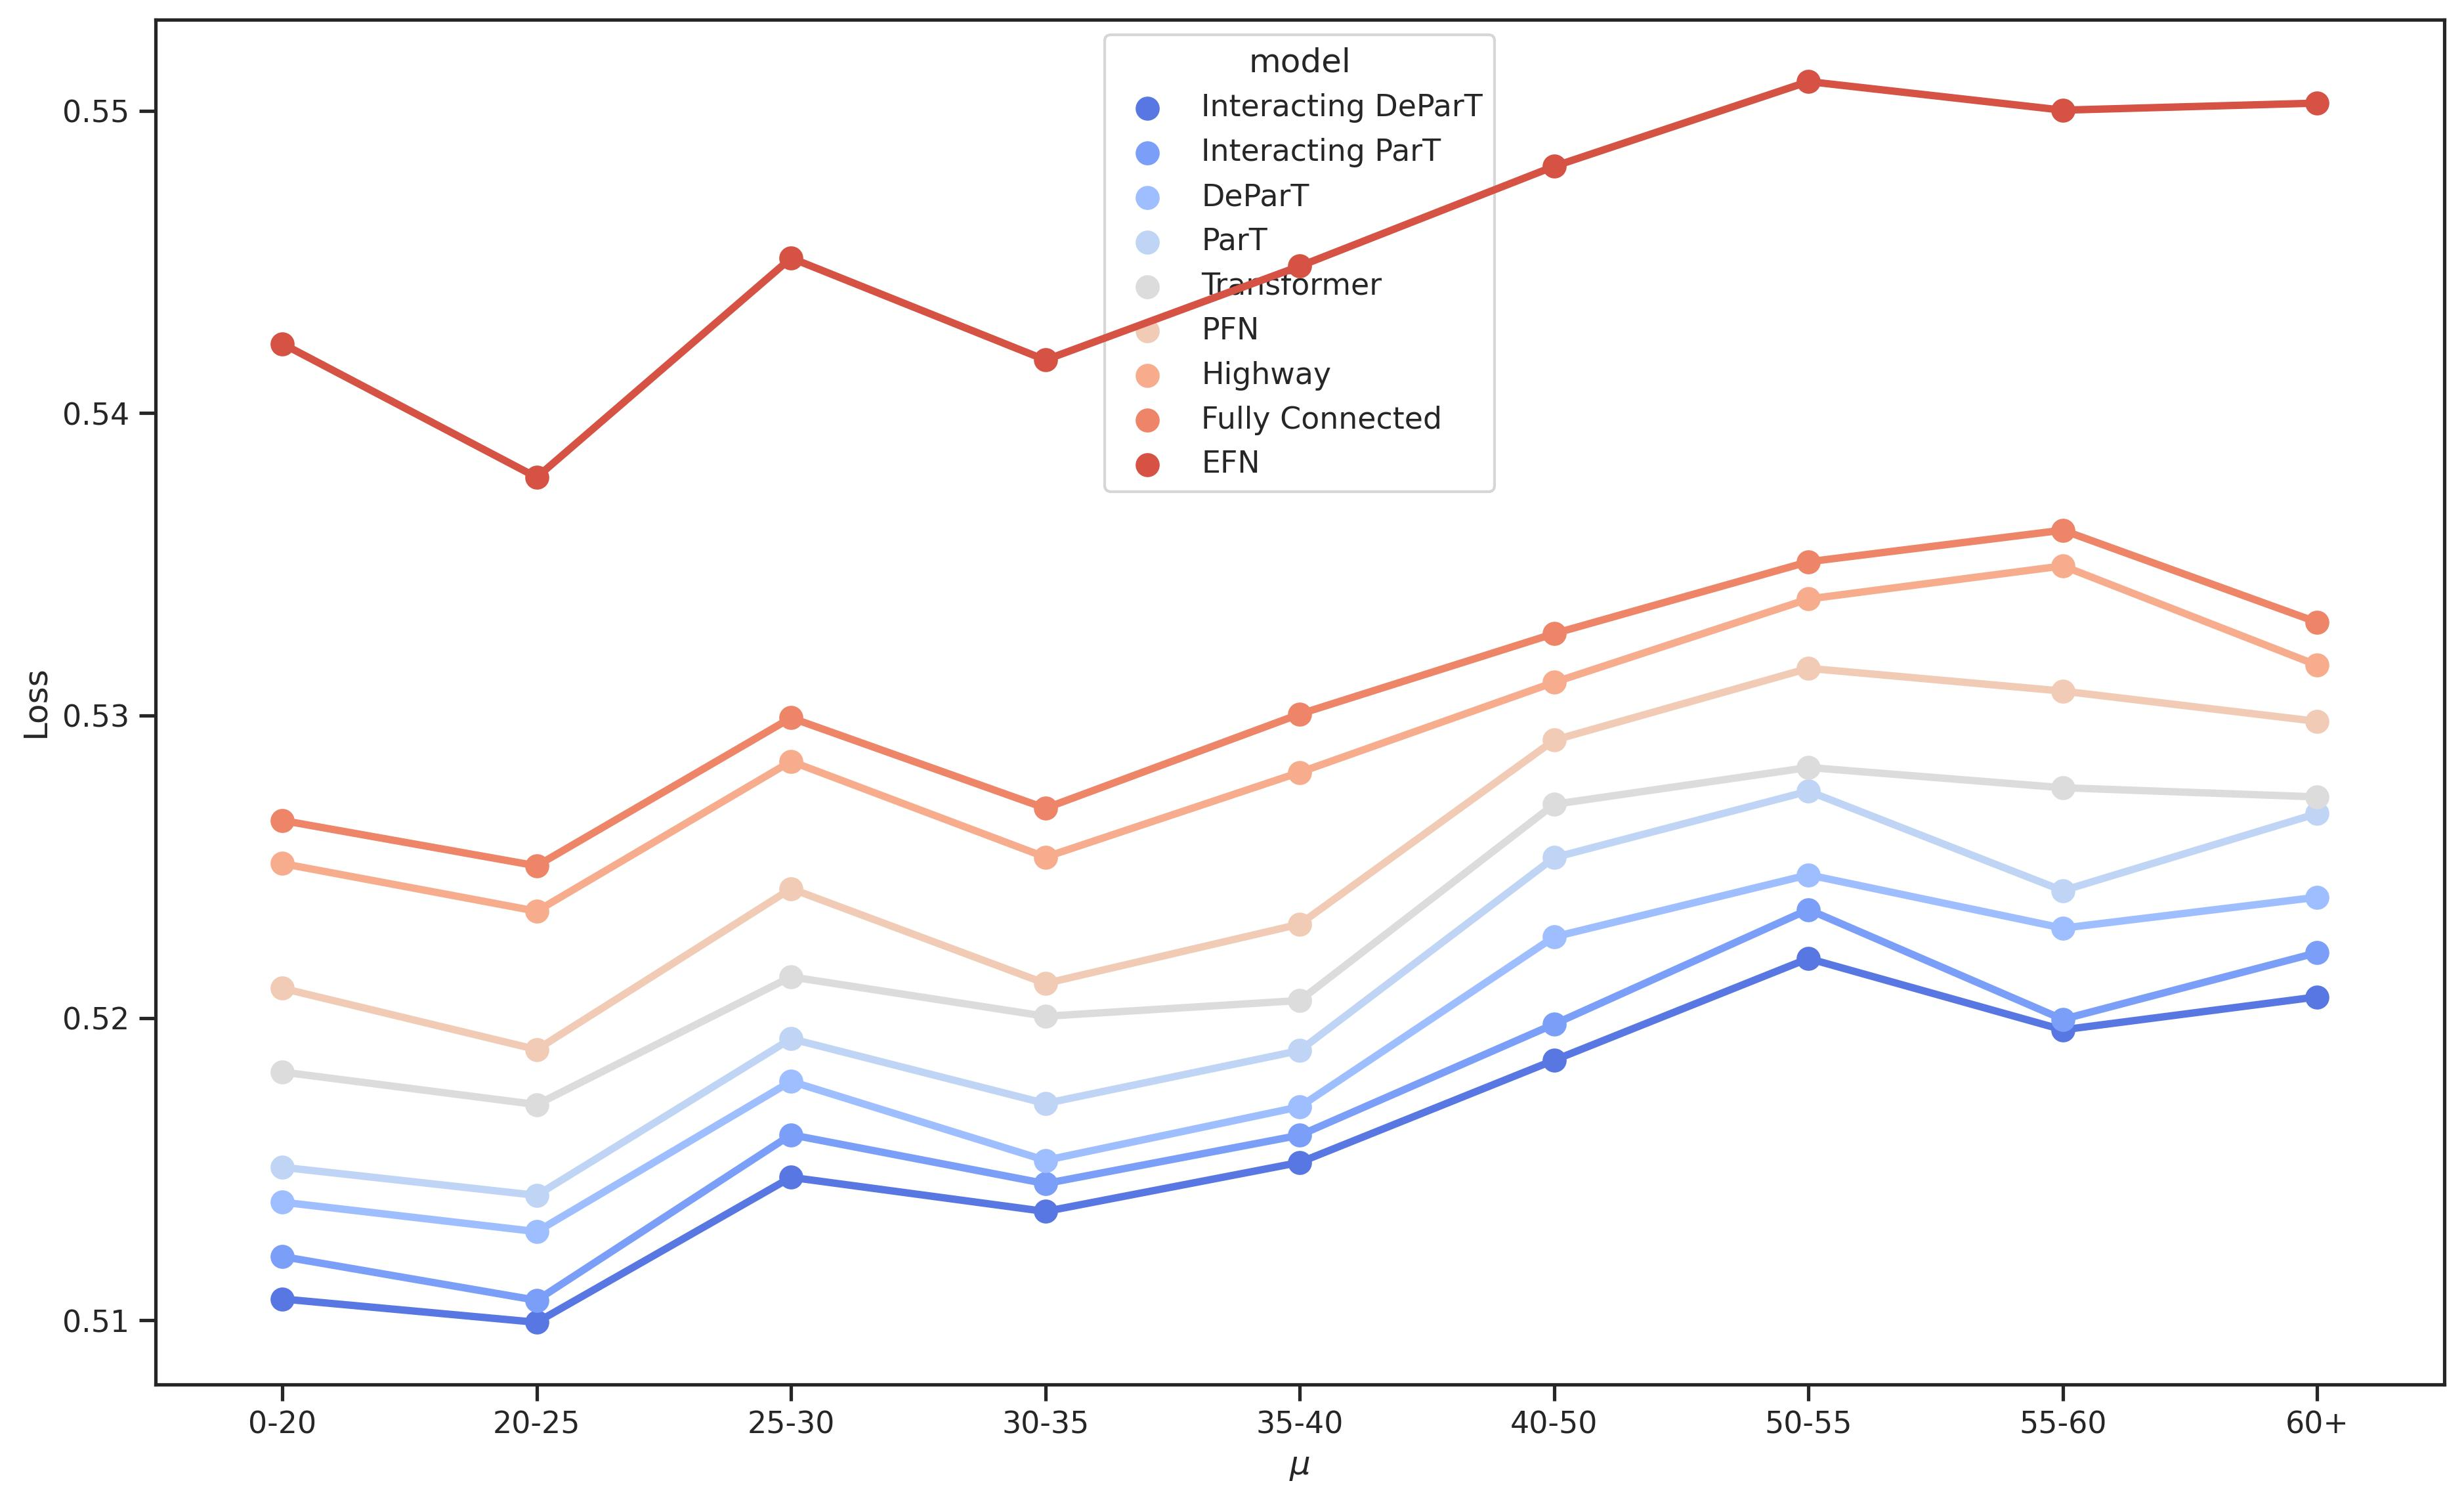
\includegraphics[width=0.95\linewidth]{src/plots/results/mu_dep/loss.jpg}
    \caption{Loss as a function of pileup.}
    \label{fig:loss_pileup}
\end{figure}


